% \documentclass[10pt,aspectratio=43,mathserif,table]{beamer} %这个是4：3的
\documentclass[8pt,aspectratio=169,mathserif,table]{beamer}  %这个是16：9的
%设置为 Beamer 文档类型，设置字体为 10pt，长宽比为16:9，数学字体为 serif 风格

\usepackage{graphicx}
\usepackage{tikz}
\usepackage{animate}
\usepackage{hyperref}

%导入一些用到的宏包
\usepackage{amsmath,bm,amsfonts,amssymb,enumerate,epsfig,bbm,calc,color,ifthen,capt-of,multimedia,hyperref}
\usepackage{xeCJK} %导入中文包
\setCJKmainfont{SimHei} %字体采用黑体
\setCJKsansfont{Microsoft YaHei}
\setCJKmonofont{SimHei}
% 设置英文字体
\setmainfont{Times New Roman}
\setsansfont{Microsoft YaHei}

\usetheme{Berlin} %主题
\usecolortheme{sustech} %主题颜色

% --- 保持标题字号与原来 9pt 一致 ---
\setbeamerfont{frametitle}{size=\fontsize{9pt}{11pt}\bfseries}
\setbeamerfont{framesubtitle}{size=\fontsize{7pt}{9pt}\itshape}
\setbeamerfont{section in head/foot}{size=\fontsize{7pt}{9pt}}
\setbeamerfont{author in head/foot}{size=\fontsize{7pt}{9pt}}
\setbeamerfont{title in head/foot}{size=\fontsize{7pt}{9pt}}
\setbeamerfont{date in head/foot}{size=\fontsize{7pt}{9pt}}
\setbeamerfont{frame reference}{size=\fontsize{5.5pt}{6.6pt}}

% --- 自定义强调色：蓝色加粗 ---
\setbeamercolor{alerted text}{fg=blue}

% --- 为图片和表格开启编号（beamer 默认关闭） ---
\setbeamertemplate{caption}[numbered]

% --- 公式/图/表编号带上节号（如 1.1, 1.2, 2.1）---
\numberwithin{equation}{section}
\numberwithin{figure}{section}
\numberwithin{table}{section}

\usepackage[ruled,linesnumbered]{algorithm2e}
\usepackage{fancybox}
\usepackage{xcolor}
\usepackage{times}
\usepackage{listings}
\usepackage{booktabs}
\usepackage{colortbl}
\usepackage{multirow}
% Chapter 4 使用文本图表替代 tikzpicture/svg，无需额外宏包

\newcommand{\Console}{Console}
\lstset{ %
	backgroundcolor=\color{white},
	basicstyle=\footnotesize\rmfamily,
	columns=fullflexible,
	breaklines=true,
	captionpos=b,
	tabsize=4,
	commentstyle=\color{mygreen},
	escapeinside={\%*}{*)},
	keywordstyle=\color{blue},
	stringstyle=\color{mymauve}\ttfamily,
	numbers=left,
	rulesepcolor=\color{red!20!green!20!blue!20},
	language=c
}

\setsansfont{Microsoft YaHei}
\setmainfont{Times New Roman}

\definecolor{mygreen}{rgb}{0,0.6,0}
\definecolor{mymauve}{rgb}{0.58,0,0.82}
\definecolor{mygray}{gray}{.9}
\definecolor{mypink}{rgb}{.99,.91,.95}
\definecolor{mycyan}{cmyk}{.3,0,0,0}

%题目，作者，学校，日期
\title{光学像差诊断与国产大视场空气物镜设计}
\subtitle{\fontsize{9pt}{14pt}\textbf{Zemax说明及仿真}}
\author{汇报人: 胡子睿}
\institute{\fontsize{10pt}{16pt}Institute of Physics, CAS}
\date{\today}

%学校Logo（如缺少logo图片可注释掉以下两行）
%\pgfdeclareimage[height=0.4cm]{sustech-logo}{Figure/中科院物理所.png}
%\logo{\pgfuseimage{sustech-logo}\hspace*{0.2cm}}

% --- 每节幻灯片自动编号 + 英文副标题 ---
\makeatletter
\newcounter{secframenumber}[section]

\newcommand{\englishtitle}[1]{\def\@englishtitle{#1}}
\let\@englishtitle\@empty

% --- 当前页参考文献文本框：按页设置，在页脚阶段绘制到前景层 ---
\newif\ifshowframerefbox
\showframerefboxfalse
\newcommand{\insertframerefbox}{}
\newcommand{\clearframerefbox}{%
  \global\showframerefboxfalse
  \gdef\insertframerefbox{}%
}
\newcommand{\framerefbox}[1]{%
  \gdef\insertframerefbox{#1}%
  \global\showframerefboxtrue
}
\newcommand{\framecite}[1]{\framerefbox{参考文献：\cite{#1}}}
\BeforeBeginEnvironment{frame}{\clearframerefbox}

% 临时屏蔽当前帧编号（目录页、Thank you 页使用）
\newif\ifnoslidenumber
\newcommand{\nonumberframe}{\global\noslidenumbertrue}

% 编号前缀宽度（确保中英标题对齐）
\newlength{\numberwidth}
\setlength{\numberwidth}{2.5em}

% 页脚与参考文献框对齐参数
\newlength{\footlineheight}
\setlength{\footlineheight}{3.625ex}

\setbeamertemplate{frametitle}
{%
  \ifbeamercolorempty[bg]{frametitle}{}{\nointerlineskip}%
  \begin{beamercolorbox}[sep=0.18cm,left,wd=\paperwidth]{frametitle}
    \usebeamerfont{frametitle}%
    \ifnoslidenumber
      \ifnum\value{section}>0\relax
        \makebox[\numberwidth][r]{}\hspace{0.4em}\insertframetitle\par
      \else
        \insertframetitle\par
      \fi
      \global\noslidenumberfalse
    \else
      \stepcounter{secframenumber}%
      \ifnum\value{section}>0%
        \makebox[\numberwidth][r]{\thesection.\arabic{secframenumber}}\hspace{0.4em}\insertframetitle\par%
      \else%
        \insertframetitle\par%
      \fi%
    \fi
    \ifx\@englishtitle\@empty\else%
      \vskip1pt\relax
      {\usebeamerfont{framesubtitle}\itshape\makebox[\numberwidth][r]{}\hspace{0.4em}\@englishtitle\par}%
      \global\let\@englishtitle\@empty%
    \fi%
  \end{beamercolorbox}%
}
\makeatother

% --- 导航栏：仅显示可点击的 section 标题 ---
\setbeamertemplate{headline}
{%
  \begin{beamercolorbox}[colsep=1.5pt]{upper separation line head}
  \end{beamercolorbox}
  \begin{beamercolorbox}{section in head/foot}
    \vskip2pt\insertsectionnavigationhorizontal{\paperwidth}{}{\hskip0pt plus1filll}\vskip2pt
  \end{beamercolorbox}%
  \begin{beamercolorbox}[colsep=1.5pt]{lower separation line head}
  \end{beamercolorbox}
}

% --- 页脚：作者（左） | 标题 — 26/40（右）---
\setbeamertemplate{footline}
{%
  \leavevmode%
  \hbox{%
    \begin{beamercolorbox}[wd=.5\paperwidth,ht=2.5ex,dp=1.125ex,leftskip=.3cm,rightskip=.3cm]{author in head/foot}%
      \usebeamerfont{author in head/foot}\insertshortauthor
    \end{beamercolorbox}%
    \begin{beamercolorbox}[wd=.5\paperwidth,ht=2.5ex,dp=1.125ex,leftskip=.3cm,rightskip=.3cm plus1fil]{title in head/foot}%
      \usebeamerfont{title in head/foot}\insertshorttitle\nobreak\hfill\nobreak%
      \usebeamerfont{date in head/foot}\insertshortdate{}\hspace*{1em}%
      \insertframenumber{} / \inserttotalframenumber\hspace*{1ex}%
    \end{beamercolorbox}%
  }%
  \ifshowframerefbox
    \begin{tikzpicture}[remember picture,overlay]
      \node[
        anchor=south west,
        xshift=.08cm,
        yshift=\footlineheight,
        rounded corners=2pt,
        draw=black!25,
        fill=white,
        text width=.62\paperwidth,
        inner xsep=5pt,
        inner ysep=3pt
      ] at (current page.south west) {%
        \usebeamerfont{frame reference}\color{black}\insertframerefbox
      };
    \end{tikzpicture}%
  \fi
  \vskip0pt%
}
\AtBeginSection[]
{
	\nonumberframe
	\begin{frame}
	\frametitle{\textbf{目录}}
	\label{toc:\thesection}
	\tableofcontents[currentsection]
	\end{frame}
}
% 注意：以下行已删除 —— \beamerdefaultoverlayspecification{<+->}
% 所有列表项将在单页内同时显示，不再逐条分页

% -----------------------------------------------------------------------------
\begin{document}
% -----------------------------------------------------------------------------

\begin{frame}
\label{titlepage}
\titlepage
\end{frame}

% -----------------------------------------------------------------------------

\section{像差理论与诊断基础}
\label{chap:1}

\subsection{统一框架：先定义理想，再分析偏离}
\label{sec:1.1}

\englishtitle{One Story for Aberration Analysis}
\begin{frame}{本报告的主线}
\label{1.1}
    \begin{columns}[T]
        \begin{column}{.52\textwidth}
            \textbf{目标：}把“像差是什么”收束成一条可以在 Zemax 中验证和优化的链路：

            \begin{center}
                \fbox{\textbf{理想成像}}\quad
                $\rightarrow$\quad
                \fbox{\textbf{OPD/波前}}\quad
                $\rightarrow$\quad
                \fbox{\textbf{Ray Fan/Zernike}}\quad
                $\rightarrow$\quad
                \fbox{\textbf{PSF/MTF}}
            \end{center}

            \bigbreak
            \begin{itemize}
                \item \alert{理想成像}给出参考：物点应成像为像点。
                \item \alert{OPD}描述实际波前偏离参考球面的程度。
                \item \alert{Ray Fan}从光线落点诊断像差形状。
                \item \alert{Zernike}把波前拆成可量化的正交模式。
                \item \alert{PSF/MTF}回答最终图像是否足够清晰。
            \end{itemize}
        \end{column}
        \hfill
        \begin{column}{.48\textwidth}
            \begin{block}{重构后的删减原则}
                \begin{enumerate}
                    \item 像差定义只讲一次：用 OPD 统一几何与波动描述。
                    \item 一阶量和三阶像差合并讲：前者定系统，后者看残差。
                    \item 色差不单独重复成一章：并入材料色散和 Ray Fan 诊断。
                    \item Zemax 不只列菜单：每个工具都回到同一条像质主线。
                \end{enumerate}
            \end{block}

            \begin{alertblock}{一句话主题}
                从波前误差出发，用 Ray Fan 与 Zernike 找到像差来源，再用 Zemax 把设计推向可制造的像质目标。
            \end{alertblock}
        \end{column}
    \end{columns}
\end{frame}

\englishtitle{First-Order Layout, Third-Order Aberration and Zernike}
\begin{frame}{一阶、三阶与 Zernike 的关系}
\label{1.2}
    \begin{columns}[T]
        \begin{column}{.48\textwidth}
            \begin{alertblock}{先澄清一个容易混淆的点}
                这里的\alert{一阶}不是“一阶色散”，而是近轴高斯光学中的系统规格；\alert{三阶}也不是“三阶色散”，而是去除理想成像后最先出现的 Seidel 像差项。
            \end{alertblock}

            \textbf{一阶设计量回答：系统应该把像成在哪里？}
            \begin{itemize}
                \item 有效焦距 $f'$、放大率 $\beta$、像高 $y'$
                \item 孔径、$F/\#$、NA、视场角 $\omega$
                \item 工作距离、后焦距、系统总长
            \end{itemize}

            \begin{equation}
                \beta = \frac{y'}{y}, \qquad
                J = nyu = n'y'u'
                \label{eq:first_order_main}
            \end{equation}
        \end{column}
        \hfill
        \begin{column}{.52\textwidth}
            \textbf{三阶像差回答：系统偏离理想成像的最低阶形状是什么？}
            \begin{itemize}
                \item 球差：孔径三次项，轴上也存在
                \item 彗差：孔径二次项，随视场一次增长
                \item 像散/场曲：孔径一次项，随视场二次增长
                \item 畸变：主光线像高偏移，主要改变几何相似性
            \end{itemize}

            \begin{block}{Zernike 的位置}
                Zernike 不是另一套重复分类，而是把\alert{波像差 $W(\rho,\theta)$}投影到单位圆上的正交基。它适合把 Zemax 的 OPD 图、干涉测量结果和优化目标连接起来。
            \end{block}
        \end{column}
    \end{columns}
\end{frame}

\subsection{OPD、PSF 与 Ray Fan}
\label{sec:1.2}

\englishtitle{Optical Path Difference and Wave Aberration}
\begin{frame}{OPD：统一描述像差的物理量}
\label{1.3}
    \begin{columns}[T]
        \begin{column}{.52\textwidth}
            \textbf{光程(Optical Path Length)：}
            \begin{equation}
                OPL = \int n(s)\,ds
                \label{eq:opl_main}
            \end{equation}

            \textbf{光程差(OPD)或波像差：}
            \begin{equation}
                OPD = OPL_{\text{actual}} - OPL_{\text{reference}}
                \equiv W(\rho,\theta)
                \label{eq:opd_main}
            \end{equation}

            \textbf{相位误差：}
            \begin{equation}
                \Delta\phi(\rho,\theta)
                = \frac{2\pi}{\lambda}W(\rho,\theta)
                \label{eq:phase_main}
            \end{equation}
        \end{column}
        \hfill
        \begin{column}{.48\textwidth}
            \begin{block}{理想成像的波前条件}
                从同一物点出发并到达同一理想像点的所有光线，应具有相同光程；等价地，实际波前应与以理想像点为球心的参考球面重合。
            \end{block}

            \textbf{广义光瞳函数：}
            \begin{equation}
                P(\rho,\theta)=A(\rho,\theta)
                \exp\!\left[i\frac{2\pi}{\lambda}W(\rho,\theta)\right]
                \label{eq:pupil_main}
            \end{equation}

            \alert{核心判断：}如果 $W=0$，系统只受衍射限制；如果 $W\neq0$，相位误差会改变焦点附近的能量分布。
        \end{column}
    \end{columns}
\end{frame}

\englishtitle{PSF, OTF and Image Formation}
\begin{frame}{PSF 与成像模型：这页才对应 PSF 图片}
\label{1.4}
    \begin{columns}[T]
        \begin{column}{.42\textwidth}
            \begin{figure}
                \centering
                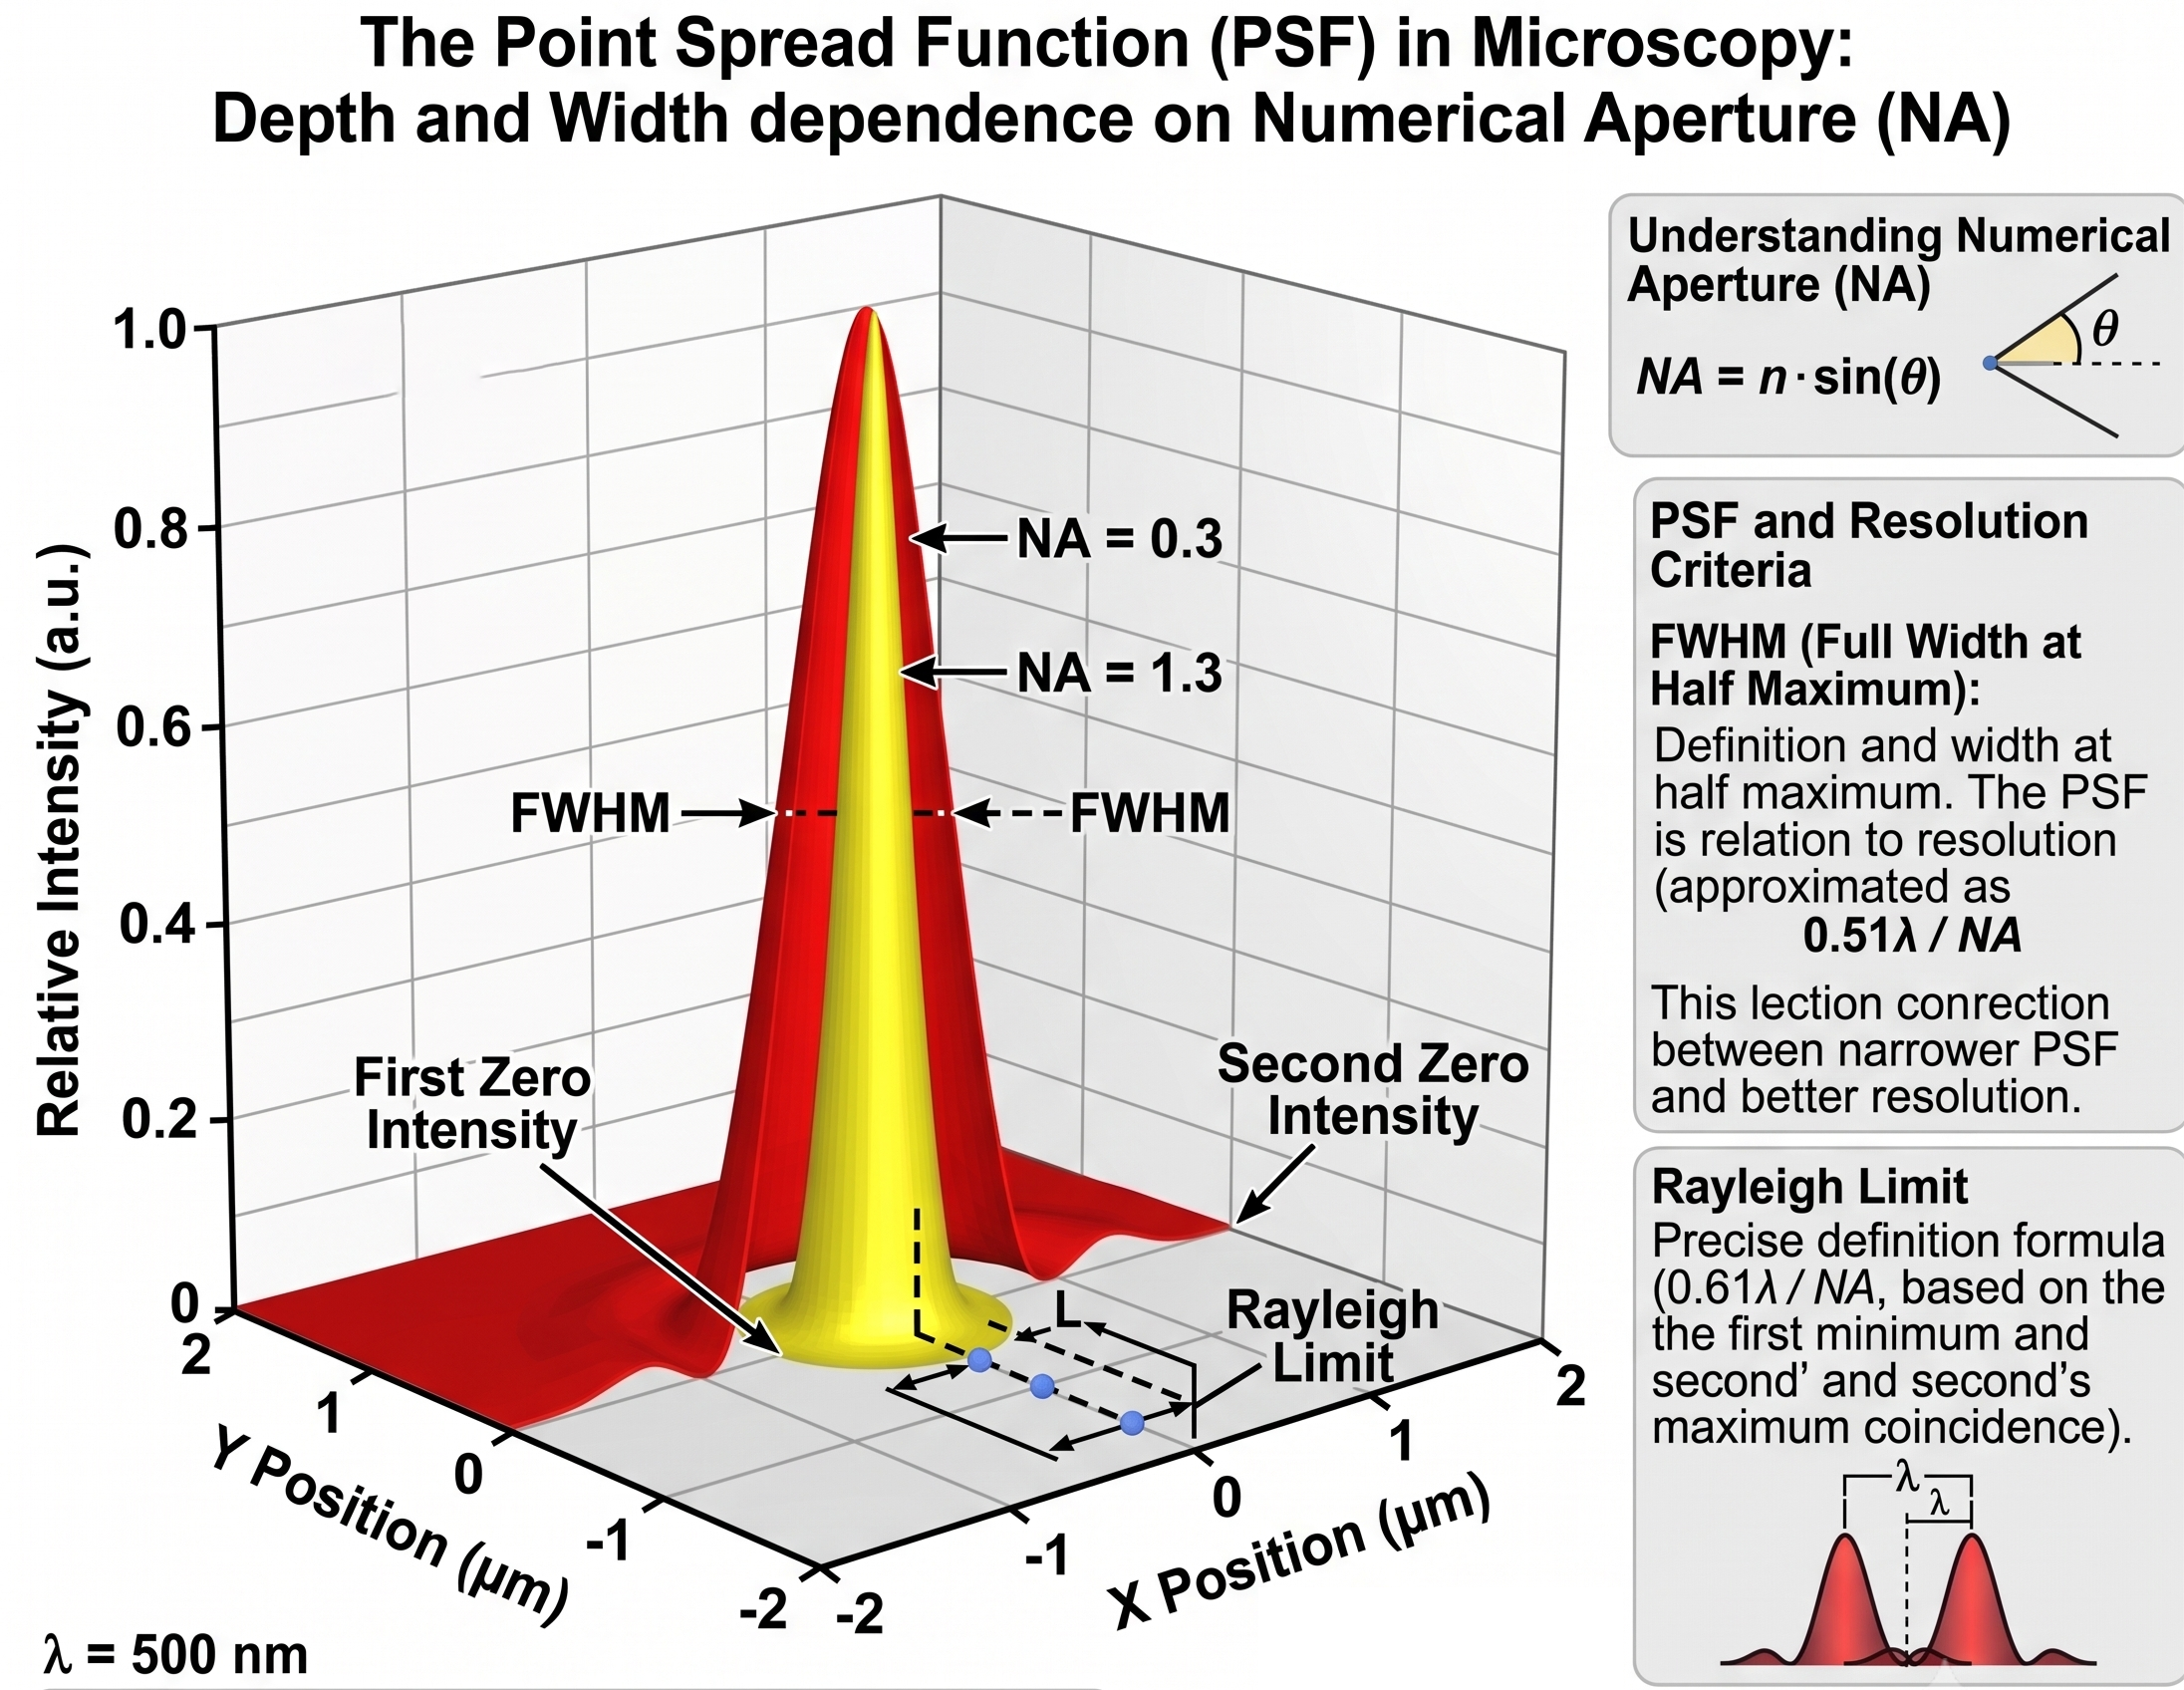
\includegraphics[width=.94\textwidth,height=.42\textheight,keepaspectratio]{Figure/PSF_01.png}
                \caption{PSF、FWHM 与 NA 的关系}
                \label{fig:psf_na_main}
            \end{figure}
        \end{column}
        \hfill
        \begin{column}{.58\textwidth}
            \begin{figure}
                \centering
                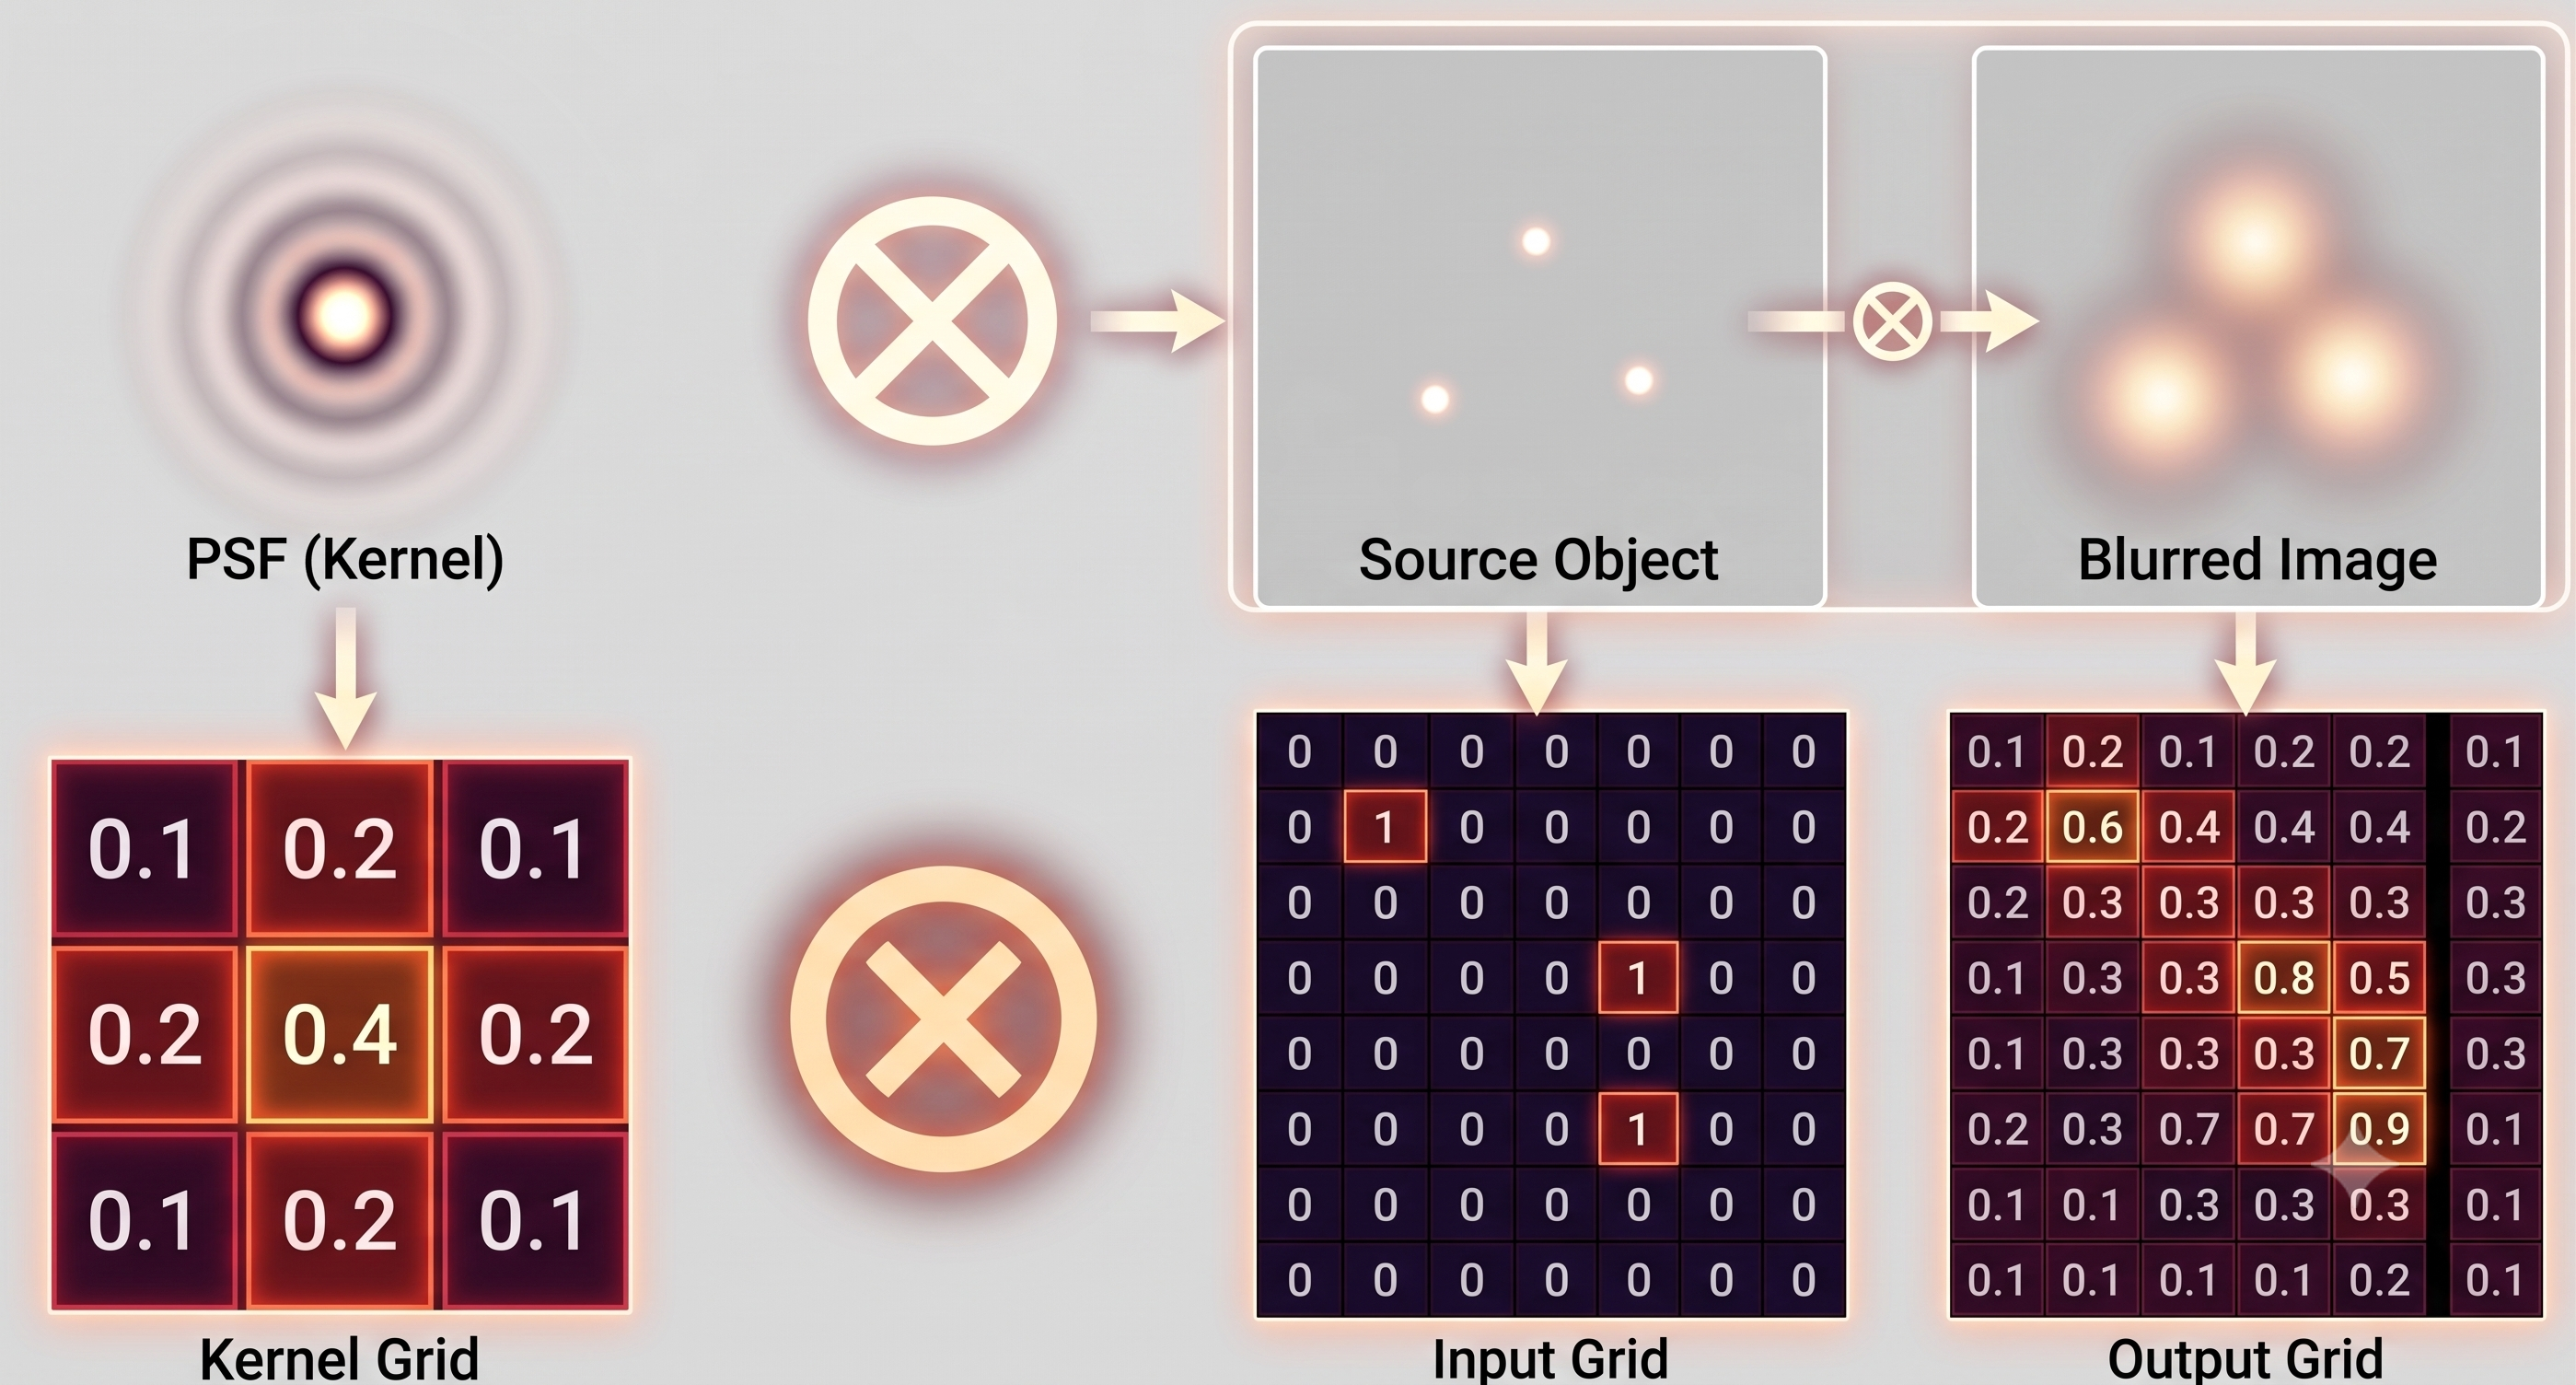
\includegraphics[width=.96\textwidth,height=.30\textheight,keepaspectratio]{Figure/PSF_02.png}
                \caption{物体与 PSF 卷积形成退化图像}
                \label{fig:psf_conv_main}
            \end{figure}

            \vspace{-4pt}
            \begin{equation}
                PSF=\left|\mathcal{F}\{P(\rho,\theta)\}\right|^2,
                \qquad i=o\otimes PSF
                \label{eq:psf_conv_main}
            \end{equation}

            \begin{equation}
                r_{\text{Airy}} = \frac{0.61\lambda}{NA}, \qquad
                OTF=\mathcal{F}\{PSF\}
                \label{eq:airy_otf_main}
            \end{equation}
        \end{column}
    \end{columns}
\end{frame}

\englishtitle{Ray Fan Plot and Its Geometric Meaning}
\begin{frame}{横向像差图：从入瞳采样到像面落点}
\label{1.5}
    \begin{columns}[T]
        \begin{column}{.50\textwidth}
            \begin{figure}
                \centering
                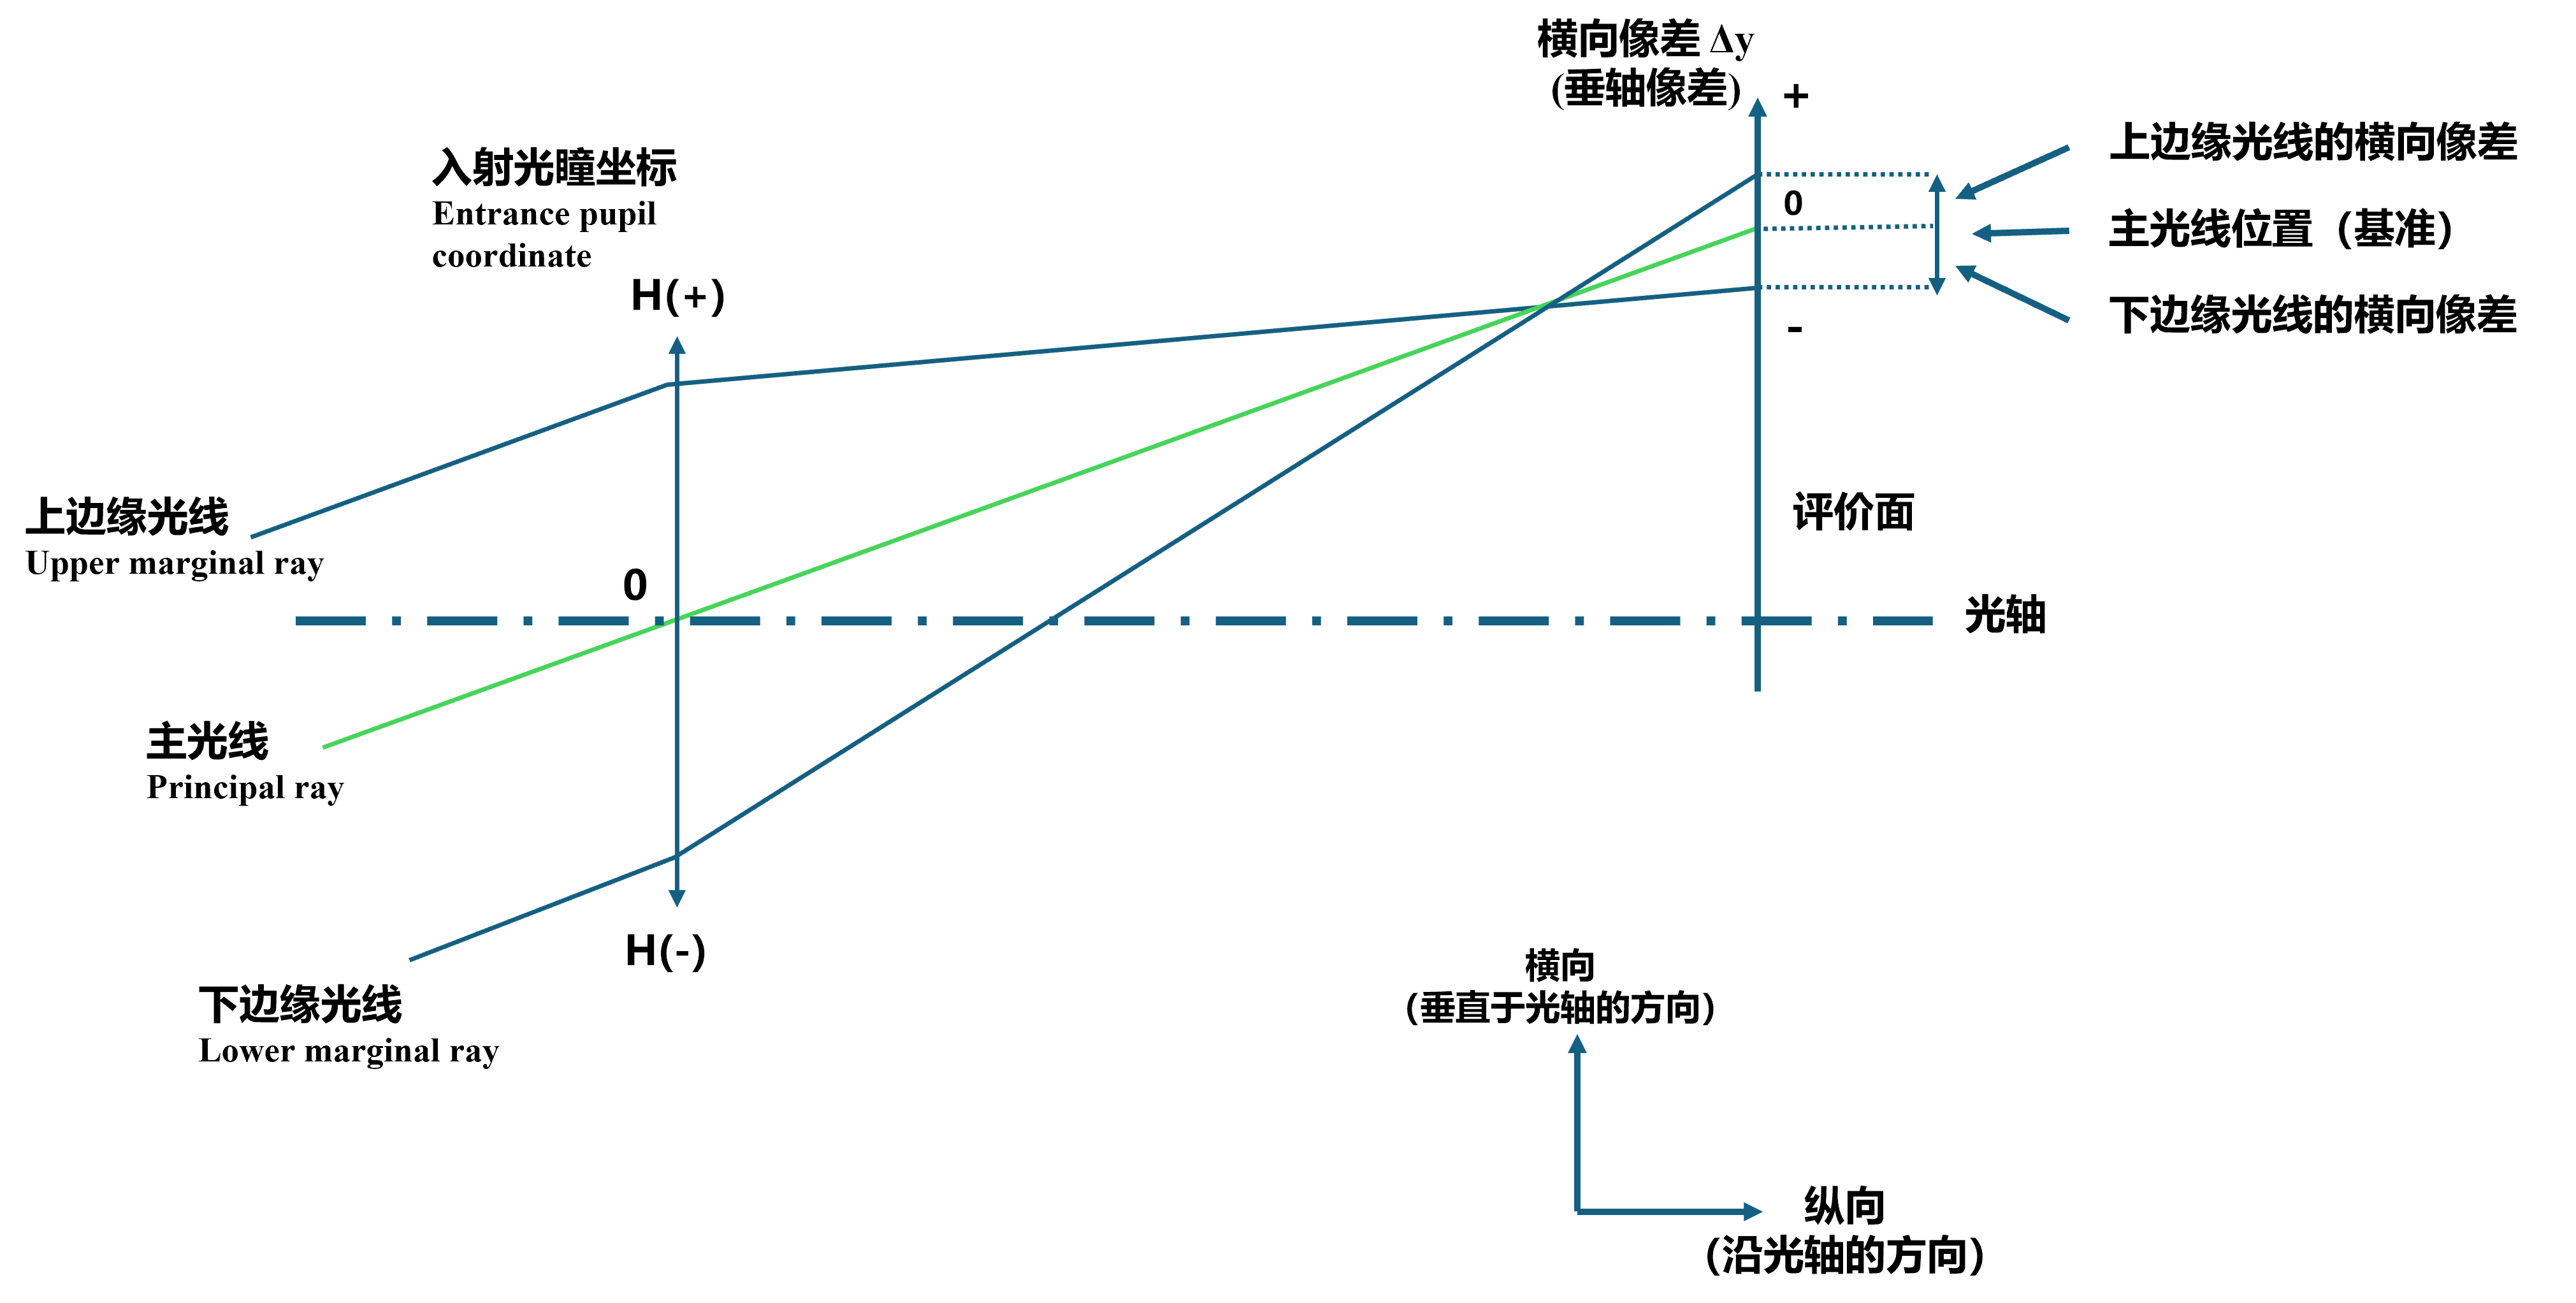
\includegraphics[width=\textwidth,height=.58\textheight,keepaspectratio]{Figure/图片1.png}
                \caption{光线穿过入瞳并落到评估面的几何关系}
                \label{fig:rayfan_ray_geometry_main}
            \end{figure}
        \end{column}
        \hfill
        \begin{column}{.50\textwidth}
            \begin{block}{Ray Fan 的读图方式}
                横轴是归一化入瞳坐标 $h\in[-1,1]$，纵轴是每条光线在评估面上的横向偏移，通常以主光线落点为原点。
            \end{block}

            \begin{itemize}
                \item \textbf{曲线斜率}：主要对应离焦、场曲、像散等线性项。
                \item \textbf{曲线弯曲}：对应球差、彗差等高阶项。
                \item \textbf{视场变化}：区分轴上像差和轴外像差。
                \item \textbf{波长变化}：区分单色像差和色差。
            \end{itemize}

            \alert{Ray Fan 是几何诊断图；PSF 是最终点像能量分布。两者相关，但不能混用图片和结论。}
        \end{column}
    \end{columns}
\end{frame}

\englishtitle{Ideal Imaging and Defocus}
\begin{frame}{理想成像与离焦}
\label{1.6}
    \begin{figure}
        \centering
        \begin{minipage}[t]{.32\textwidth}
            \centering
            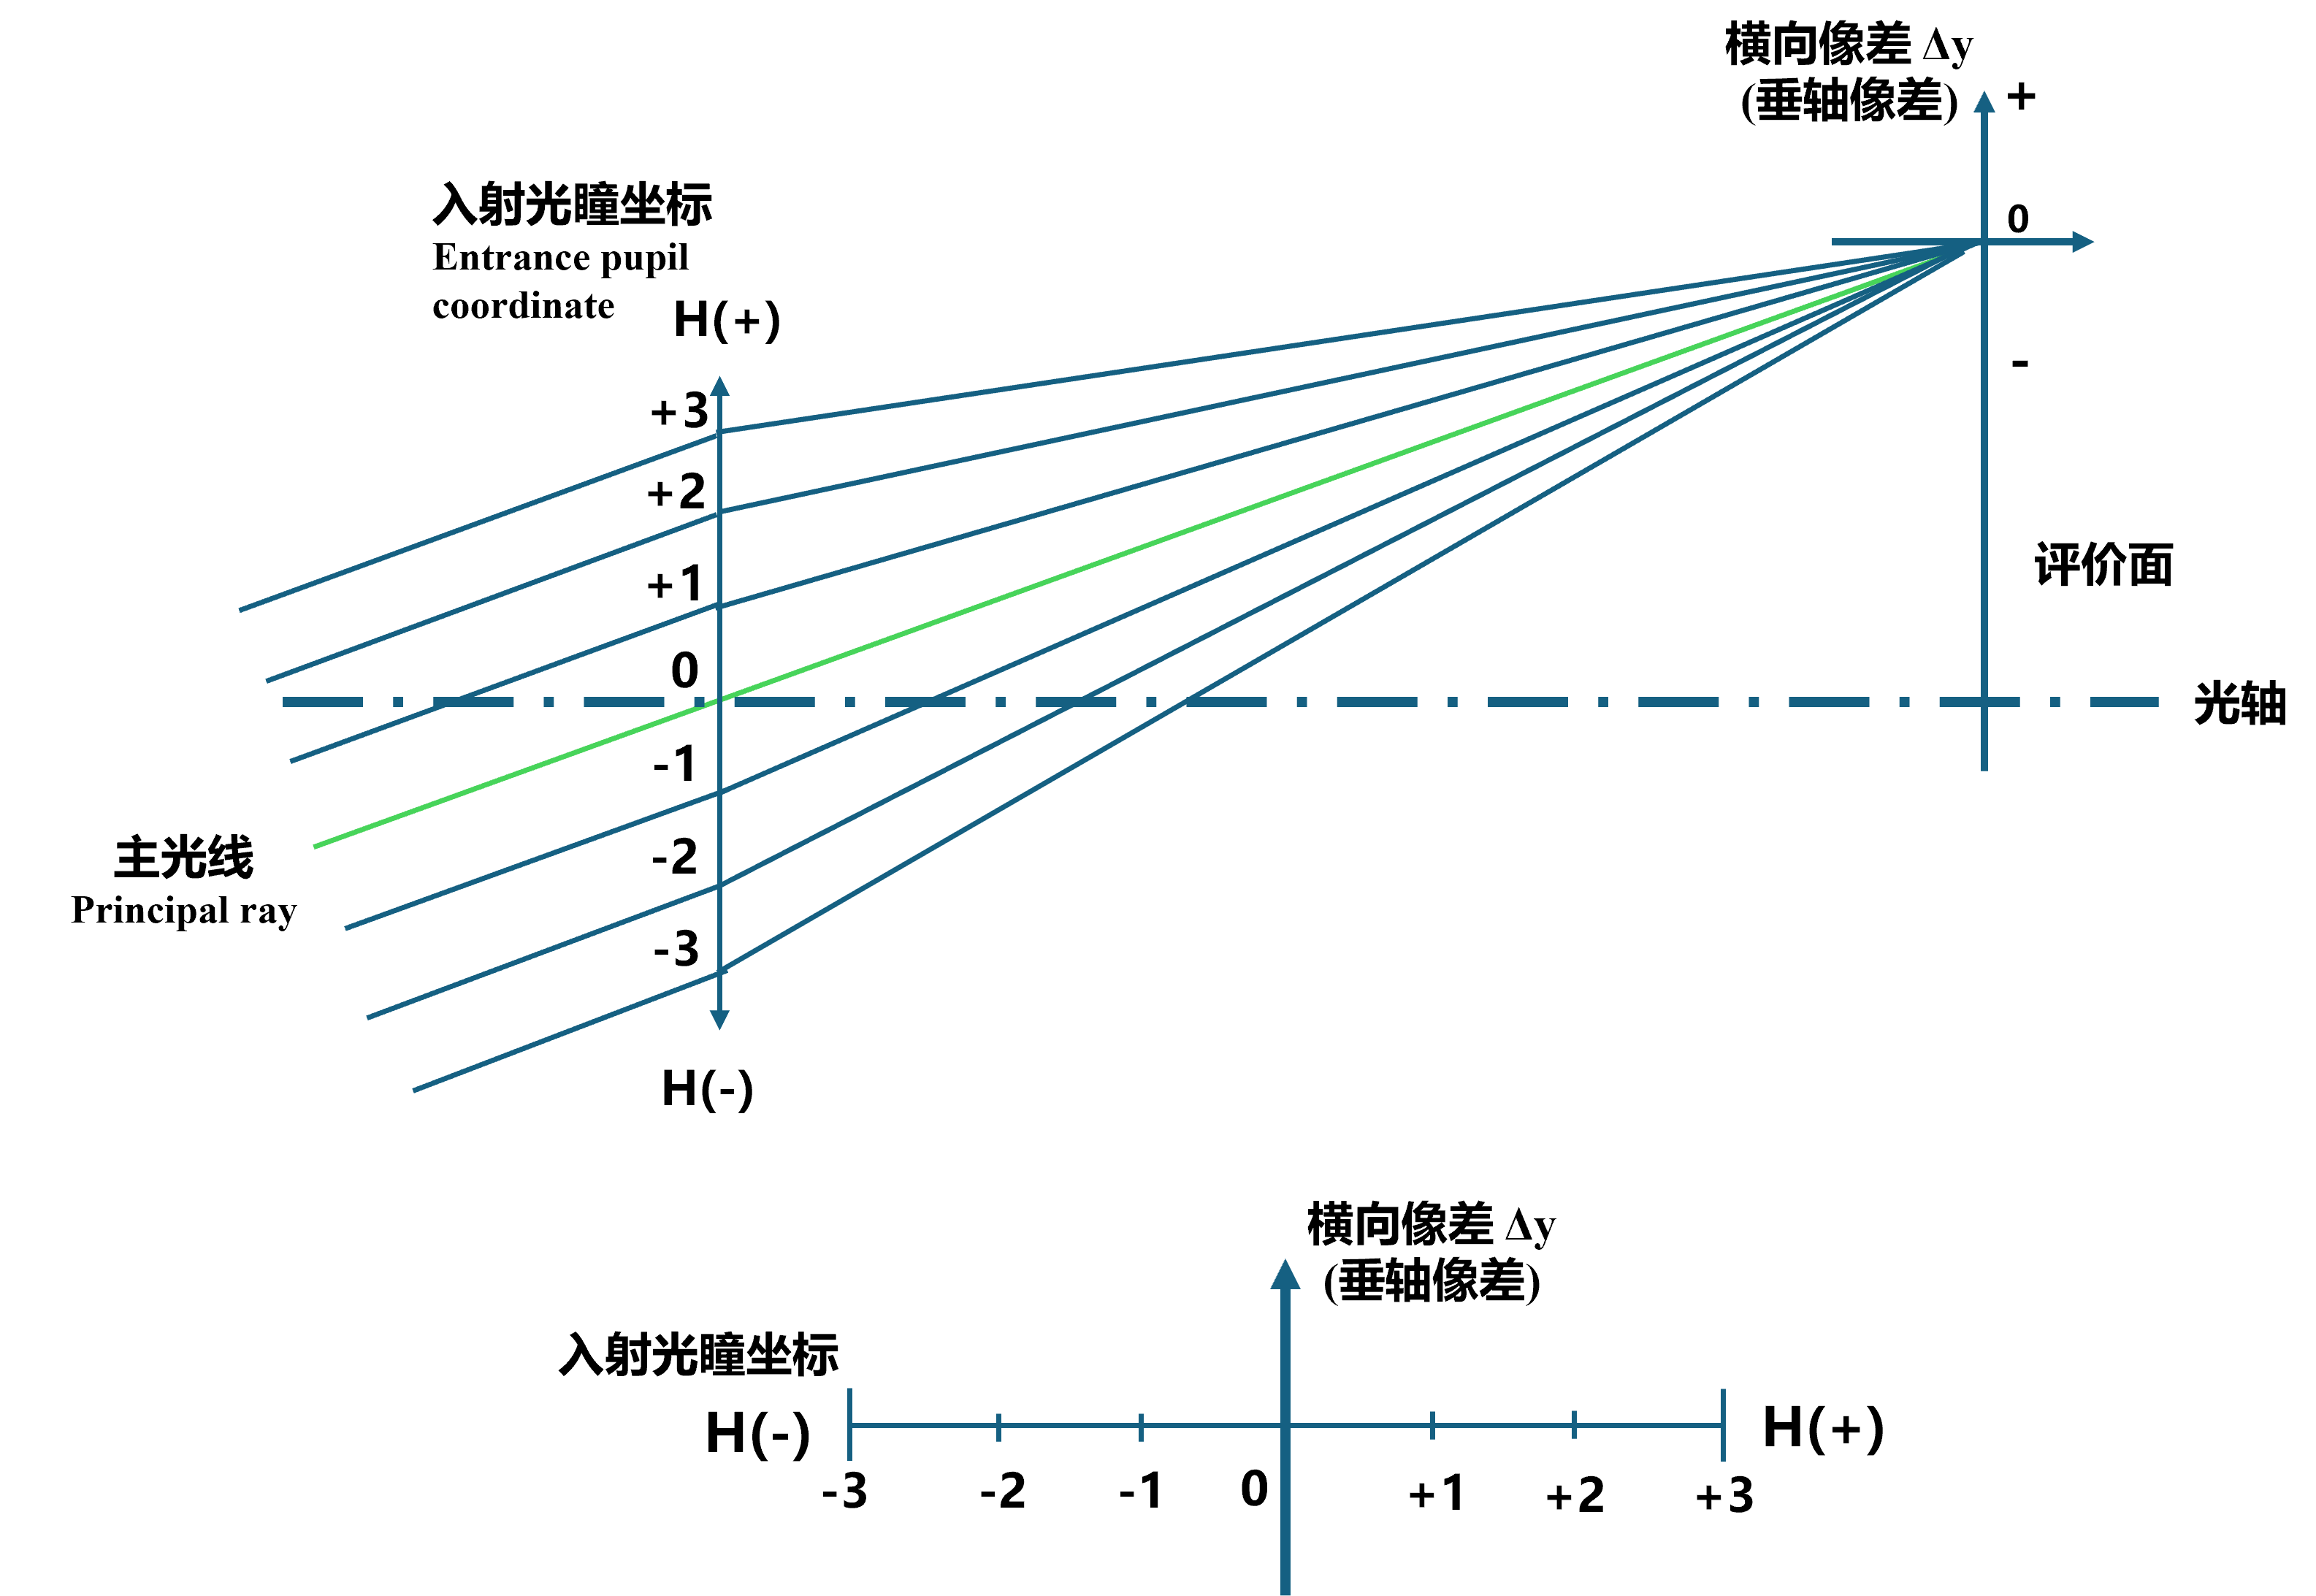
\includegraphics[width=\linewidth,height=.40\textheight,keepaspectratio]{Figure/图片3.png}
            \scriptsize 理想评估面：所有光线会聚于同一点
        \end{minipage}
        \hfill
        \begin{minipage}[t]{.32\textwidth}
            \centering
            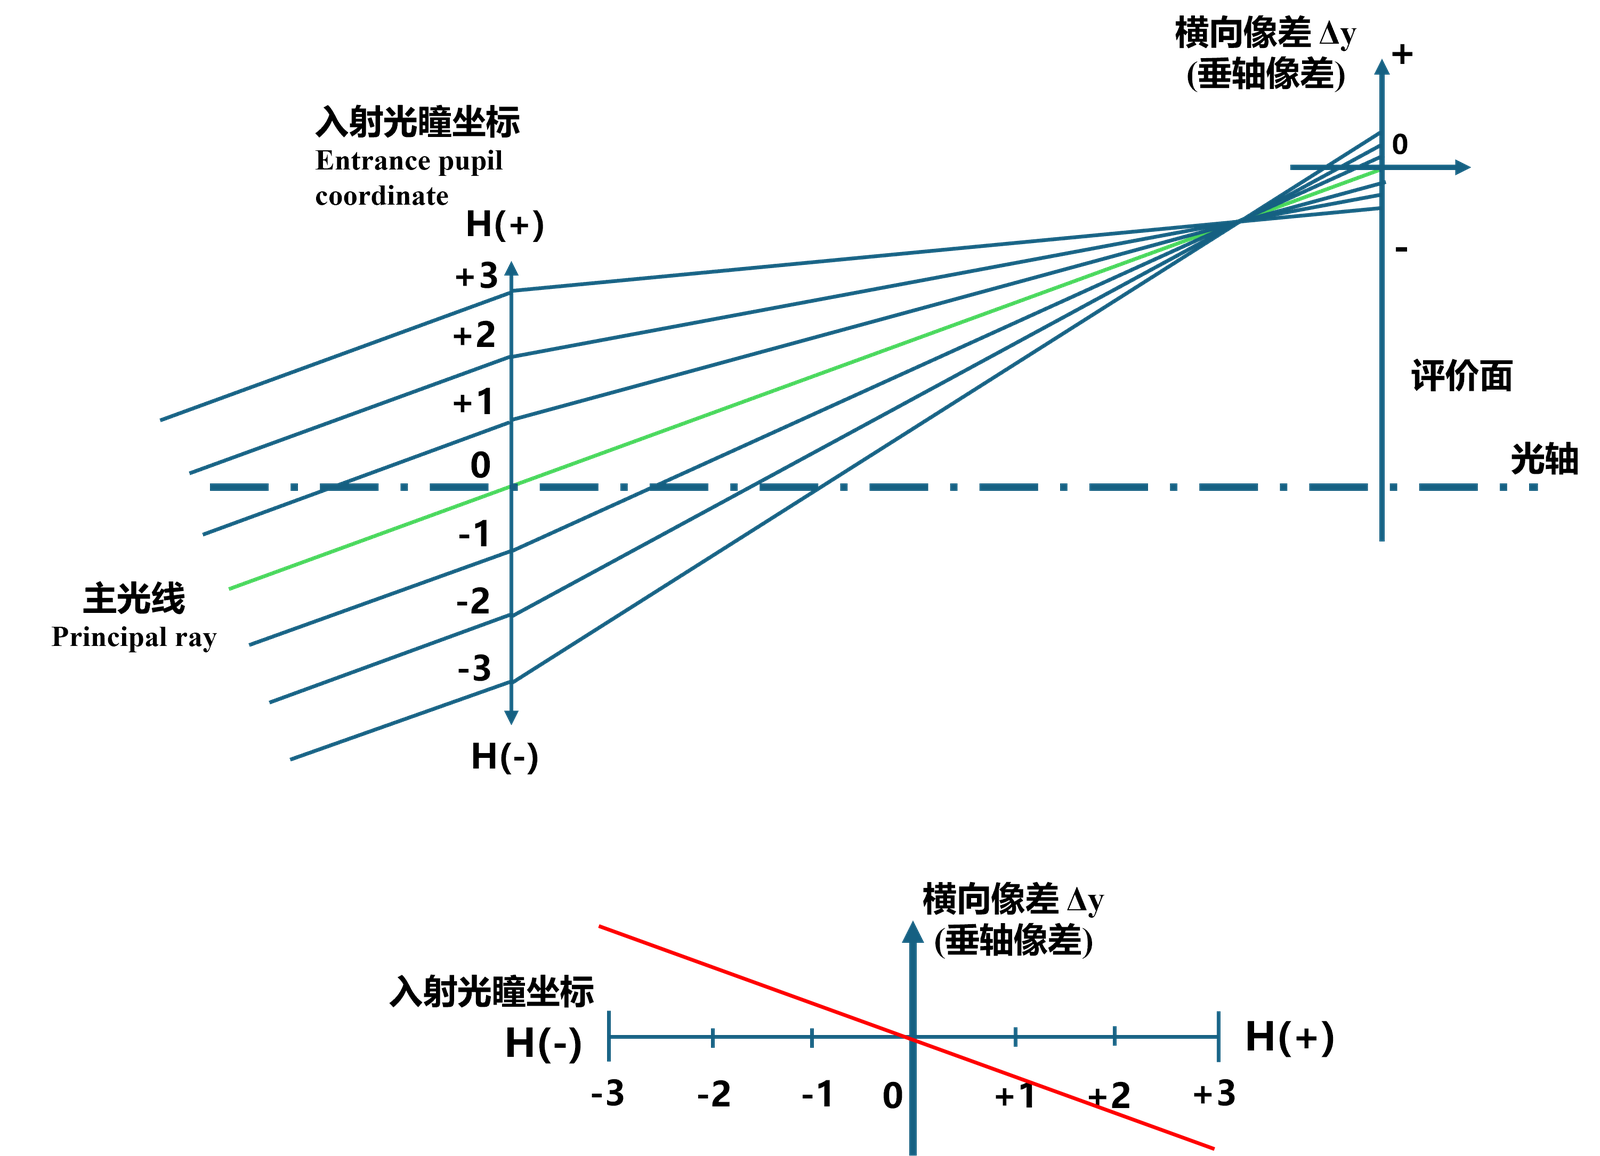
\includegraphics[width=\linewidth,height=.40\textheight,keepaspectratio]{Figure/图片4.png}
            \scriptsize 评估面远离最佳焦面：Ray Fan 呈一侧倾斜直线
        \end{minipage}
        \hfill
        \begin{minipage}[t]{.32\textwidth}
            \centering
            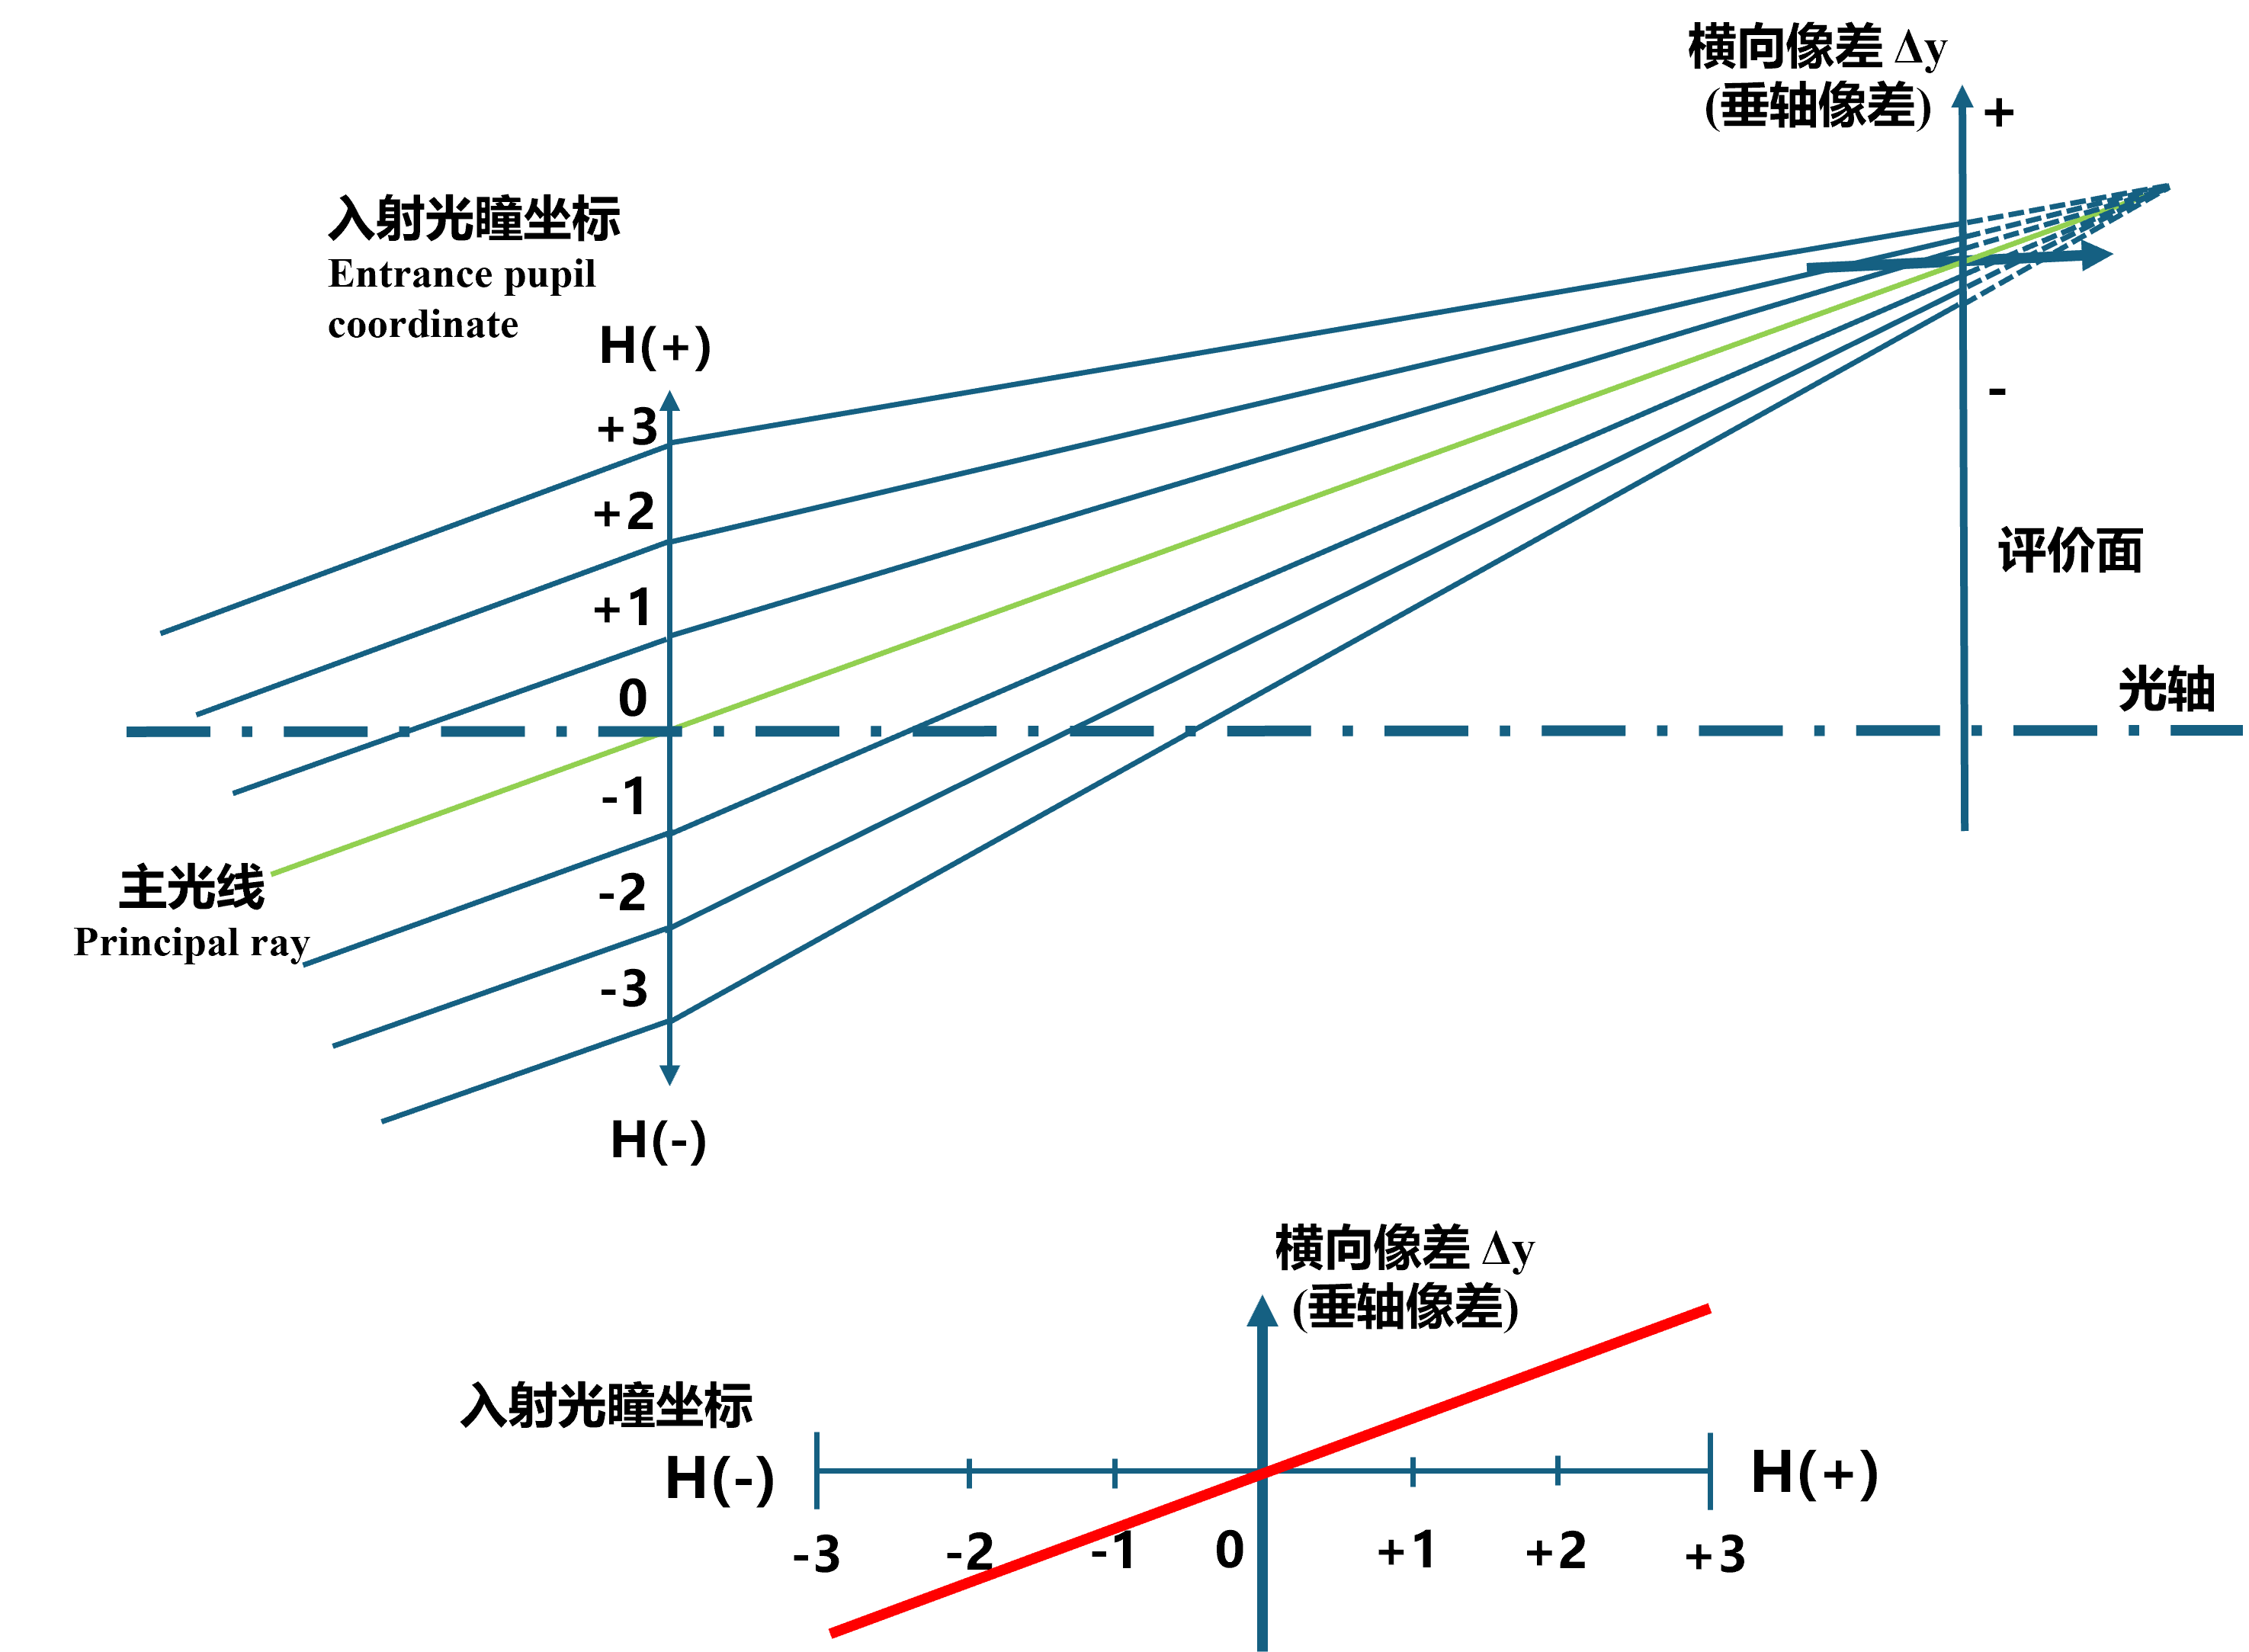
\includegraphics[width=\linewidth,height=.40\textheight,keepaspectratio]{Figure/图片6.png}
            \scriptsize 评估面靠近镜头：斜率方向相反
        \end{minipage}
        \caption{理想成像与正负离焦的统一示意}
        \label{fig:ideal_defocus_merged}
    \end{figure}

    \vspace{-4pt}
    \begin{columns}[T]
        \begin{column}{.50\textwidth}
            \begin{itemize}
                \item 无像差：横向像差为零，Ray Fan 落在横轴上。
                \item 离焦：Ray Fan 是通过原点的直线。
            \end{itemize}
        \end{column}
        \begin{column}{.50\textwidth}
            \begin{itemize}
                \item 改变像面位置只能消除线性离焦项。
                \item 弯曲项仍存在时，需要改变光学结构或面形。
            \end{itemize}
        \end{column}
    \end{columns}
\end{frame}

\subsection{Seidel 像差与 Zernike 展开}
\label{sec:1.3}

\englishtitle{Third-Order Aberration as Residual After Paraxial Imaging}
\begin{frame}{三阶像差：理想成像之后的最低阶残差}
\label{1.7}
    \small
    \textbf{在一阶成像已经确定之后，Ray Fan 的最低阶残差可写成：}
    \begin{equation}
        \Delta y(h,\omega)
        \approx A h
        + B h^3
        + C h^2\tan\omega
        + D h\tan^2\omega
        + E\tan^3\omega
        \label{eq:rayfan_third_order}
    \end{equation}

    \vspace{-2pt}
    \begin{table}
        \centering
        \scriptsize
        \renewcommand{\arraystretch}{1.25}
        \begin{tabular}{p{2.1cm}|p{2.2cm}|p{2.5cm}|p{4.5cm}}
            \toprule
            \textbf{项} & \textbf{孔径依赖} & \textbf{视场依赖} & \textbf{Ray Fan 诊断特征} \\
            \midrule
            离焦 & $h$ & 与视场弱相关 & 通过原点的直线，移动像面可改变斜率 \\
            球差 & $h^3$ & 轴上存在 & 奇函数三次曲线，边缘孔径贡献最大 \\
            彗差 & $h^2$ & $\tan\omega$ & 偶函数二次曲线，离轴视场快速变坏 \\
            像散/场曲 & $h$ & $\tan^2\omega$ & 原点附近斜率随视场或子午/弧矢方向改变 \\
            畸变 & $h^0$ & $\tan^3\omega$ & 主光线像高偏移，Ray Fan 不直接显示弥散形状 \\
            \bottomrule
        \end{tabular}
        \caption{三阶项与横向像差图的对应关系}
        \label{tab:third_order_rayfan_main}
    \end{table}

    \alert{合并后的理解：}一阶量负责把像“放到正确位置”；三阶项描述“放到那里之后还剩下什么形状的误差”。
\end{frame}

\englishtitle{Zernike Polynomial Expansion}
\begin{frame}{Zernike 多项式：波前像差的正交坐标系}
\label{1.8}
    \begin{columns}[T]
        \begin{column}{.52\textwidth}
            对圆形光瞳，波像差通常展开为：
            \begin{equation}
                W(\rho,\theta)=\sum_j C_j Z_j(\rho,\theta),
                \qquad 0\le \rho \le 1
                \label{eq:zernike_main}
            \end{equation}

            \begin{equation}
                Z_n^m(\rho,\theta)
                =R_n^m(\rho)\cos(m\theta)
                \ \text{或}\
                R_n^m(\rho)\sin(m\theta)
                \label{eq:zernike_nm_main}
            \end{equation}

            \begin{equation}
                \int_0^1\!\!\int_0^{2\pi}
                Z_i Z_j\,\rho\,d\theta\,d\rho
                = N_i\delta_{ij}
                \label{eq:zernike_orthogonal_main}
            \end{equation}
        \end{column}
        \hfill
        \begin{column}{.48\textwidth}
            \begin{itemize}
                \item Zernike直接面向\alert{波前 $W$}，比单纯看 Ray Fan 更接近像质根源。
                \item 正交性让每个系数 $C_j$ 具有相对独立的含义，便于量化比较。
                \item Zemax 的 Wavefront Map、Zernike Standard Coefficients 和 RMS Wavefront 都建立在同一套波前语言上。
                \item 干涉仪测量、自由曲面补偿和自适应光学校正也常用 Zernike 系数沟通。
            \end{itemize}

            \begin{alertblock}{从波前到光线}
                Ray Fan 可近似理解为波前斜率的表现：
                \[
                    \Delta \mathbf{r}_{\perp}\propto \nabla_{\rho,\theta} W
                \]
            \end{alertblock}
        \end{column}
    \end{columns}
\end{frame}

\englishtitle{Zernike Modes and Physical Aberrations}
\begin{frame}{常用 Zernike 模式与像差含义}
\label{1.9}
    \scriptsize
    \begin{table}
        \centering
        \renewcommand{\arraystretch}{1.42}
        \begin{tabular}{p{2.3cm}|p{3.2cm}|p{3.0cm}|p{3.4cm}}
            \toprule
            \textbf{Zernike 模式} & \textbf{典型形式} & \textbf{物理含义} & \textbf{诊断用途} \\
            \midrule
            Piston & $1$ & 整体相位常数 & 不影响成像，通常去除 \\
            Tilt X/Y & $\rho\cos\theta,\ \rho\sin\theta$ & 像点平移或装调倾斜 & 通常作为对准误差处理 \\
            Defocus & $2\rho^2-1$ & 像面前后移动 & 与 Ray Fan 直线斜率对应 \\
            Astigmatism & $\rho^2\cos2\theta,\ \rho^2\sin2\theta$ & 两个正交方向焦点不同 & 区分子午与弧矢焦面 \\
            Coma & $(3\rho^3-2\rho)\cos\theta$ 等 & 轴外不对称波前 & 对应 Ray Fan 二次弯曲 \\
            Primary spherical & $6\rho^4-6\rho^2+1$ & 边缘与近轴光线焦点不同 & 对应轴上三次型 Ray Fan \\
            Higher order terms & $n\ge5$ & 高阶球差、二级彗差等 & 大 NA、自由曲面或复杂系统中需关注 \\
            \bottomrule
        \end{tabular}
        \caption{Zernike 系数不是装饰性输出，而是可用于优化、测量和误差分解的波前坐标}
        \label{tab:zernike_modes_main}
    \end{table}

    \vspace{-2pt}
    \begin{block}{使用建议}
        先移除 piston、tilt 和必要的 defocus，再讨论剩余 Zernike 系数；否则装调误差和像面位置会掩盖真正的设计像差。
    \end{block}
\end{frame}

\subsection{单色像差诊断：先分清曲线形状}
\label{sec:1.4}

\englishtitle{Monochromatic Aberrations in Ray Fan}
\begin{frame}{球差、彗差与离焦：先看曲线阶次}
\label{1.10}
    \begin{figure}
        \centering
        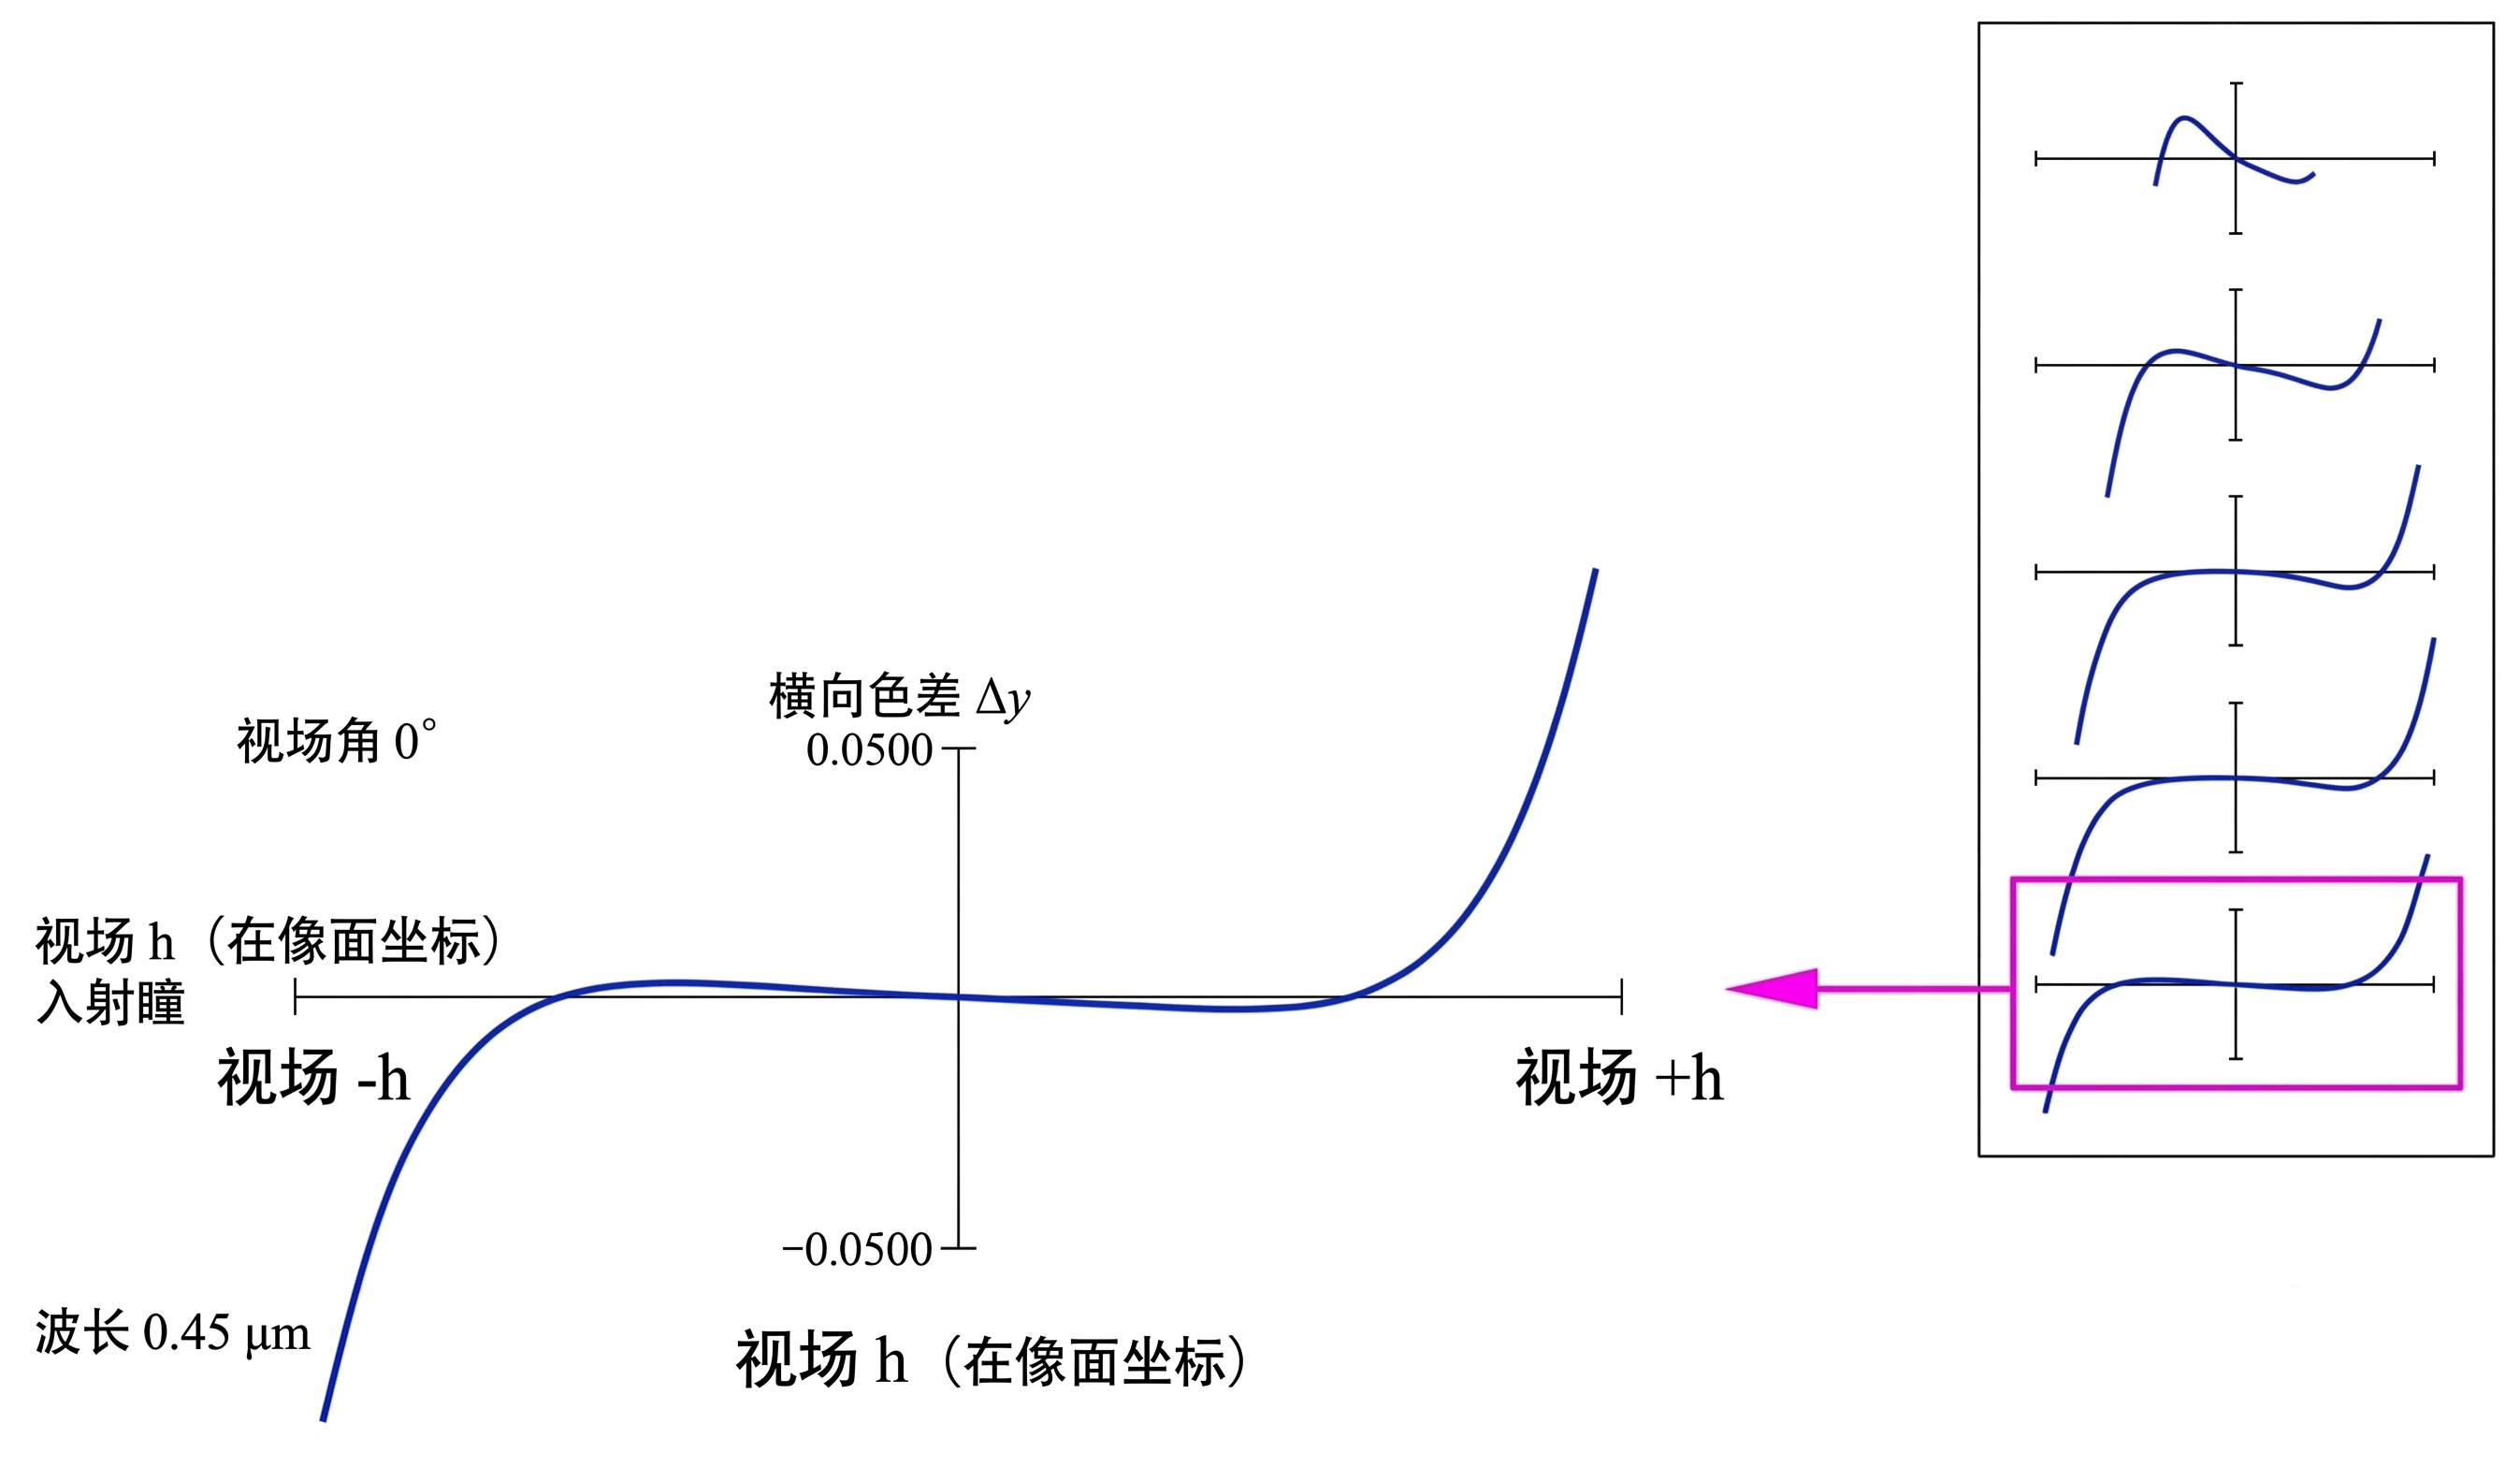
\includegraphics[width=.48\textwidth,height=.28\textheight,keepaspectratio]{Figure/图片23.png}\hfill
        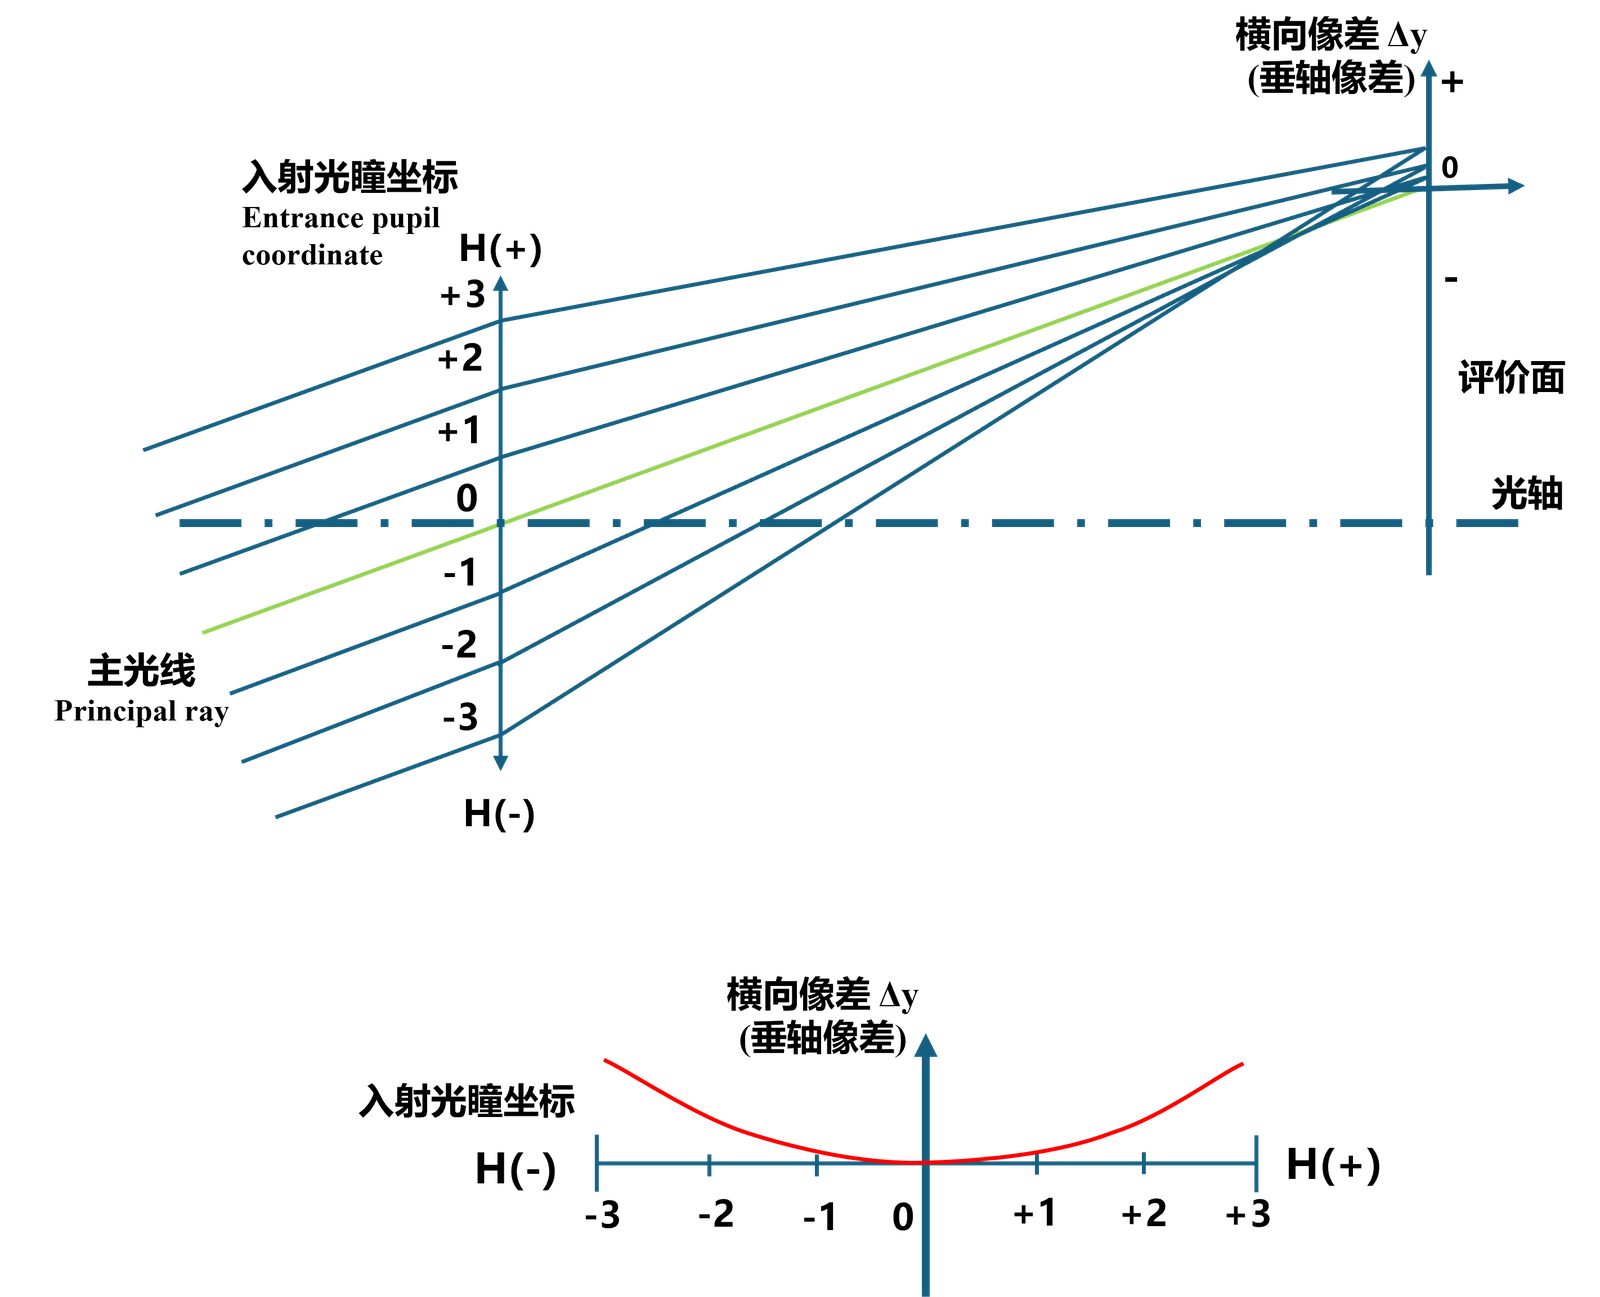
\includegraphics[width=.23\textwidth,height=.20\textheight,keepaspectratio]{Figure/图片8.png}\hfill
        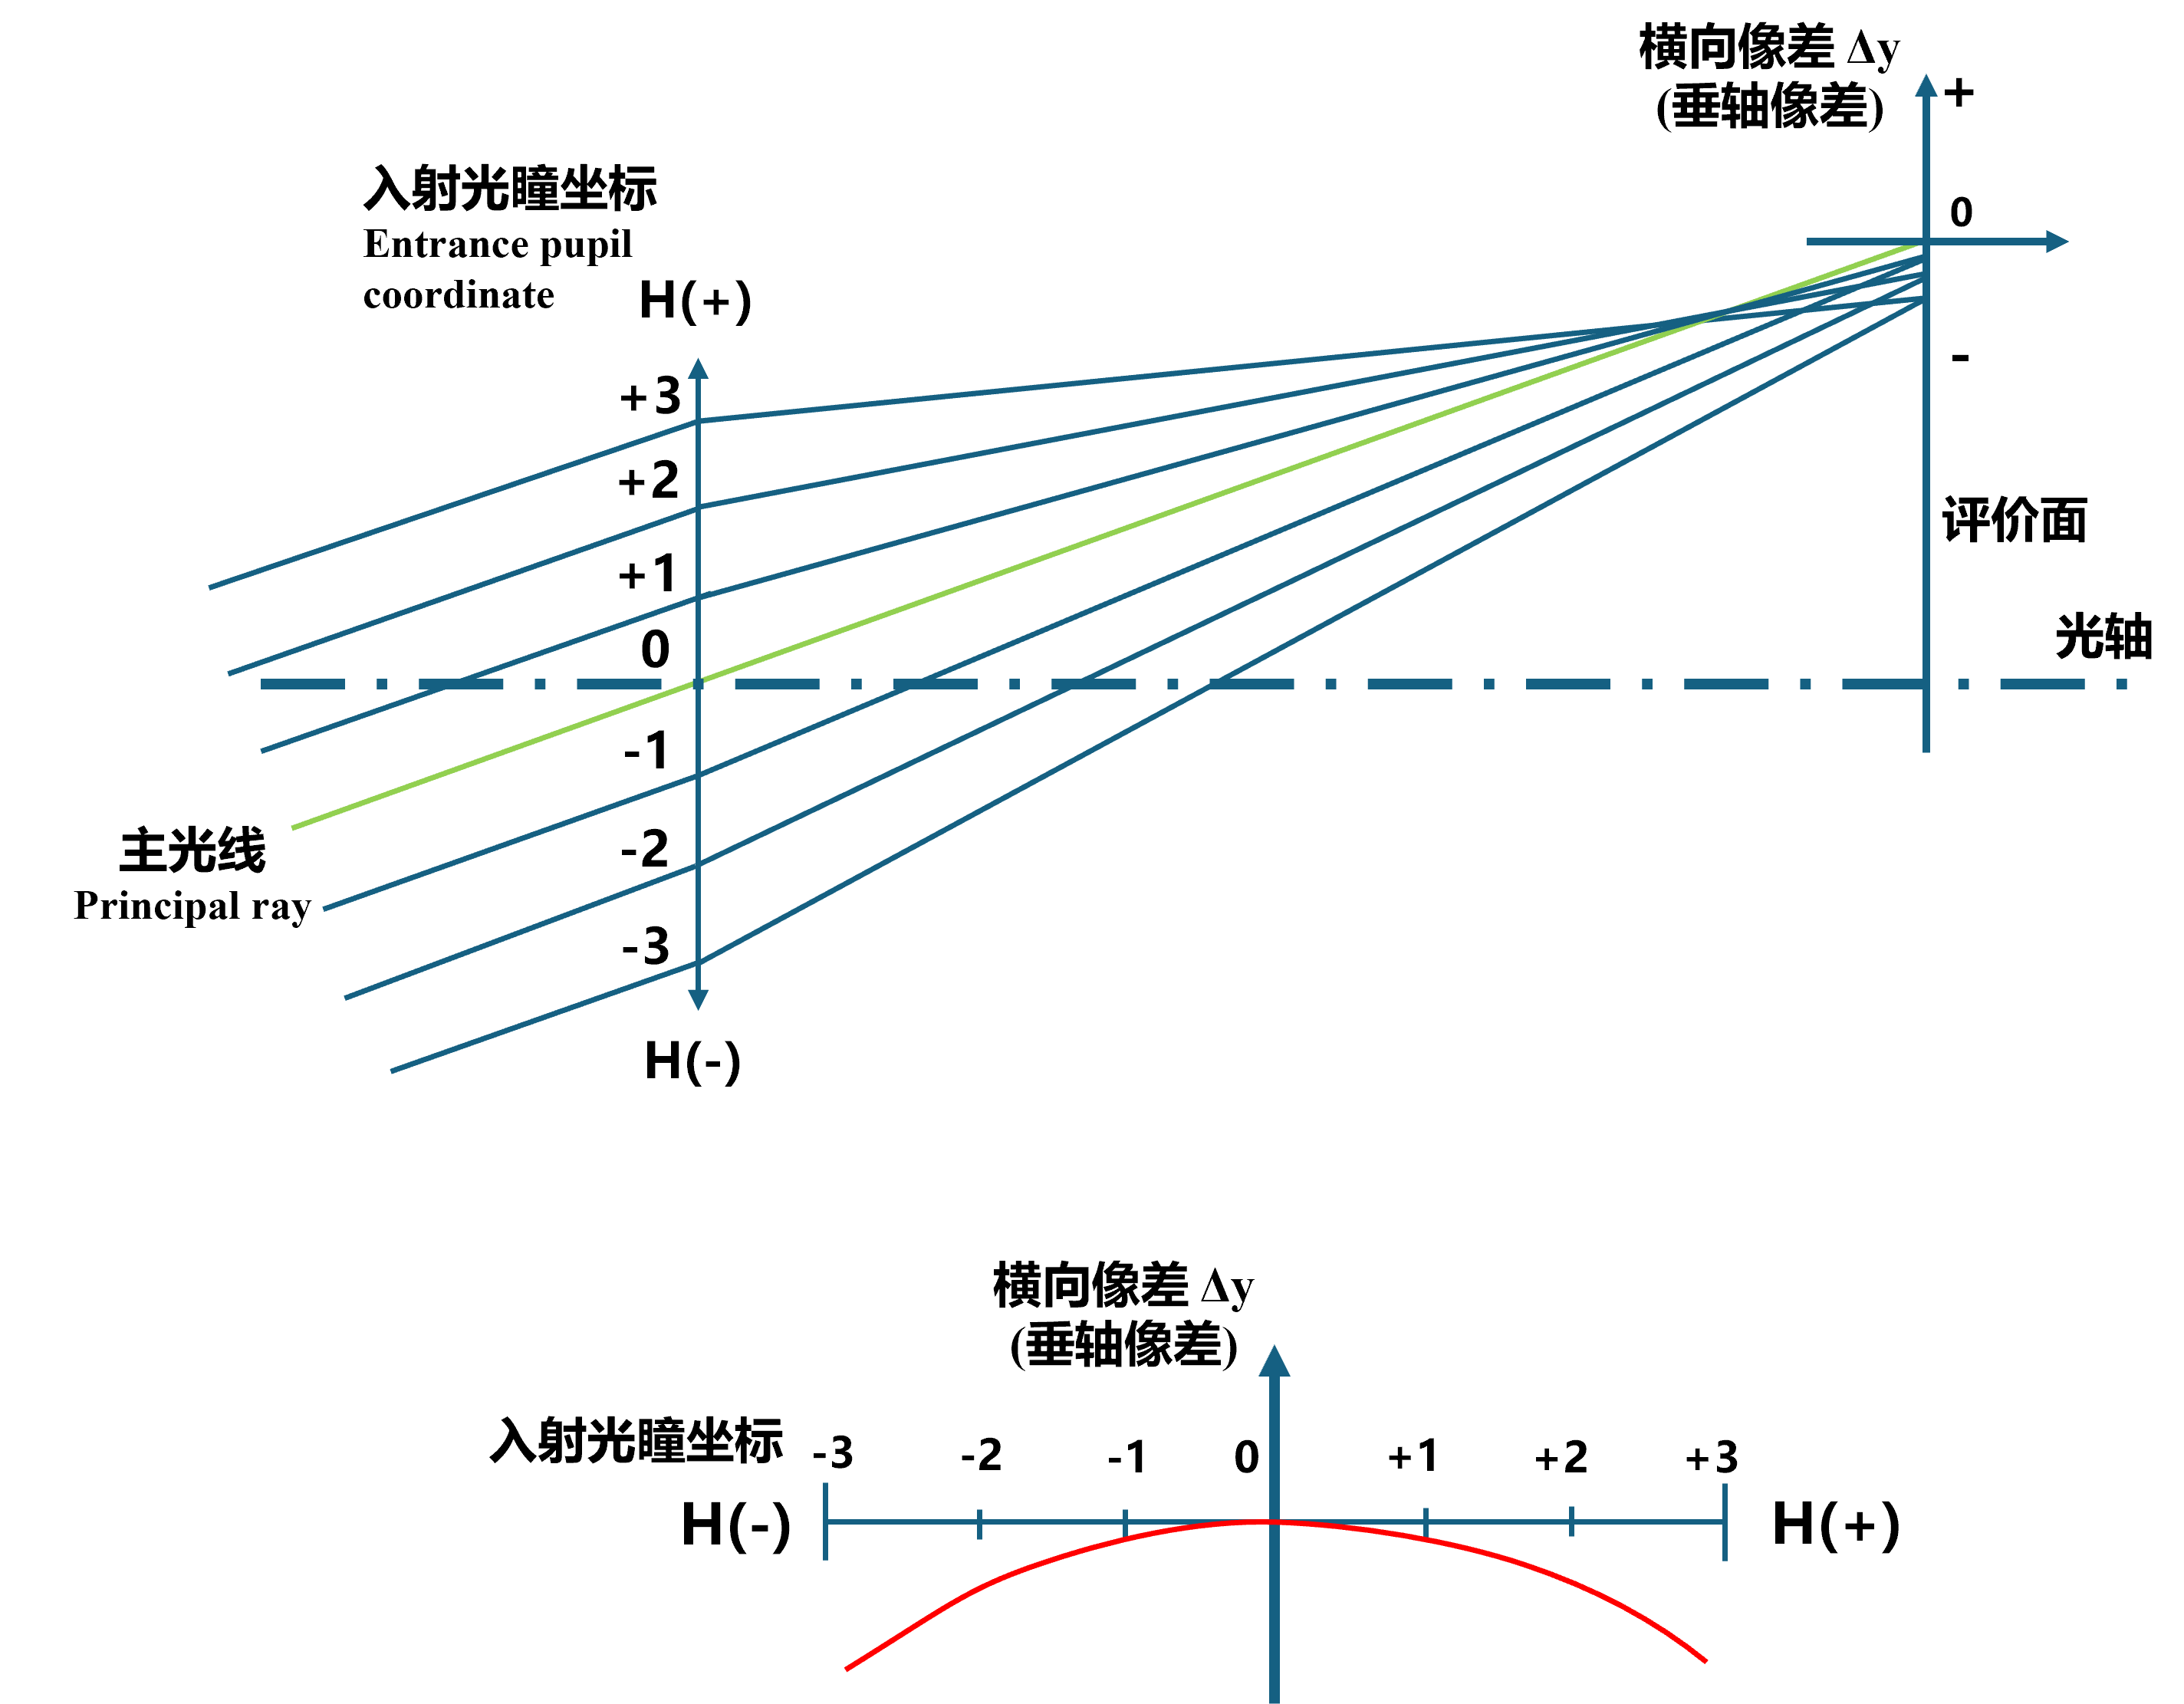
\includegraphics[width=.23\textwidth,height=.20\textheight,keepaspectratio]{Figure/图片11.png}
        \caption{左：球差的三次型 Ray Fan；右：彗差的二次型 Ray Fan，开口方向区分内向/外向}
        \label{fig:spherical_coma_rayfan_main}
    \end{figure}

    \vspace{-4pt}
    \begin{table}
        \centering
        \scriptsize
        \renewcommand{\arraystretch}{1.3}
        \begin{tabular}{p{1.8cm}|p{3.2cm}|p{4.8cm}}
            \toprule
            \textbf{类型} & \textbf{Ray Fan 特征} & \textbf{设计动作} \\
            \midrule
            离焦 & 通过原点的直线 & 先移动像面；若只剩斜率，优先修焦面位置 \\
            球差 & 轴上三次曲线，边缘孔径贡献最大 & 分摊光焦度、改变弯曲因子、引入非球面 \\
            彗差 & 离轴二次曲线，随视场快速增加 & 调整光阑位置、增强结构对称性、降低离轴入射角 \\
            \bottomrule
        \end{tabular}
    \end{table}

    \alert{这一页把原先分散的离焦、球差、彗差合并为一个判据：先看阶次，再决定是移像面还是改结构。}
\end{frame}

\englishtitle{Field Curvature and Astigmatism}
\begin{frame}{场曲与像散：同是斜率问题，但物理来源不同}
\label{1.11}
    \begin{columns}[T]
        \begin{column}{.53\textwidth}
            \begin{figure}
                \centering
                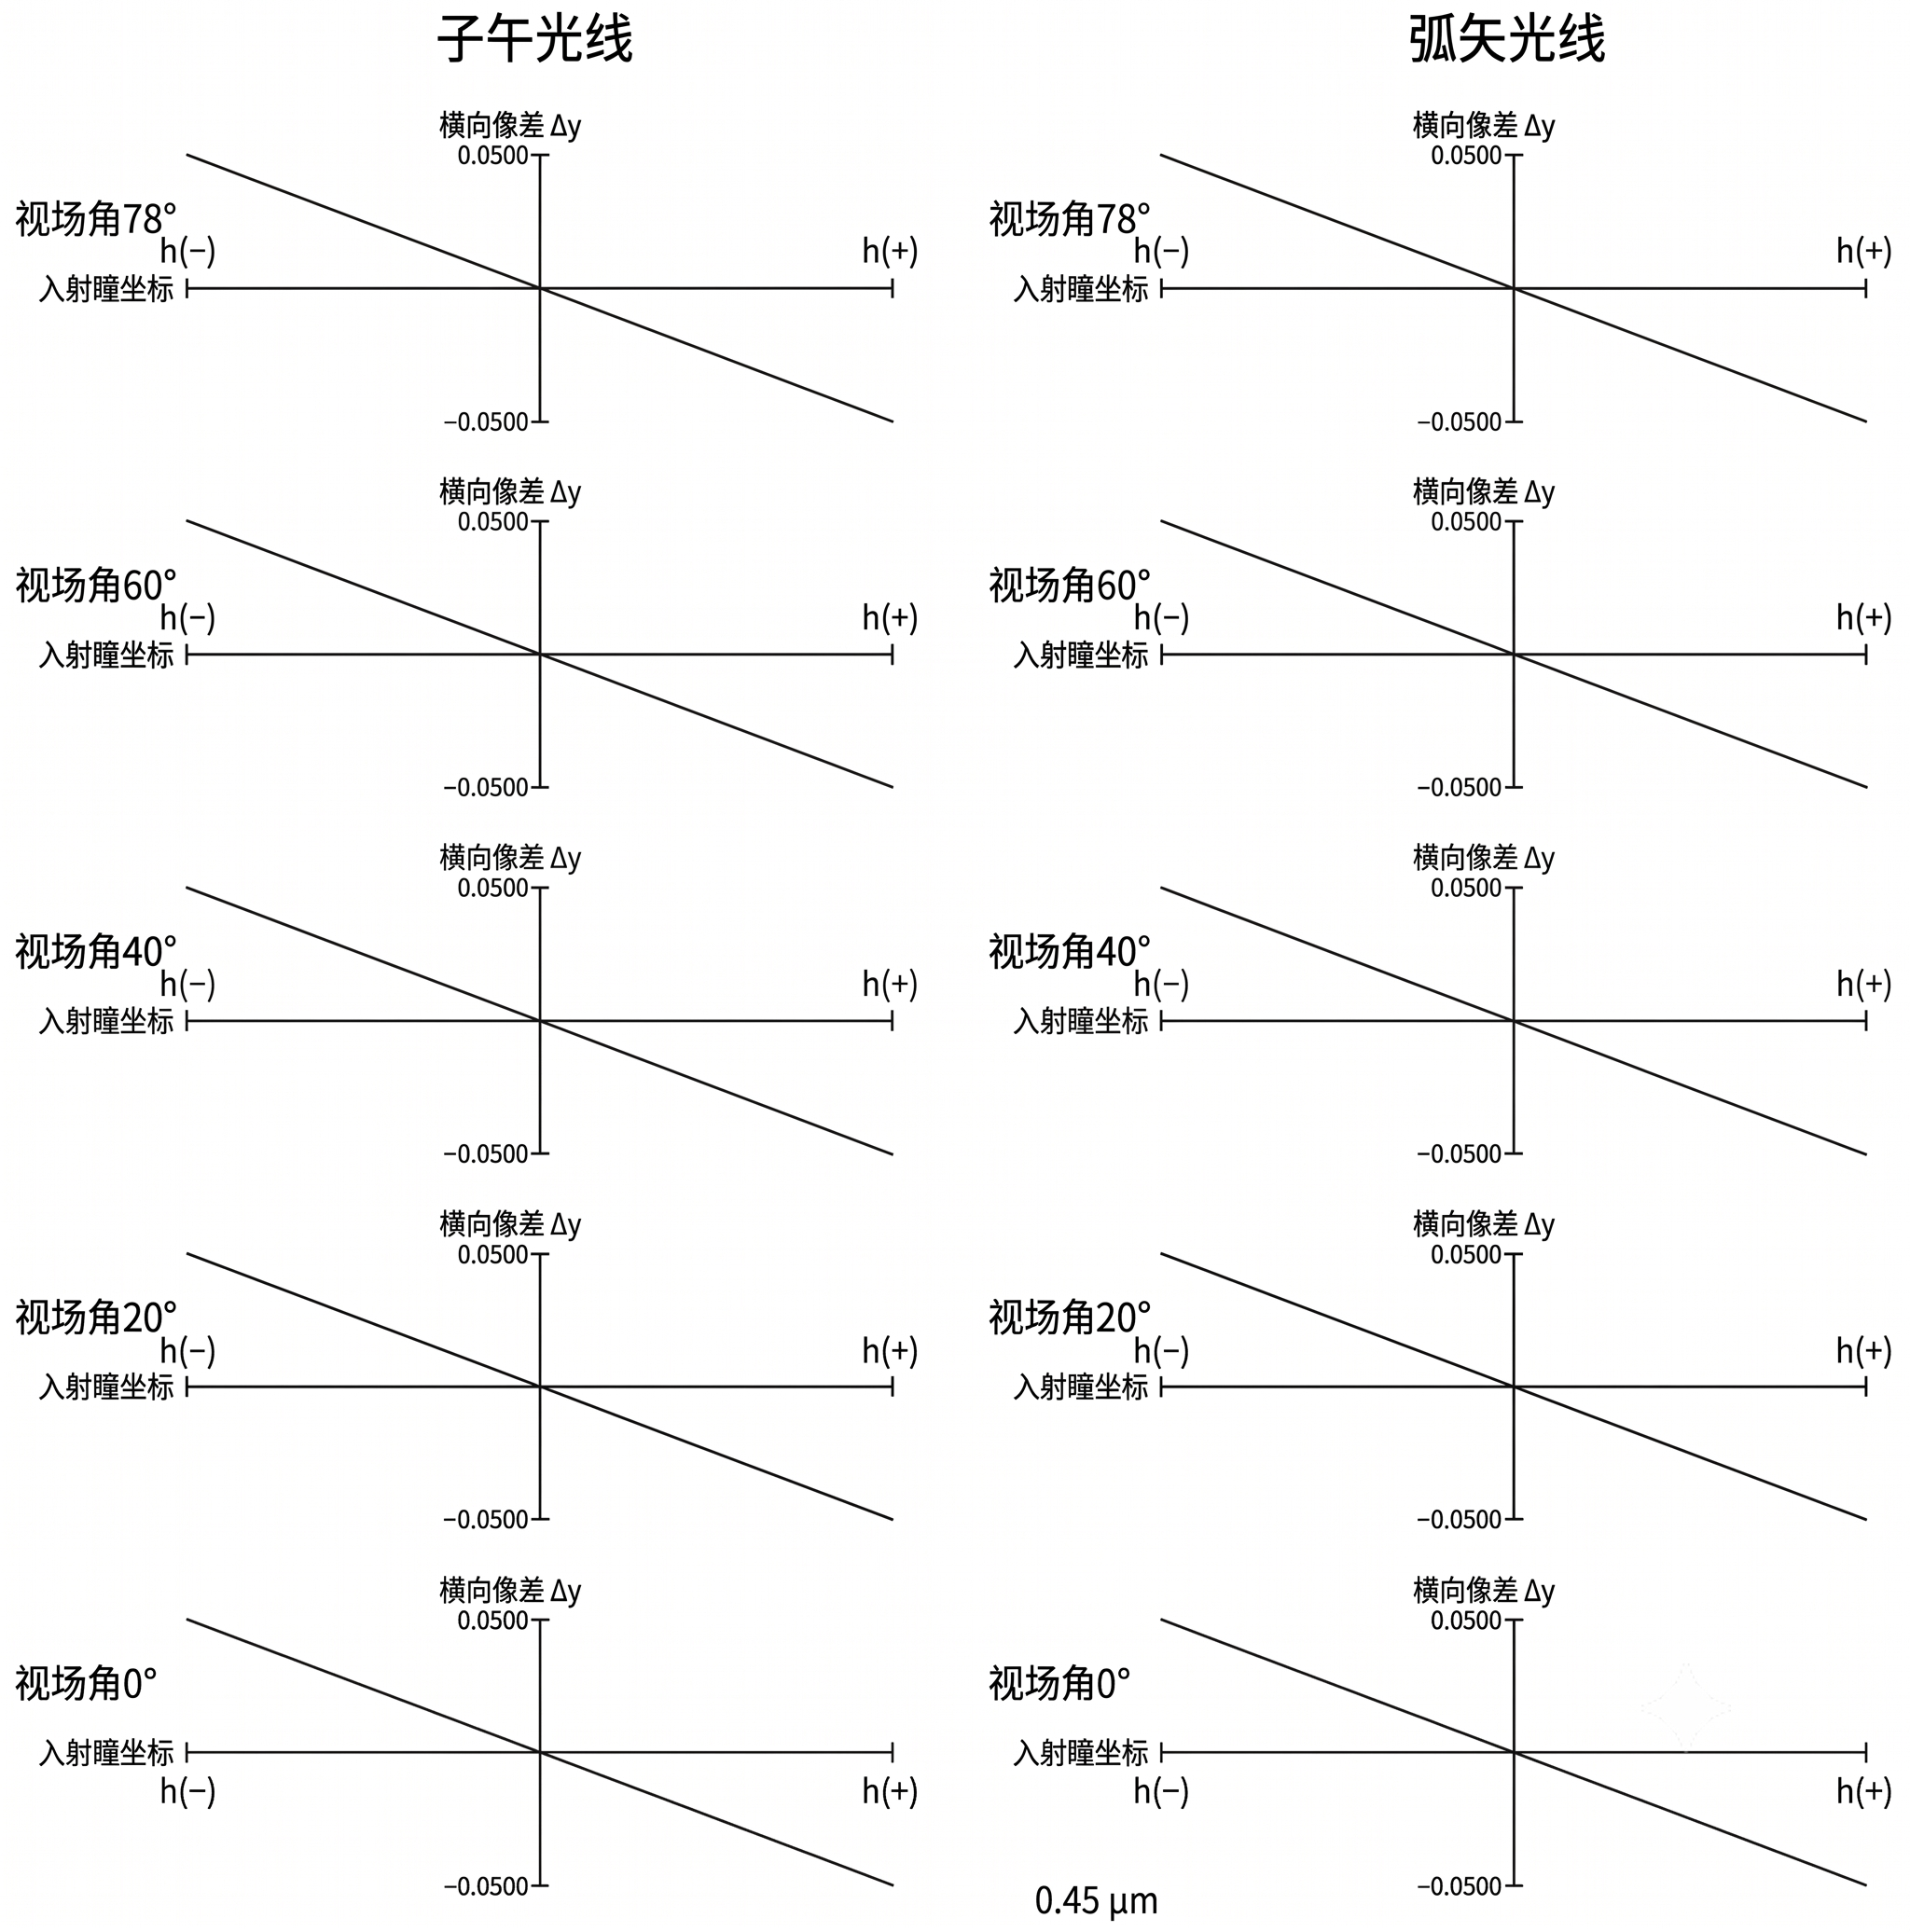
\includegraphics[width=.32\textwidth,height=.25\textheight,keepaspectratio]{Figure/图片20.png}\hfill
                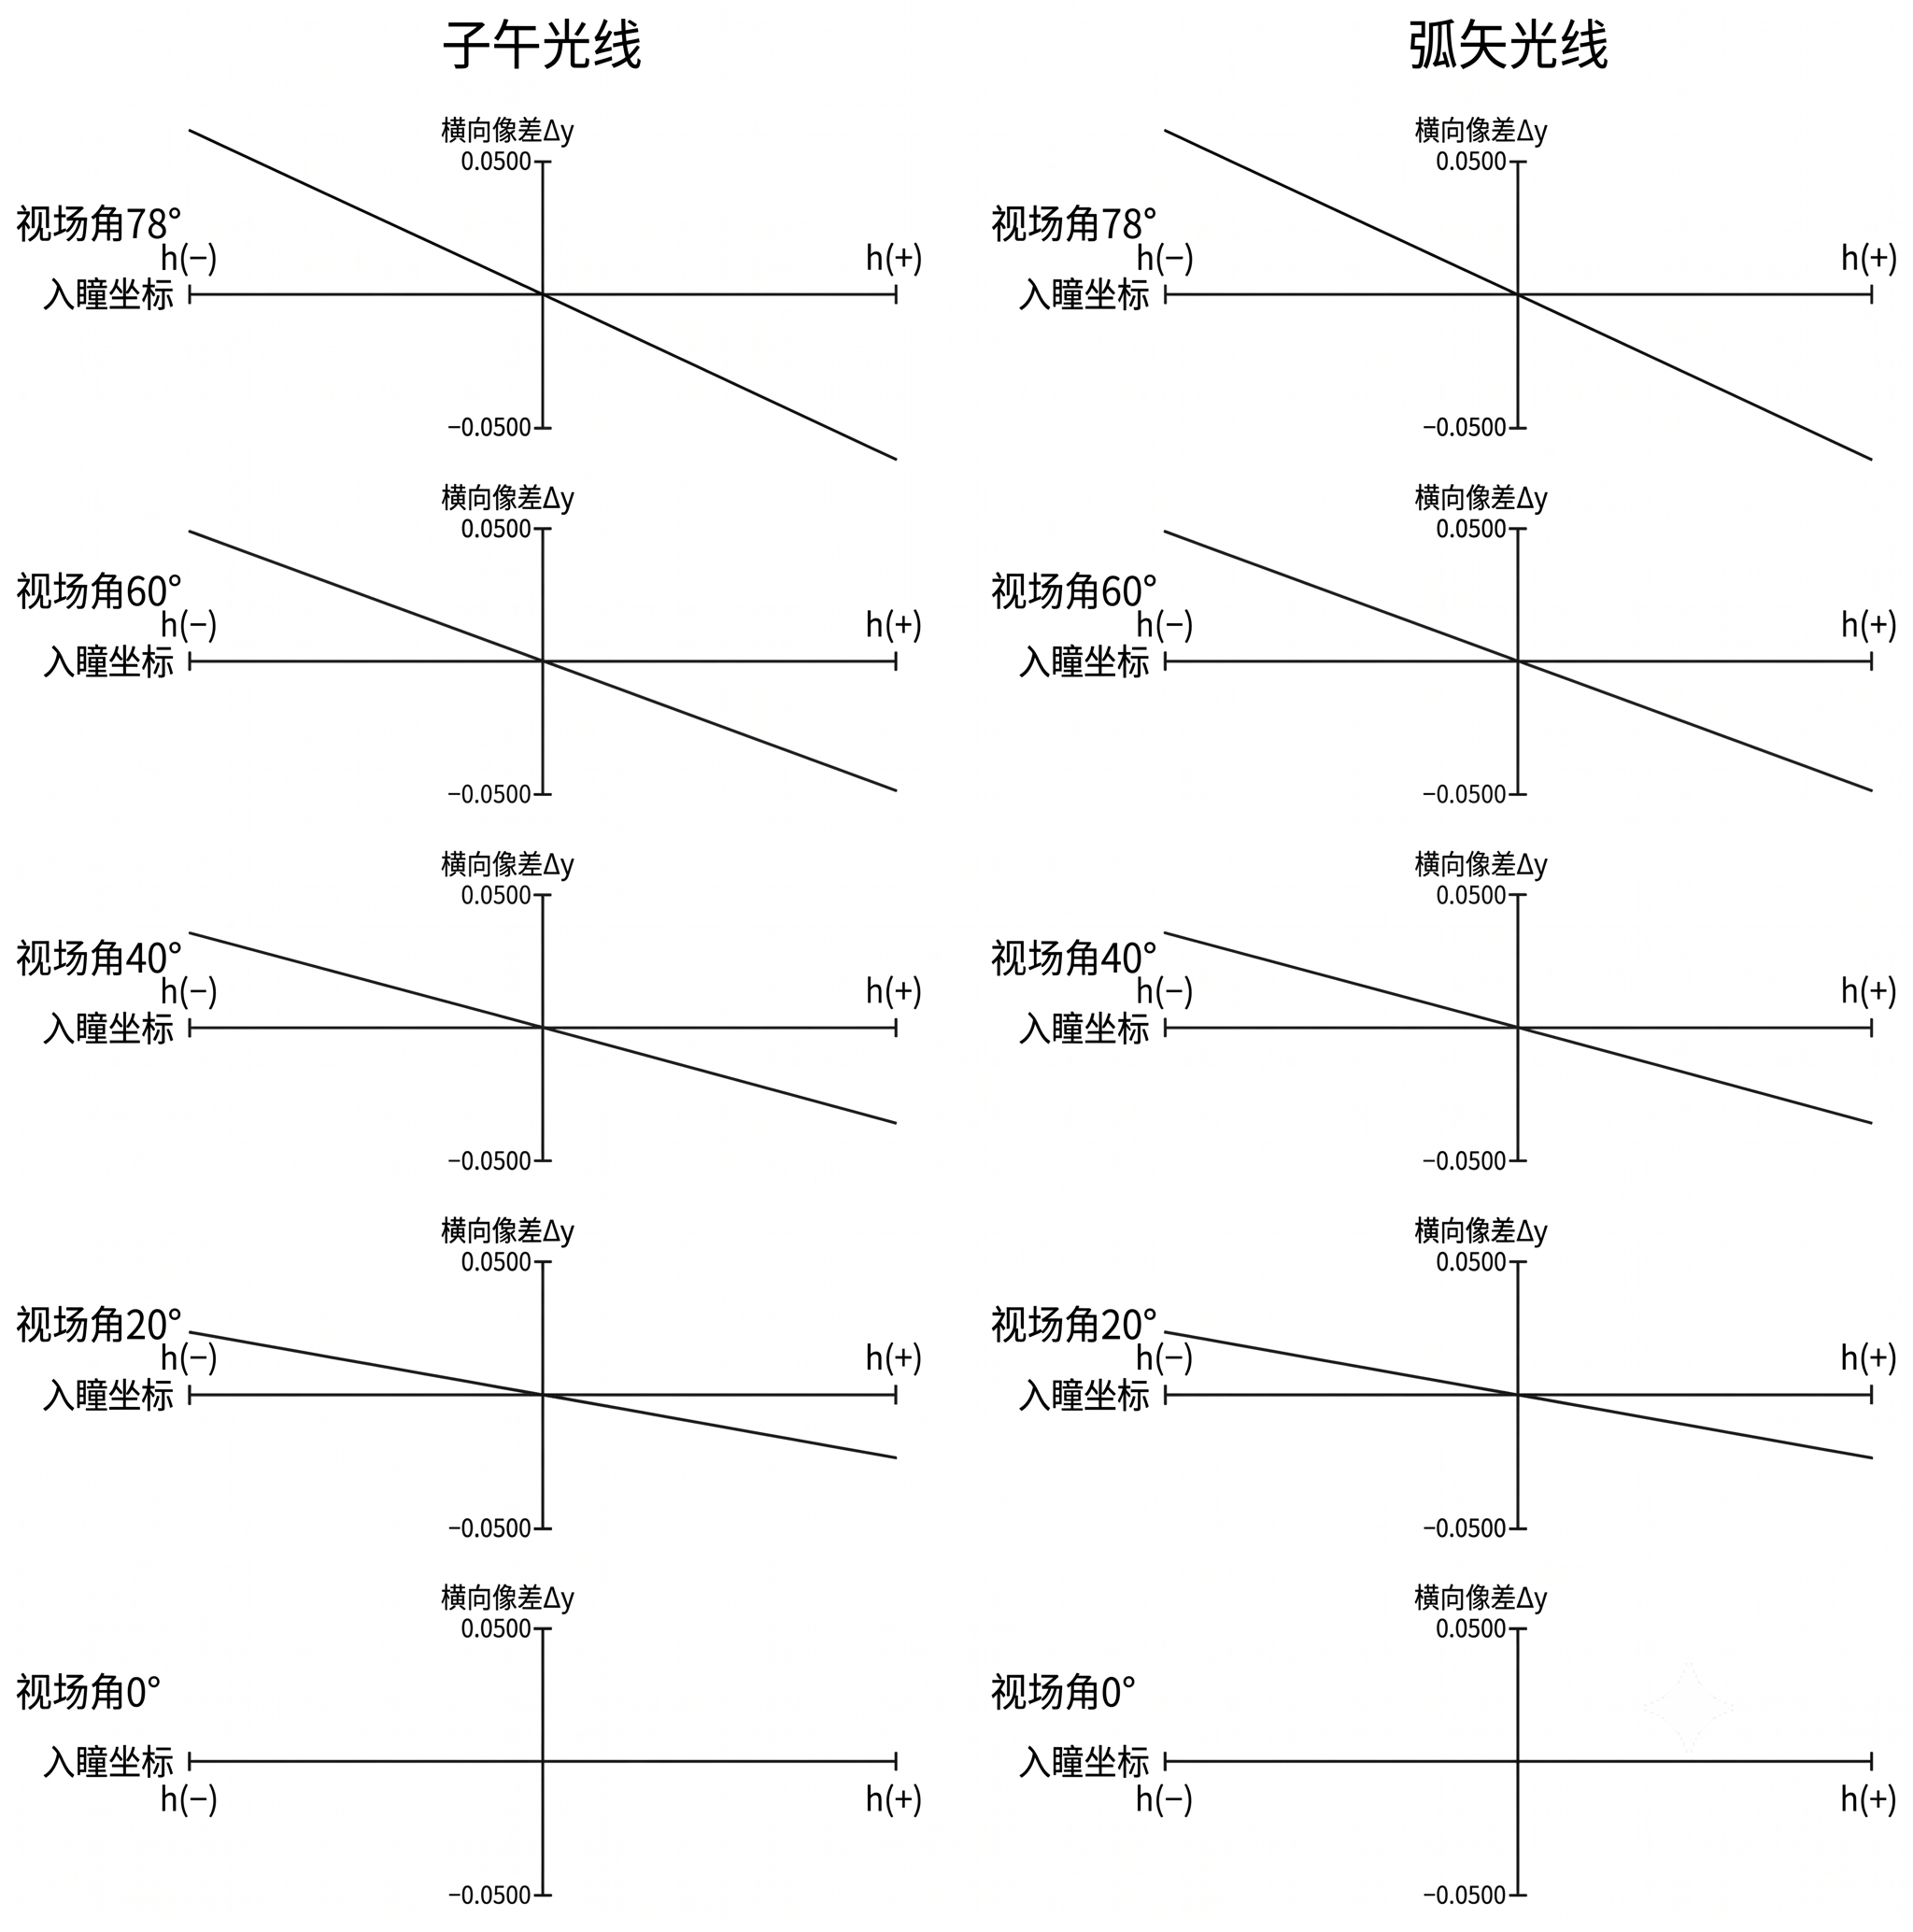
\includegraphics[width=.32\textwidth,height=.25\textheight,keepaspectratio]{Figure/图片21.png}\hfill
                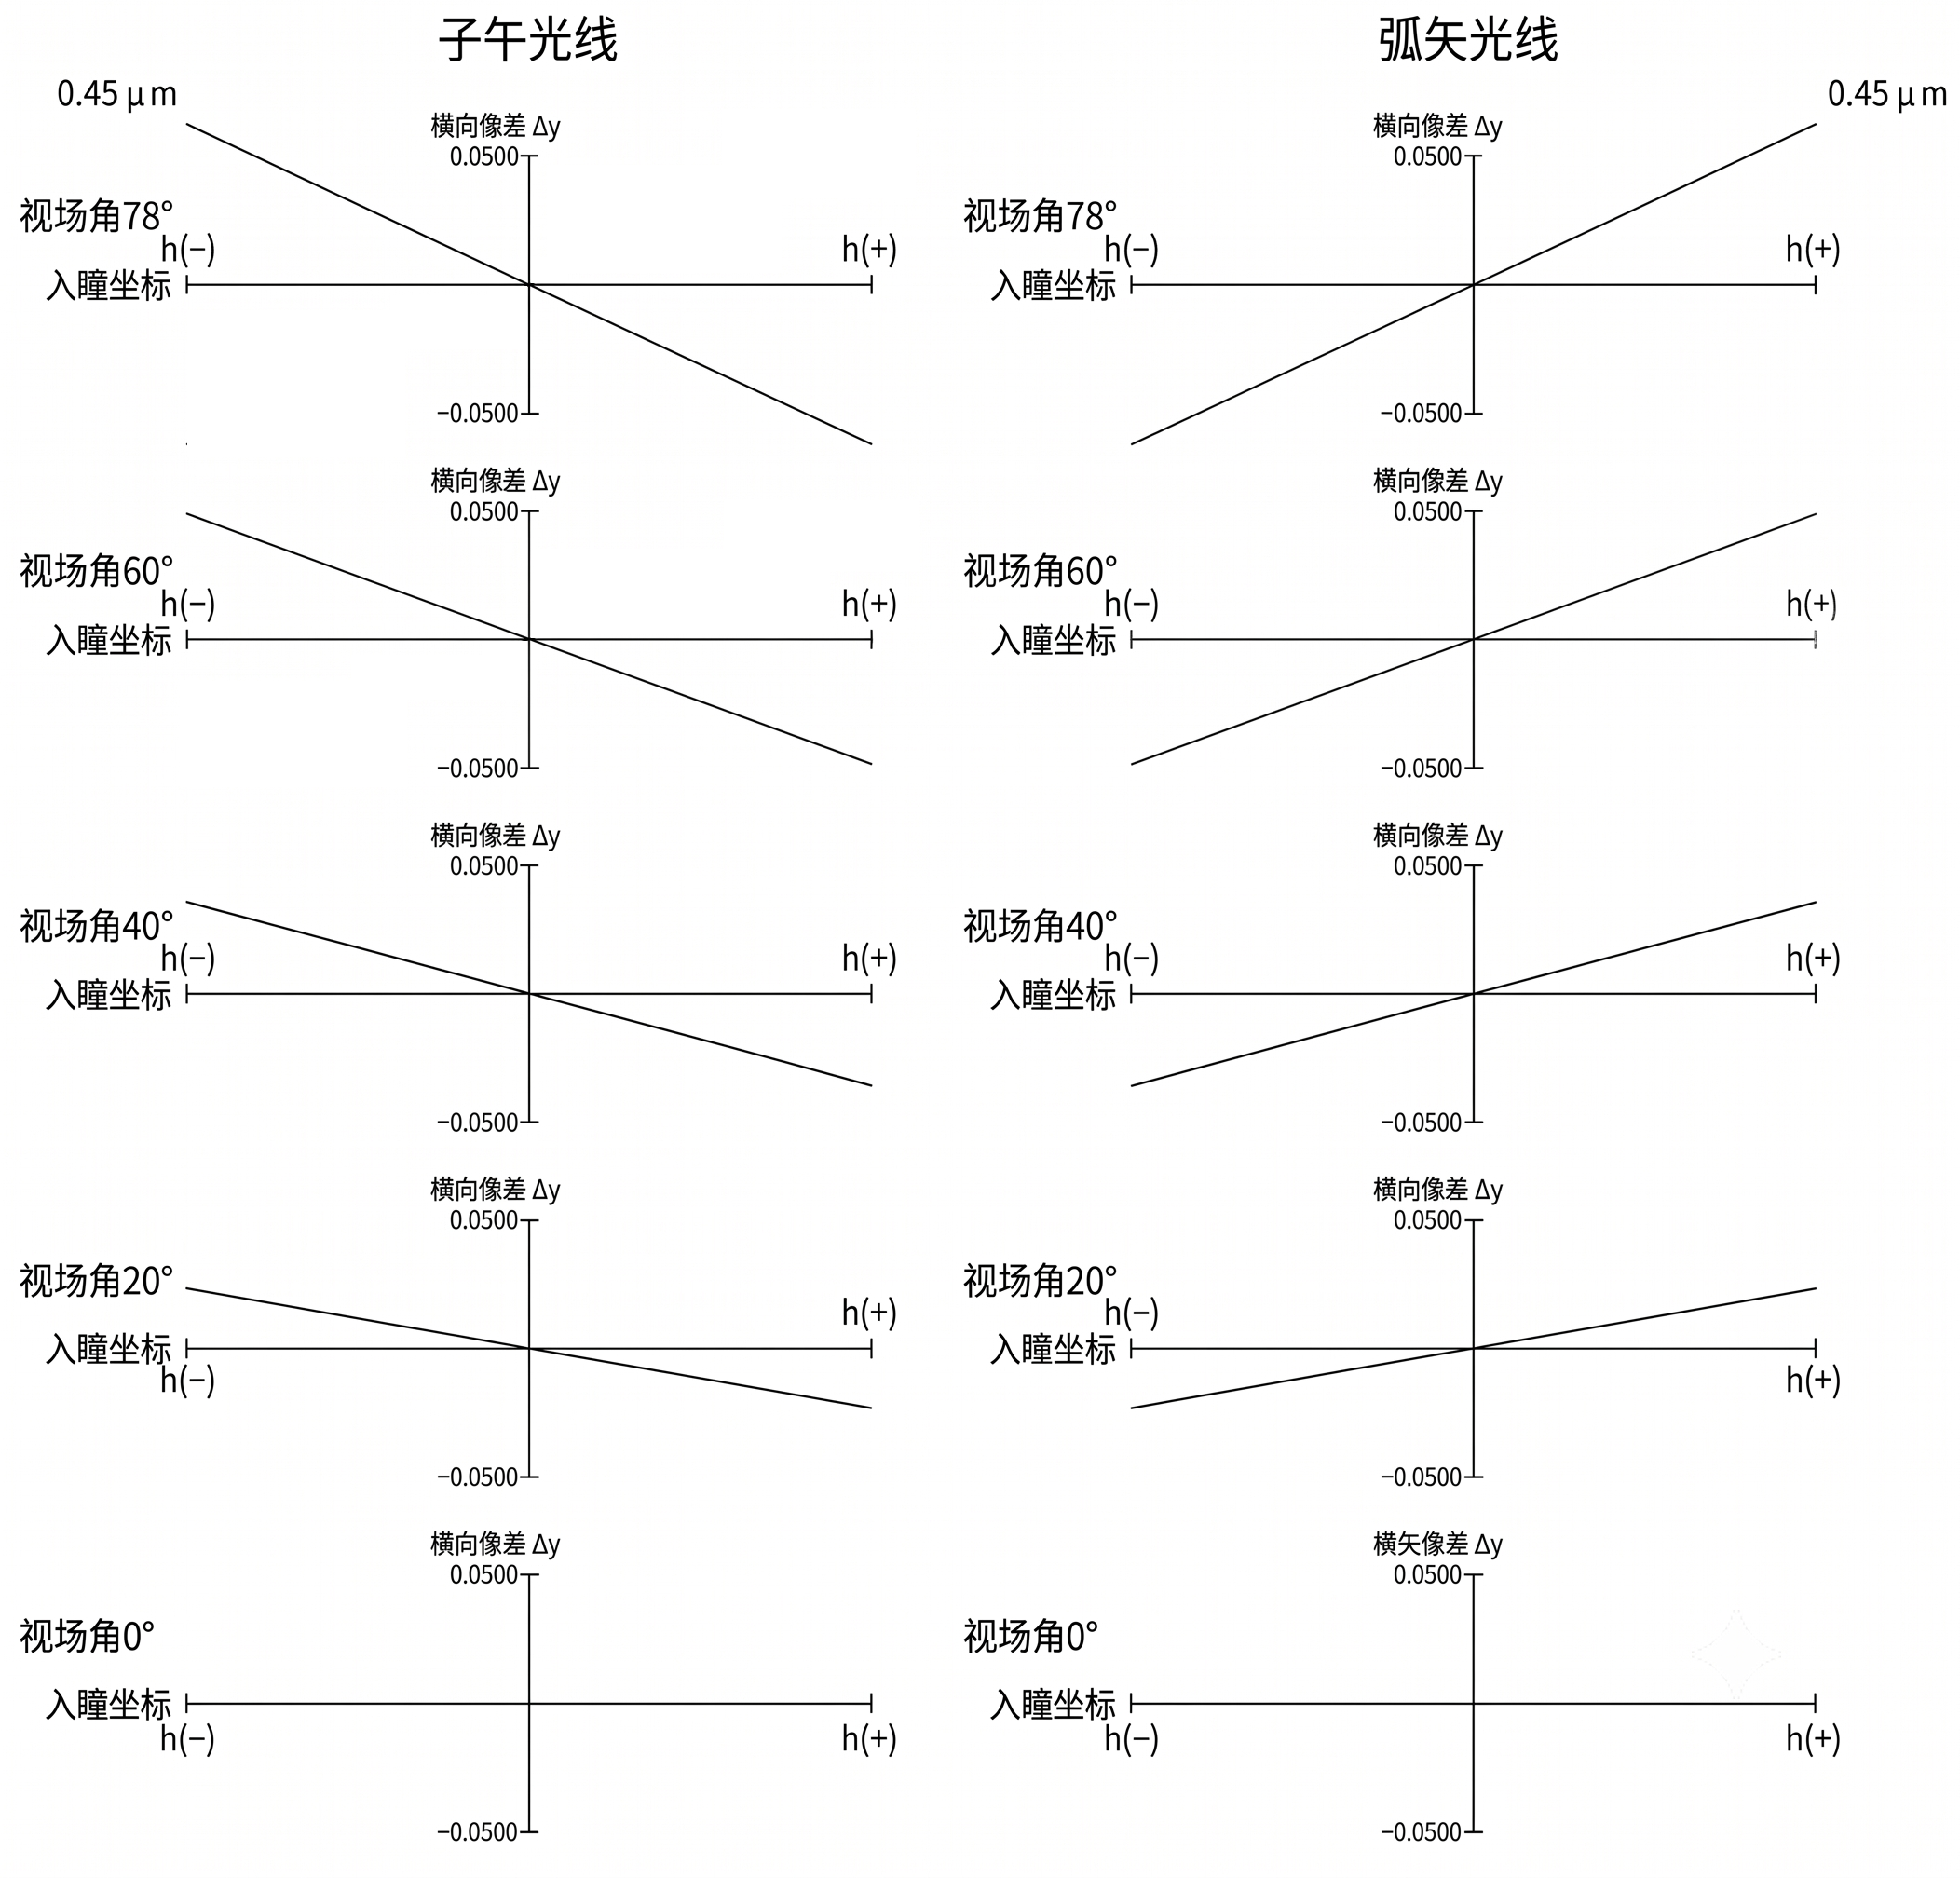
\includegraphics[width=.32\textwidth,height=.25\textheight,keepaspectratio]{Figure/图片22.png}
                \vspace{3pt}
                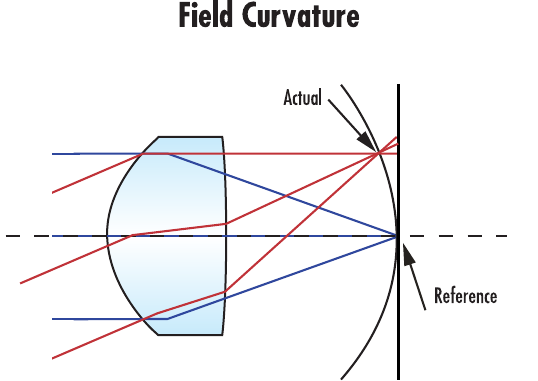
\includegraphics[width=\textwidth,height=.24\textheight,keepaspectratio]{Figure/Edmund/aberrations-4v2.png}
                \caption{上：离焦、场曲、像散的 Ray Fan；下：场曲的弯曲最佳像面}
                \label{fig:linear_field_curvature_main}
            \end{figure}
        \end{column}
        \hfill
        \begin{column}{.47\textwidth}
            \begin{block}{场曲}
                不同视场的最佳焦点落在不同轴向位置，本质上由 Petzval 和决定；移动平面探测器只能在中心和边缘之间折中。
            \end{block}

            \begin{block}{像散}
                子午与弧矢两组光线的最佳焦点分离，因此同一点物会先后形成两条正交焦线，中间只是最小弥散圆。
            \end{block}

            \begin{alertblock}{诊断顺序}
                先看不同视场的最佳焦点是否移动，再看 Tangential/Sagittal 两条曲线是否分离。
            \end{alertblock}
        \end{column}
    \end{columns}
\end{frame}

\englishtitle{Meridional and Sagittal Planes}
\begin{frame}{子午/弧矢：像散诊断所需的两个切面}
\label{1.12}
    \begin{columns}[T]
        \begin{column}{.56\textwidth}
            \begin{figure}
                \centering
                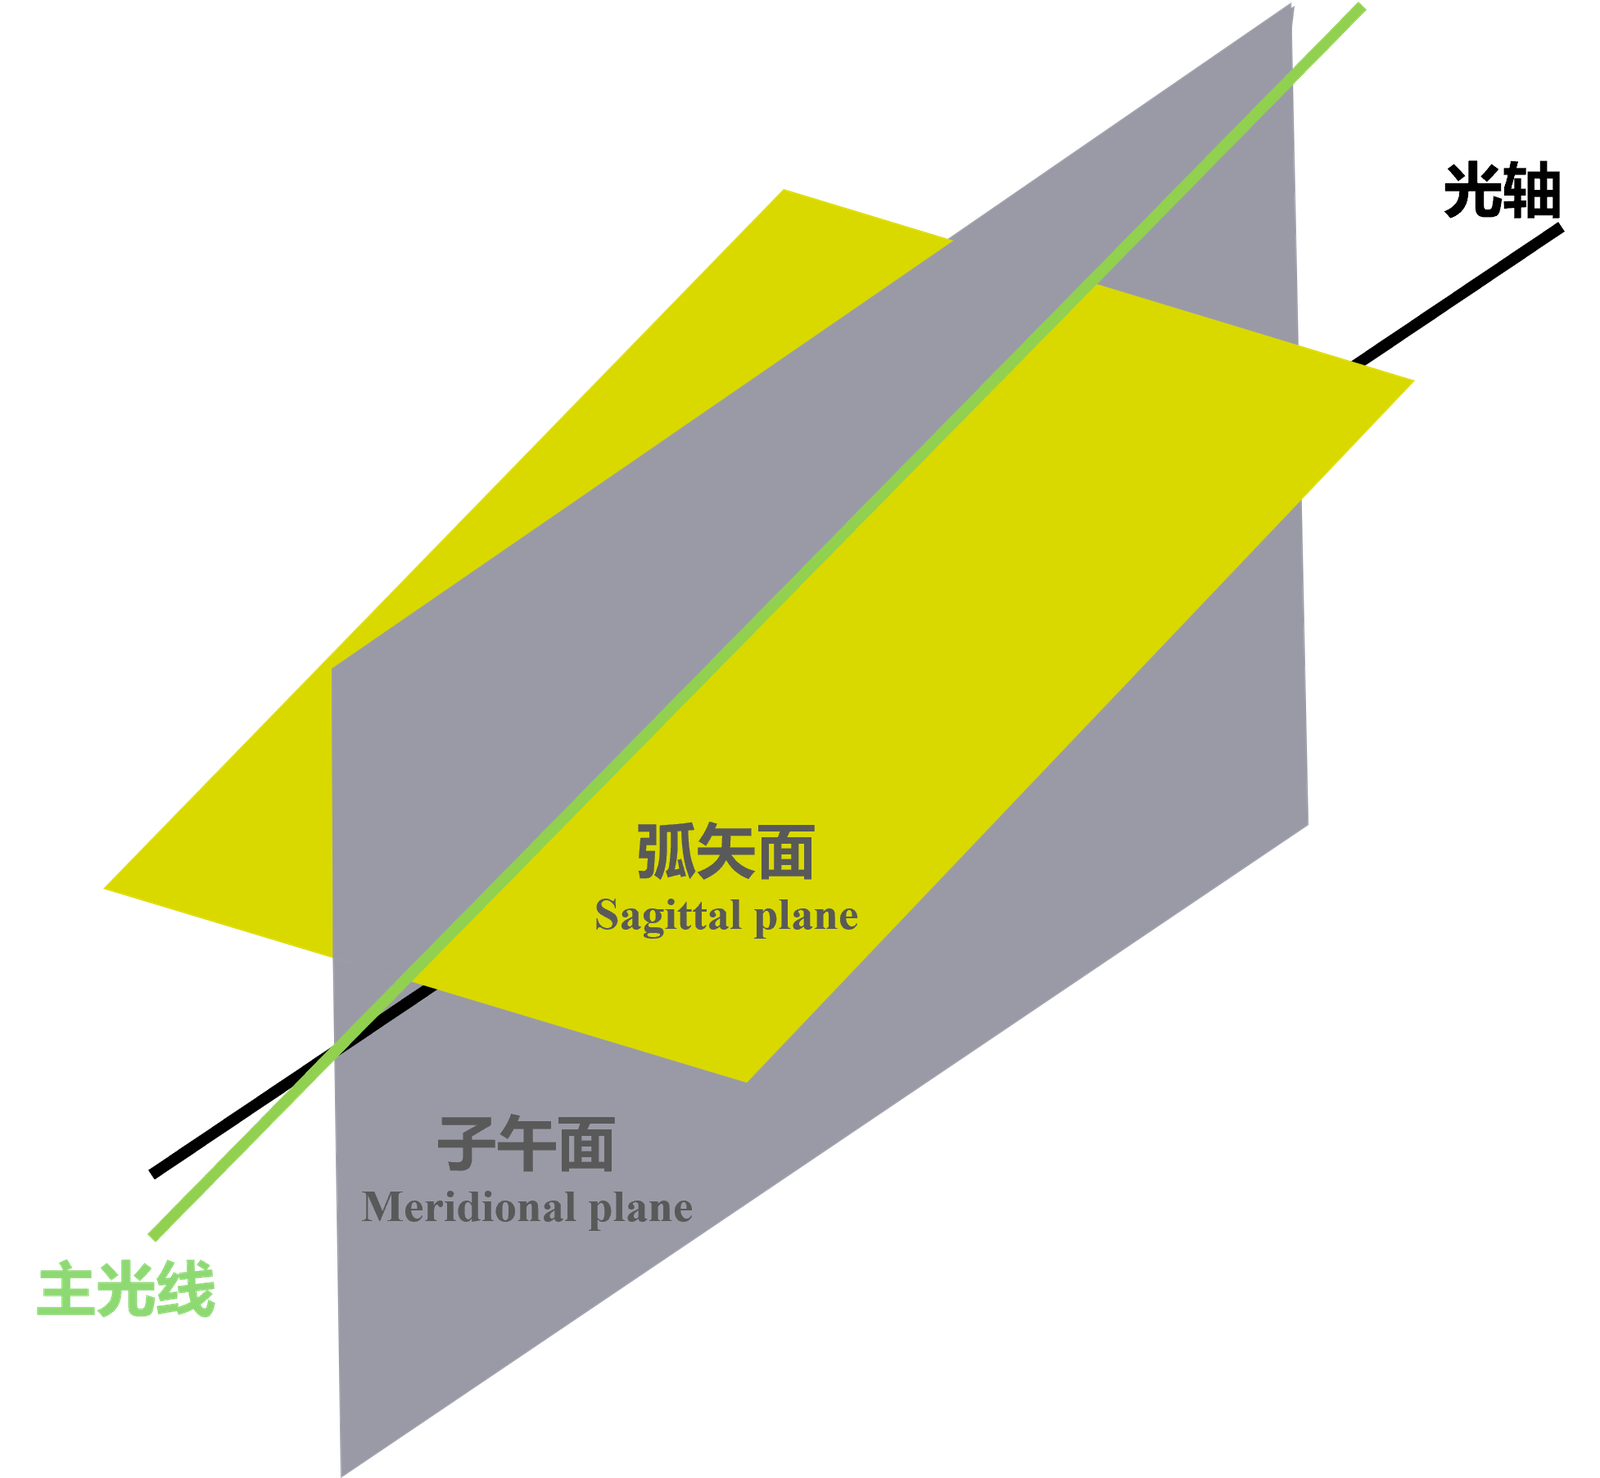
\includegraphics[width=.24\textwidth,height=.29\textheight,keepaspectratio]{Figure/图片18.png}\hfill
                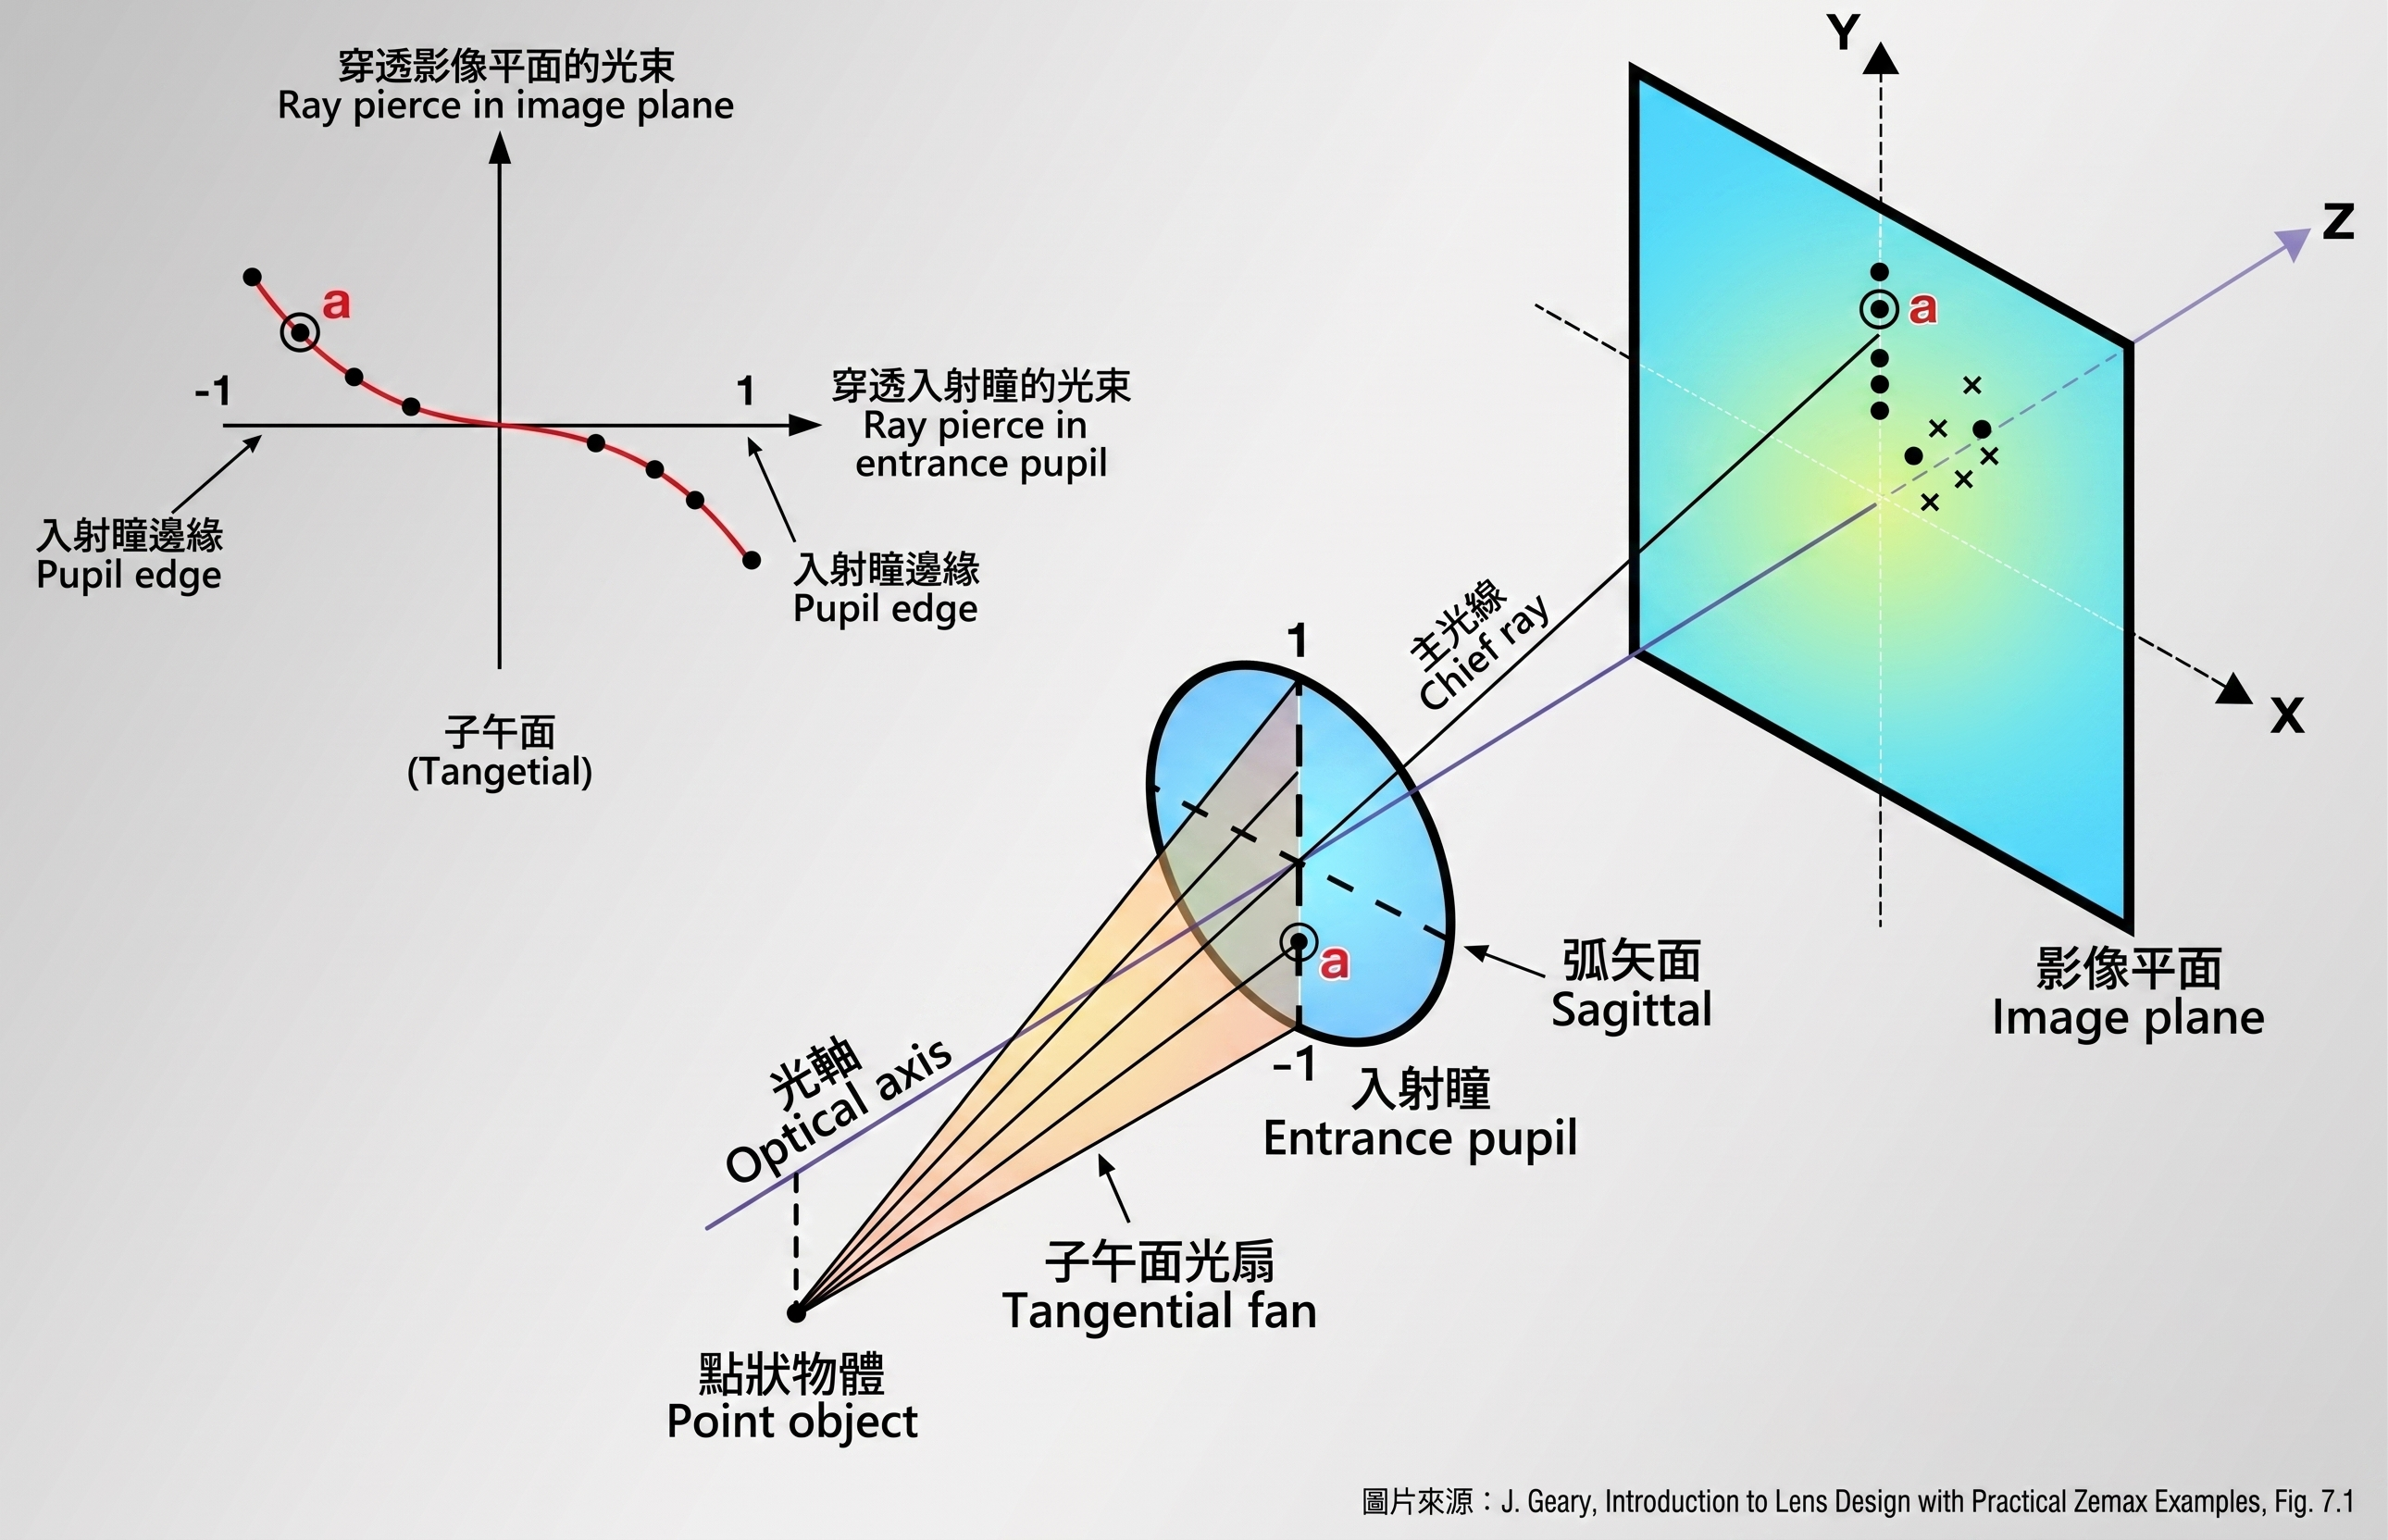
\includegraphics[width=.72\textwidth,height=.29\textheight,keepaspectratio]{Figure/图片26.png}
                \vspace{3pt}
                
\includegraphics[width=.46\textwidth,height=.18\textheight,keepaspectratio]{Figure/Edmund/abberations-2a.png}\hfill
                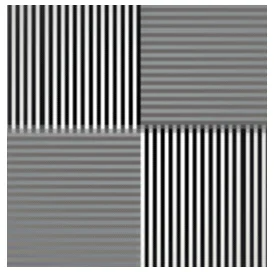
\includegraphics[width=.46\textwidth,height=.18\textheight,keepaspectratio]{Figure/Edmund/abberations-2b.png}
                \caption{上：子午面与弧矢面；下：像散导致两个方向不能同时清晰}
                \label{fig:meridional_sagittal_astigmatism_main}
            \end{figure}
        \end{column}
        \hfill
        \begin{column}{.44\textwidth}
            \begin{itemize}
                \item \textbf{子午面}包含光轴和主光线。
                \item \textbf{弧矢面}与子午面正交，并同样经过主光线。
                \item Zemax 的 Tangential Fan / Sagittal Fan，就是分别在这两个切面里观察 Ray Fan。
                \item 若只靠整体移动像面，通常只能在两条焦线之间折中，不能真正消掉像散。
            \end{itemize}

            \begin{block}{工程处理}
                常见手段包括弯月透镜、对称结构、调整光阑位置或降低离轴会聚角。
            \end{block}
        \end{column}
    \end{columns}
\end{frame}

\subsection{色散、阿贝图与玻璃选择}
\label{sec:1.5}

\englishtitle{Abbe Diagram and Chromatic Correction}
\begin{frame}{阿贝图：把色差问题落到材料选择}
\label{1.13}
    \begin{columns}[T]
        \begin{column}{.45\textwidth}
            \begin{figure}
                \centering
                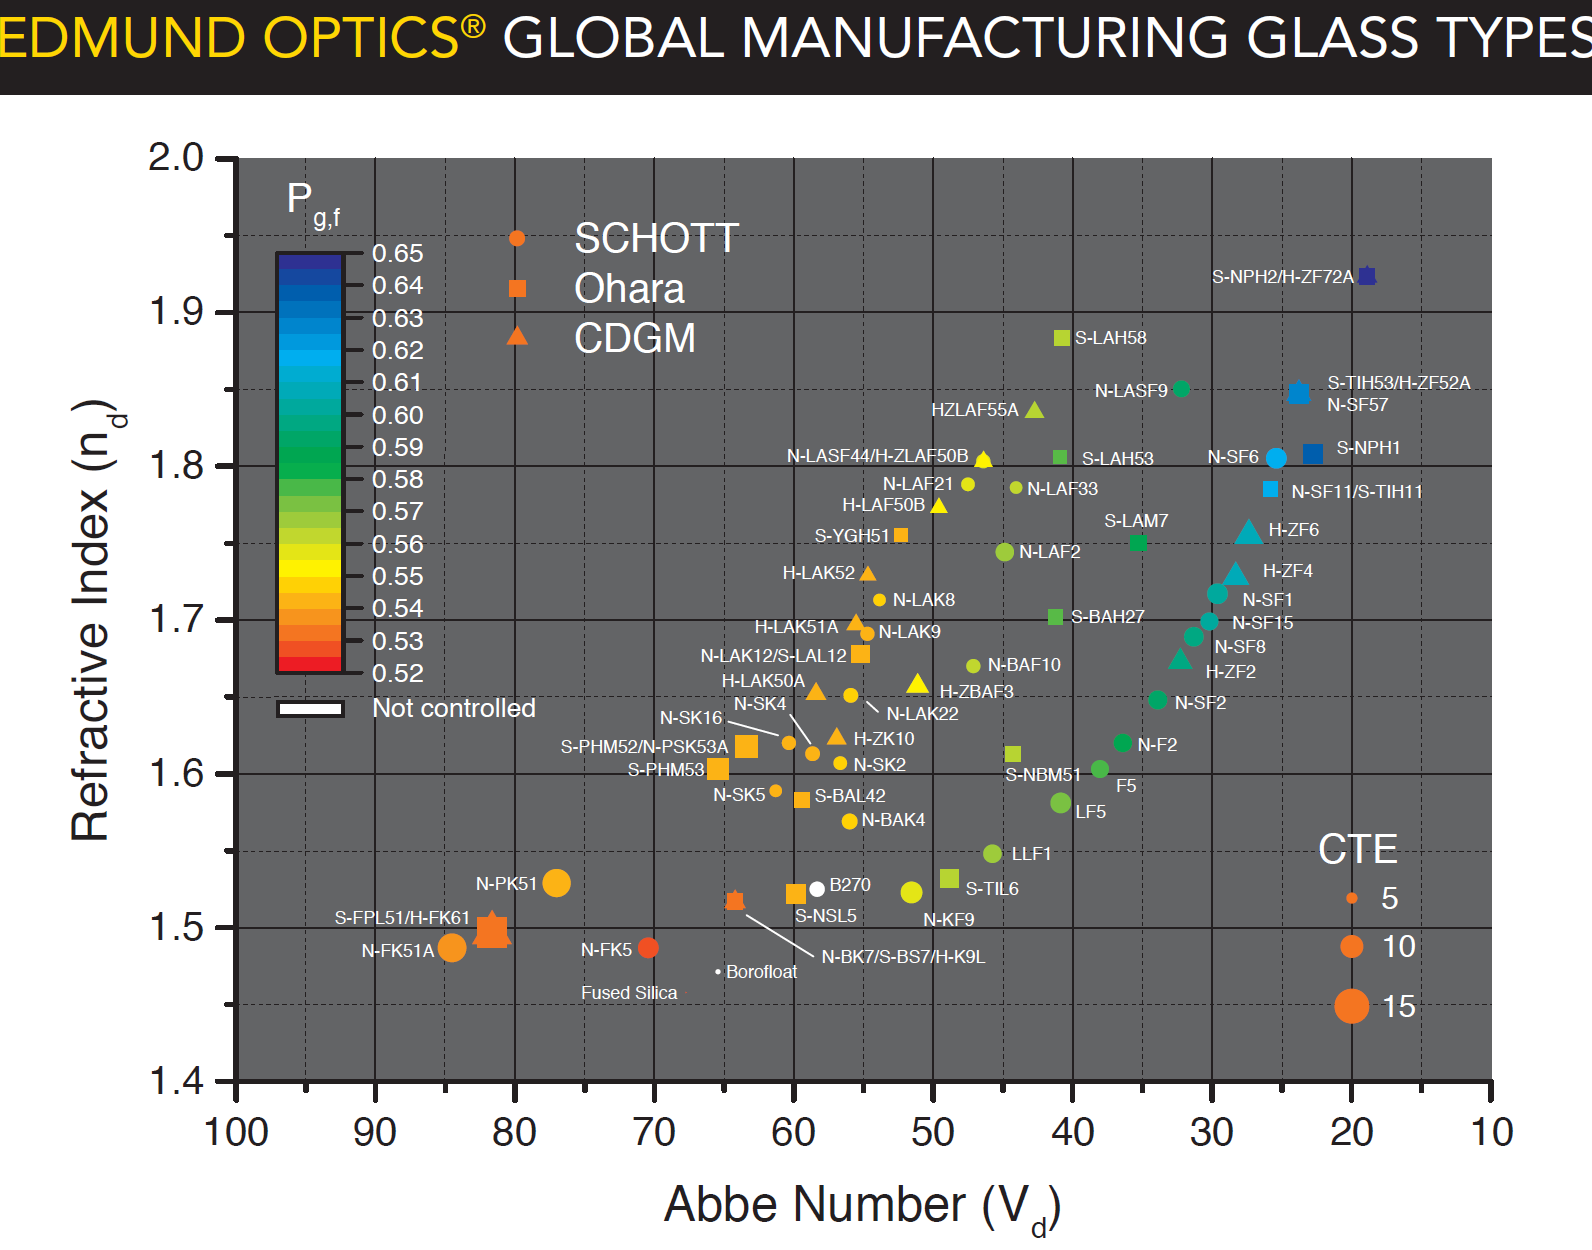
\includegraphics[width=.98\textwidth,height=.45\textheight,keepaspectratio]{Figure/Abbe.png}
                \caption{阿贝图：折射率与色散能力的材料地图}
                \label{fig:abbe_main}
            \end{figure}
        \end{column}
        \hfill
        \begin{column}{.55\textwidth}
            \textbf{色散是材料属性：}
            \begin{equation}
                \nu_d = \frac{n_d-1}{n_F-n_C}
                \label{eq:abbe_main}
            \end{equation}

            \begin{itemize}
                \item 低色散冕牌玻璃和高色散火石玻璃组合，是消色差双胶合的基本思路。
                \item Achromat 通常先让两种代表波长共焦；Apochromat 进一步压低第三波长和二级光谱残差。
                \item 对显微物镜，色差校正等级会直接推高材料自由度、镜片数量和制造成本。
            \end{itemize}

            \begin{alertblock}{合并后的主线}
                色差不要和材料选择分开讲：先看阿贝图决定材料空间，再回到 Ray Fan/OPD 判断色差是否真的被压低。
            \end{alertblock}
        \end{column}
    \end{columns}
\end{frame}

\englishtitle{Chromatic Aberration in Ray Fan}
\begin{frame}{色差在 Ray Fan 上怎么看}
\label{1.14}
    \begin{columns}[T]
        \begin{column}{.50\textwidth}
            \begin{figure}
                \centering
                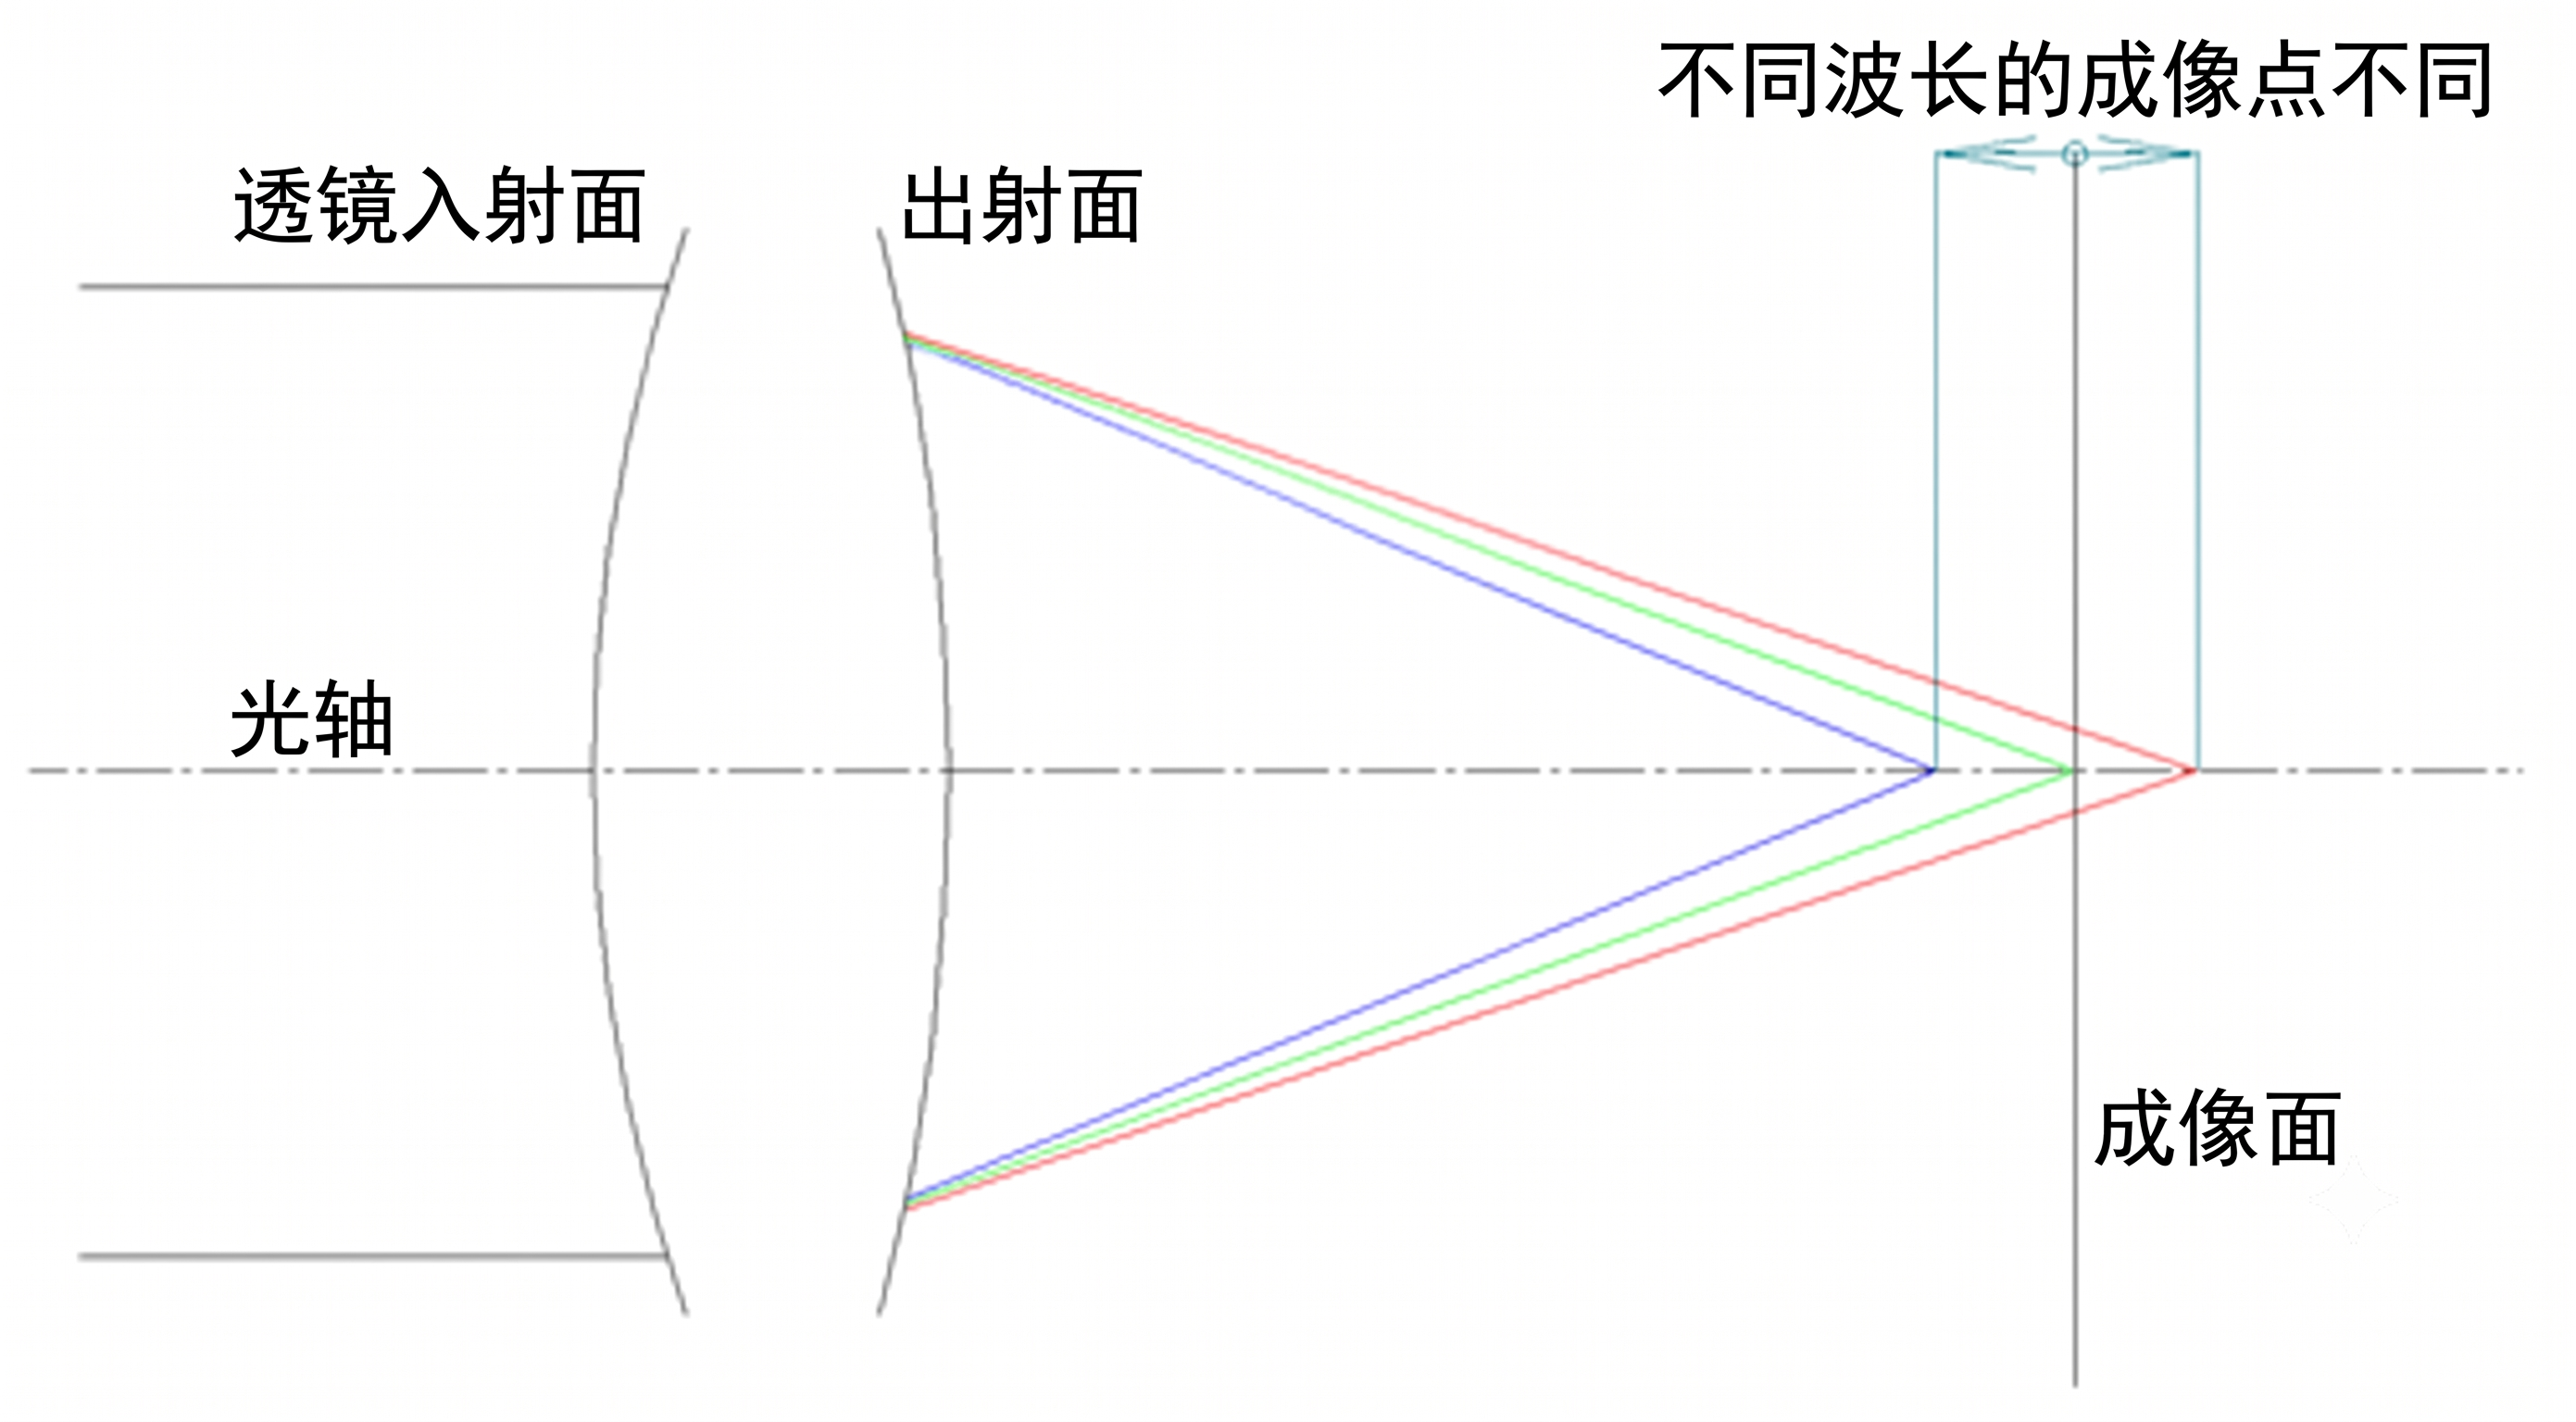
\includegraphics[width=.98\textwidth,height=.27\textheight,keepaspectratio]{Figure/图片30.png}
                \vspace{2pt}
                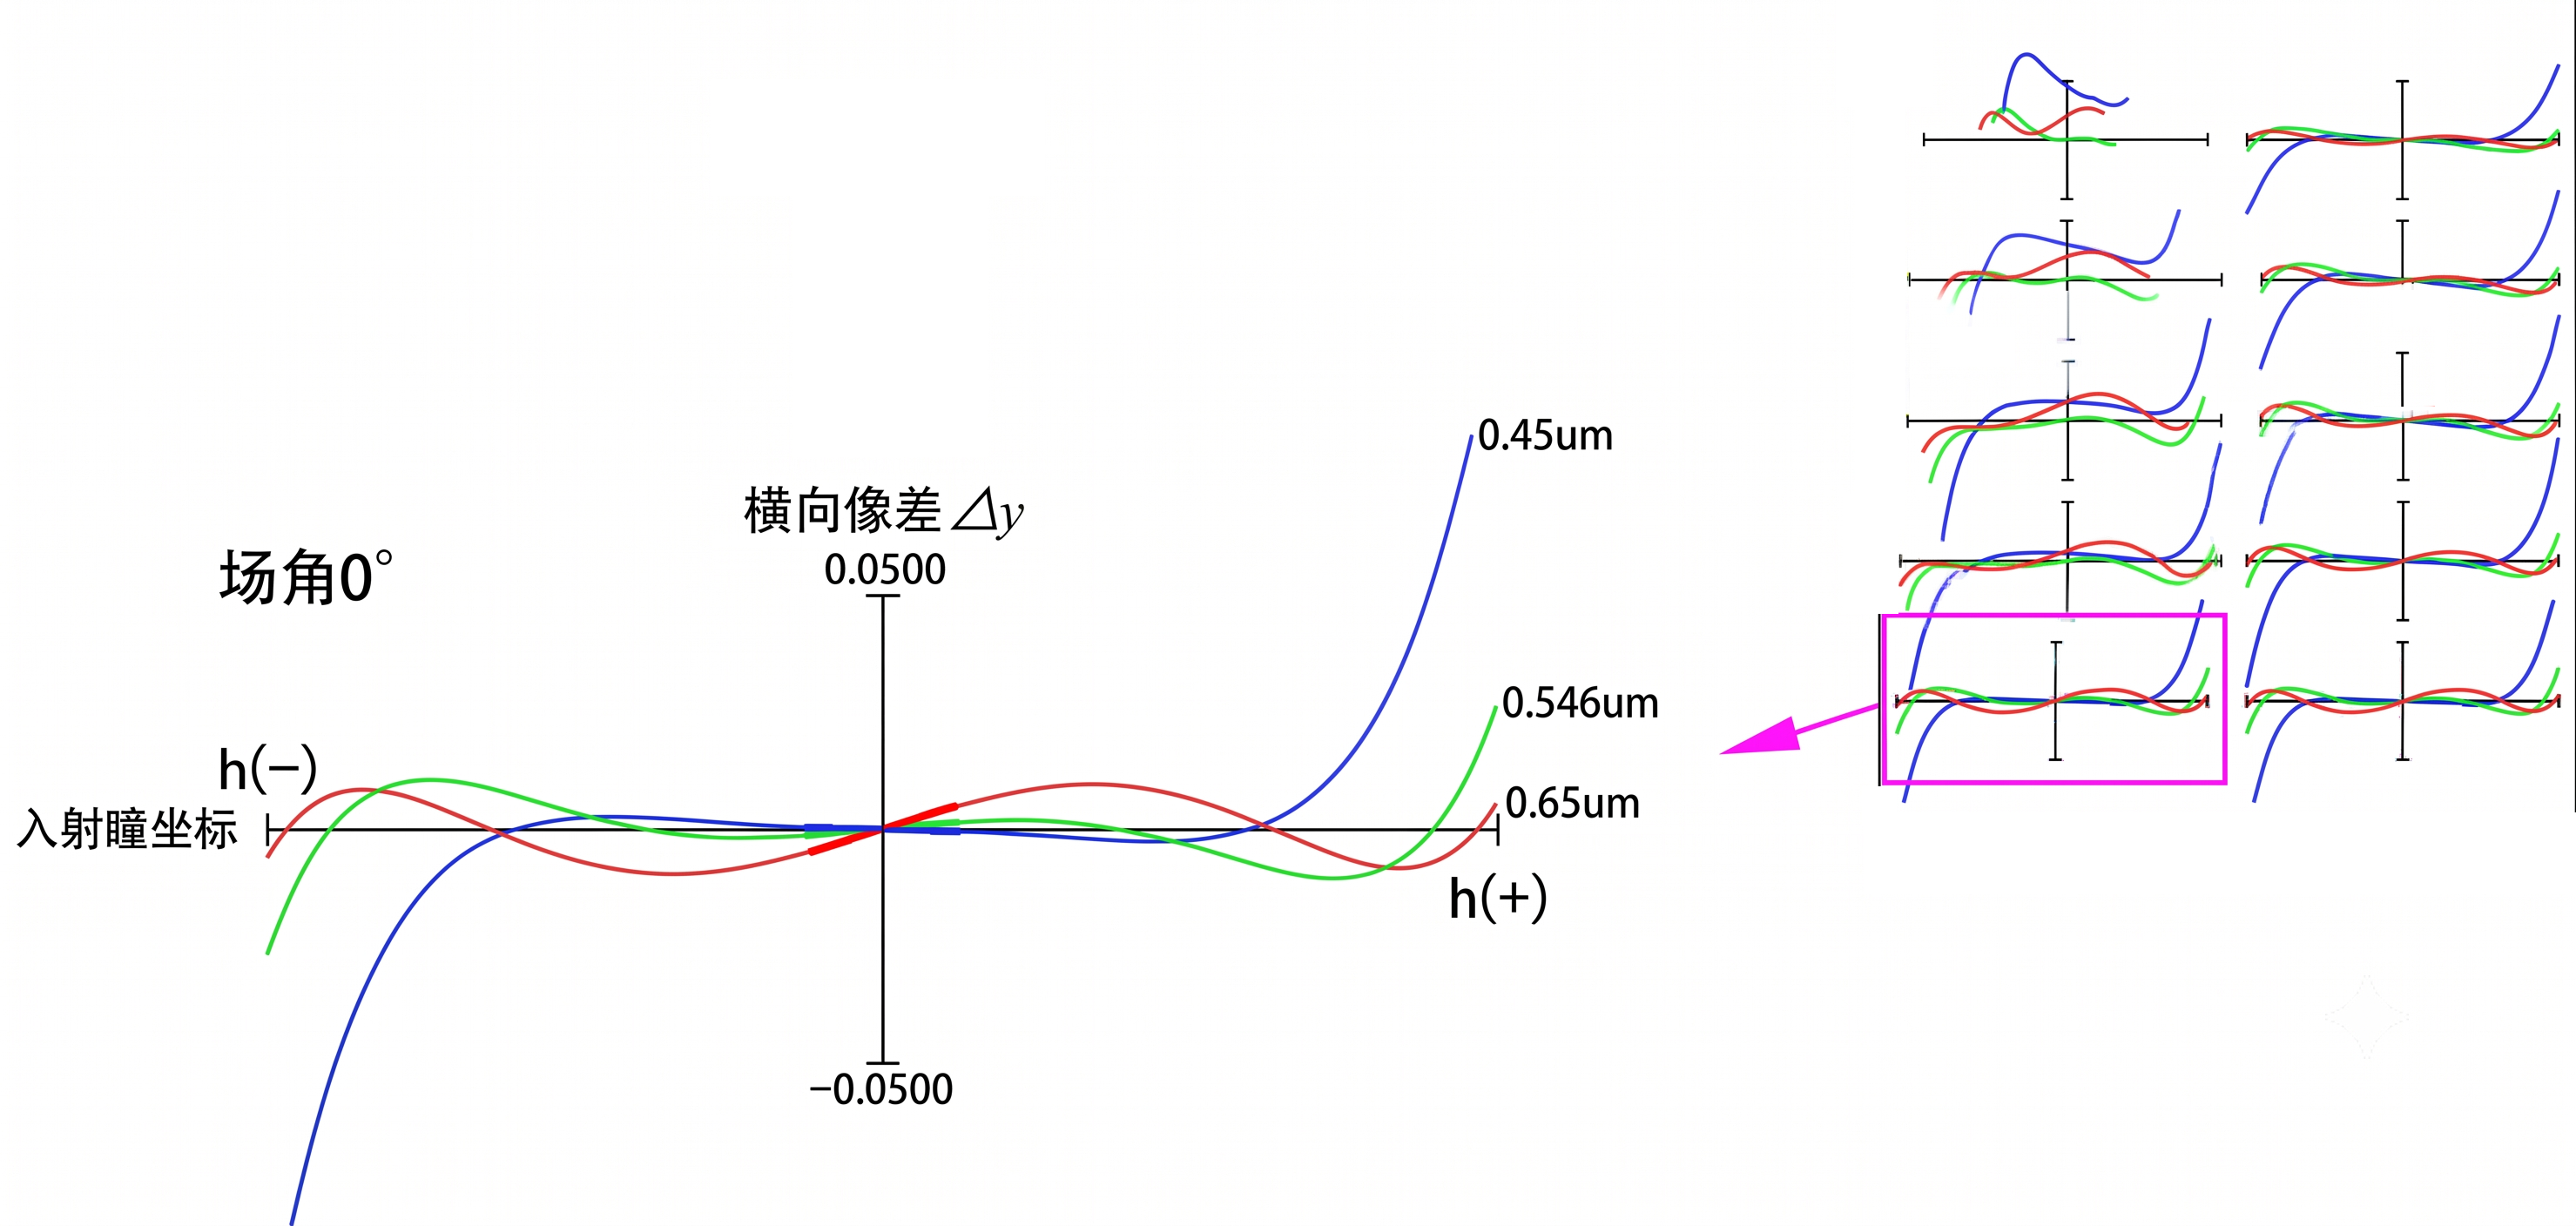
\includegraphics[width=.98\textwidth,height=.19\textheight,keepaspectratio]{Figure/图片28.png}
                \caption{轴向色差：不同波长近轴焦点位置不同}
                \label{fig:axial_color_main}
            \end{figure}
        \end{column}
        \hfill
        \begin{column}{.50\textwidth}
            \begin{figure}
                \centering
                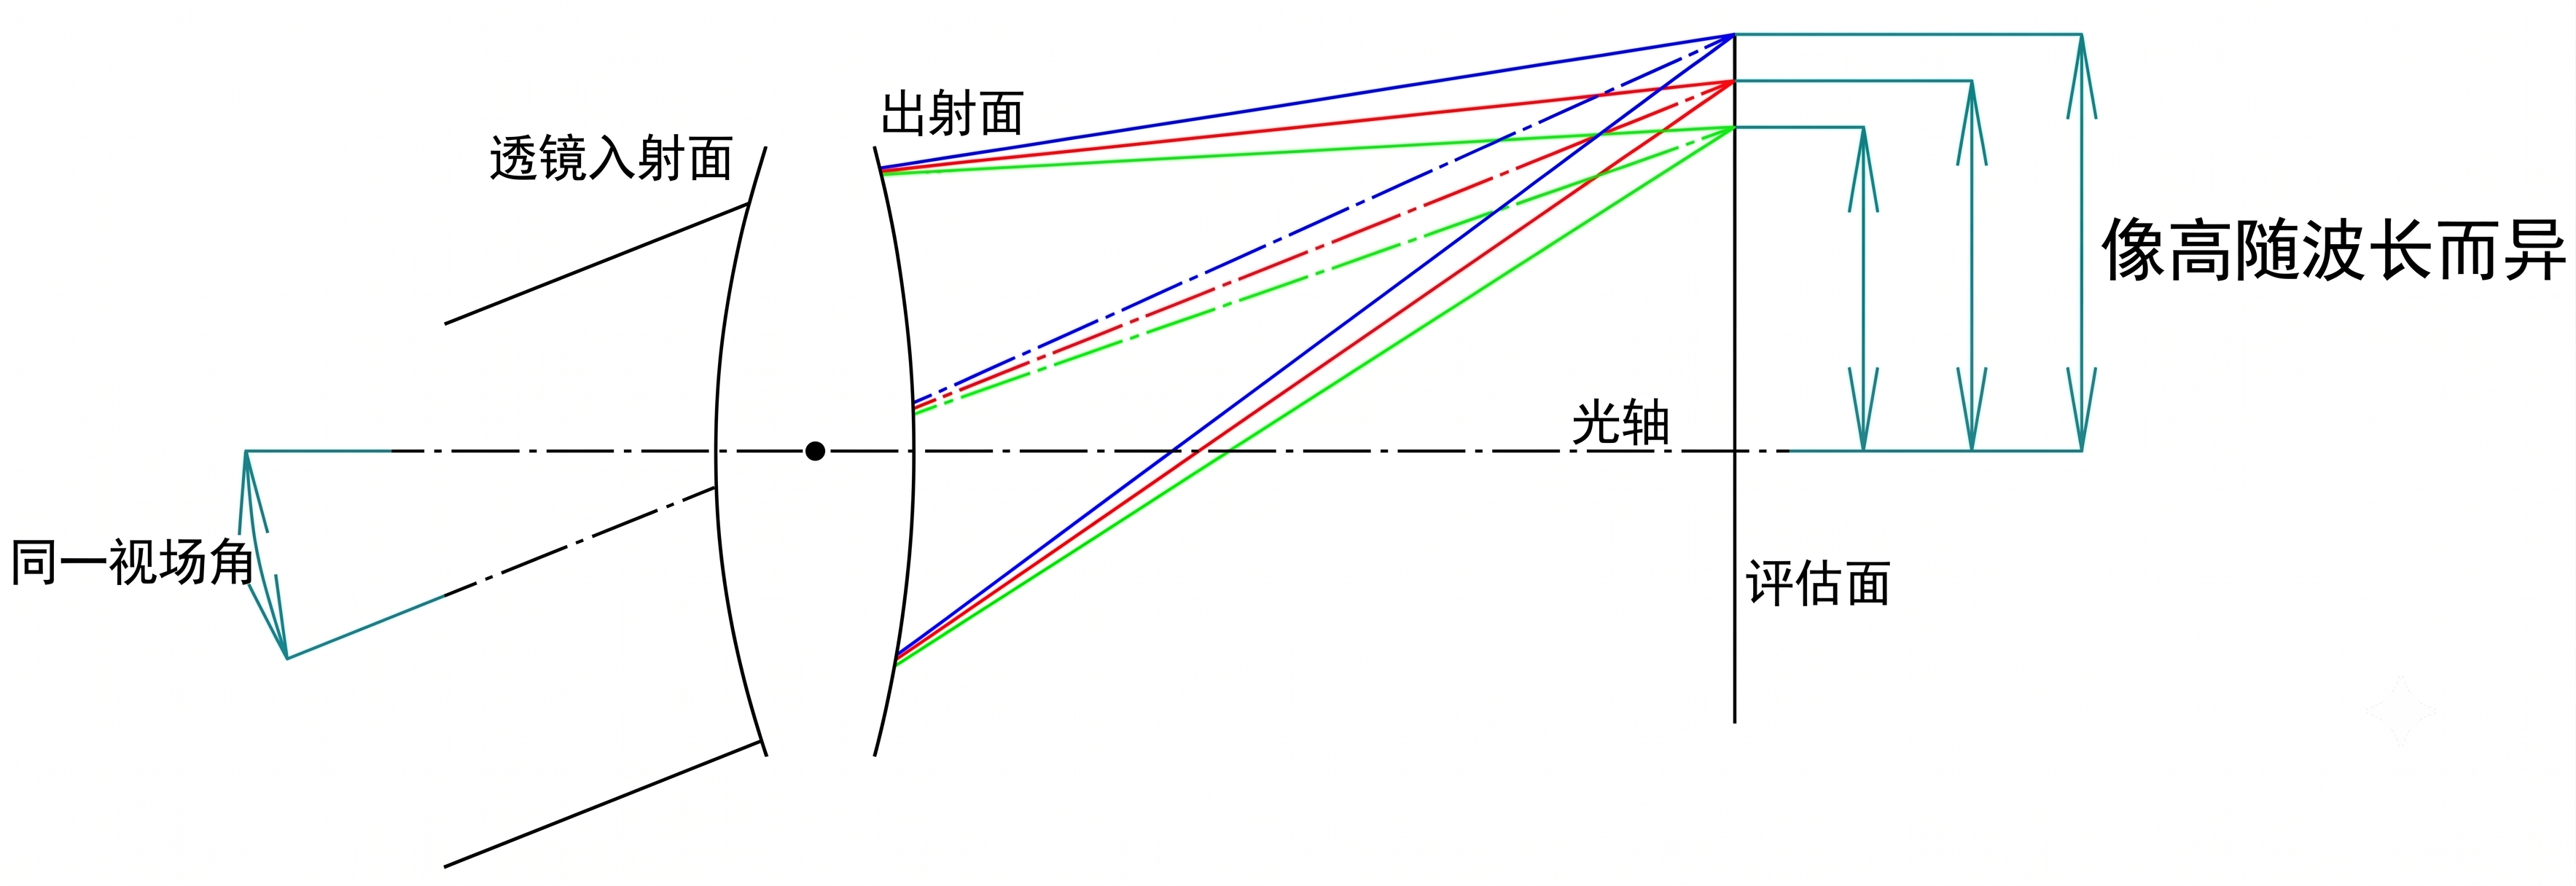
\includegraphics[width=.98\textwidth,height=.27\textheight,keepaspectratio]{Figure/图片31.png}
                \vspace{2pt}
                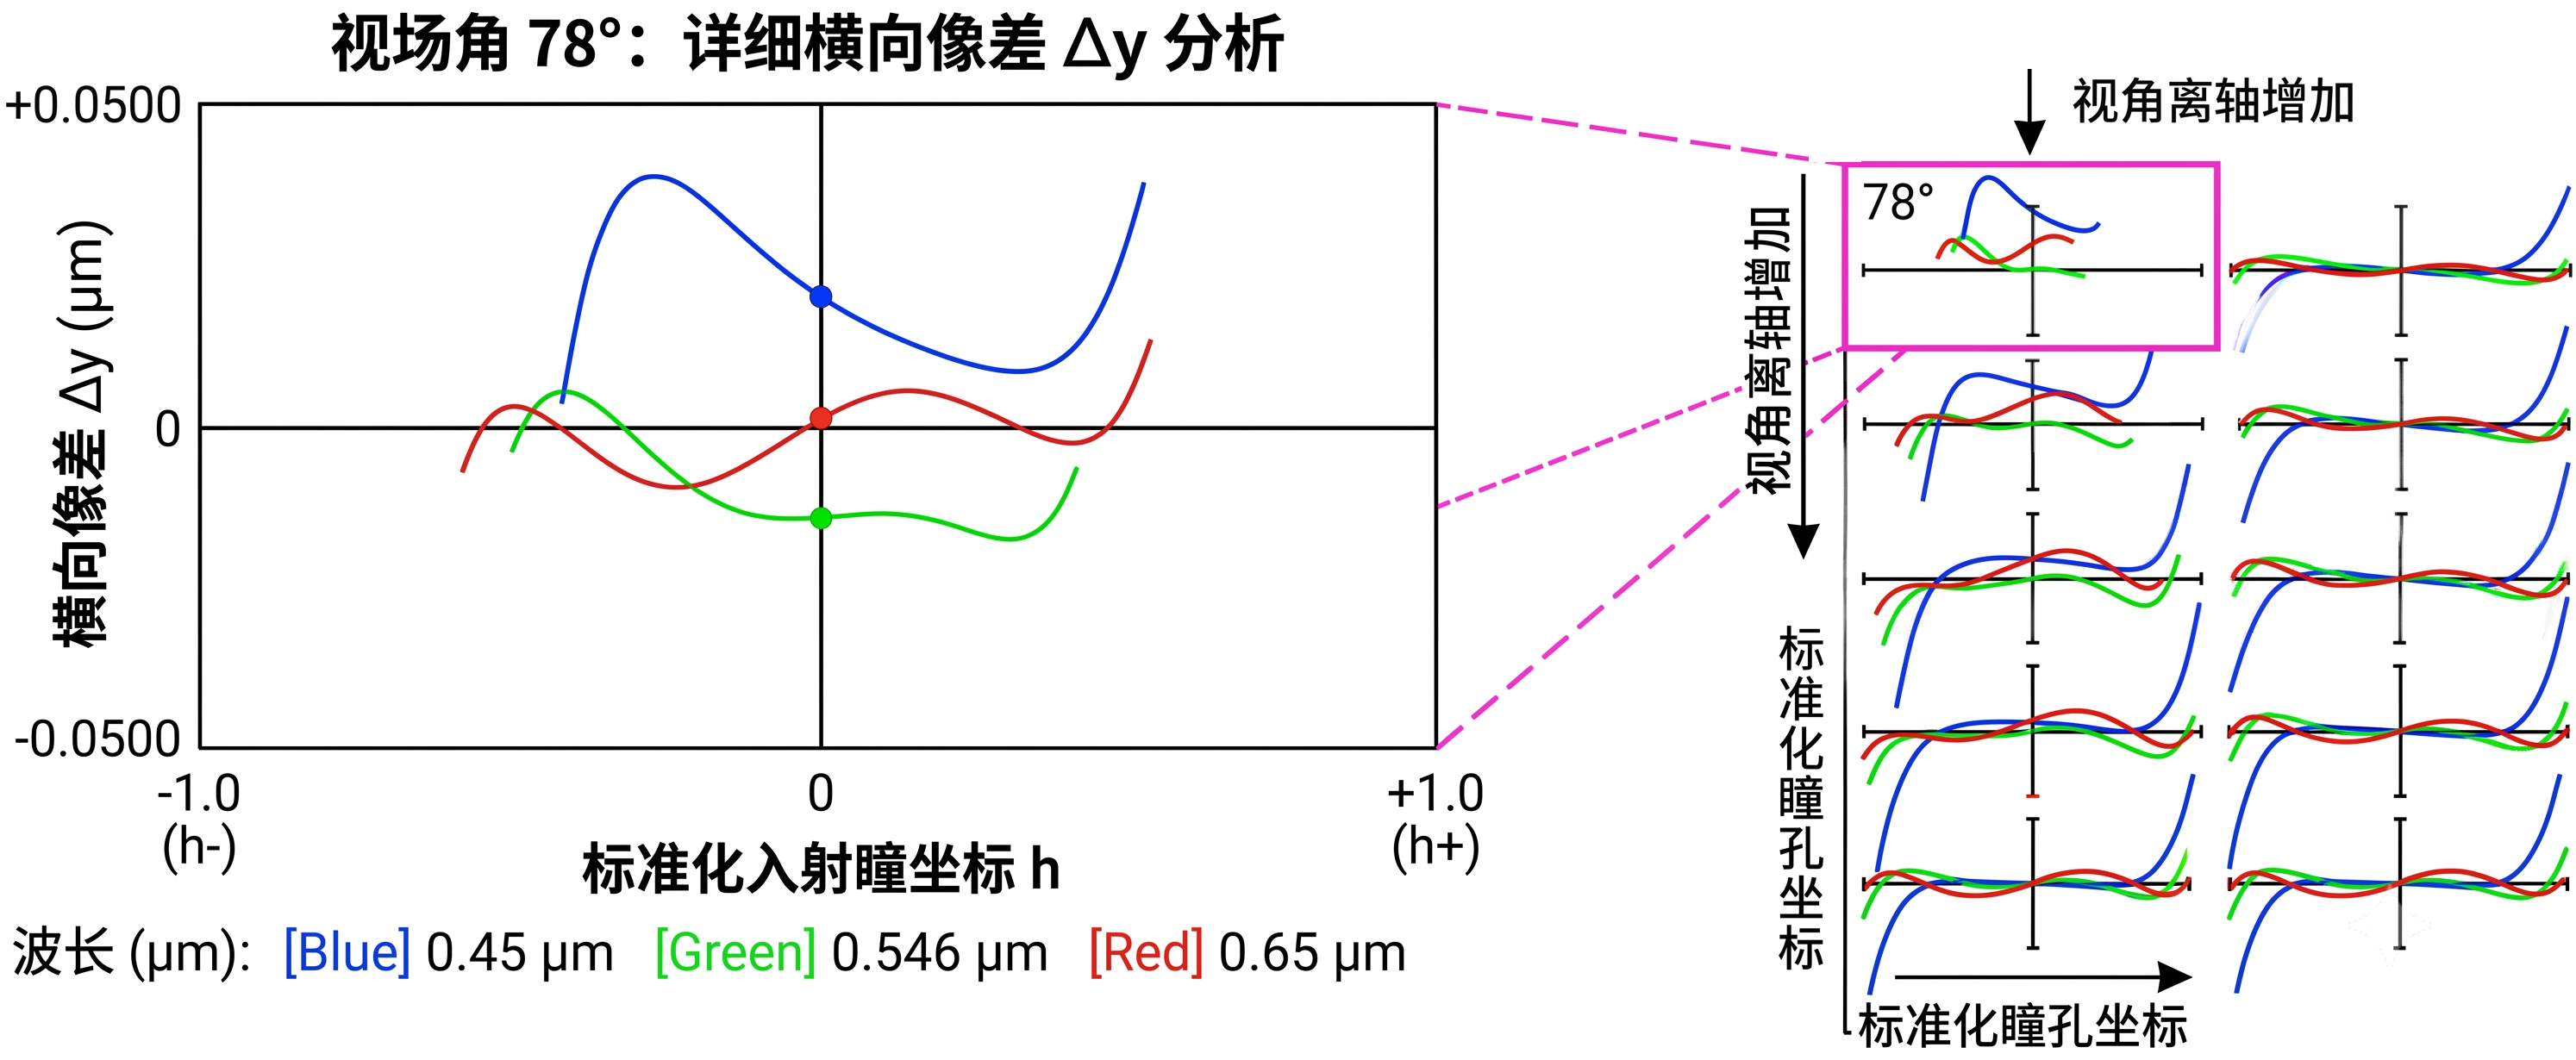
\includegraphics[width=.98\textwidth,height=.19\textheight,keepaspectratio]{Figure/图片29.png}
                \caption{倍率色差：不同波长主光线像高不同}
                \label{fig:lateral_color_main}
            \end{figure}
        \end{column}
    \end{columns}

    \vspace{-4pt}
    \begin{table}
        \centering
        \scriptsize
        \renewcommand{\arraystretch}{1.25}
        \begin{tabular}{p{2.0cm}|p{4.2cm}|p{4.2cm}}
            \toprule
            \textbf{类型} & \textbf{Ray Fan 特征} & \textbf{优化抓手} \\
            \midrule
            轴向色差 & 同一视场下，不同波长在原点附近斜率不同 & 玻璃组合、多波长权重、消色差约束 \\
            倍率色差 & 轴外视场中，不同波长主光线截距不同 & 对称结构、主光线色散控制、离轴波长权重 \\
            \bottomrule
        \end{tabular}
    \end{table}
\end{frame}

\englishtitle{Glass Substitution Workflow}
\begin{frame}{玻璃替换：直接在真实玻璃目录中优化}
\label{1.15}
    \begin{columns}[T]
        \begin{column}{.45\textwidth}
            \begin{enumerate}
                \item 在 LDE 中将玻璃 Solve 类型设为 \alert{Substitute}。
                \item 选择供应商目录，如 Schott、Hoya、Ohara、CDGM。
                \item 构建 RMS Wavefront 或 MTF/Spot 相关评价函数。
                \item 使用 Hammer 或 Global Search 处理离散玻璃变化。
                \item 用玻璃替换模板过滤成本、供应状态和耐候性。
            \end{enumerate}

            \begin{alertblock}{关键}
                玻璃型号是离散变量，Local Optimization 不擅长跨越材料跳变；全局搜索更适合玻璃替换。
            \end{alertblock}
        \end{column}
        \hfill
        \begin{column}{.55\textwidth}
            \begin{figure}
                \centering
                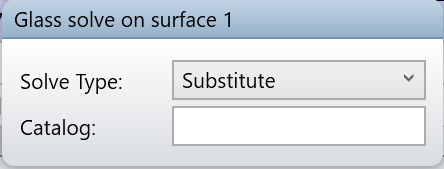
\includegraphics[width=.48\textwidth,height=.24\textheight,keepaspectratio]{Figure/玻璃替换/Picture1zh-cn.png}\hfill
                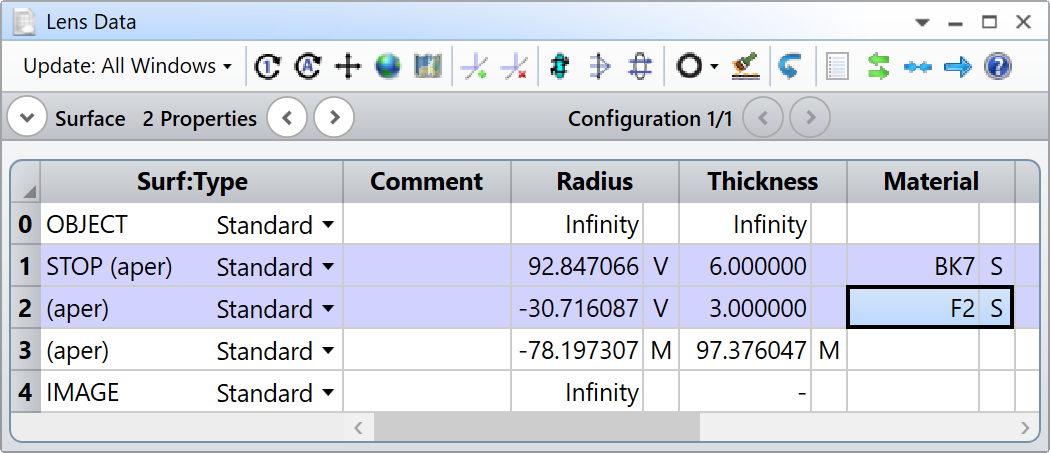
\includegraphics[width=.48\textwidth,height=.24\textheight,keepaspectratio]{Figure/玻璃替换/Picture2zh-cn.png}
                \vspace{4pt}
                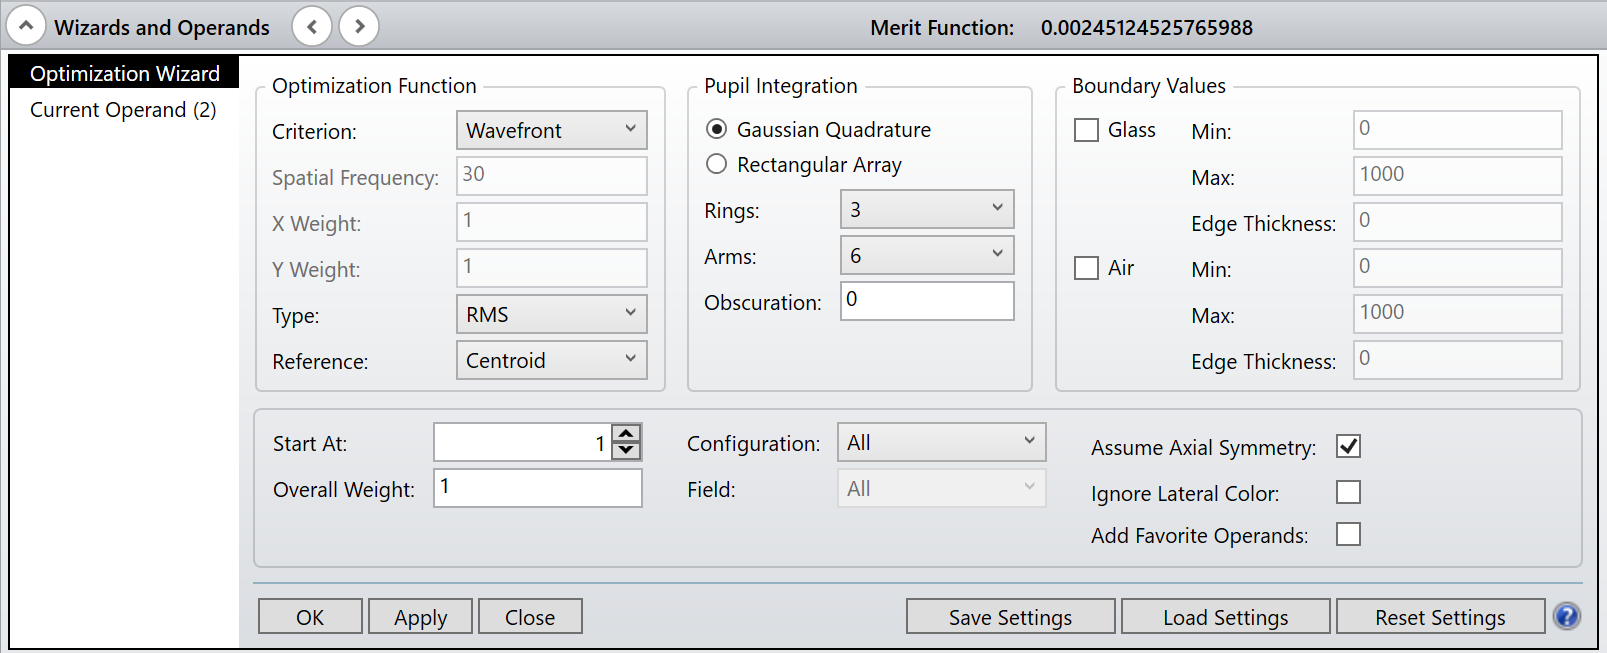
\includegraphics[width=.48\textwidth,height=.24\textheight,keepaspectratio]{Figure/玻璃替换/Picture3zh-cn.png}\hfill
                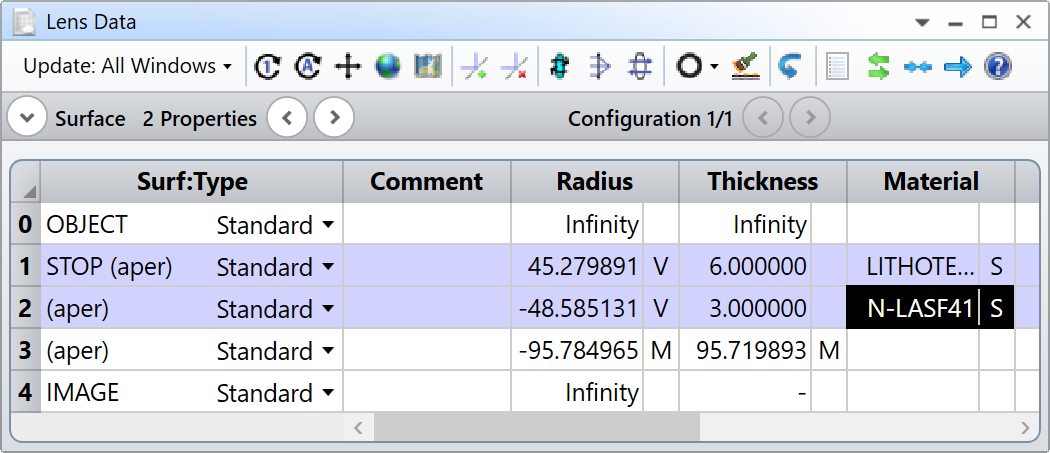
\includegraphics[width=.48\textwidth,height=.24\textheight,keepaspectratio]{Figure/玻璃替换/Picture8zh-cn.png}
                \caption{Substitute solve、评价函数、Hammer 优化与玻璃模板}
                \label{fig:glass_substitution_steps_main}
            \end{figure}
        \end{column}
    \end{columns}
\end{frame}

\subsection{诊断闭环：从图到结论}
\label{sec:1.6}

\englishtitle{Diagnostic Workflow}
\begin{frame}{像差诊断流程：从图到结论}
\label{1.16}
    \begin{columns}[T]
        \begin{column}{.50\textwidth}
            \begin{block}{Ray Fan 先行诊断}
                \begin{enumerate}
                    \item 先看轴上视场：三次曲线为球差，波长斜率差为轴向色差。
                    \item 再看轴外视场：二次曲线为彗差，原点斜率变化为场曲/像散。
                    \item 对比子午和弧矢：斜率分离说明像散。
                    \item 对比不同波长：截距分离说明倍率色差。
                    \item 对比满刻度宽度：光束变窄说明渐晕或光瞳像差。
                \end{enumerate}
            \end{block}
        \end{column}
        \hfill
        \begin{column}{.50\textwidth}
            \begin{block}{再用波前和像质确认}
                \begin{itemize}
                    \item \textbf{Zernike}：分解 OPD，确认主要波前模式。
                    \item \textbf{Spot}：查看几何弥散斑是否落入像元。
                    \item \textbf{PSF}：查看点像能量是否集中。
                    \item \textbf{MTF}：查看目标空间频率的对比度传递。
                    \item \textbf{Encircled Energy}：查看探测器采样能量是否足够。
                \end{itemize}
            \end{block}

            \begin{alertblock}{最重要的工作习惯}
                不要只看一个图下结论；Ray Fan 告诉你“像差形状”，OPD/Zernike 告诉你“波前来源”，MTF/PSF 告诉你“图像后果”。
            \end{alertblock}
        \end{column}
    \end{columns}
\end{frame}

\section{像差类型分析与像质评估}

\subsection{单色像差与矫正方法}

\englishtitle{Characteristics of Spherical Aberration}
\begin{frame}{球差的特征}
    \begin{columns}[T]
        \begin{column}{.45\textwidth}
            \begin{figure}
                \centering
                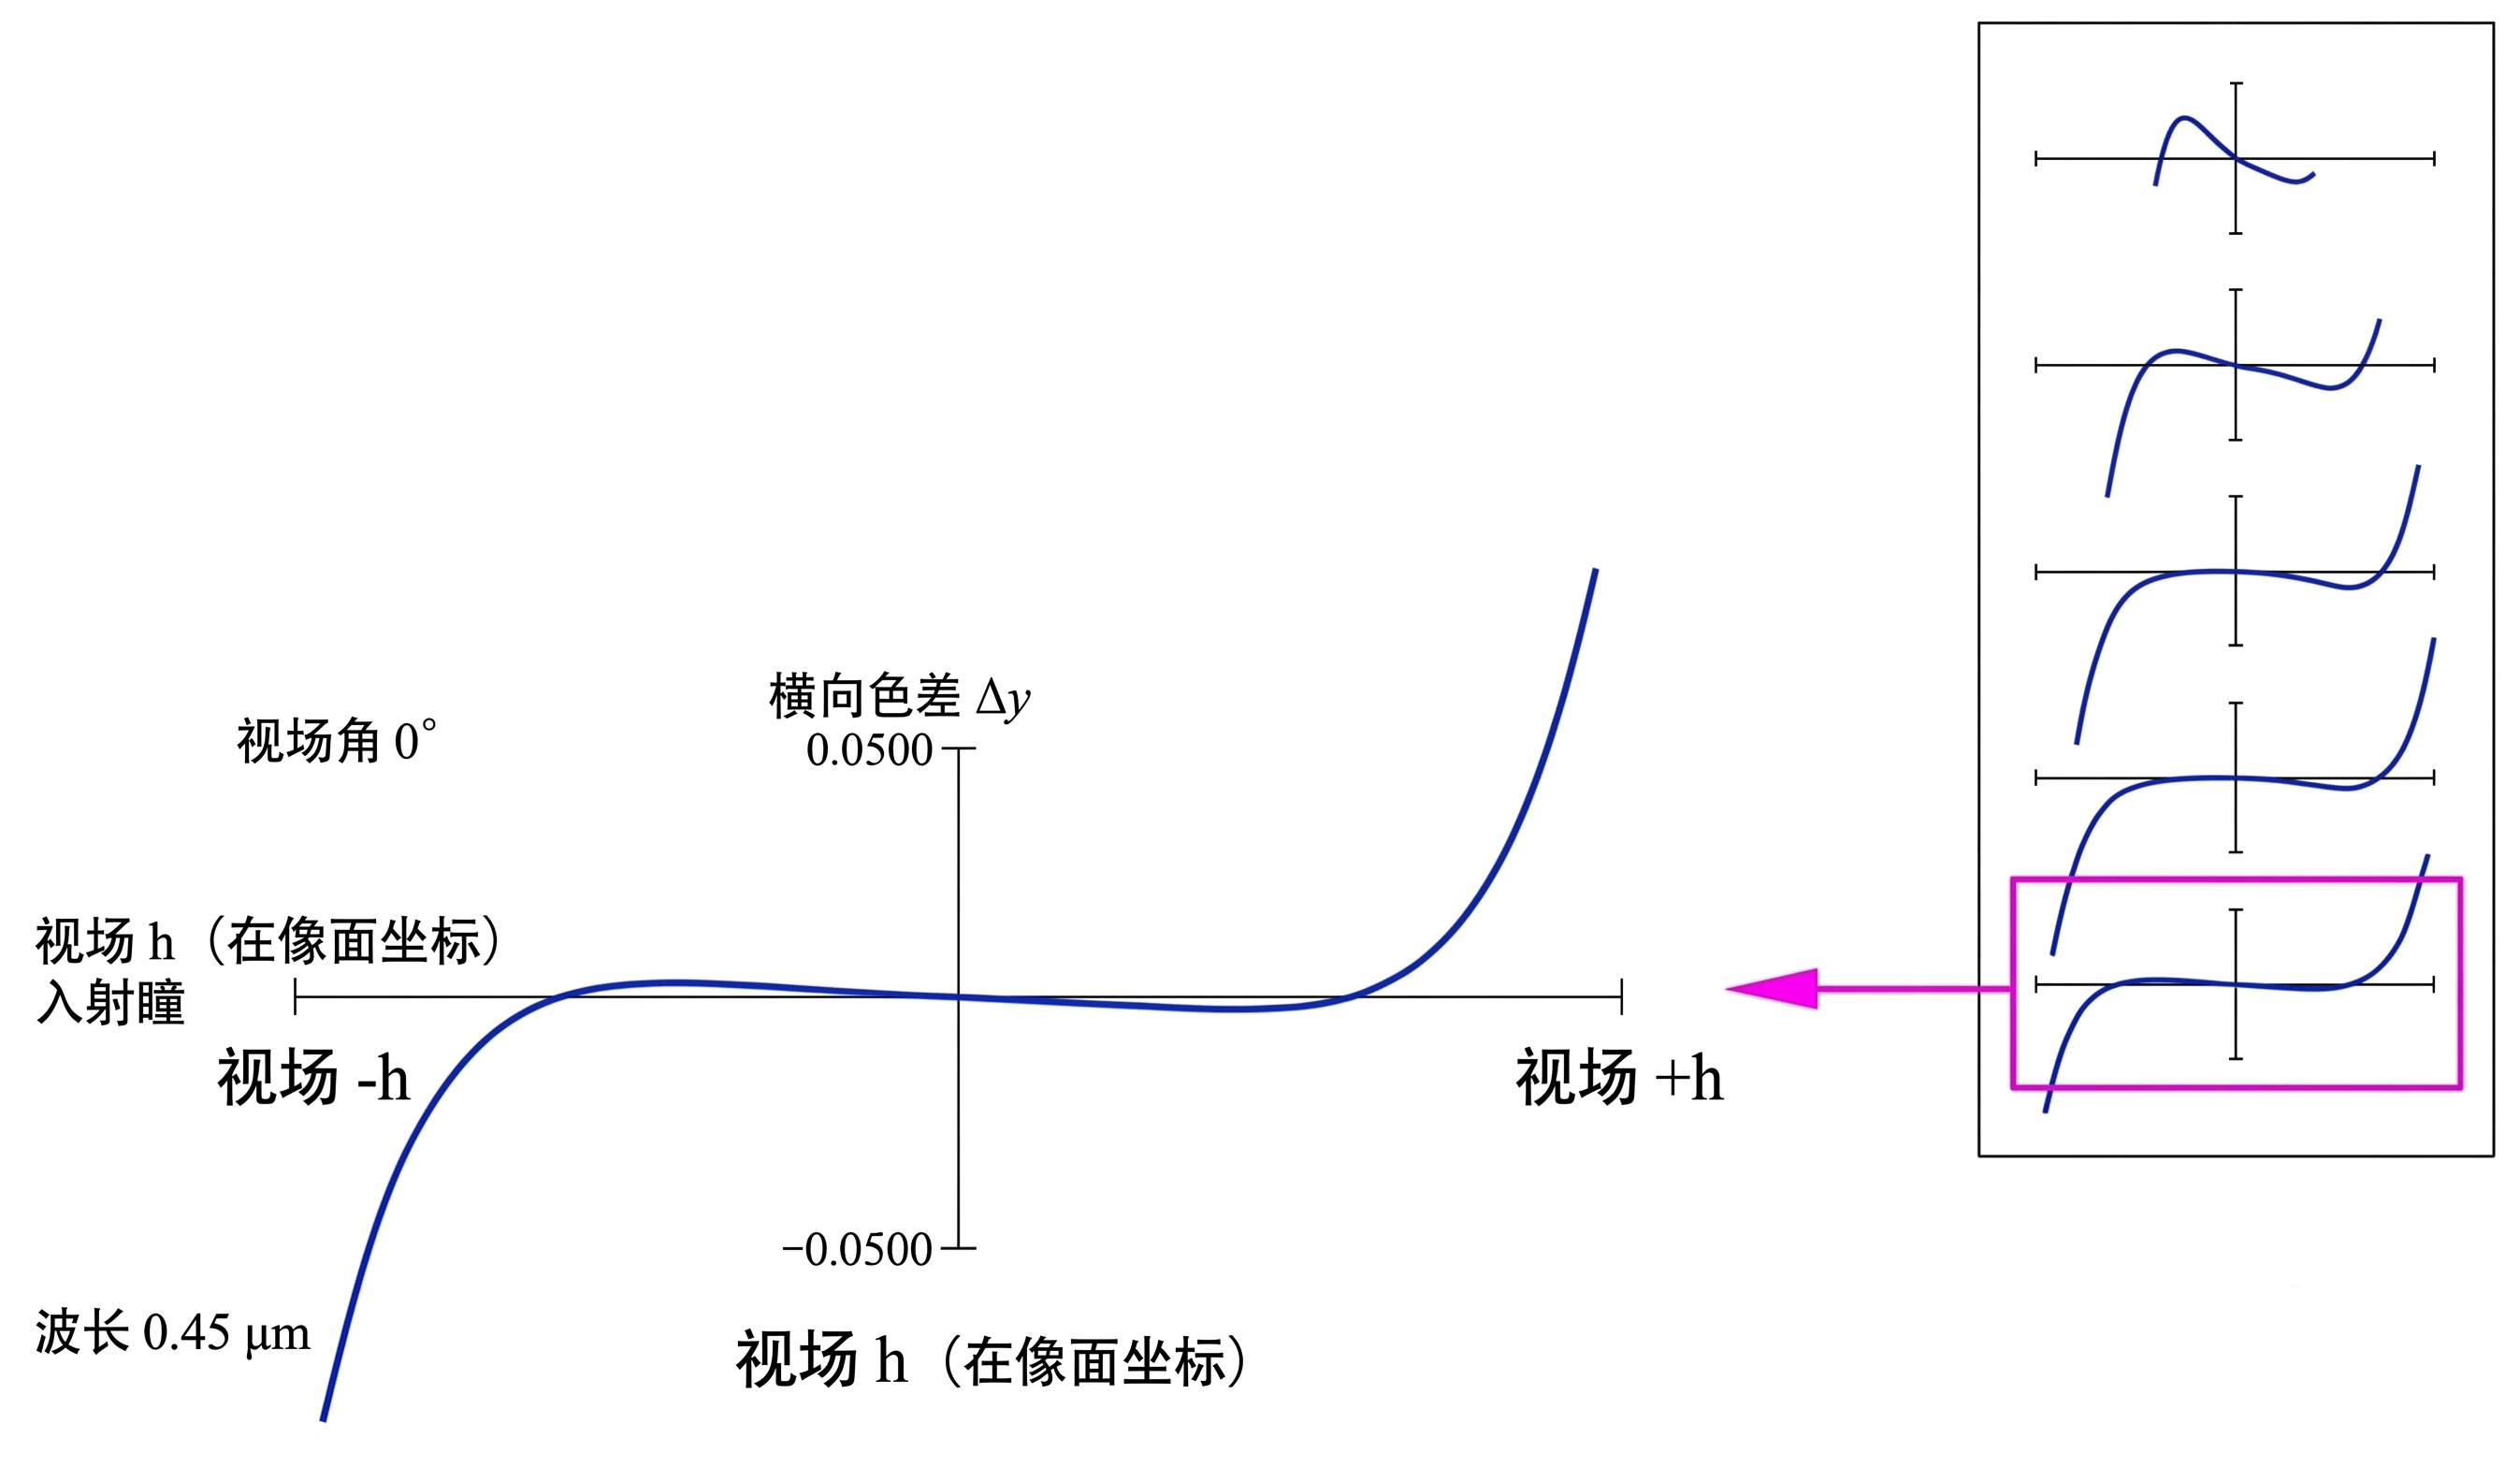
\includegraphics[width=0.95\textwidth]{Figure/图片23.png}
                \caption{球差引起的横向像差图——三次曲线}
                \label{fig:spherical}
            \end{figure}
        \end{column}
        \hfill
        \begin{column}{.55\textwidth}
            \textbf{球差(Spherical Aberration)：}
            \bigbreak
            轴上光束中出现的\alert{唯一单色像差}。与孔径三次方成正比，横向像差图表现为\alert{三次曲线}(奇函数)。可包含3阶、5阶、7阶等奇函数分量。

            \bigbreak
            \textbf{混合像差：}实际系统中球差很少单独出现，通常与离焦分量和高阶球差混合。

            \bigbreak
            \alert{需要将各成分分解分析，才能有效优化镜头性能。}
        \end{column}
    \end{columns}
\end{frame}

\englishtitle{Correction Methods for Spherical Aberration}
\begin{frame}{球差矫正方法}
    \begin{block}{球差的定义}
        轴上光线与边缘光线在光轴上焦点之间的\alert{轴向距离}即为球差。
    \end{block}

    \textbf{主要矫正策略：}
    \begin{enumerate}
        \item \alert{分摊光焦度}：将单个透镜的光焦度分配给多个透镜，减小每个面的曲率
        \item \alert{透镜拆分}：用大曲率半径的多个透镜替代小曲率半径的单一透镜
        \item \alert{胶合透镜}：利用正负透镜的球差符号相反进行相互抵消
        \item \alert{非球面透镜}：通过改变面形消除球差(最理想方式)
    \end{enumerate}

    \alert{核心思路：}球差源于球面折射面的几何形状，通过改变面形或光焦度分配来减小不同孔径区域的折射角度差异。
\end{frame}

\englishtitle{Characteristics and Types of Coma}
\begin{frame}{彗差的特征与类型}
    \begin{columns}[T,onlytextwidth]
        \begin{column}{.55\textwidth}
            \begin{block}{\footnotesize 光路图与横向像差图对比}
                \centering
                \begin{minipage}[t]{.49\linewidth}
                    \centering
                    {\scriptsize \alert{外向彗差}}
                    \par\vspace{2pt}
                    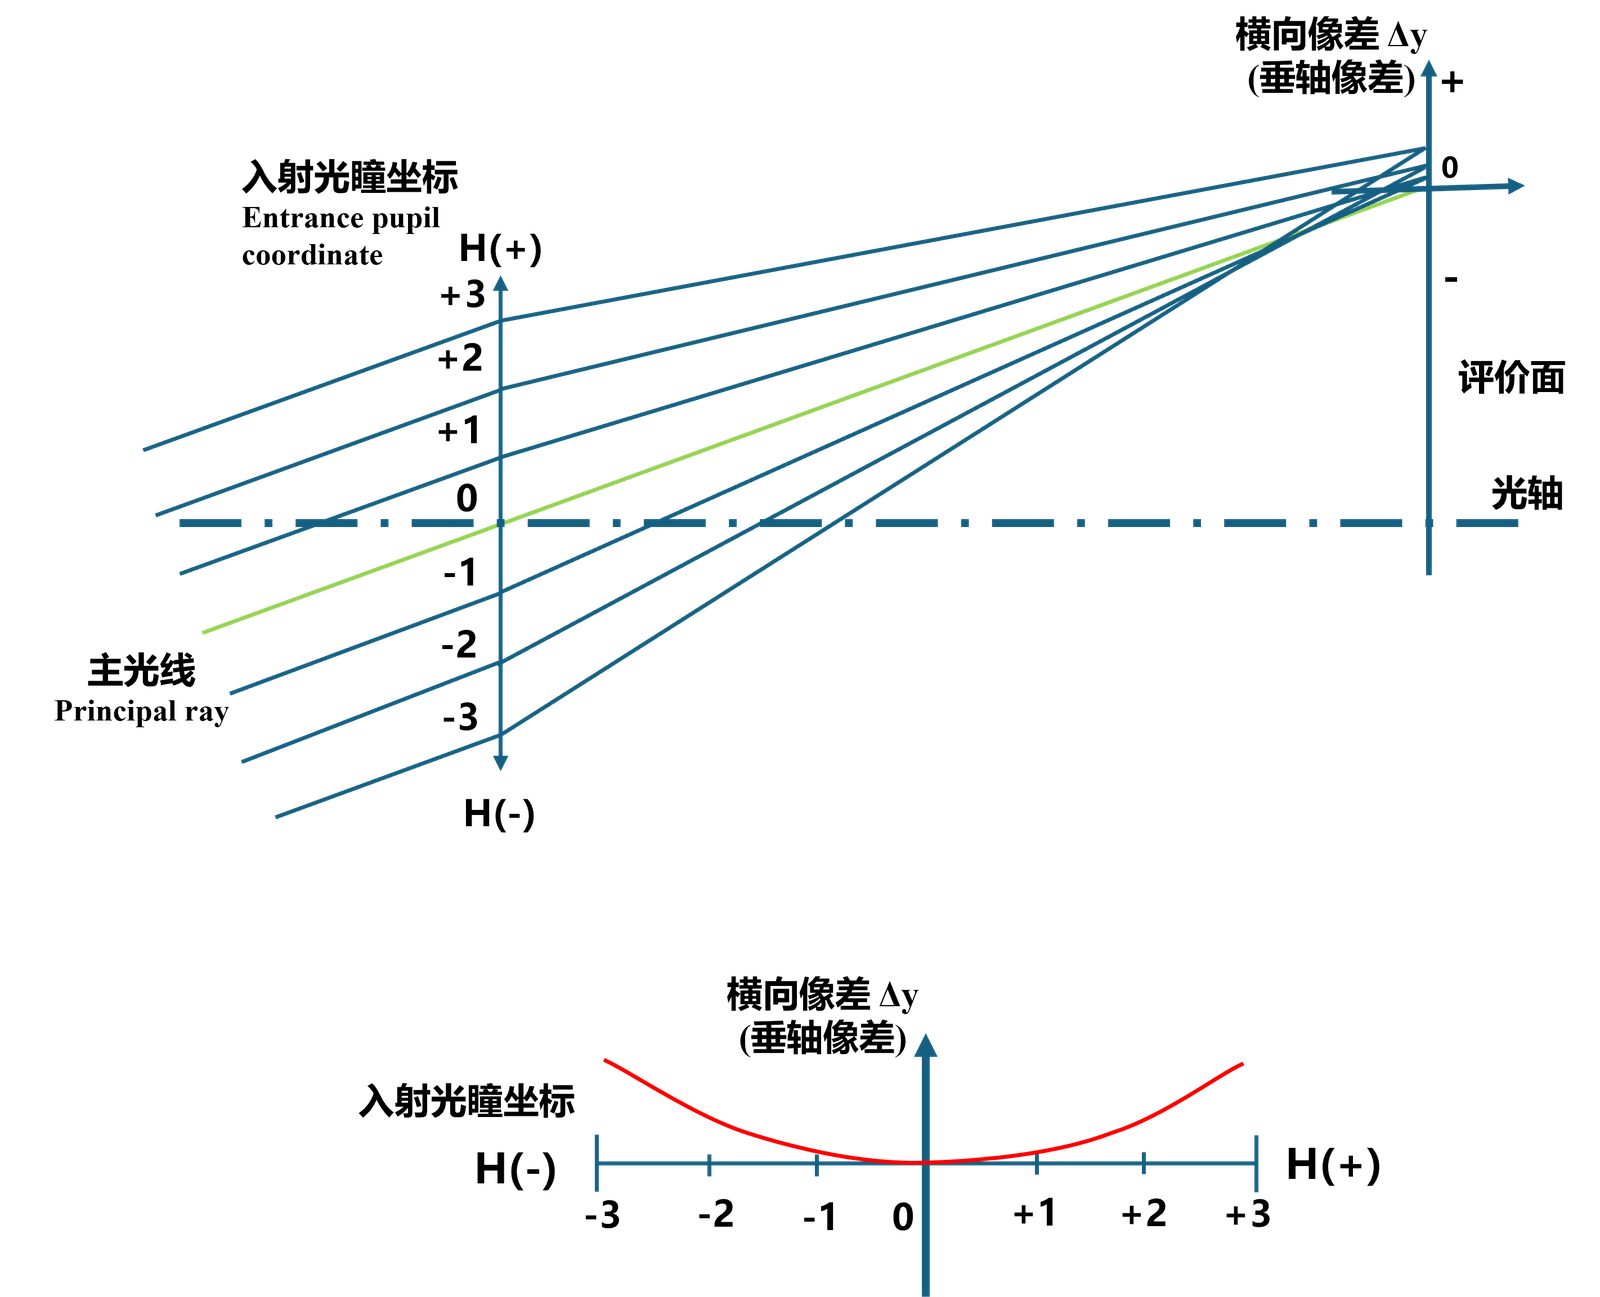
\includegraphics[width=\linewidth,height=.34\textheight,keepaspectratio]{Figure/图片8.png}
                    \par\vspace{2pt}
                    {\scriptsize 下凸二次曲线}
                    \label{fig:outward_coma}
                \end{minipage}
                \hfill
                \begin{minipage}[t]{.49\linewidth}
                    \centering
                    {\scriptsize \alert{内向彗差}}
                    \par\vspace{2pt}
                    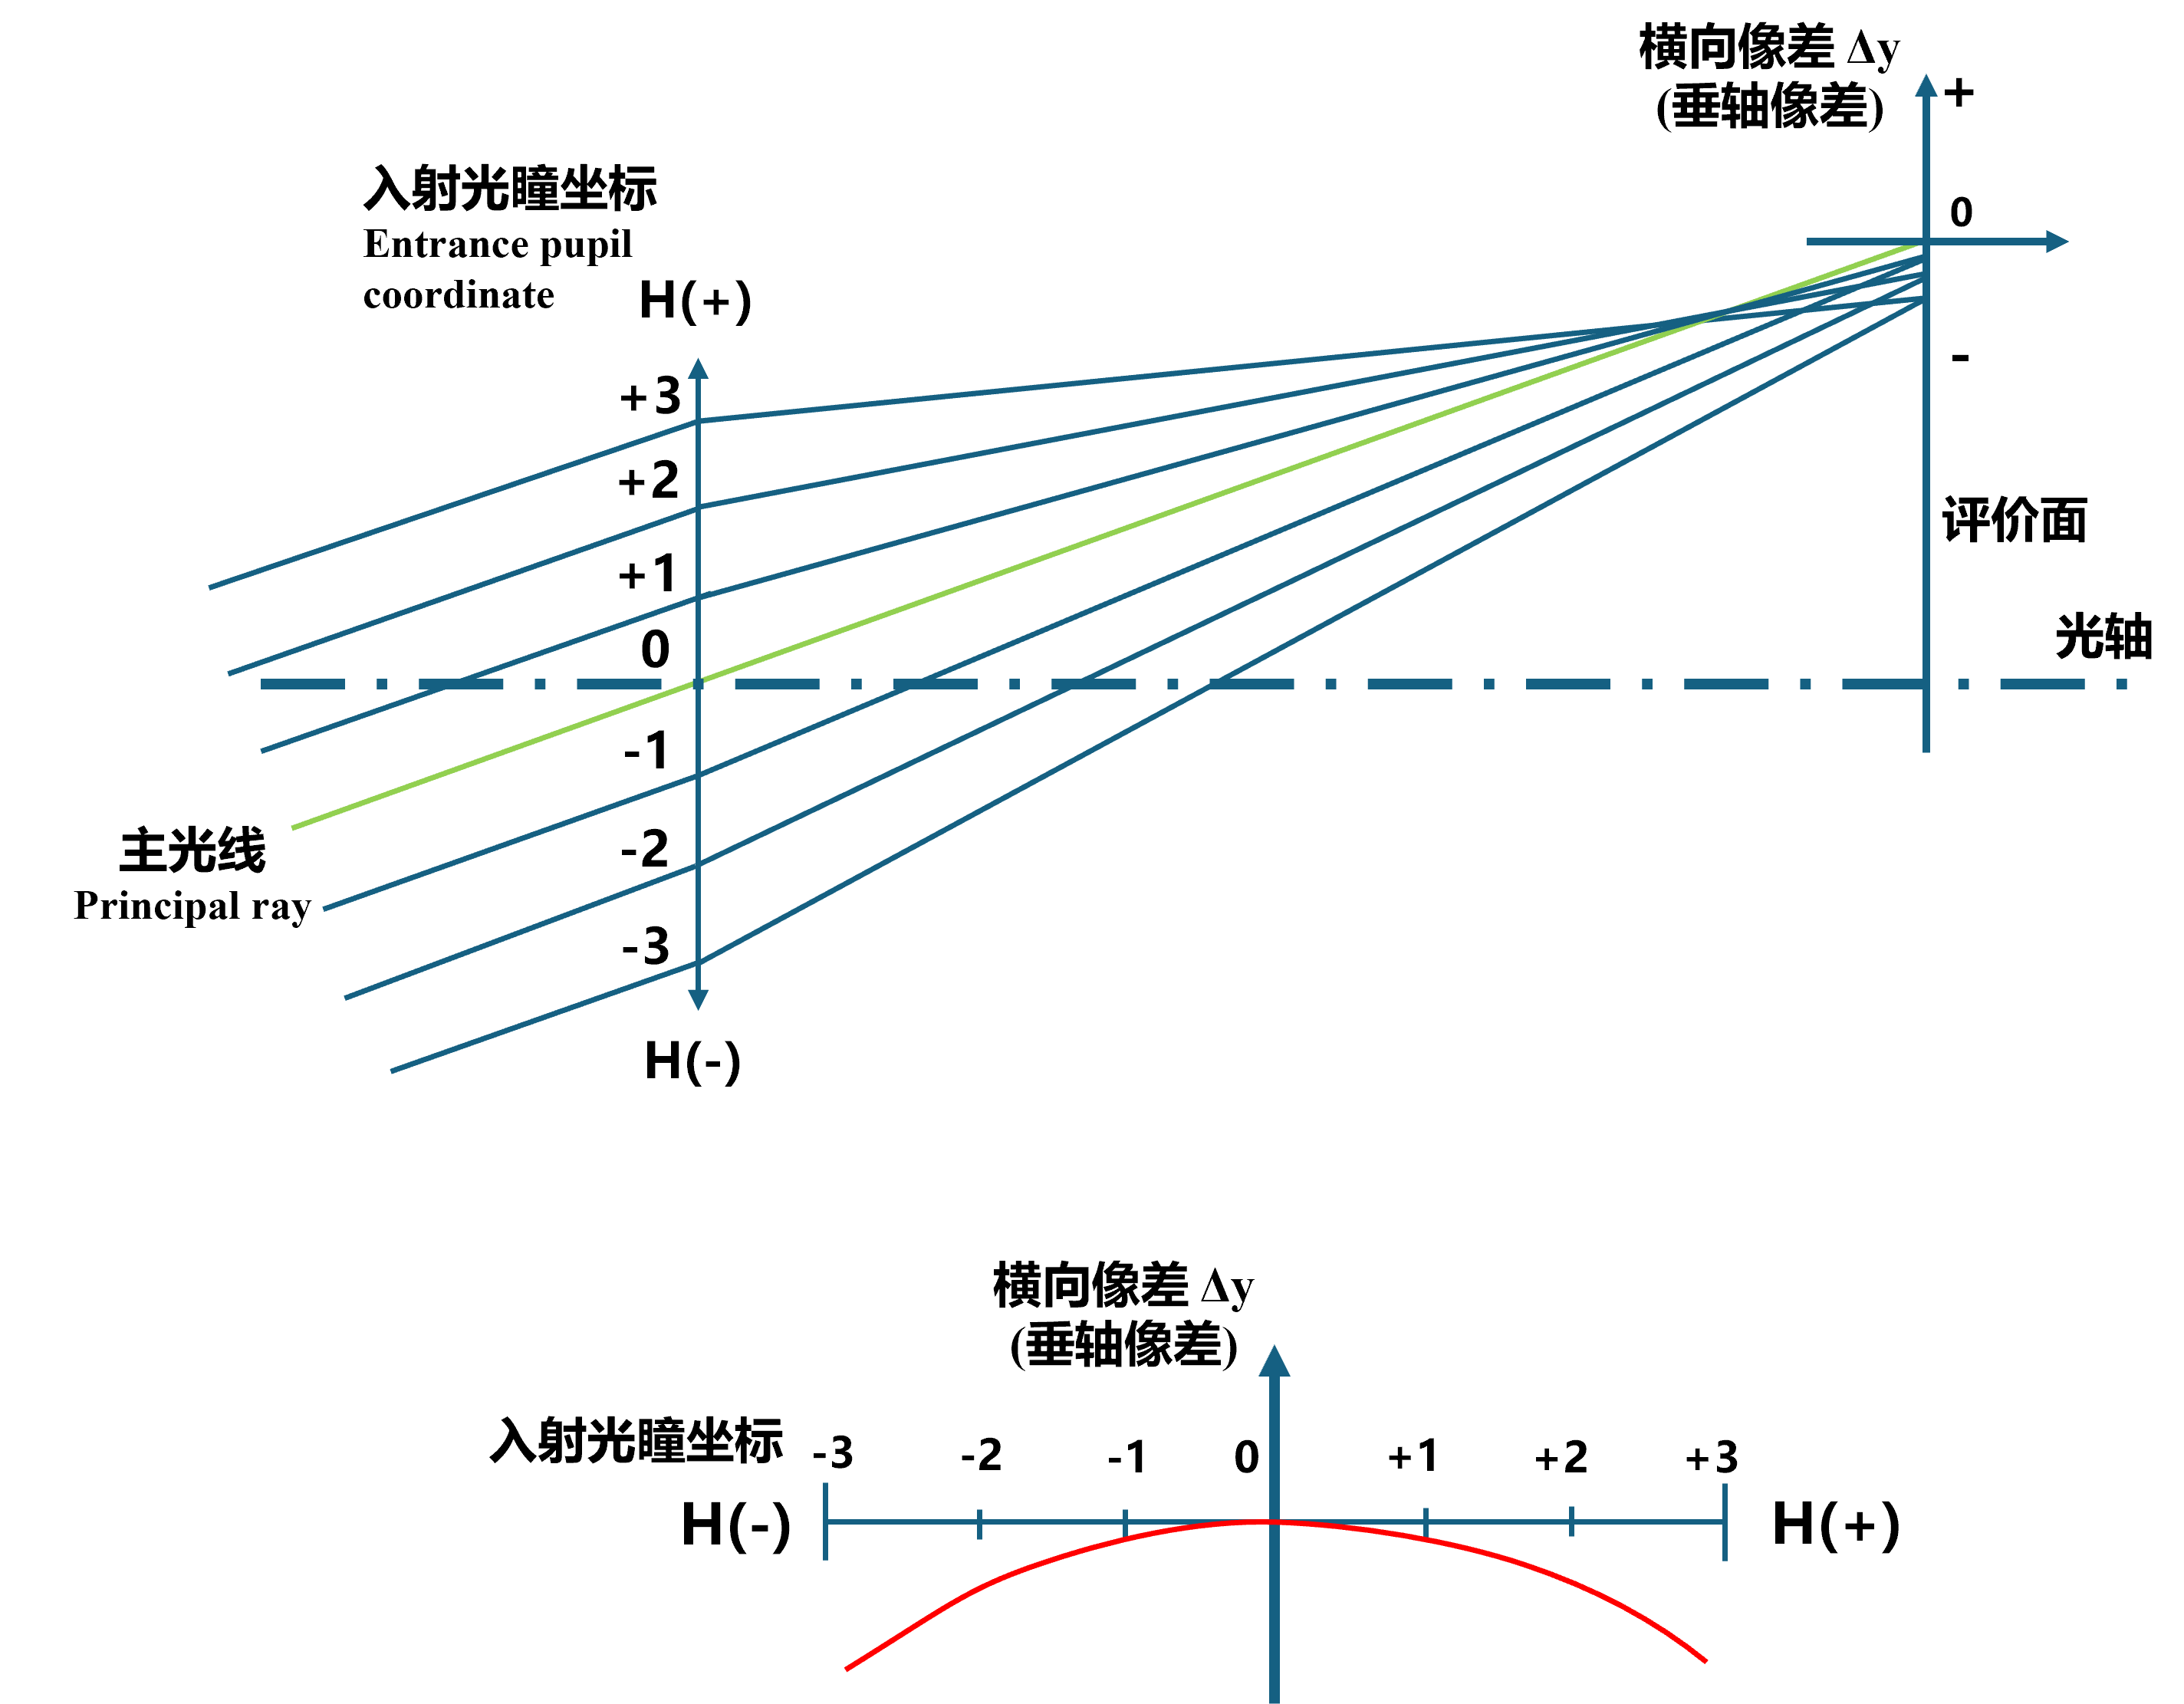
\includegraphics[width=\linewidth,height=.34\textheight,keepaspectratio]{Figure/图片11.png}
                    \par\vspace{2pt}
                    {\scriptsize 上凸二次曲线}
                    \label{fig:inward_coma}
                \end{minipage}
            \end{block}
        \end{column}
        \hfill
        \begin{column}{.43\textwidth}
            \begin{block}{\footnotesize 彗差的定义}
                \small
                横向像差图关于入射光瞳坐标呈\alert{二次函数关系}的像差。与 $h^2$ 成正比(偶函数)。
            \end{block}

            \vspace{2pt}
            \small
            \textbf{两种类型及判断：}
            \begin{enumerate}
                \setlength{\itemsep}{3pt}
                \item \alert{外向彗差}：\alert{下凸}二次曲线
                \begin{itemize}
                    \setlength{\itemsep}{-1pt}
                    \item 上侧光线穿过主光线后落在正侧
                \end{itemize}
                \item \alert{内向彗差}：\alert{上凸}二次曲线
                \begin{itemize}
                    \setlength{\itemsep}{-1pt}
                    \item 上侧光线与主光线交叉后落在负侧
                \end{itemize}
            \end{enumerate}

            \vspace{2pt}
            {\small \alert{要点：}看横向像差曲线的开口方向，而不是只看光线图的倾斜程度。}
        \end{column}
    \end{columns}
\end{frame}

\englishtitle{Coma Diagnosis and Correction}
\begin{frame}{彗差判断与矫正}
    \begin{columns}[T]
        \begin{column}{.50\textwidth}
            \textbf{如何判断彗差：}
            \begin{itemize}
                \item 横向像差图呈 $\propto h^2$ 的二次曲线
                \item 下凸 $\rightarrow$ 外向彗差 / 上凸 $\rightarrow$ 内向彗差
                \item 离焦\alert{无法改善}彗差——这是区分彗差与离焦的关键
                \item 彗差属偶函数，球差属奇函数
            \end{itemize}
        \end{column}
        \hfill
        \begin{column}{.50\textwidth}
            \textbf{彗差矫正策略：}
            \begin{enumerate}
                \item \alert{改变光阑位置}：满足阿贝正弦条件
                \item \alert{非球面透镜}：改变轴外光线折射角分布
                \item \alert{对称光学结构}：前后对称抵消奇次彗差
            \end{enumerate}

            \alert{注意：}彗差本质是\alert{轴外球差}，在\alert{大孔径+大视场}时最严重。
        \end{column}
    \end{columns}
\end{frame}

\englishtitle{Hidden Coma}
\begin{frame}{隐性彗差}
    \begin{columns}[T]
        \begin{column}{.50\textwidth}
            \begin{figure}
                \centering
                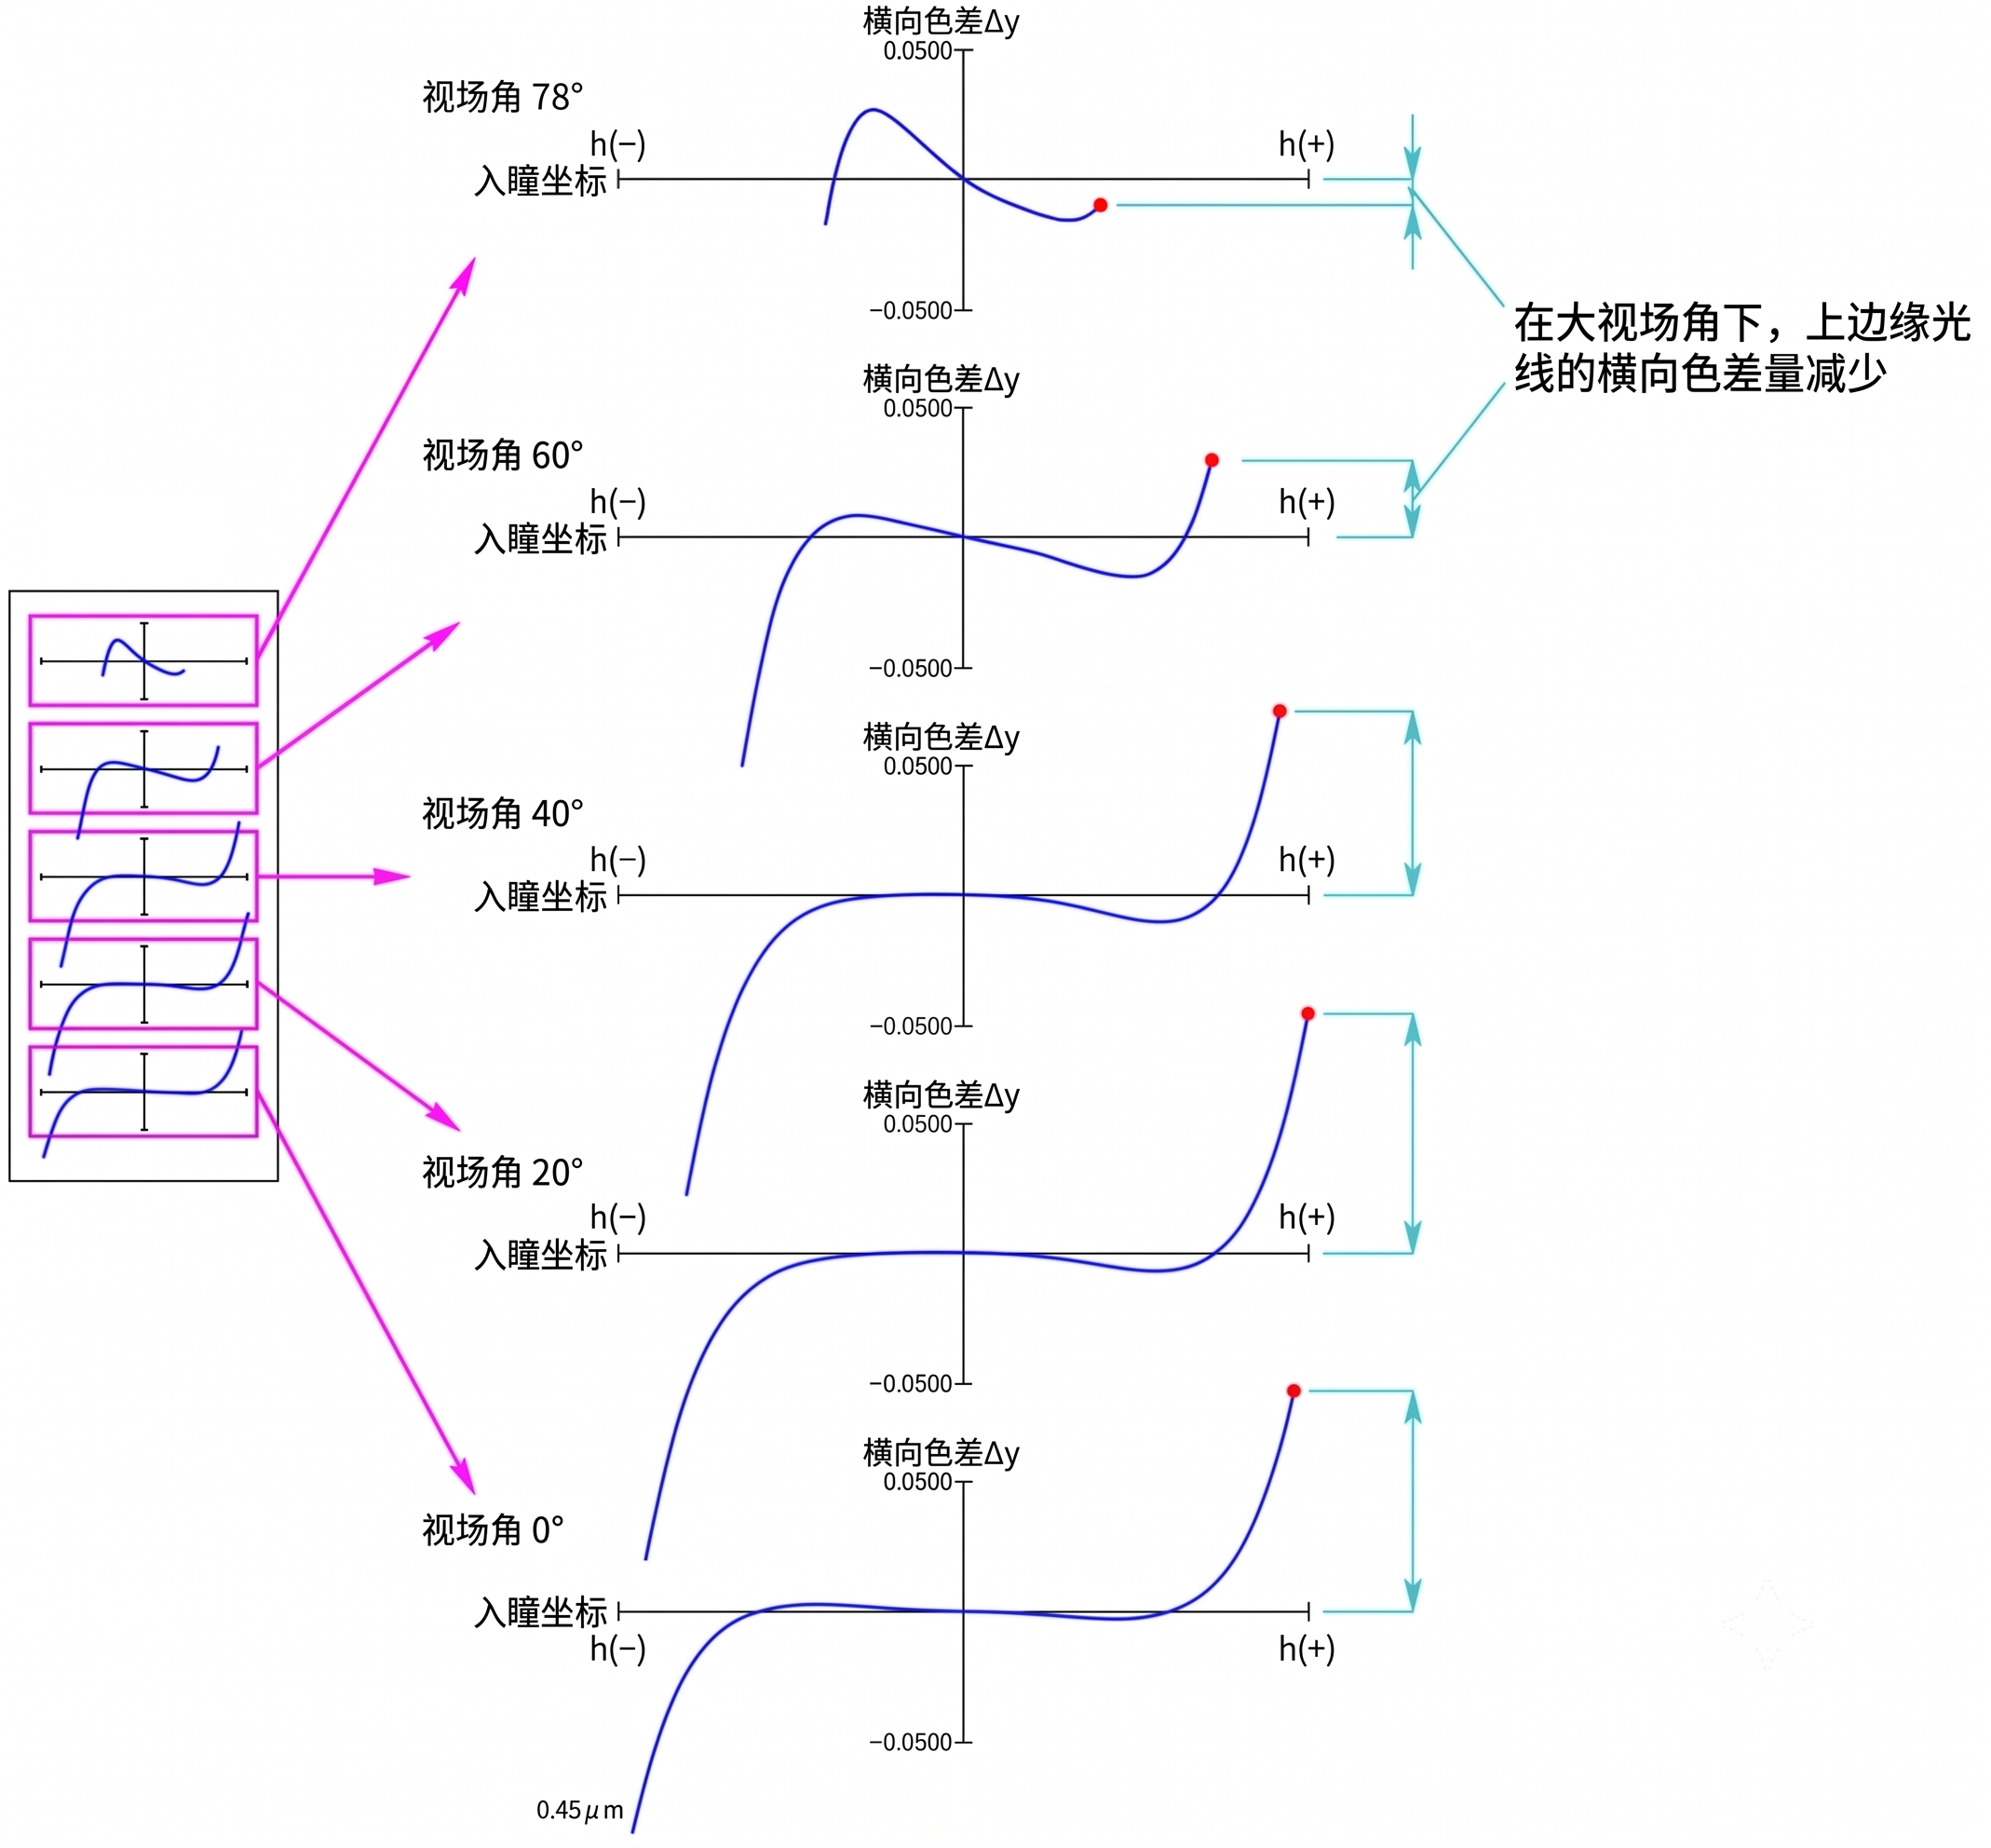
\includegraphics[width=0.9\textwidth]{Figure/图片24.png}
                \caption{隐性彗差——上边缘光线随视场增大而减小}
                \label{fig:hidden_coma}
            \end{figure}
        \end{column}
        \hfill
        \begin{column}{.50\textwidth}
            典型光学系统中，横向像差包含\alert{离焦、球差、彗差和场曲}的复合分量。

            \bigbreak
            \textbf{隐性彗差的特征：}
            \begin{itemize}
                \item 上边缘光线像差随视场增大而\alert{减小}
                \item 下边缘光线像差\alert{基本不变}
                \item 球差(奇函数)和彗差(偶函数)叠加
            \end{itemize}

            \bigbreak
            \textbf{机制：}上边缘二者\alert{抵消}，下边缘二者\alert{加强}。
        \end{column}
    \end{columns}
\end{frame}

\englishtitle{Transverse Aberration of Field Curvature}
\begin{frame}{场曲的横向像差图特征}
    \begin{columns}[T]
        \begin{column}{.35\textwidth}
            \begin{figure}
                \centering
                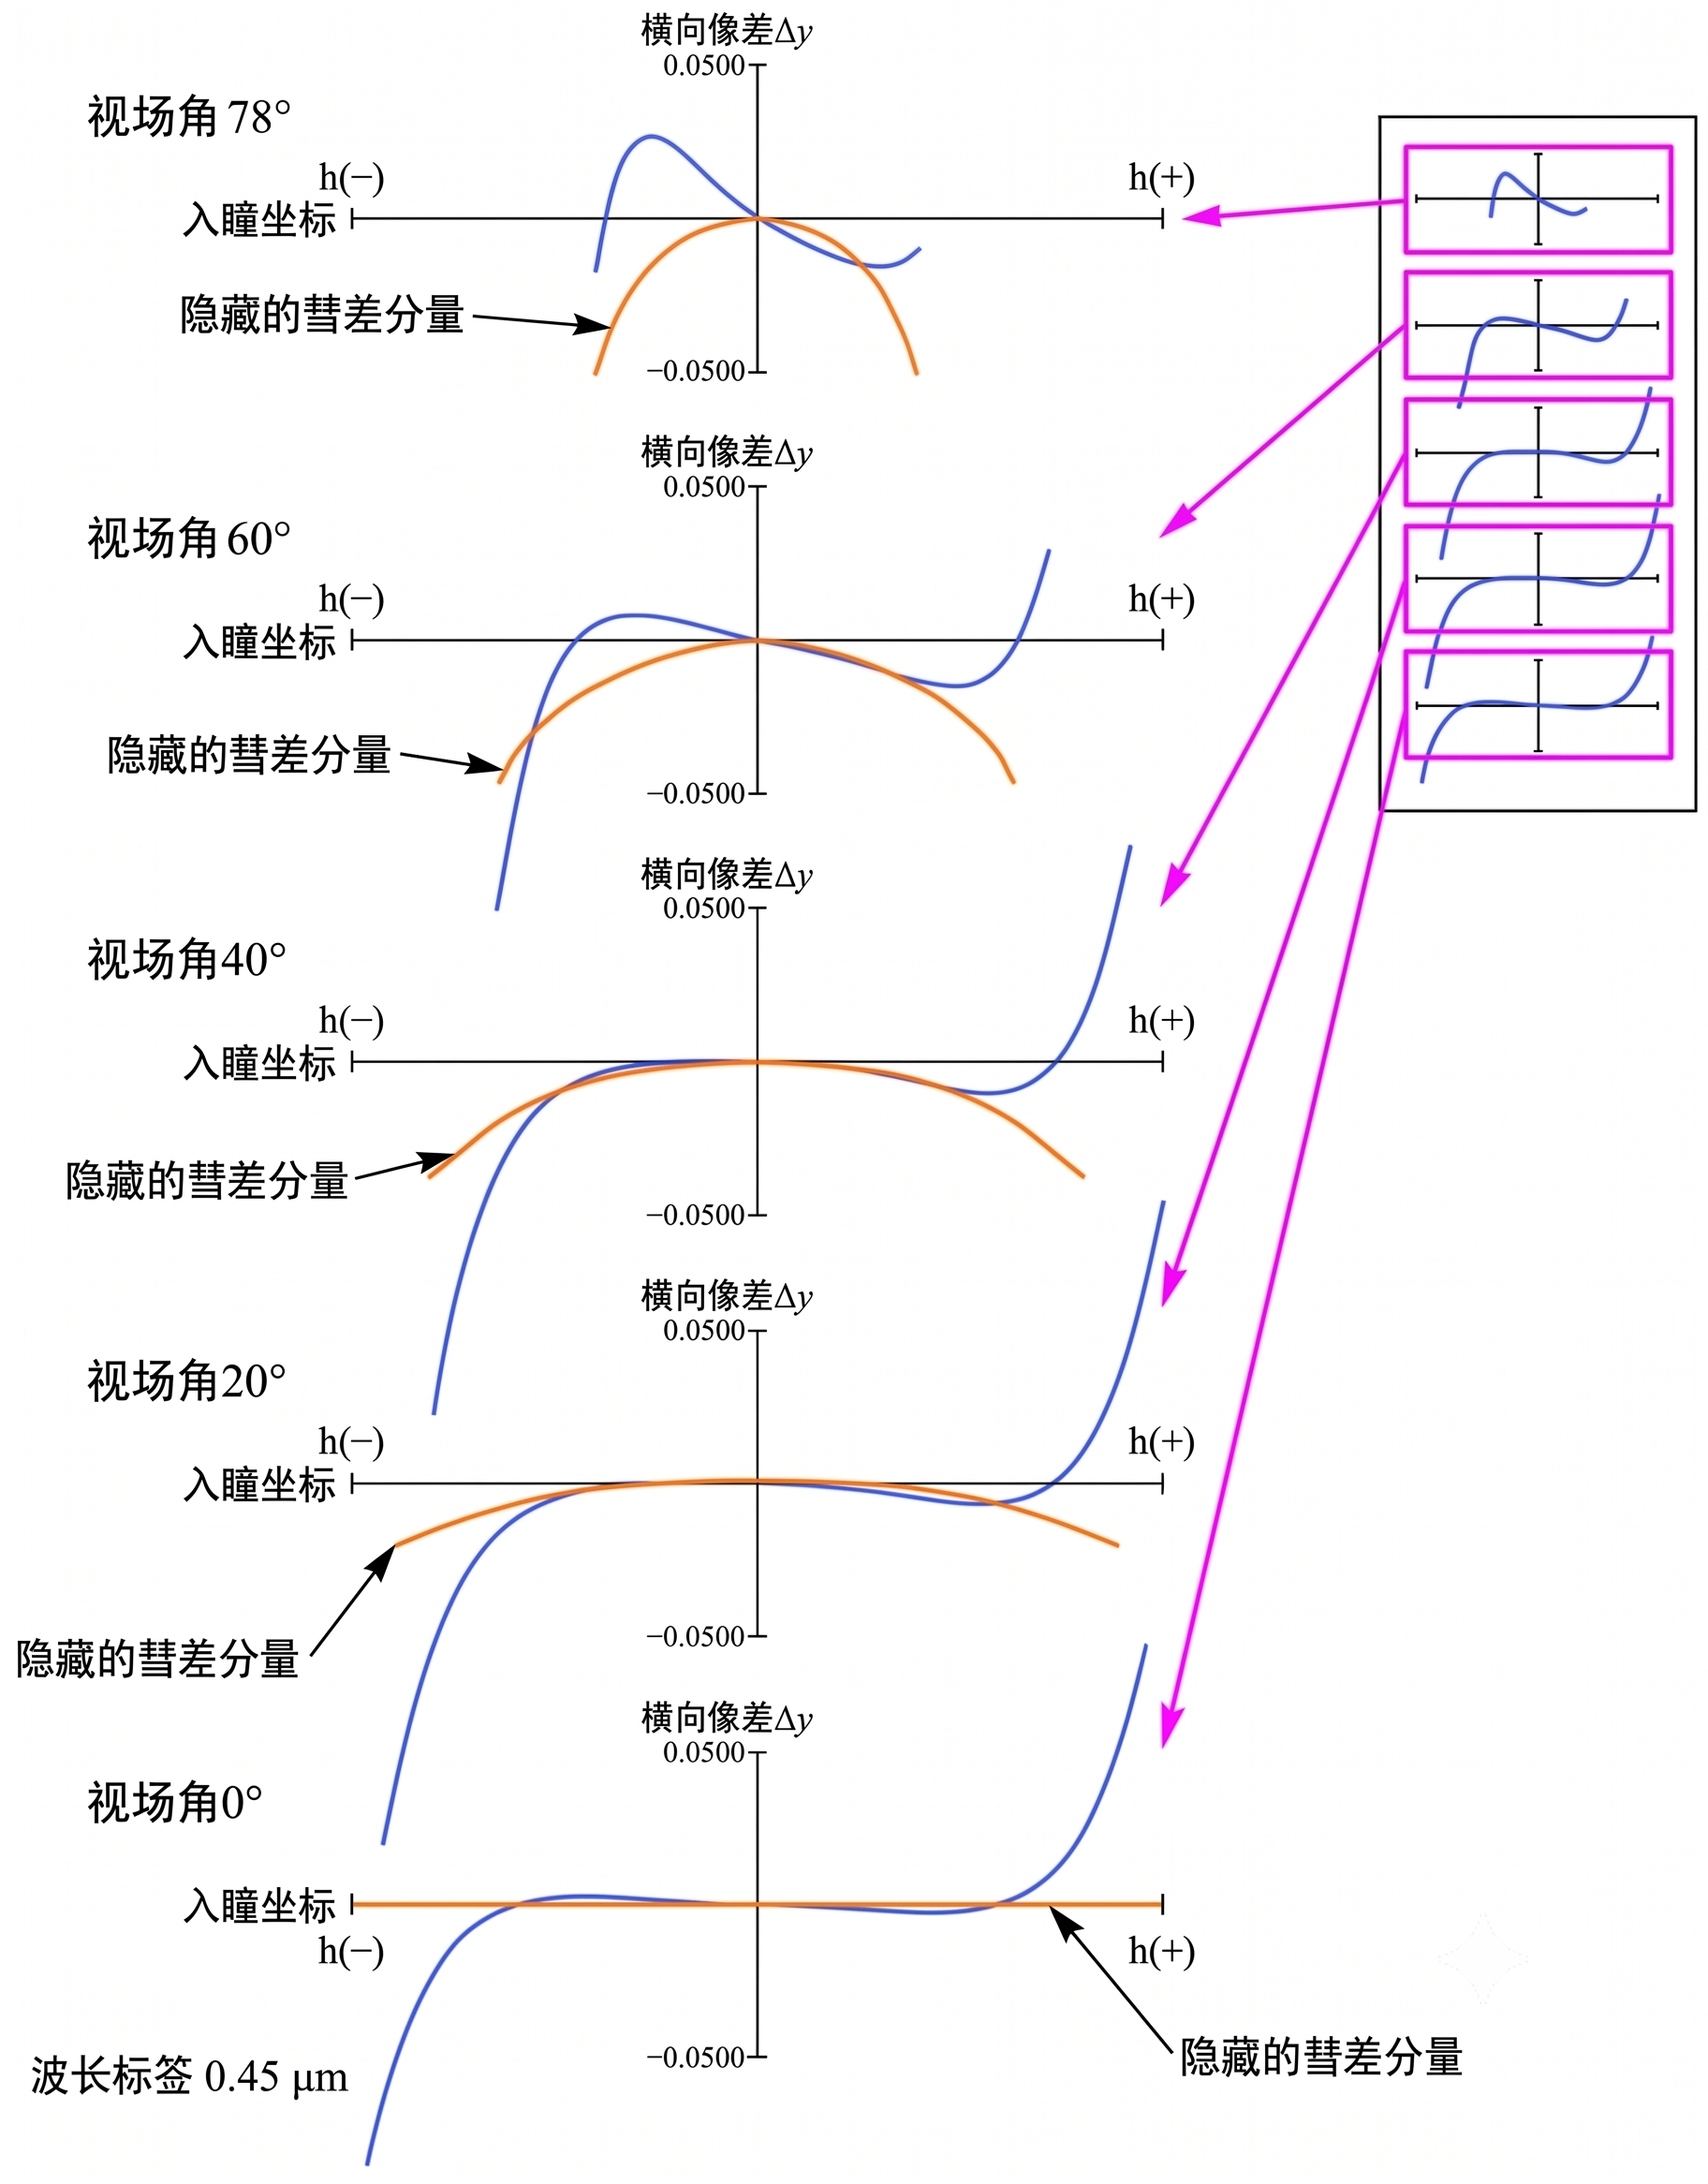
\includegraphics[width=0.9\textwidth]{Figure/图片25.png}
                \caption{场曲——原点附近斜率因视场而异}
                \label{fig:field_curvature}
            \end{figure}
        \end{column}
        \hfill
        \begin{column}{.65\textwidth}
            \textbf{场曲(Field Curvature)：}
            即使物面是平面，像面也可能弯曲——\alert{场曲}。

            \bigbreak
            \textbf{识别方法：}横向像差图\alert{原点附近}斜率因视场角不同而不同。

            \bigbreak
            各视场成像点在纵向上\alert{不同}，连接后形成\alert{弯曲的像面}(Petzval曲面)。

            \bigbreak
            \textbf{为何关注原点附近？}
            \begin{itemize}
                \item 球差($h^3$)和彗差($h^2$)在此处影响极小
                \item 场曲($h^1$)在原点附近\alert{占主导}
            \end{itemize}
        \end{column}
    \end{columns}
\end{frame}

\englishtitle{Correction Methods for Field Curvature}
\begin{frame}{场曲矫正方法}
    \begin{columns}[T]
        \begin{column}{.52\textwidth}
            \textbf{佩兹伐和(Petzval Sum)控制：}
            场曲受系统的佩兹伐和支配，核心是\alert{降低总佩兹伐和}。

            \textbf{主要策略：}
            \begin{enumerate}
                \item \alert{正负光焦度分离}：正负透镜组合抵消佩兹伐贡献
                \item \alert{弯月透镜}：特殊面形引入负佩兹伐贡献
                \item \alert{场镜}：在像面前改变会聚角而不影响总光焦度
            \end{enumerate}
        \end{column}
        \hfill
        \begin{column}{.48\textwidth}
            \begin{block}{佩兹伐条件(薄透镜)}
                \begin{equation}
                    \sum \frac{\phi_i}{n_i} \rightarrow 0
                    \label{eq:petzval}
                \end{equation}
                其中 $\phi_i$ 为光焦度，$n_i$ 为折射率。

                正负透镜组合是\alert{唯一}能同时校正场曲和维持总光焦度的手段。
            \end{block}
        \end{column}
    \end{columns}
\end{frame}

\englishtitle{Meridional Plane, Sagittal Plane and Astigmatism}
\begin{frame}{子午面、弧矢面与像散}
    \begin{columns}[T]
        \begin{column}{.42\textwidth}
            \begin{figure}
                \centering
                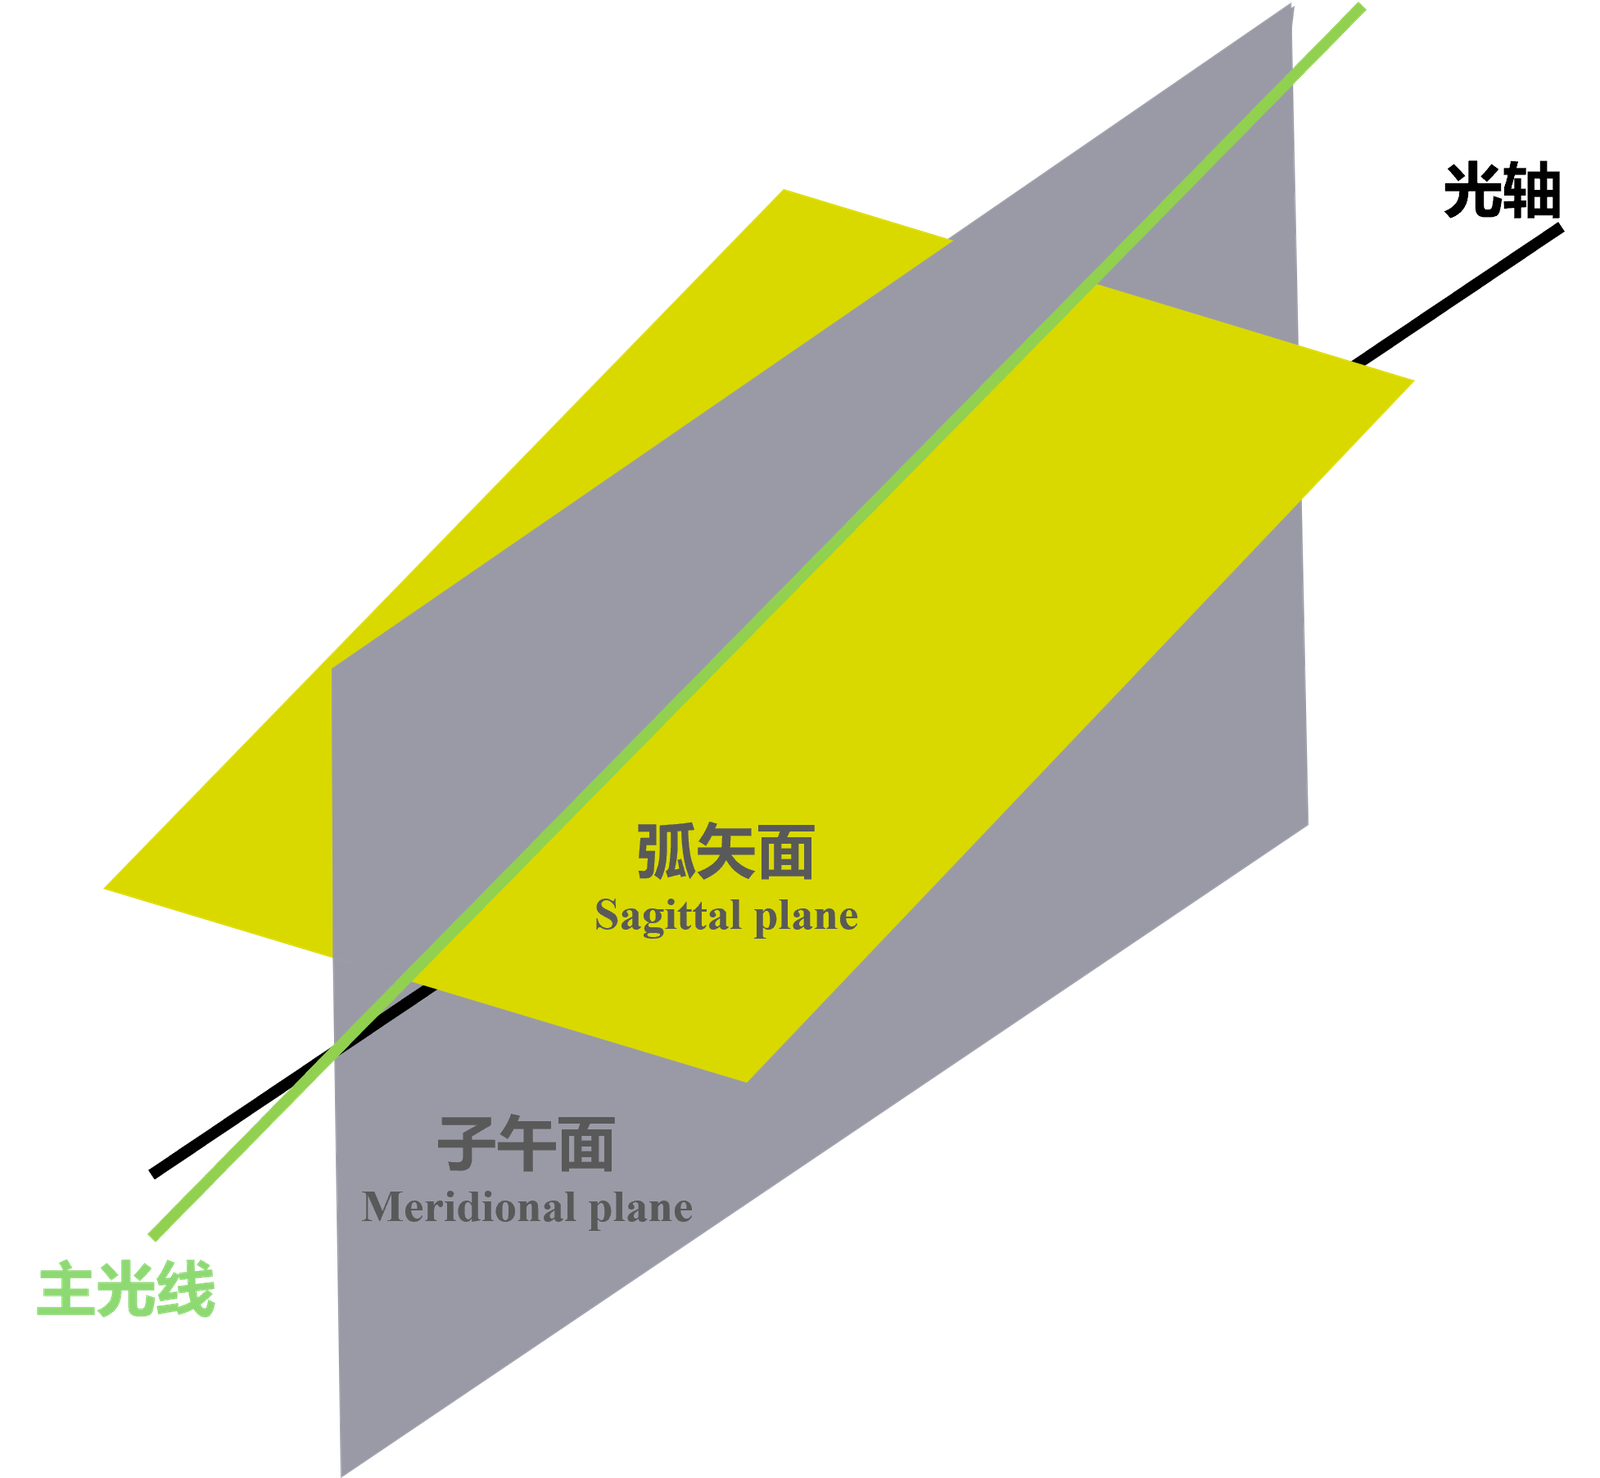
\includegraphics[width=0.9\textwidth]{Figure/图片18.png}
                \caption{子午面和弧矢面的示意图}
                \label{fig:meridional_sagittal}
            \end{figure}
        \end{column}
        \hfill
        \begin{column}{.58\textwidth}
            \begin{itemize}
                \item \textbf{子午面：}包含物点和光轴的平面
                \item \textbf{弧矢面：}垂直于子午面且包含主光线的平面
            \end{itemize}

            \bigbreak
            \textbf{像散(Astigmatism)：}
            即使同视场角，原点附近斜率在子午面和弧矢面之间\alert{不同}——子午和弧矢成像位置不一致。

            \bigbreak
            像散乃\alert{场曲的子午分量和弧矢分量分离}的状态。两个聚焦面上均呈现\alert{线像}而非点像。
        \end{column}
    \end{columns}
\end{frame}

\englishtitle{Astigmatism: Imaging and Correction}
\begin{frame}{像散成像与矫正}
    \begin{columns}[T]
        \begin{column}{.50\textwidth}
            \begin{figure}
                \centering
                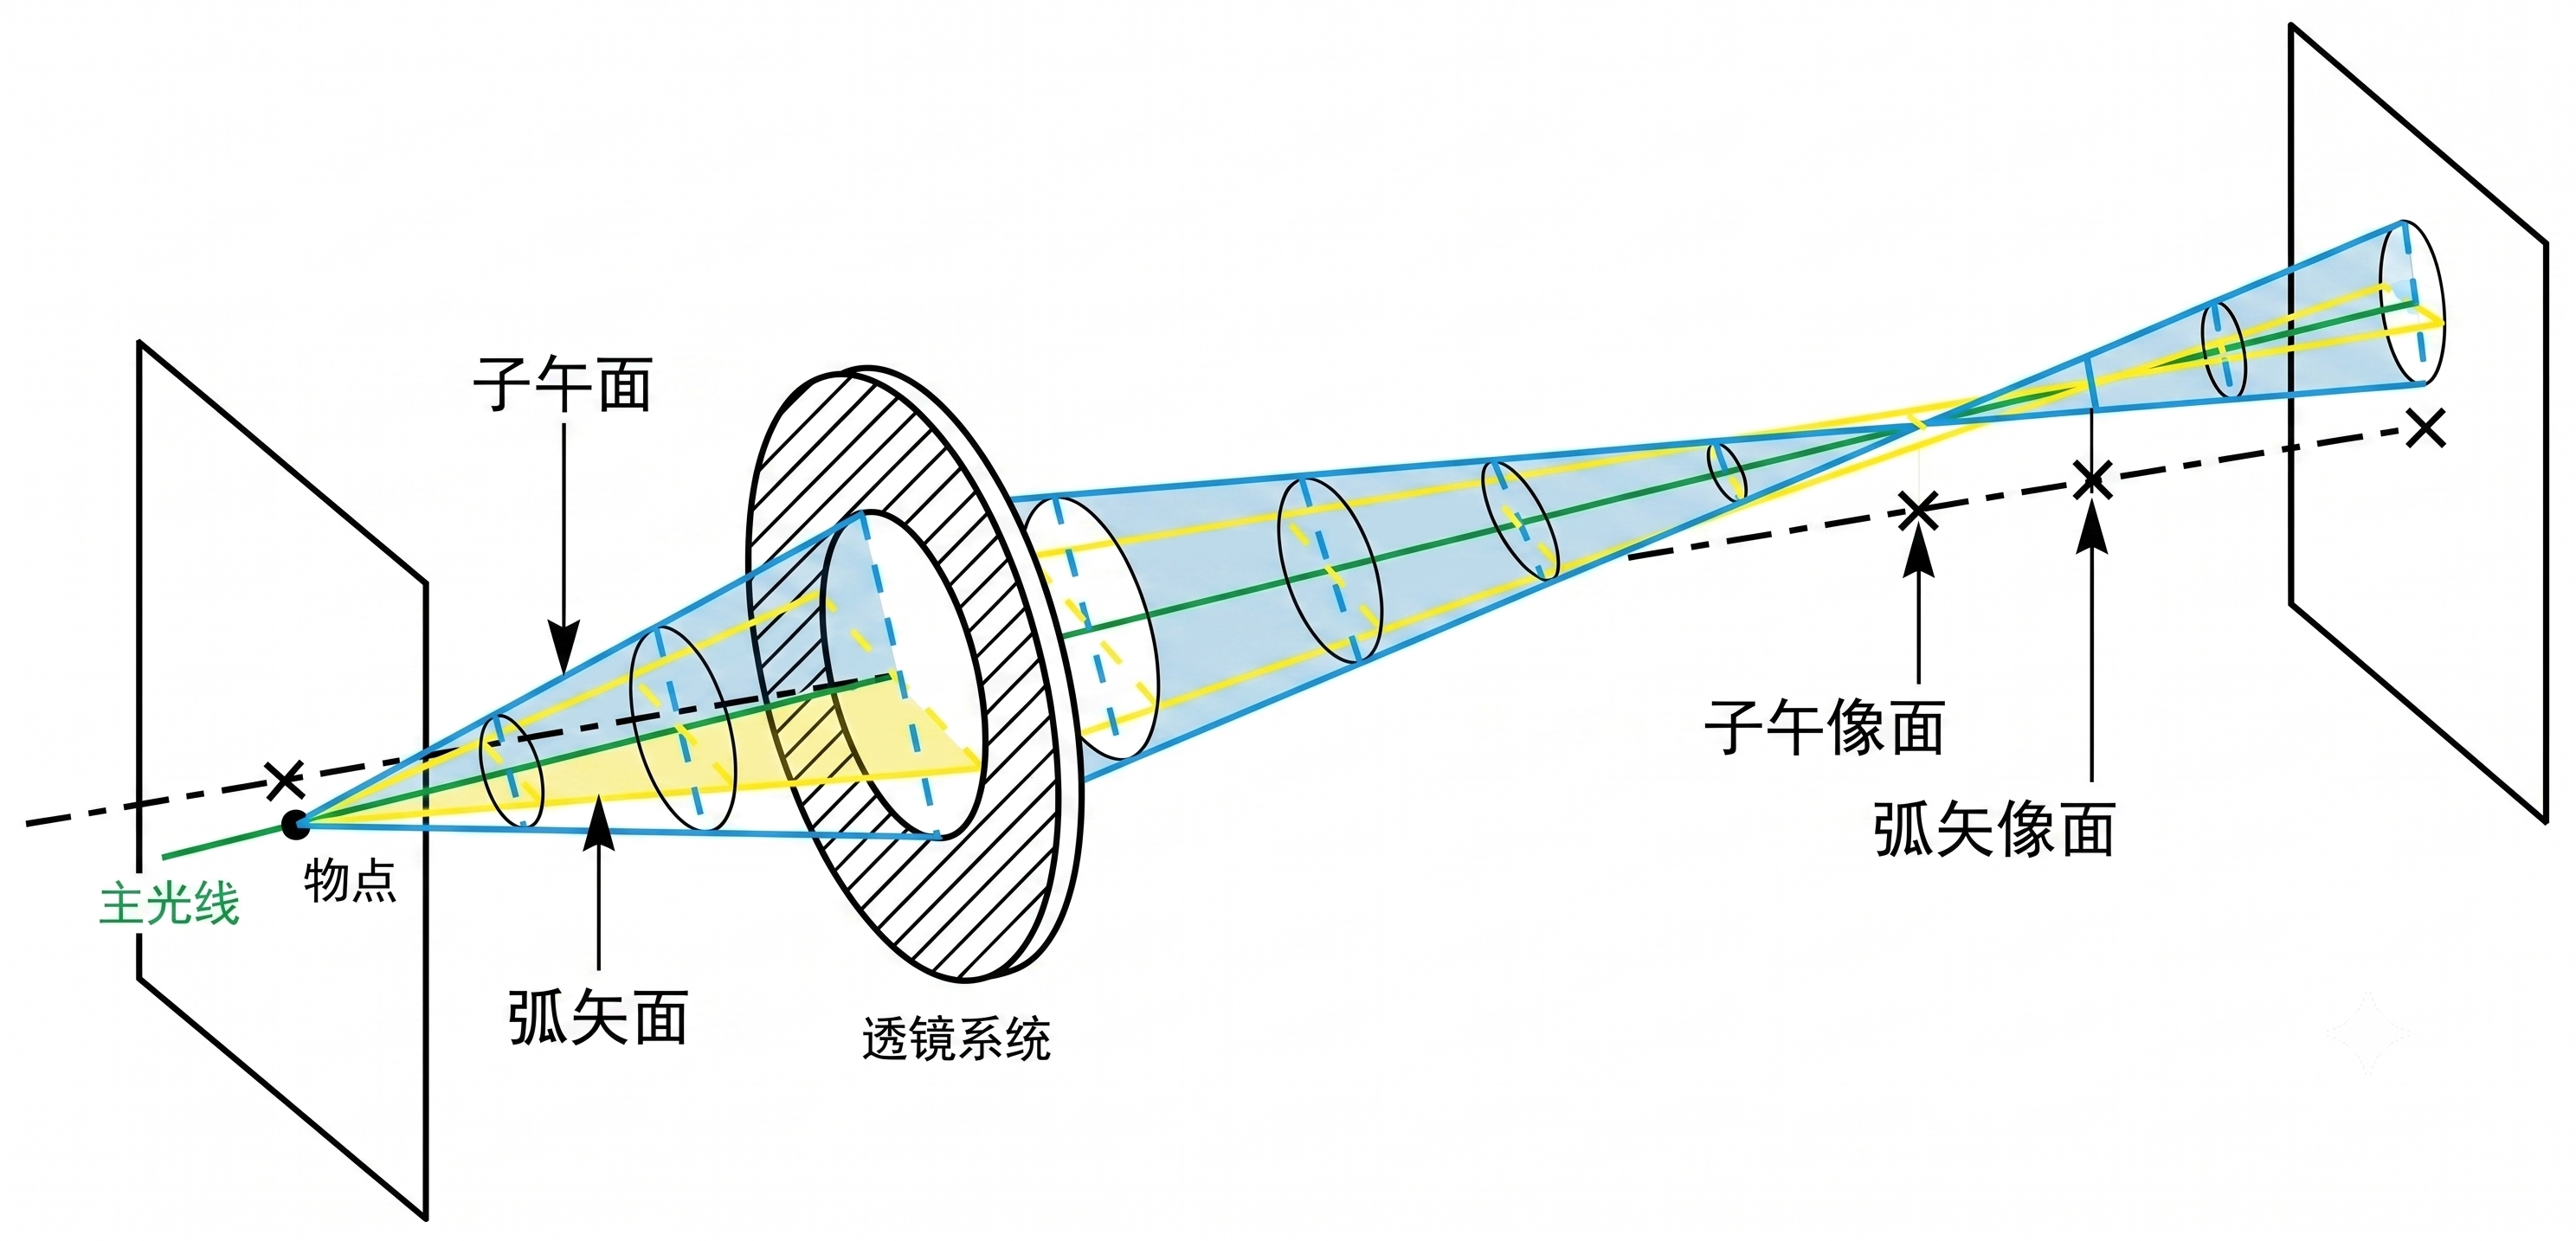
\includegraphics[width=\textwidth]{Figure/图片19.png}
                \caption{像散发生时的光路图}
                \label{fig:astigmatism_ray}
            \end{figure}
        \end{column}
        \hfill
        \begin{column}{.50\textwidth}
            \textbf{像散的本质：}
            \begin{itemize}
                \item 子午聚焦面上，弧矢光线尚未聚焦
                \item 弧矢聚焦面上，子午光线已开始发散
            \end{itemize}

            \textbf{像散矫正策略：}
            \begin{enumerate}
                \item \alert{改变光阑位置}：改变轴外光束入射对称性
                \item \alert{非球面透镜}：同时改变两方向光焦度分布
                \item \alert{对称光学结构}：前后对称自然抵消像散
            \end{enumerate}

            \alert{关键：}存在最佳光阑位置使像散为零。这与场曲不同——场曲与光阑位置无关。
        \end{column}
    \end{columns}
\end{frame}

\englishtitle{Distinguishing Three Types of Linear Aberrations}
\begin{frame}{三种线性像差的区分方法}
    \begin{figure}
        \centering
        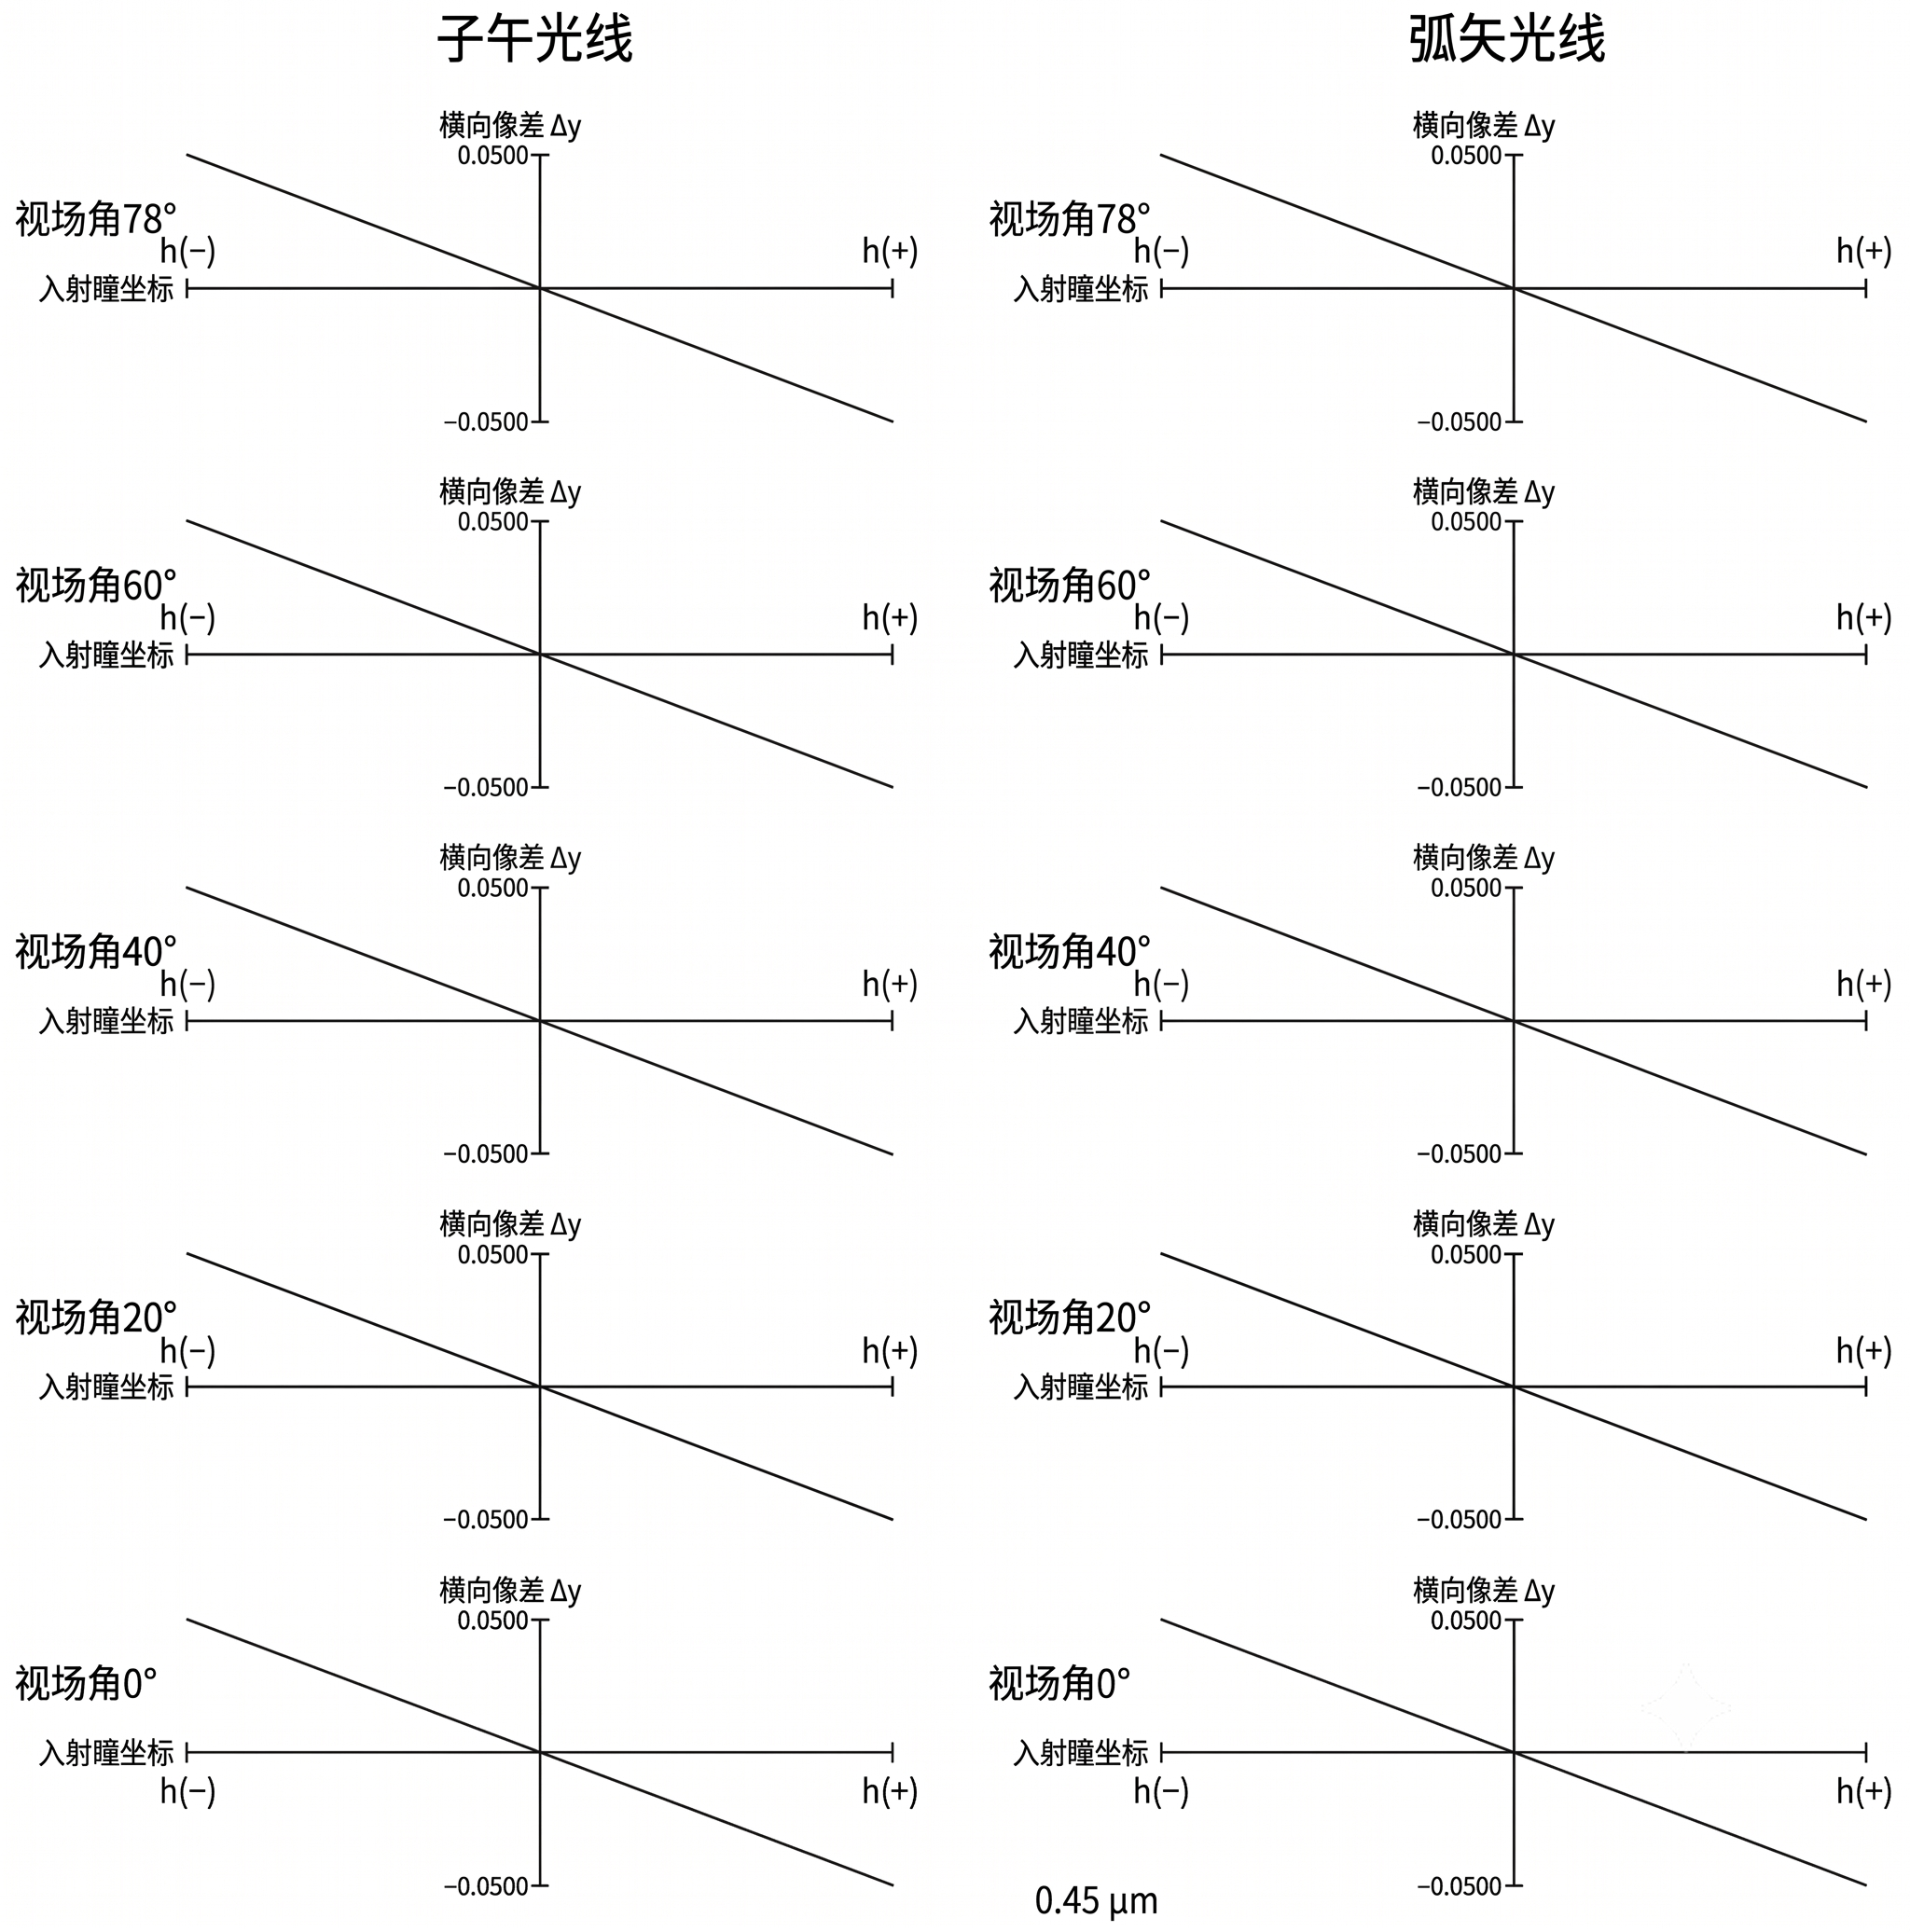
\includegraphics[width=0.3\textwidth]{Figure/图片20.png}\hfill
        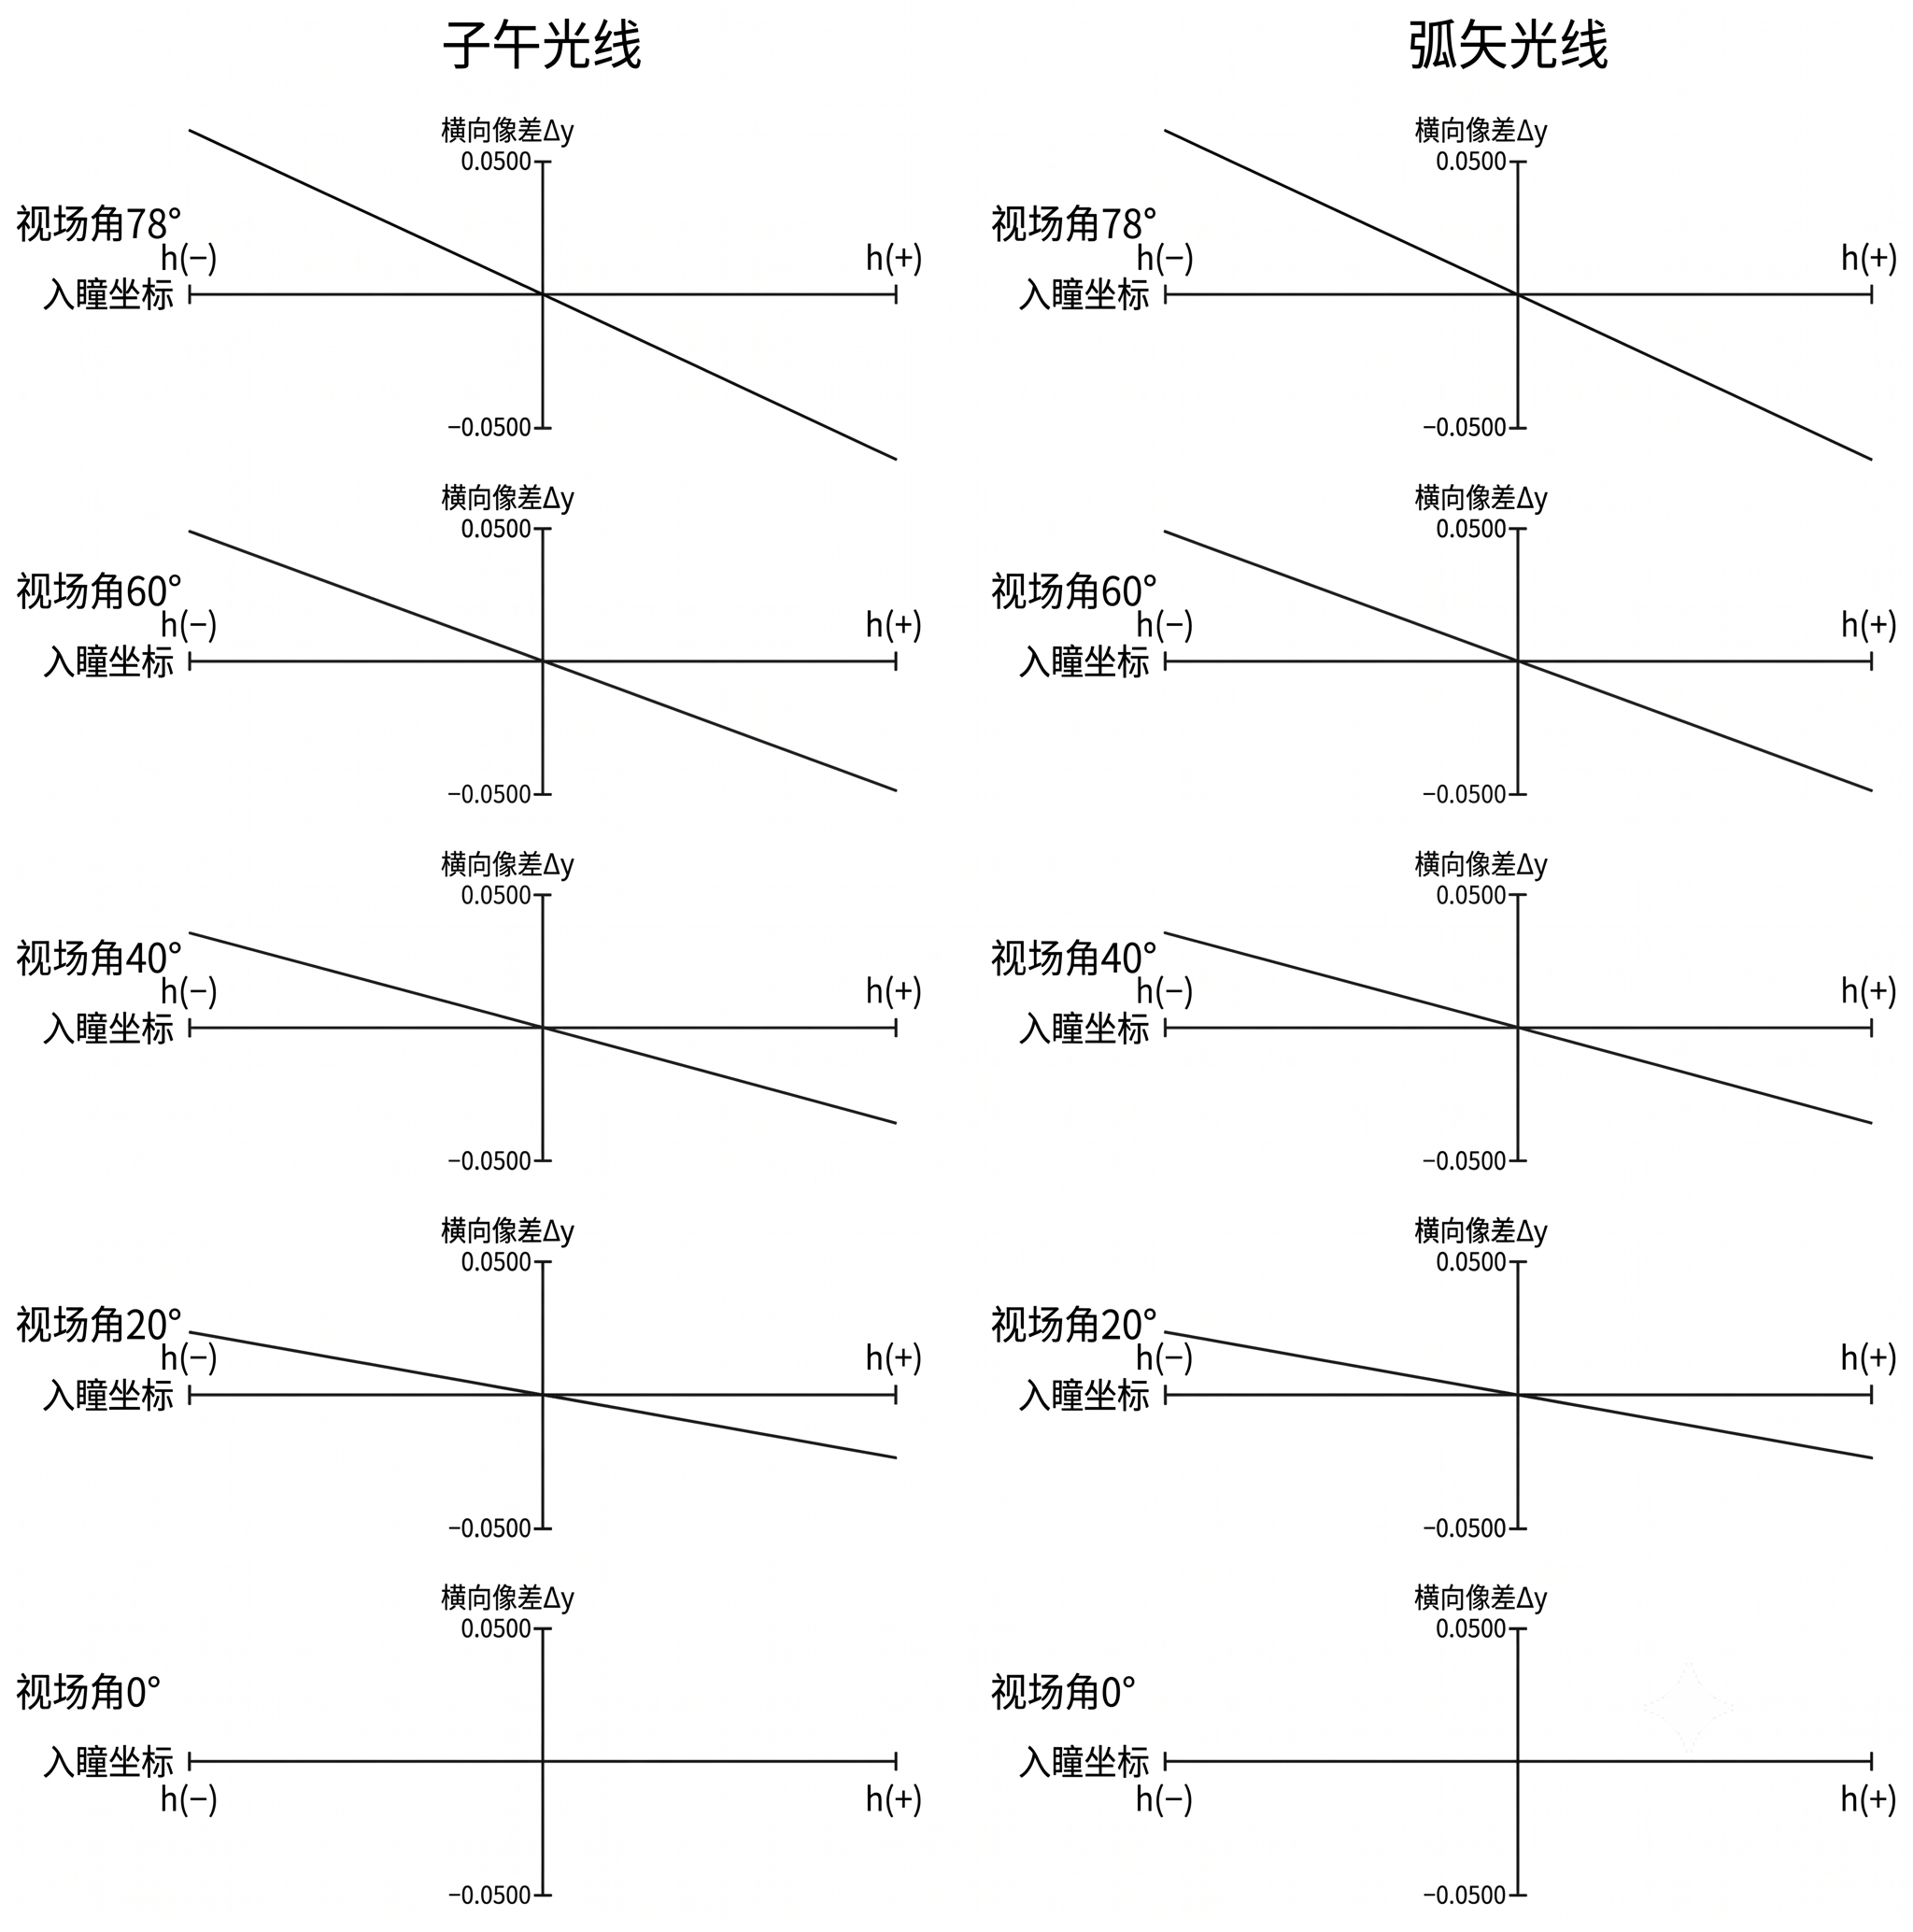
\includegraphics[width=0.3\textwidth]{Figure/图片21.png}\hfill
        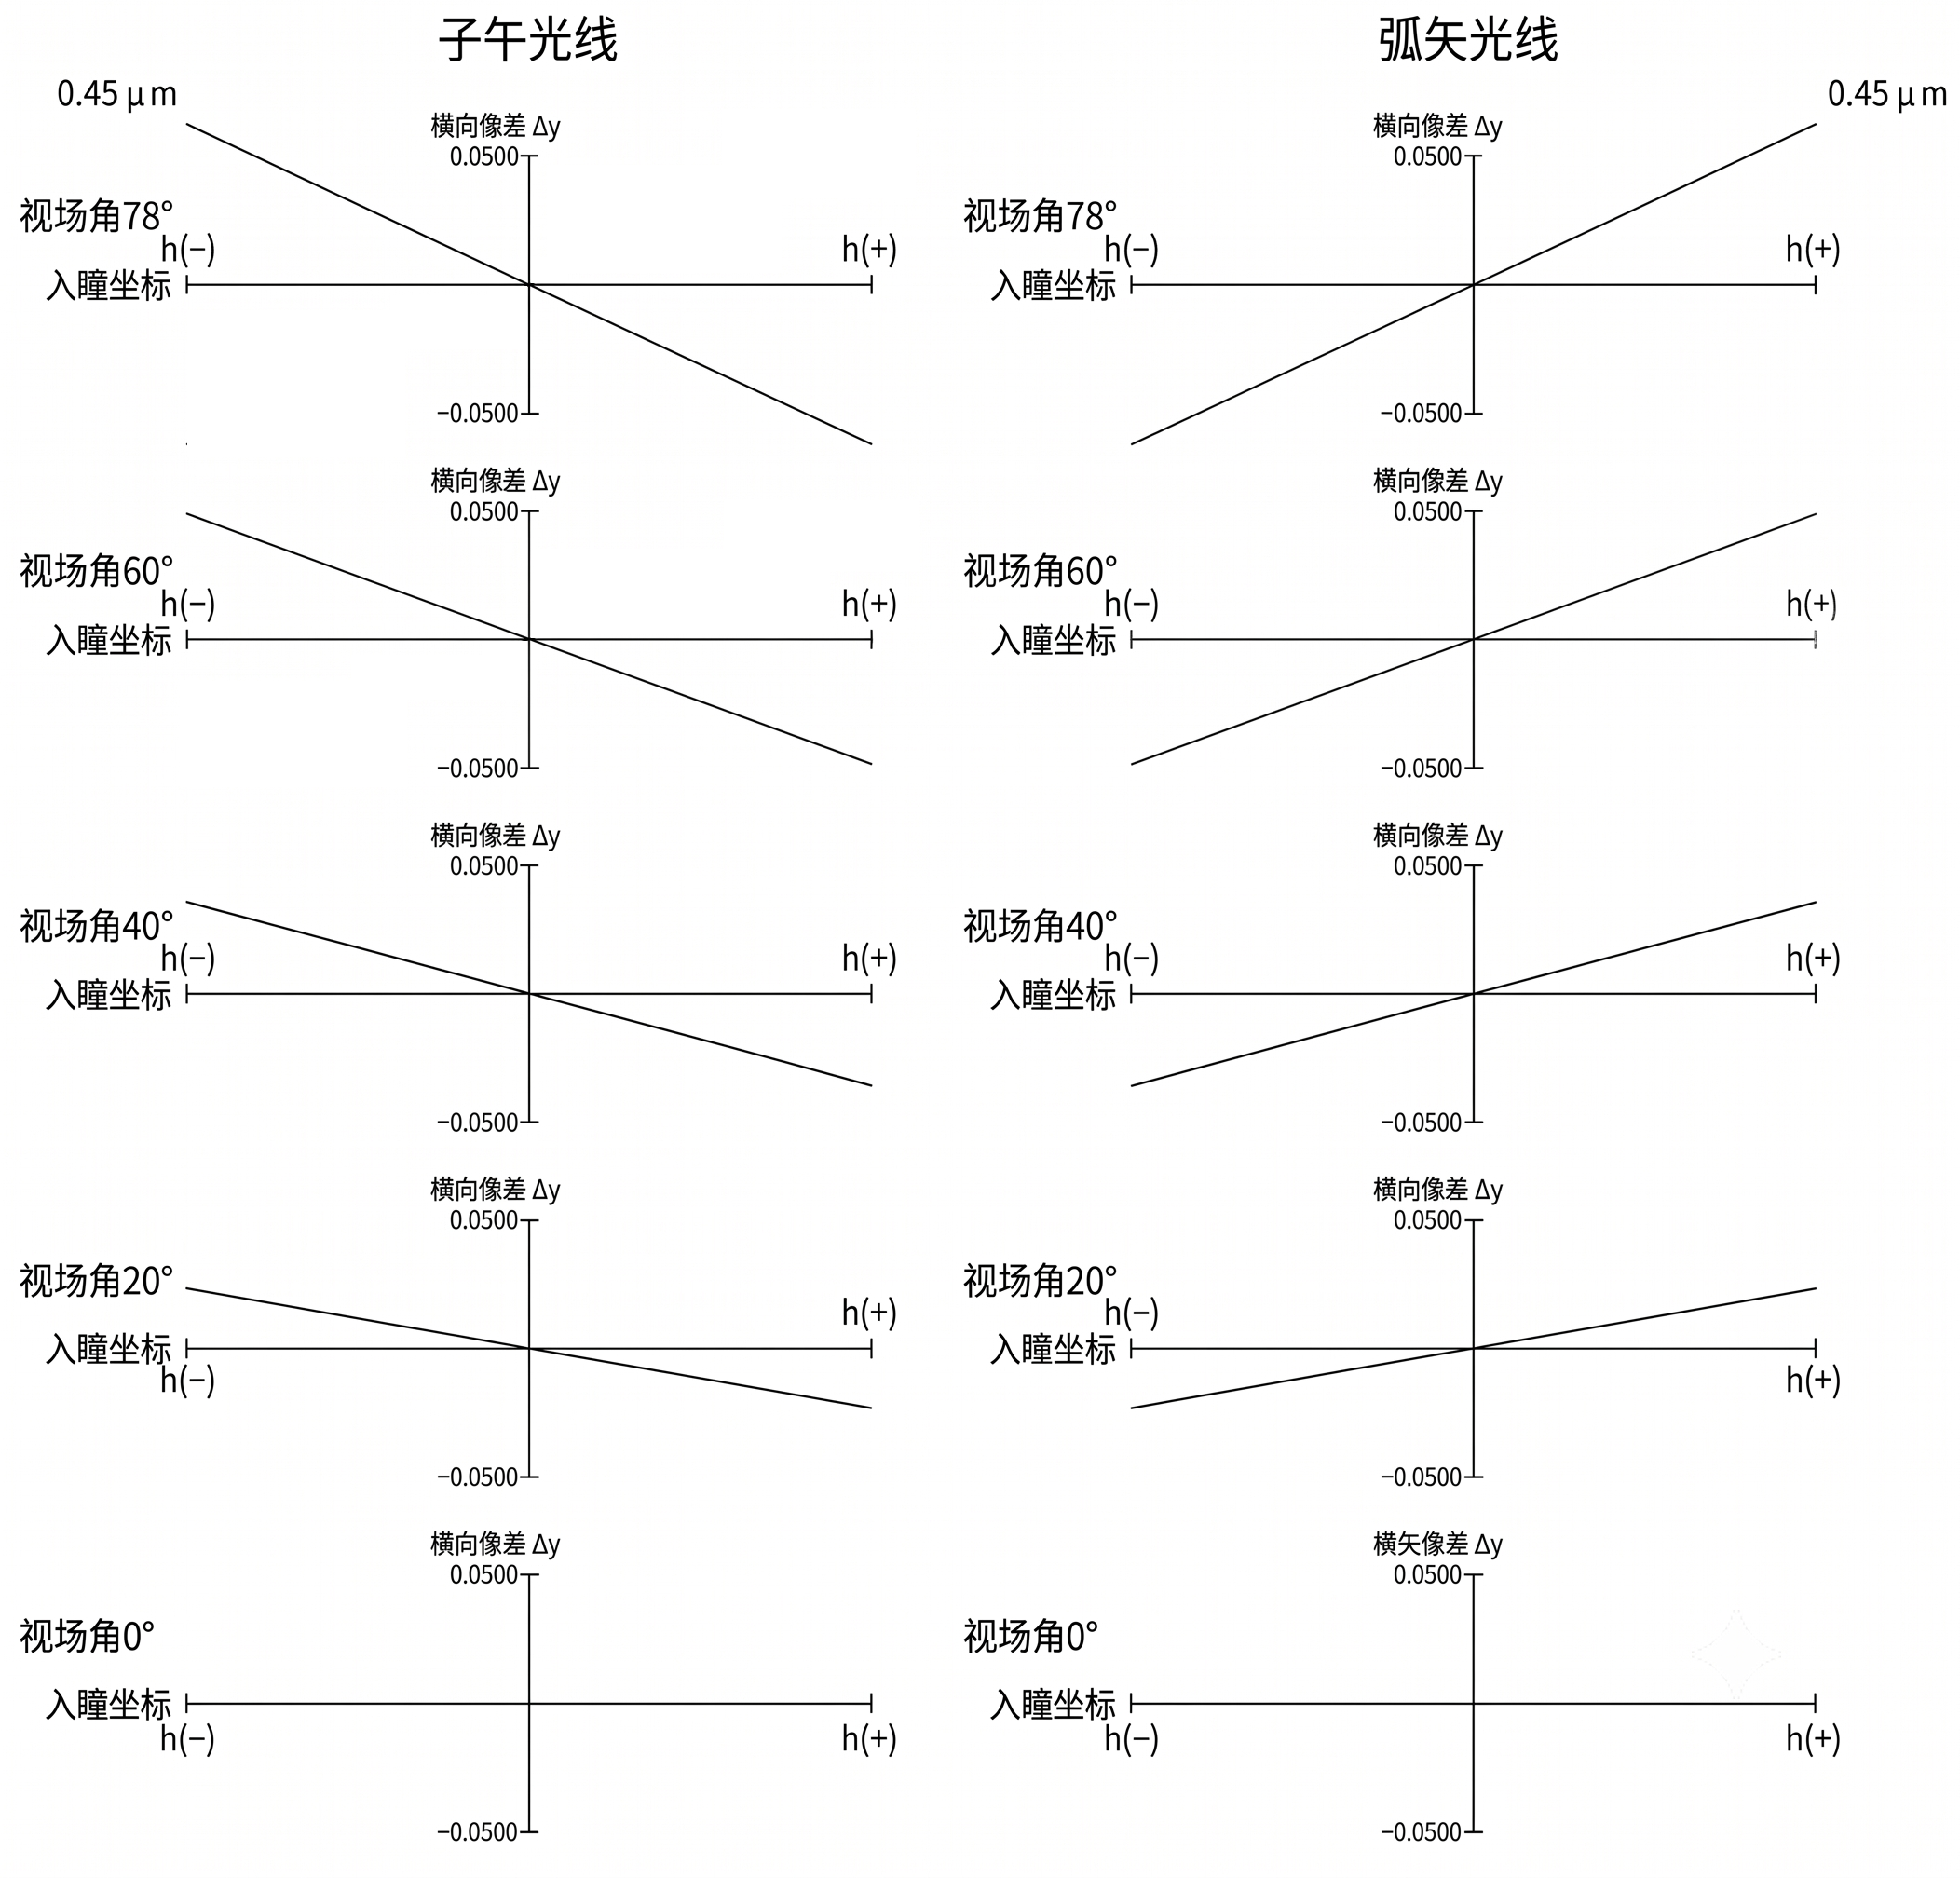
\includegraphics[width=0.3\textwidth]{Figure/图片22.png}
        \caption{离焦(左)：斜率均一\quad 场曲(中)：子午/弧矢一致\quad 像散(右)：子午/弧矢不同}
        \label{fig:linear_distinction}
    \end{figure}

    \smallbreak
    \begin{table}
        \centering
        \begin{tabular}{c|c|c}
            \toprule
            \textbf{像差类型} & \textbf{斜率与视场角关系} & \textbf{子午与弧矢关系} \\
            \midrule
            离焦 & 均一           & 一致 \\
            场曲 & 因视场角而异   & 一致 \\
            像散 & 因视场角而异   & \alert{不一致} \\
            \bottomrule
        \end{tabular}
        \caption{离焦、场曲与像散的区分准则}
        \label{tab:linear_aberration}
    \end{table}
\end{frame}

\subsection{色差、渐晕与衍射极限}

\englishtitle{Vignetting and Pupil Aberration}
\begin{frame}{渐晕与光瞳像差}
    \begin{columns}[T]
        \begin{column}{.45\textwidth}
            \begin{figure}
                \centering
                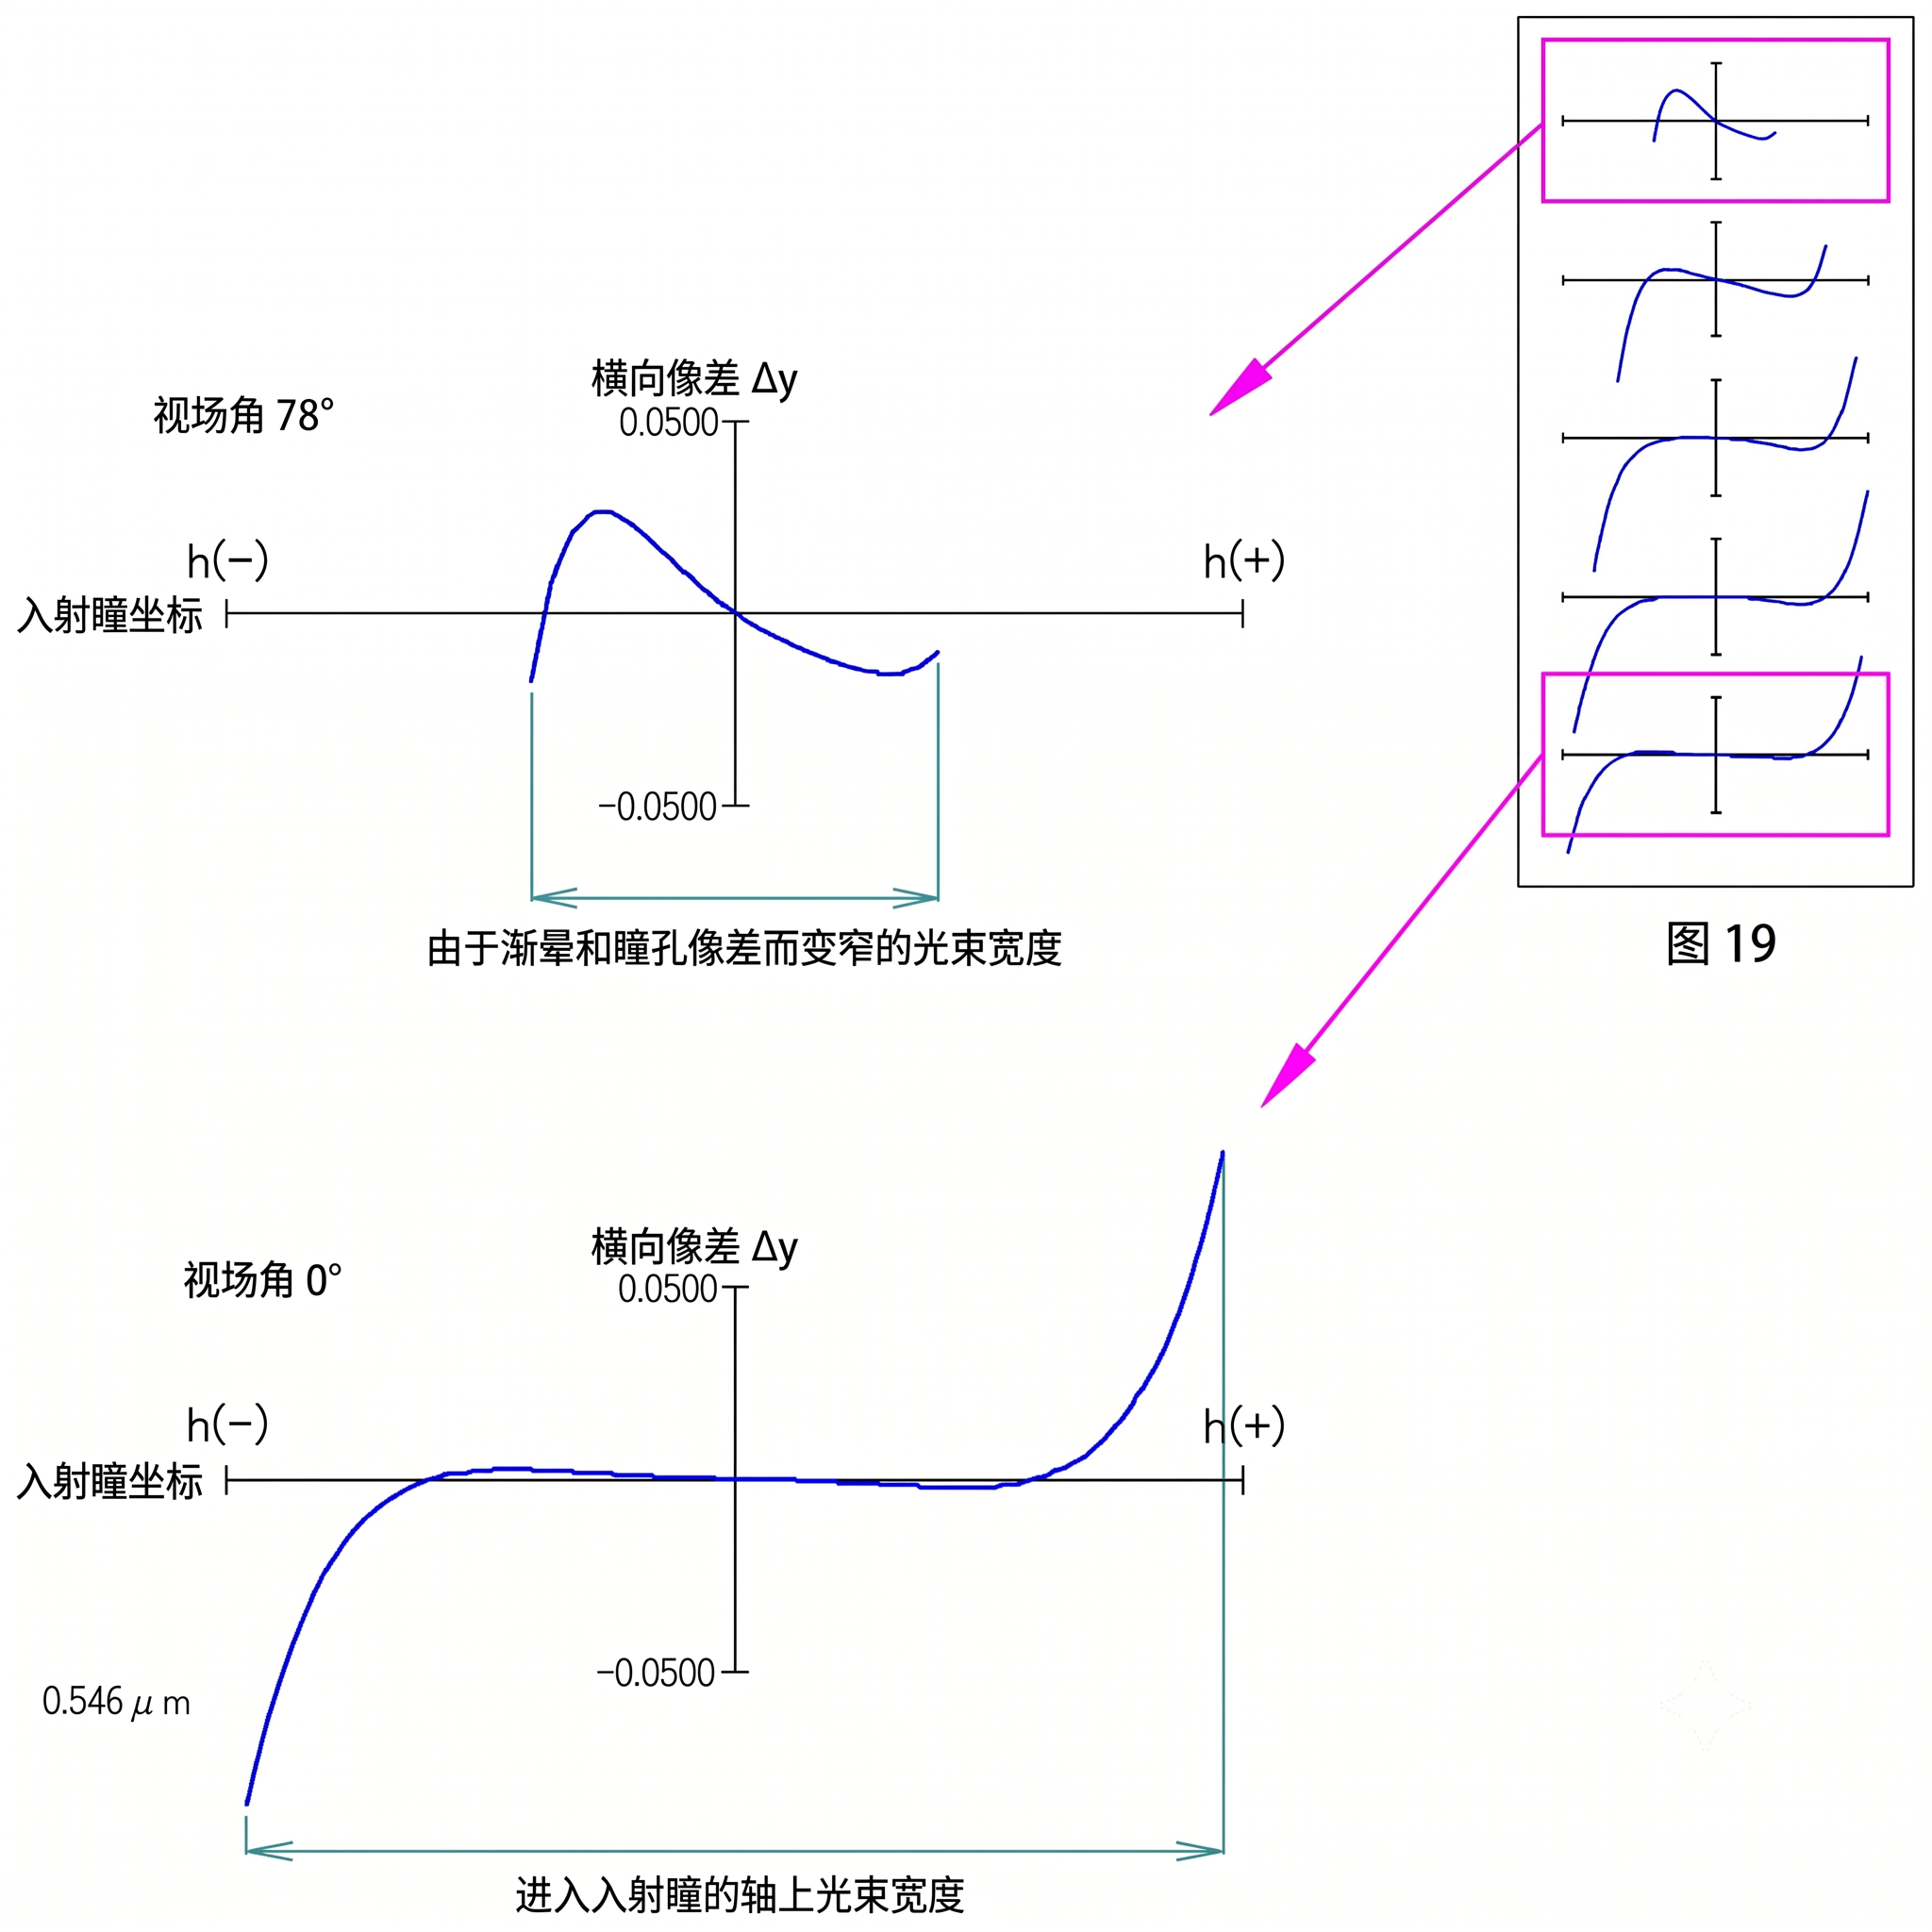
\includegraphics[width=0.9\textwidth]{Figure/图片27.png}
                \caption{渐晕和光瞳像差引起宽度差异}
                \label{fig:vignetting}
            \end{figure}
        \end{column}
        \hfill
        \begin{column}{.55\textwidth}
            比较 $0^\circ$ 和 $78^\circ$ 视场角的横向像差图，轴外光束宽度\alert{更窄}。

            \bigbreak
            \begin{itemize}
                \item \alert{渐晕(Vignetting)}：大视场下镜筒或透镜边缘遮挡光束
                \item \alert{光瞳像差}：轴上与轴外光束形成的入瞳形状不同
            \end{itemize}

            \textbf{判断方法：}比较满刻度(近轴入瞳直径)与实际宽度。
            \alert{注意：}入瞳直径是近轴量，不受渐晕影响。
        \end{column}
    \end{columns}
\end{frame}

\englishtitle{Axial Chromatic Aberration}
\begin{frame}{轴向色差}
    \begin{columns}[T]
        \begin{column}{.46\textwidth}
            \begin{figure}
                \centering
                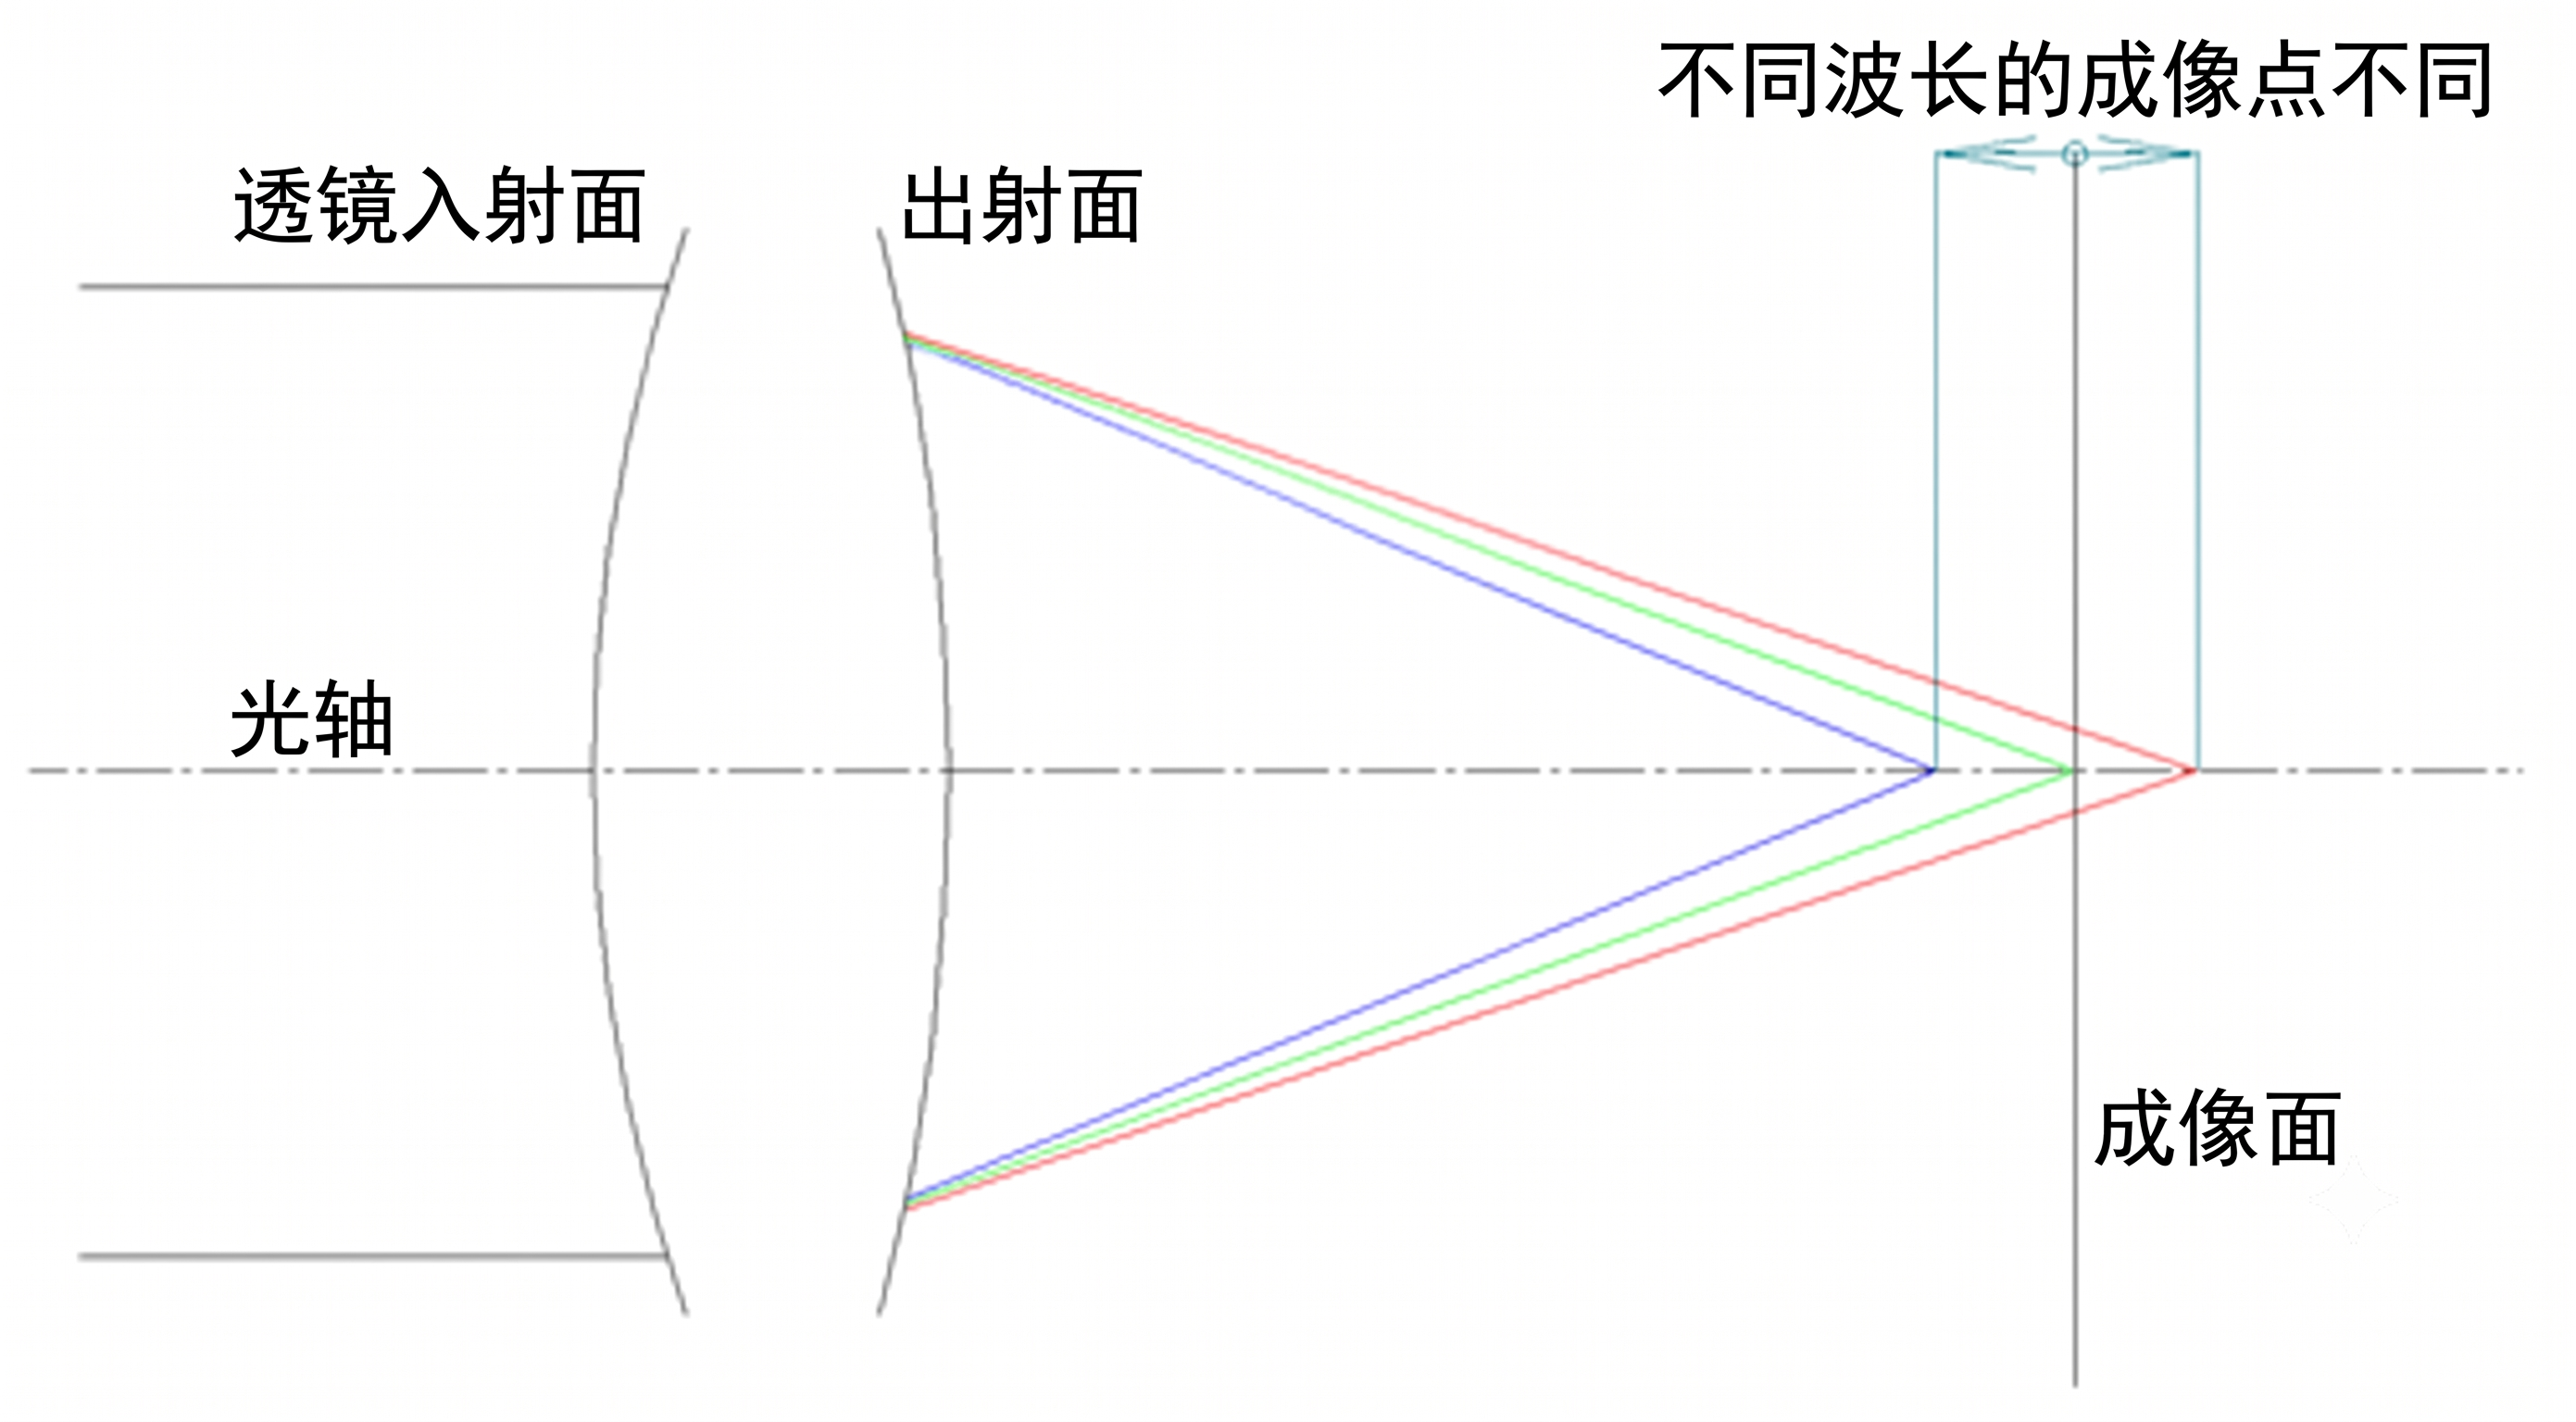
\includegraphics[width=0.98\textwidth]{Figure/图片30.png}\\[3pt]
                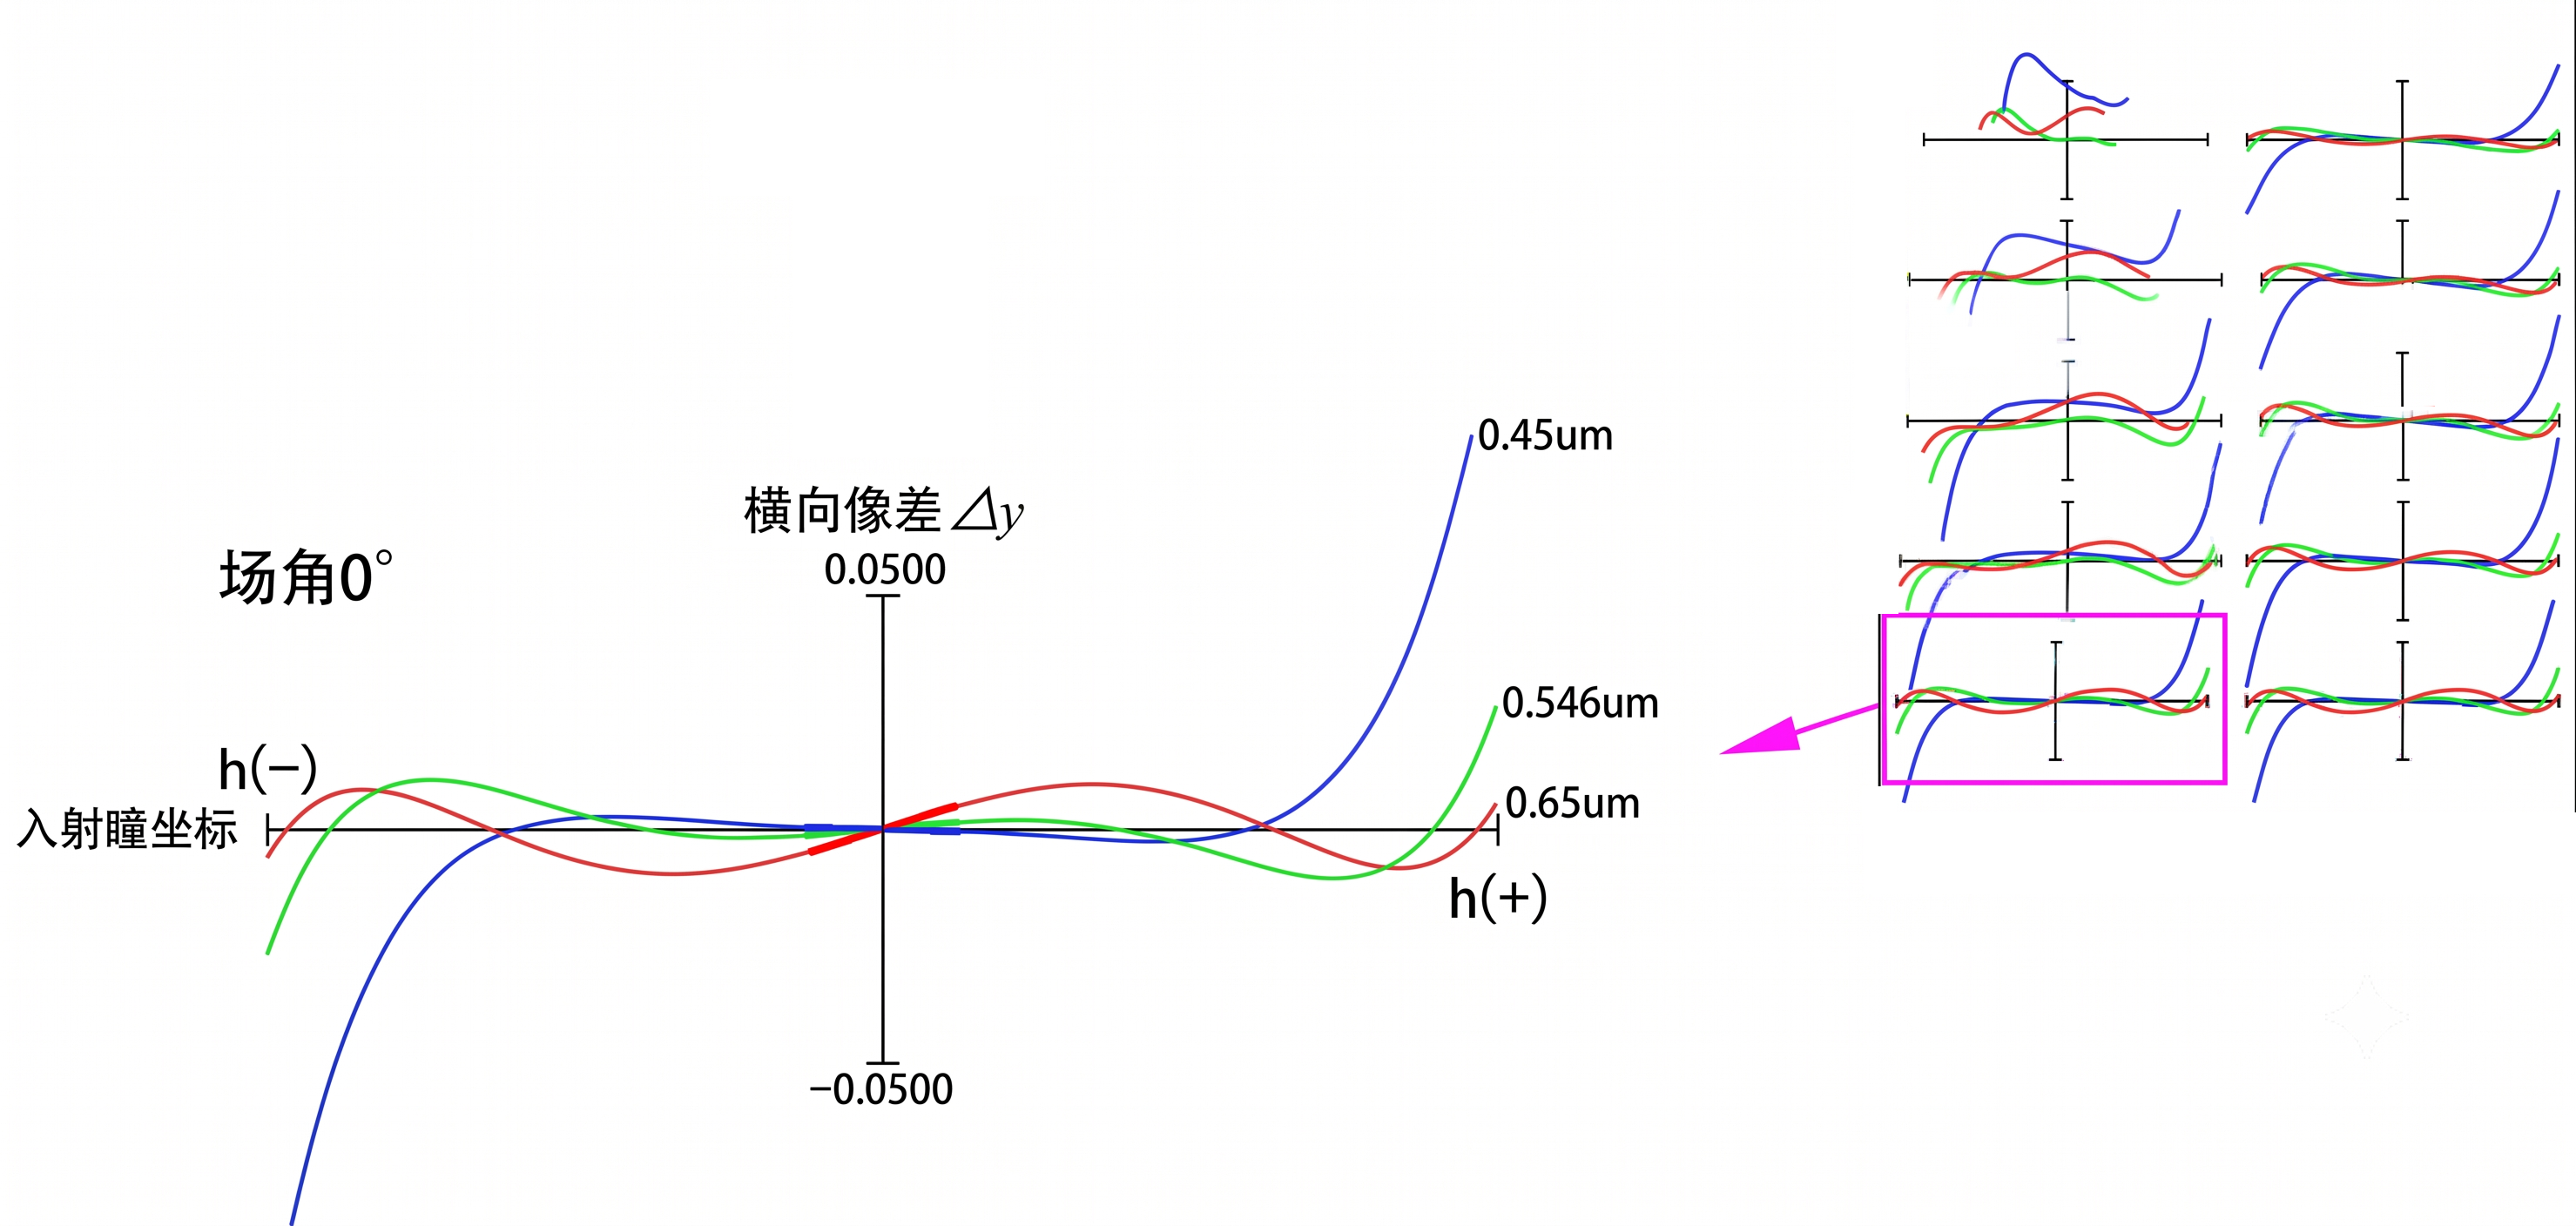
\includegraphics[width=0.98\textwidth]{Figure/图片28.png}
                \caption{轴向色差的光路示意与横向像差图特征}
                \label{fig:axial_color}
            \end{figure}
        \end{column}
        \hfill
        \begin{column}{.54\textwidth}
            \textbf{轴向色差(纵色差/位置色差)：}
            \bigbreak
            轴上光束横向像差图\alert{原点附近}斜率因波长不同——近轴像点位置具有\alert{波长依赖性}。

            \bigbreak
            \textbf{物理机制：}
            \begin{itemize}
                \item $n(\lambda)$ 随波长变化：短波折射率高，焦点近
                \item 原点附近球差($\propto h^3$)和彗差($\propto h^2$)影响最小
                \item 轴向色差($\propto h^1$)在原点附近\alert{占主导}
            \end{itemize}

            矫正：\alert{消色差双透镜(achromat)}。
        \end{column}
    \end{columns}
\end{frame}

\englishtitle{Lateral Chromatic Aberration}
\begin{frame}{倍率色差}
    \begin{columns}[T]
        \begin{column}{.46\textwidth}
            \begin{figure}
                \centering
                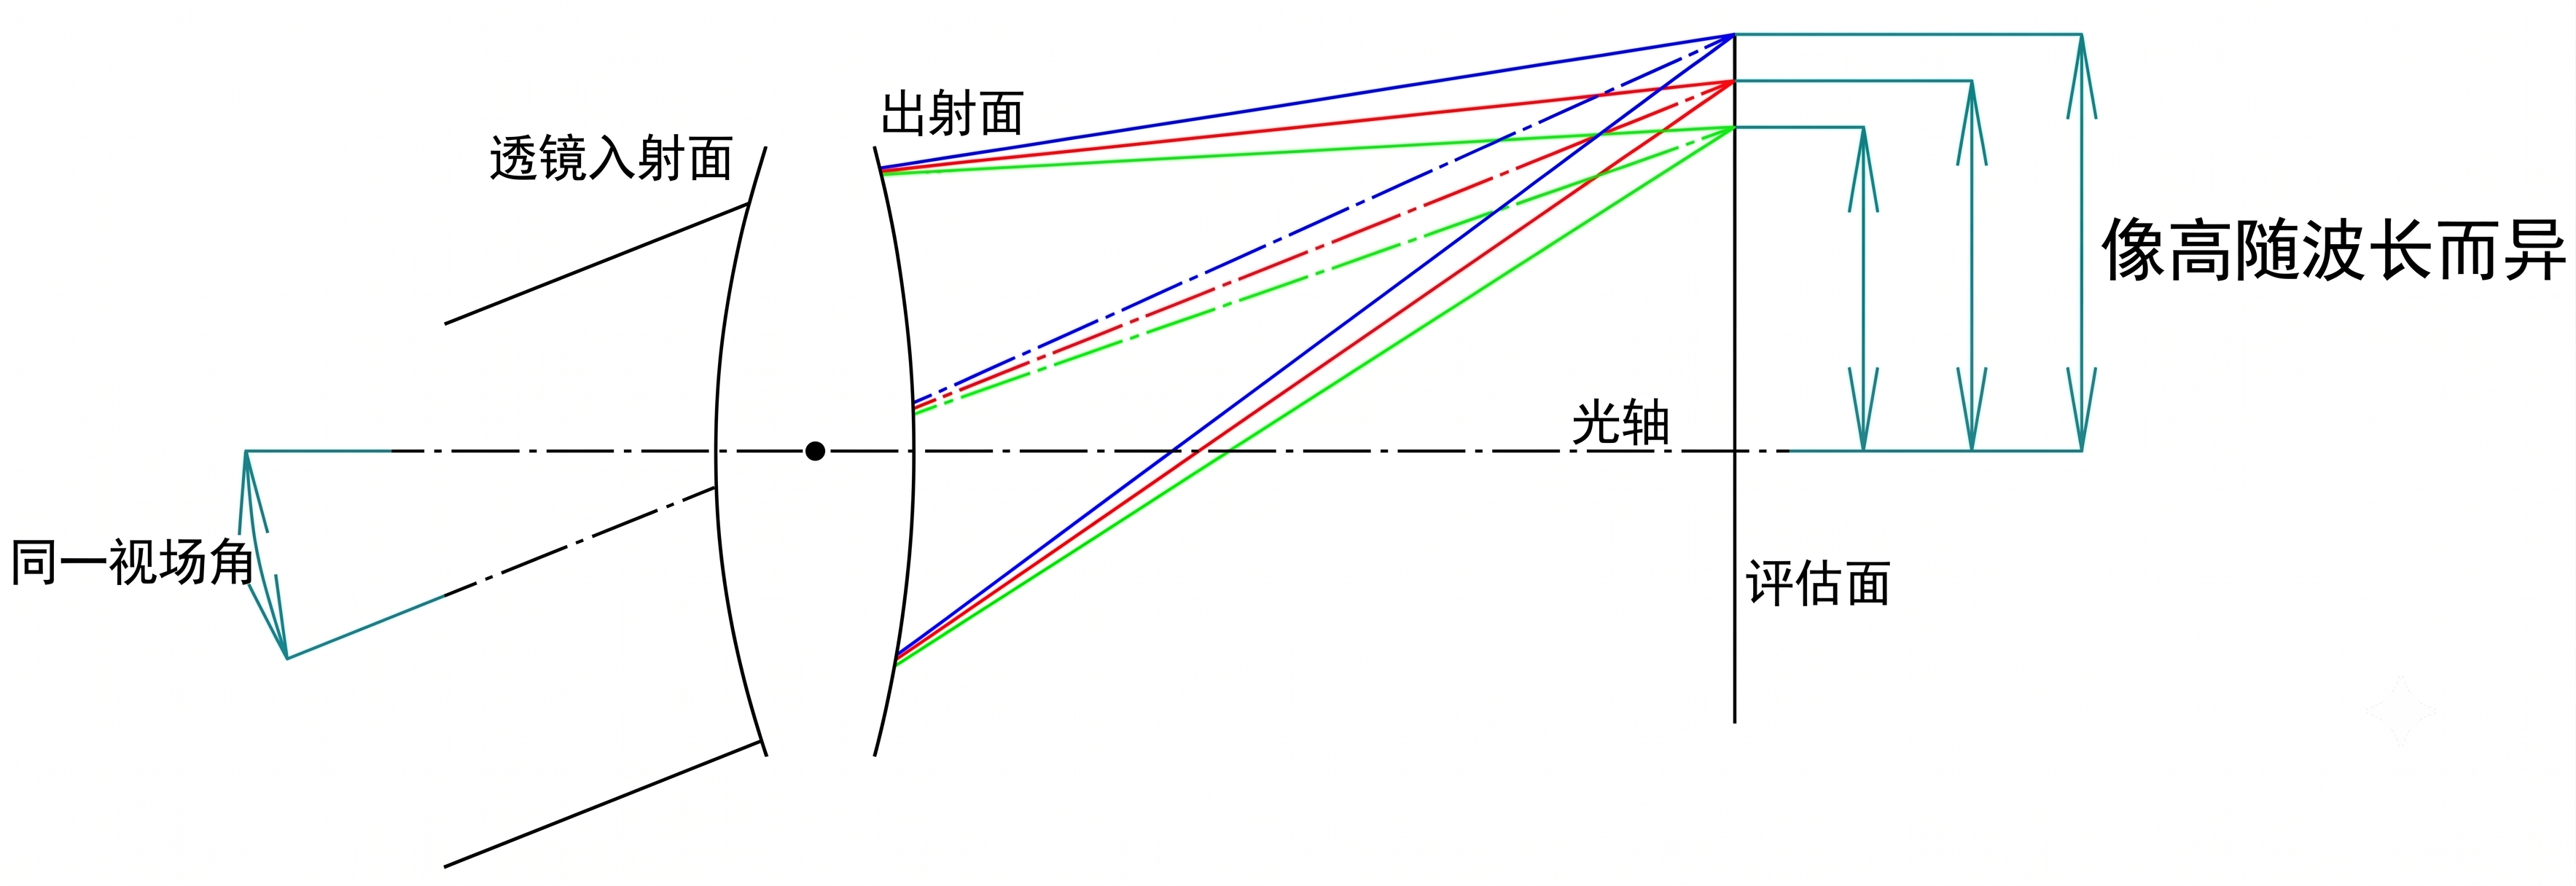
\includegraphics[width=0.98\textwidth]{Figure/图片31.png}\\[3pt]
                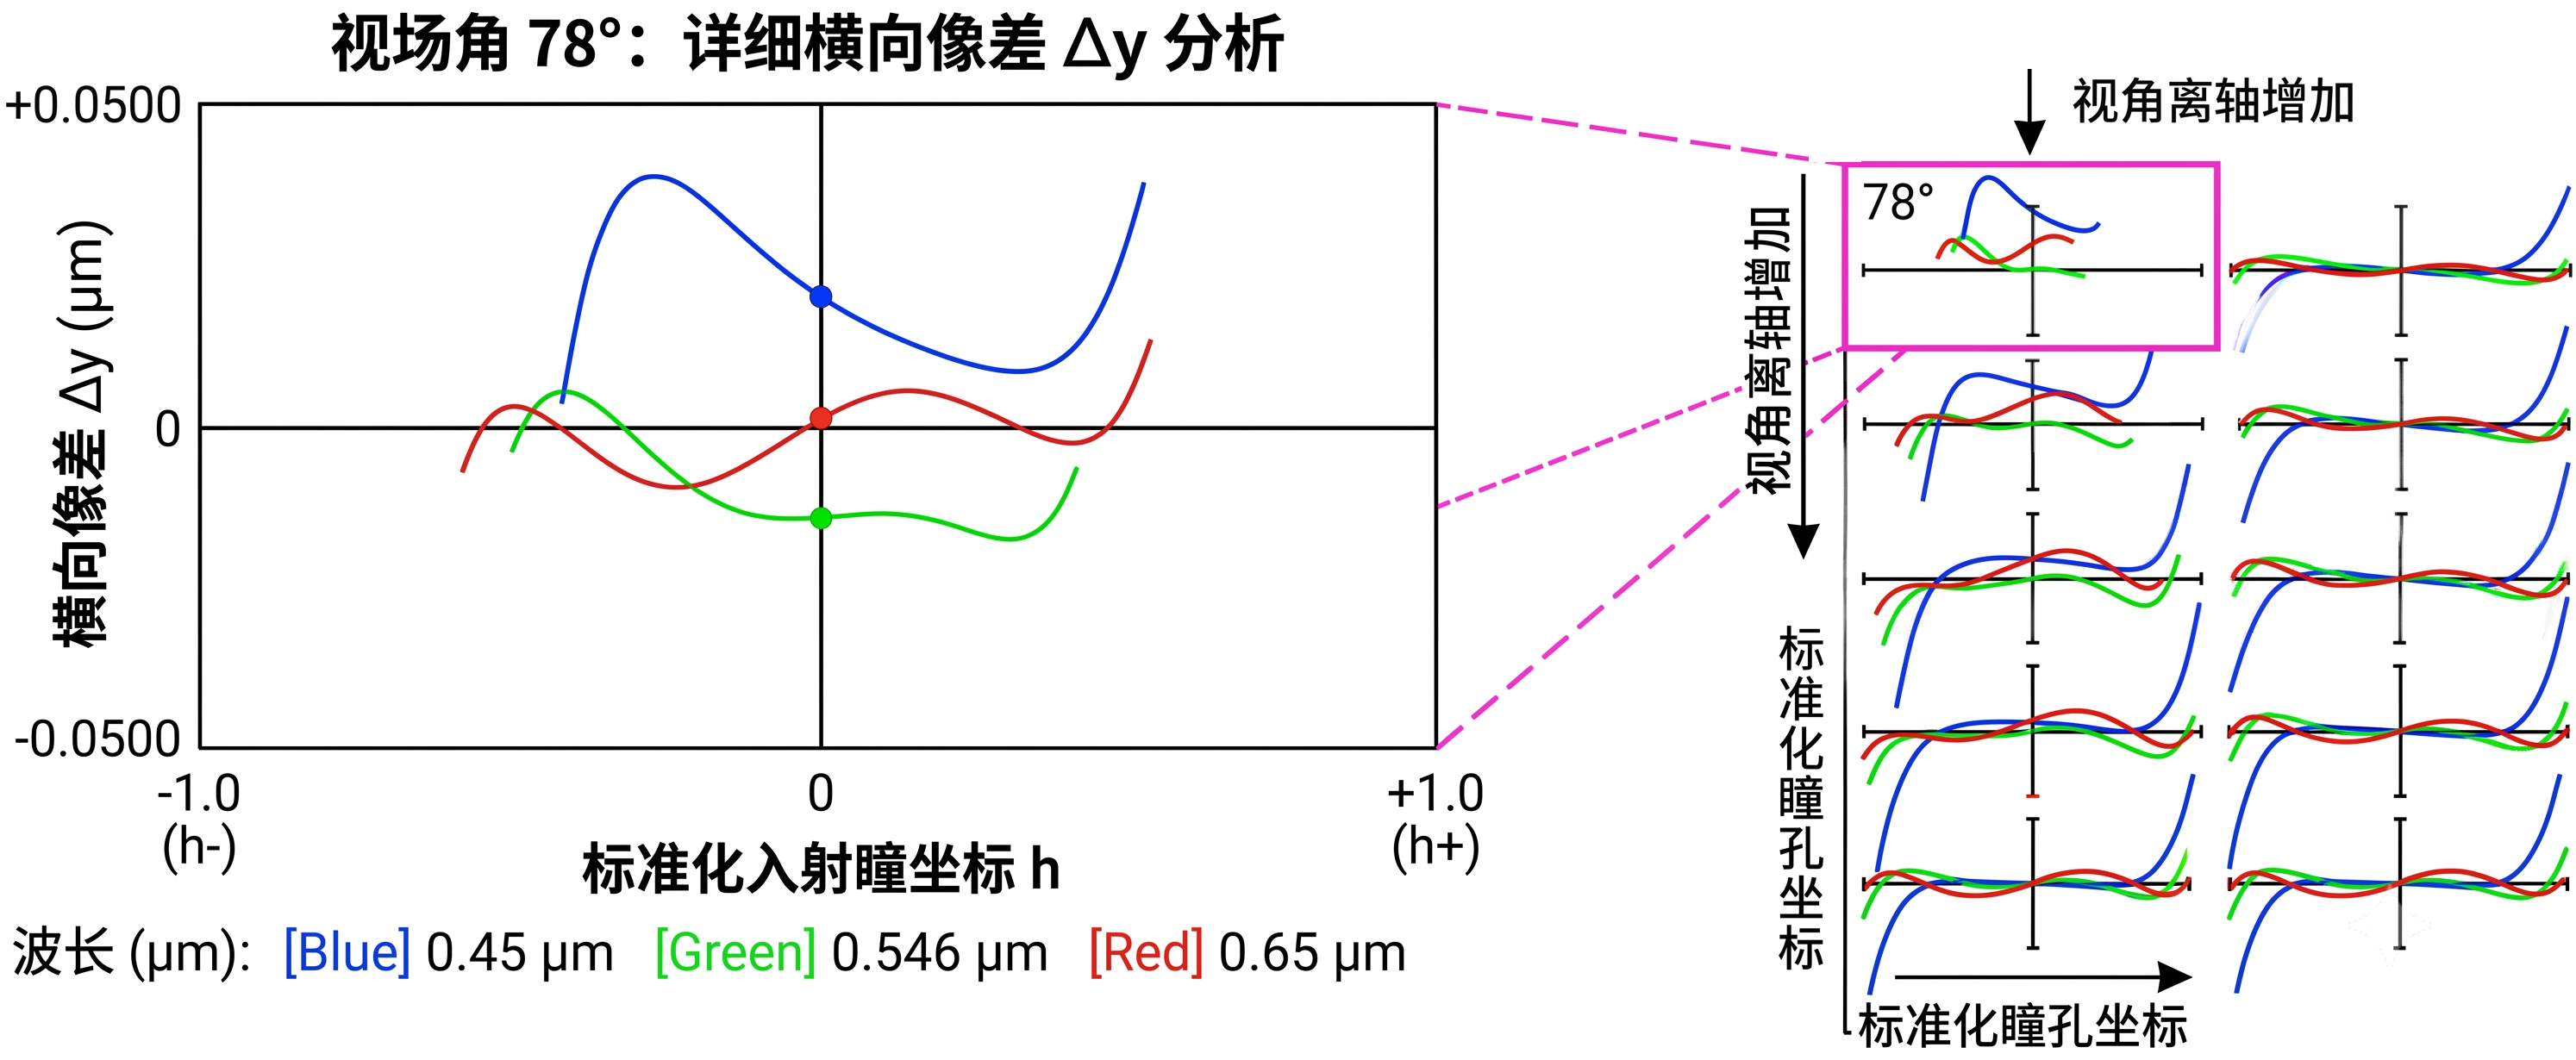
\includegraphics[width=0.98\textwidth]{Figure/图片29.png}
                \caption{倍率色差的光路示意与横向像差图特征}
                \label{fig:lateral_color}
            \end{figure}
        \end{column}
        \hfill
        \begin{column}{.54\textwidth}
            \textbf{倍率色差(横向色差)：}
            \bigbreak
            轴外光束横向像差图与\alert{纵轴交点坐标}因波长不同——不同波长主光线在像面上距光轴\alert{不同高度}成像。

            \bigbreak
            \begin{itemize}
                \item 不同波长以不同倍率成像
                \item 即使轴向色差被完全校正，倍率色差仍可能存在
                \item 在像面\alert{边缘}最为显著
            \end{itemize}

            矫正：\alert{对称光学结构}。
        \end{column}
    \end{columns}
\end{frame}

\englishtitle{Systematic Comparison of Two Chromatic Aberrations}
\begin{frame}{两种色差的系统对比}
    \begin{table}
        \centering
        \small
        \begin{tabular}{p{2.2cm}|p{4.2cm}|p{4.2cm}}
            \toprule
            \textbf{特征} & \textbf{轴向色差} & \textbf{倍率色差} \\
            \midrule
            别名 & 纵色差、位置色差 & 横向色差、放大率色差 \\
            观察位置 & 轴上光束、原点斜率 & 轴外光束、纵轴交点 \\
            像差图表现 & 近轴斜率随波长变化 & 纵轴截距随波长变化 \\
            物理含义 & 焦点位置不同 & 放大率不同 \\
            光束类型 & $0^\circ$ 视场角 & 有视场角 \\
            校正方式 & 消色差双透镜 & 对称光学结构 \\
            \bottomrule
        \end{tabular}
        \caption{轴向色差与倍率色差的全面对比}
        \label{tab:chromatic_compare}
    \end{table}
\end{frame}

\englishtitle{Abbe Number and Dispersion of Optical Glass}
\begin{frame}{阿贝数与光学玻璃的色散特性}
    \begin{columns}[T]
        \begin{column}{.50\textwidth}
            \begin{figure}
                \centering
                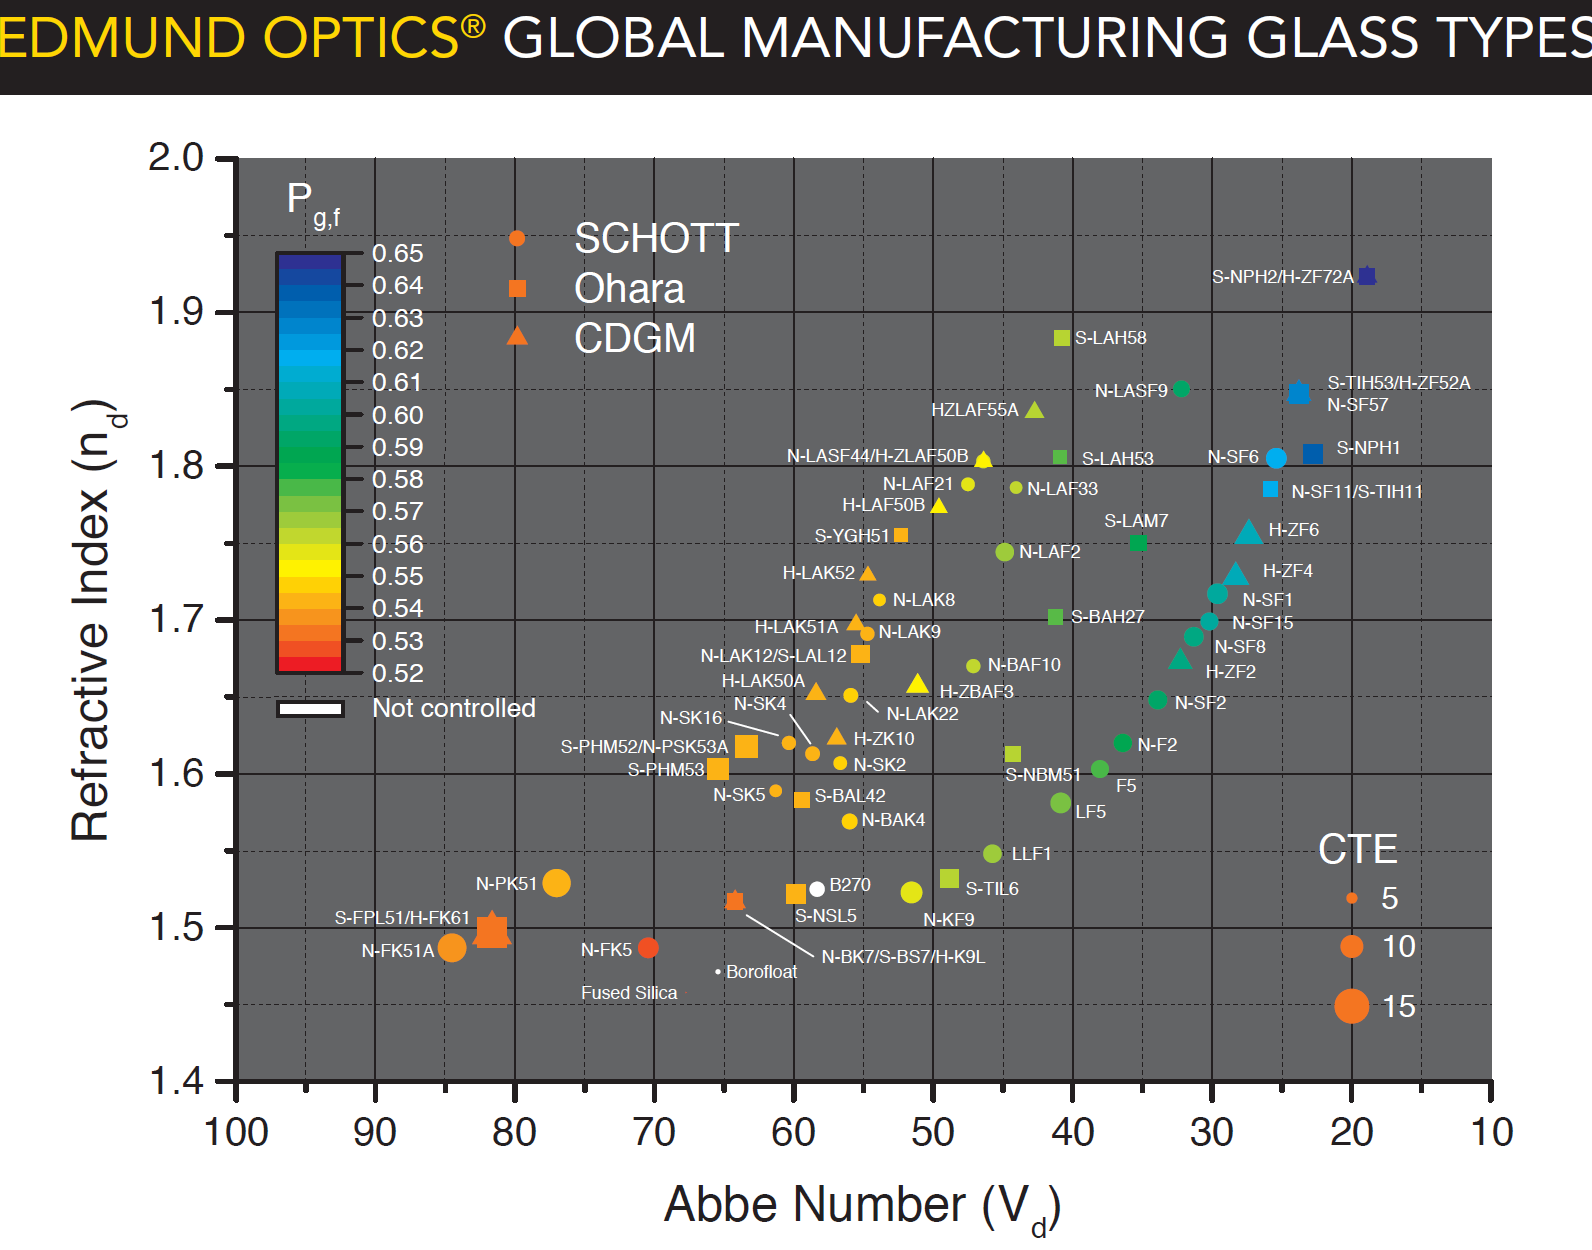
\includegraphics[width=0.95\textwidth]{Figure/Abbe.png}
                \caption{常见光学玻璃的阿贝图——折射率 $n_d$ 与阿贝数 $\nu_d$}
                \label{fig:abbe}
            \end{figure}
        \end{column}
        \hfill
        \begin{column}{.50\textwidth}
            \textbf{阿贝数(Abbe Number)：}
            \begin{equation}
                \nu_d = \frac{n_d - 1}{n_F - n_C}
                \label{eq:abbe}
            \end{equation}
            其中 $n_d$, $n_F$, $n_C$ 分别为 d, F, C 谱线的折射率。

            \bigbreak
            \begin{itemize}
                \item \alert{低阿贝数($\nu_d < 50$)}：高色散(火石玻璃 F 系列)
                \item \alert{高阿贝数($\nu_d > 55$)}：低色散(冕牌玻璃 K 系列)
                \item 消色差设计：搭配高/低阿贝数玻璃，如 BK7+F2
            \end{itemize}
        \end{column}
    \end{columns}
\end{frame}

\englishtitle{Diffraction Limit and Strehl Ratio}
\begin{frame}{衍射极限与斯特列尔比}
    \begin{columns}[T]
        \begin{column}{.60\textwidth}
            \textbf{衍射极限(Diffraction Limit)：}
            即使 $OPD = 0$，受孔径衍射效应限制，点像仍是\alert{艾里斑(Airy Disk)}。

            \bigbreak
            \textbf{斯特列尔比(Strehl Ratio, S.R.)：}
            \begin{equation}
                S.R. \approx \exp\!\left[-\left(\frac{2\pi}{\lambda}\,OPD_{\text{rms}}\right)^2\right]
                \label{eq:strehl}
            \end{equation}

            当像差较小时，可退化为\alert{马瑞夏近似}：
            \begin{equation}
                S.R. \approx 1 - \left(\frac{2\pi}{\lambda}\right)^2 (OPD_{\text{rms}})^2
                \label{eq:marechal}
            \end{equation}
        \end{column}
        \hfill
        \begin{column}{.40\textwidth}
            \begin{block}{瑞利判据}
                当 $|OPD_{\text{PV}}| \le \frac{\lambda}{4}$ 时，
                \alert{$S.R. > 0.8$}，系统达到\alert{衍射极限}。
            \end{block}

            \begin{table}
                \small
                \begin{tabular}{c|c|c}
                    \toprule
                    \textbf{OPD\textsubscript{PV}} & \textbf{S.R.} & \textbf{评价} \\
                    \midrule
                    $<\lambda/4$  & $>0.8$  & 衍射极限 \\
                    $\lambda/4\sim\lambda/2$ & $0.4\sim0.8$ & 可接受 \\
                    $>\lambda/2$ & $<0.4$   & 需矫正 \\
                    \bottomrule
                \end{tabular}
                \caption{像质评估对照}
                \label{tab:strehl_table}
            \end{table}
        \end{column}
    \end{columns}
\end{frame}

\englishtitle{Common Image-Quality Metrics in Optical Design}
\begin{frame}{光学设计中的常用像质评价量}
    \begin{columns}[T]
        \begin{column}{.52\textwidth}
            \begin{block}{几何光学评价}
                \begin{itemize}
                    \item \textbf{横向像差图 / Ray Fan}：最快定位球差、彗差、像散和色差来源
                    \item \textbf{点列图(Spot Diagram)}：观察能量在几何像点附近的扩散范围
                \end{itemize}
            \end{block}

            \begin{block}{波前评价}
                \begin{itemize}
                    \item \textbf{OPD / Wavefront Map}：直接关联瑞利判据和 Strehl 比
                    \item \textbf{PV / RMS}：适合做容差和优化目标的量化指标
                \end{itemize}
            \end{block}
        \end{column}
        \hfill
        \begin{column}{.48\textwidth}
            \begin{block}{频域与能量评价}
                \begin{itemize}
                    \item \textbf{MTF}：回答“某一空间频率还能传多少对比度”
                    \item \textbf{PSF}：回答“点像扩散成什么形状”
                    \item \textbf{圈入能量(Encircled Energy)}：回答“探测器像元内能收进多少能量”
                \end{itemize}
            \end{block}

            \textbf{实用建议：}
            \begin{itemize}
                \item 早期结构选型先看 \alert{Ray Fan + Spot}
                \item 接近完成时重点看 \alert{MTF + RMS OPD + 圈入能量}
                \item 若面向传感器成像，要把\alert{像元尺寸}和截止频率一起考虑
            \end{itemize}
        \end{column}
    \end{columns}
\end{frame}

\subsection{像差分析实战总结}

\englishtitle{Diagnostic Workflow for Transverse Aberration}
\begin{frame}{横向像差图分析流程}
    \begin{block}{系统的像差分析步骤}
        \begin{enumerate}
            \item \textbf{观察轴上光束横向像差图}
            \begin{itemize}
                \item 奇函数曲线 $\rightarrow$ 球差
                \item 原点斜率随波长变化 $\rightarrow$ 轴向色差
            \end{itemize}
            \item \textbf{观察不同视场角的横向像差图}
            \begin{itemize}
                \item 原点斜率变化 $\rightarrow$ 场曲或像散
                \item 子午/弧矢斜率差异 $\rightarrow$ 像散
                \item 横轴宽度变化 $\rightarrow$ 渐晕/光瞳像差
            \end{itemize}
            \item \textbf{检查曲线特征}
            \begin{itemize}
                \item 偶函数对称 $\rightarrow$ 彗差
                \item 上下边缘不对称 $\rightarrow$ 隐性彗差
            \end{itemize}
            \item \textbf{检查波长依赖性}
            \begin{itemize}
                \item 纵轴交点变化 $\rightarrow$ 倍率色差
            \end{itemize}
        \end{enumerate}
    \end{block}
\end{frame}

\englishtitle{Classification and Summary of Aberrations}
\begin{frame}{像差分类总览与横向特征总结}
    \begin{columns}[T,onlytextwidth]
        \begin{column}{.53\textwidth}
            \begin{block}{\footnotesize 表 1\quad 光学系统像差的完整分类}
                \centering
                \scriptsize
                \setlength{\tabcolsep}{2.2pt}
                \renewcommand{\arraystretch}{1.16}
                \resizebox{\linewidth}{!}{%
                    \begin{tabular}{ccccc}
                        \toprule
                        \multicolumn{2}{c}{\textbf{物点位置}} & \textbf{像差类型} & \textbf{影响因素} & \textbf{高斯像面上的像} \\
                        \midrule
                        \multirow{3}{*}{轴上物点}
                        & 单色                & 球差          & 孔径                   & 单色弥散圆斑 \\
                        \cmidrule(lr){2-5}
                        & \multirow{2}{*}{复色}
                                              & 色球差        & 孔径、波长              & \multirow{2}{*}{彩色弥散圆斑} \\
                        &                     & 位置(轴向)色差 & 波长                  & \\
                        \midrule
                        \multirow{5}{*}{轴外物点}
                        & \multirow{4}{*}{单色}
                                              & 彗差(正弦差)  & 孔径、视场              & \multirow{5}{*}{复杂弥散斑} \\
                        &                     & 细光束像散     & 视场                  & \\
                        &                     & 场曲          & \multirow{2}{*}{大物面} & \\
                        &                     & 畸变          &                      & \\
                        \cmidrule(lr){2-5}
                        & 复色                & 倍率色差       & 波长                  & \\
                        \bottomrule
                    \end{tabular}%
                }
                \label{tab:aberration_classification}
            \end{block}
        \end{column}
        \hfill
        \begin{column}{.45\textwidth}
            \begin{block}{\footnotesize 表 2\quad 横向像差图特征总结}
                \centering
                \scriptsize
                \setlength{\tabcolsep}{2.4pt}
                \renewcommand{\arraystretch}{1.85}
                \resizebox{\linewidth}{!}{%
                    \begin{tabular}{cccc}
                        \toprule
                        \textbf{像差类型} & \textbf{曲线特征} & \textbf{函数类型} & \textbf{离焦改善} \\
                        \midrule
                        离焦     & 通过原点的直线       & 奇函数，$h^1$ & \alert{可完全校正} \\
                        球差     & 三次曲线             & 奇函数，$h^3$ & 部分改善 \\
                        彗差     & 二次曲线             & 偶函数，$h^2$ & \alert{否} \\
                        场曲     & 原点附近斜率变化     & 奇函数，$h^1$ & 部分改善 \\
                        像散     & 子午/弧矢斜率不同    & --            & 部分改善 \\
                        轴向色差 & 原点斜率随波长变化   & --            & 需消色差设计 \\
                        倍率色差 & 纵轴交点随波长变化   & --            & 需对称结构 \\
                        \bottomrule
                    \end{tabular}%
                }
                \vspace{8pt}
                \label{tab:aberration_summary}
            \end{block}
        \end{column}
    \end{columns}

    \vspace{4pt}
    {\footnotesize \alert{两大类：}单色像差(球差/彗差/像散/场曲/畸变)影响成像清晰度和物像相似度；色差(位置色差/倍率色差)源于 $n(\lambda)$ 导致的色散。}
\end{frame}

\englishtitle{Key Takeaways of Aberration Analysis}
\begin{frame}{像差分析的核心要点}
    \begin{itemize}
        \item 横向像差图中包含\alert{离焦、球差、彗差、场曲、像散、色差}的复合信息
        \item 分析的关键在于\alert{分解各分量}，而非整体判断
        \item 原点附近(近轴区域)：场曲、像散、色差占主导
        \item 边缘光线区域：球差和彗差显著体现
        \item 画角依赖性和波长依赖性是区分色差的关键
        \item 子午/弧矢分量的对比是识别像散的唯一方法
        \item 镜头设计没有捷径——但掌握了横向像差图的解读，就能"聆听镜头参数发出的像差之声"
    \end{itemize}
\end{frame}

\section{物镜设计仿真案例分析}
\label{chap:3}

\subsection{Cousa 物镜:文献参数与优化参数对比}
\label{sec:3.1}

% \englishtitle{Cousa Objective in Zemax: Published and Optimized Prescriptions}
% \begin{frame}{Cousa 物镜:文献参数与优化参数}
%     \small
%     \framerefbox{Yu, C.-H. et al., Nature Methods 21, 132--141 (2024). DOI: 10.1038/s41592-023-02098-1}
%     \begin{columns}[T]
%         \begin{column}{.49\textwidth}
%             \begin{figure}
%                 \centering
%                 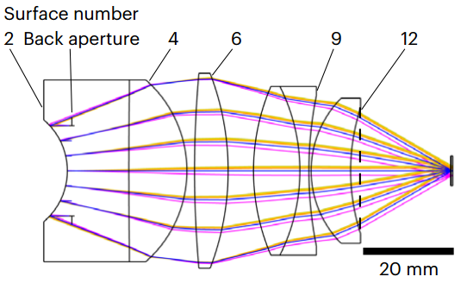
\includegraphics[width=.98\textwidth,height=.25\textheight,keepaspectratio]{Figure/ZemaxSimulation/布局图_01.png}
%                 \vspace{2pt}
%                 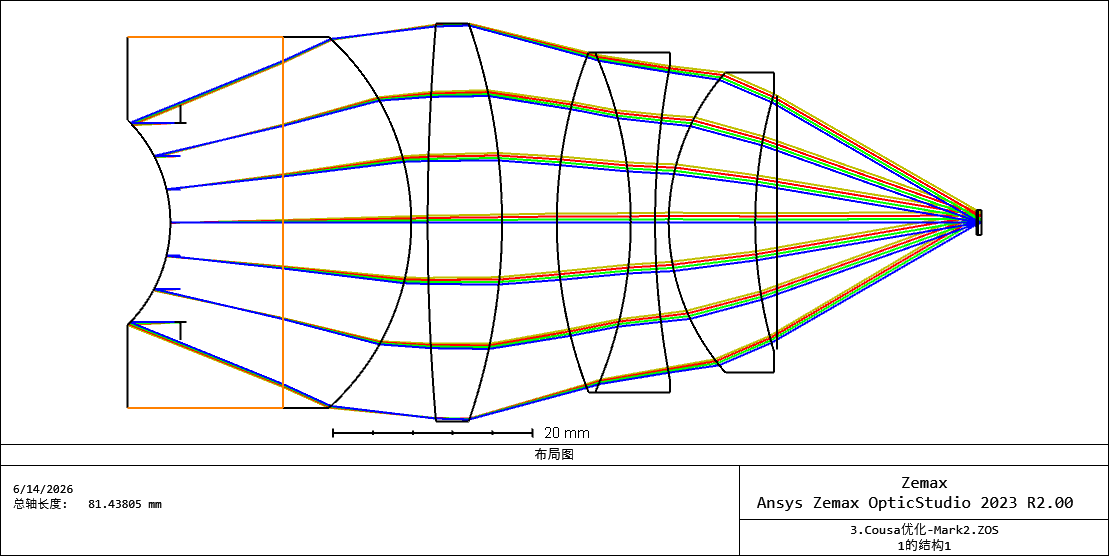
\includegraphics[width=.98\textwidth,height=.24\textheight,keepaspectratio]{Figure/ZemaxSimulation/布局图_02.png}
%                 \caption{上:文献参数(01)；下:我的 Zemax 优化参数(02)}
%                 \label{fig:cousa_layout_compare}
%             \end{figure}
%         \end{column}
%         \hfill
%         \begin{column}{.49\textwidth}
%             \begin{block}{本章对比对象}
%                 \begin{itemize}
%                     \item \textbf{01}:按文献公开参数重建的 Zemax 结果。
%                     \item \textbf{02}:在同一目标下进一步优化后的参数结果。
%                 \end{itemize}
%             \end{block}

%             \begin{block}{关注的四类指标}
%                 \begin{itemize}
%                     \item 布局图:看长工作距下的结构分配。
%                     \item RMS / OTF:看像质随视场的变化。
%                     \item 网格畸变:看 3$^\circ$ 与 5$^\circ$ 视场的几何失真。
%                     \item 斯特列尔比:看是否维持在衍射极限附近。
%                 \end{itemize}
%             \end{block}

%             \textbf{主线问题:}在保持 Cousa 长工作距设计目标的同时，优化后的参数是否让全视场像质更均匀、可用范围更大。
%         \end{column}
%     \end{columns}
% \end{frame}

\englishtitle{Layout}
\begin{frame}{布局图对比}
    \label{3.1}
    \framerefbox{Yu, C.-H. et al. Nature Methods 21, 132--141 (2024). DOI: 10.1038/s41592-023-02098-1}
    \begin{columns}[T]
        \begin{column}{.49\textwidth}
            \begin{figure}
                \centering
                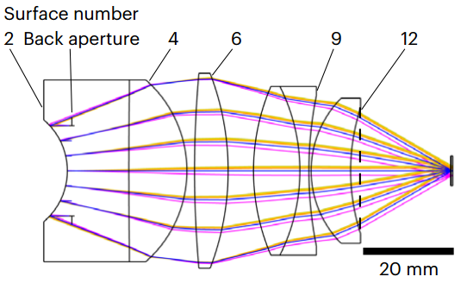
\includegraphics[width=\textwidth,height=.40\textheight,keepaspectratio]{Figure/ZemaxSimulation/布局图_01.png}
                \caption{Cousa物镜设计图}
                \label{fig:cousa_layout_lit}
            \end{figure}
        \end{column}
        \hfill
        \begin{column}{.49\textwidth}
            \begin{figure}
                \centering
                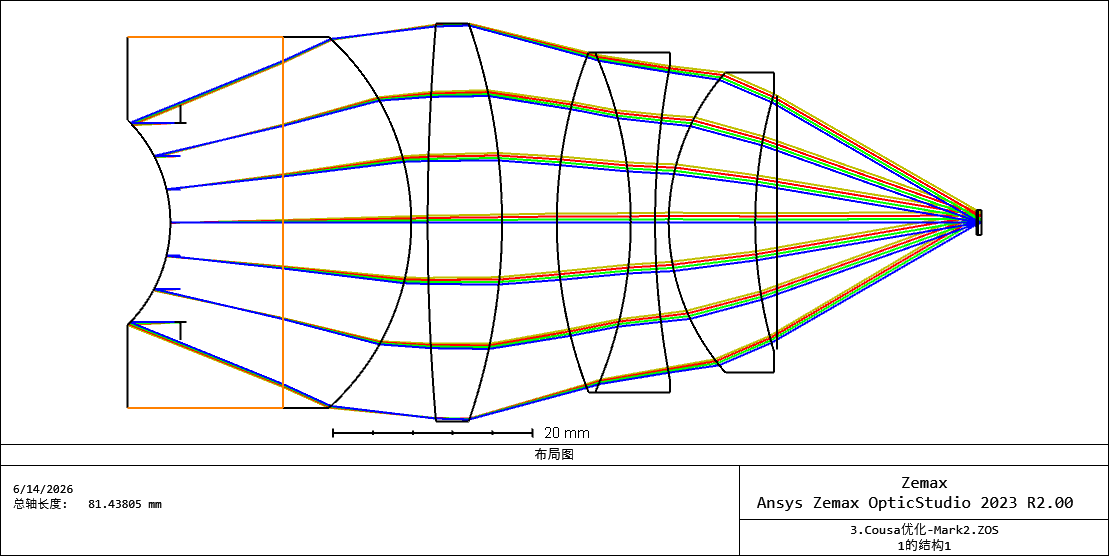
\includegraphics[width=\textwidth,height=.40\textheight,keepaspectratio]{Figure/ZemaxSimulation/布局图_02.png}
                \caption{优化后设计图}
                \label{fig:cousa_layout_opt}
            \end{figure}
        \end{column}
    \end{columns}

    \vspace{-3pt}
    \begin{itemize}
        \item 使用Zemax重新设计Cousa物镜
    \end{itemize}
\end{frame}

\englishtitle{Wavefront Error Comparison}
\begin{frame}{RMS 波前误差:文献参数与优化参数对比}
    \label{3.2}
    \begin{figure}
        \centering
        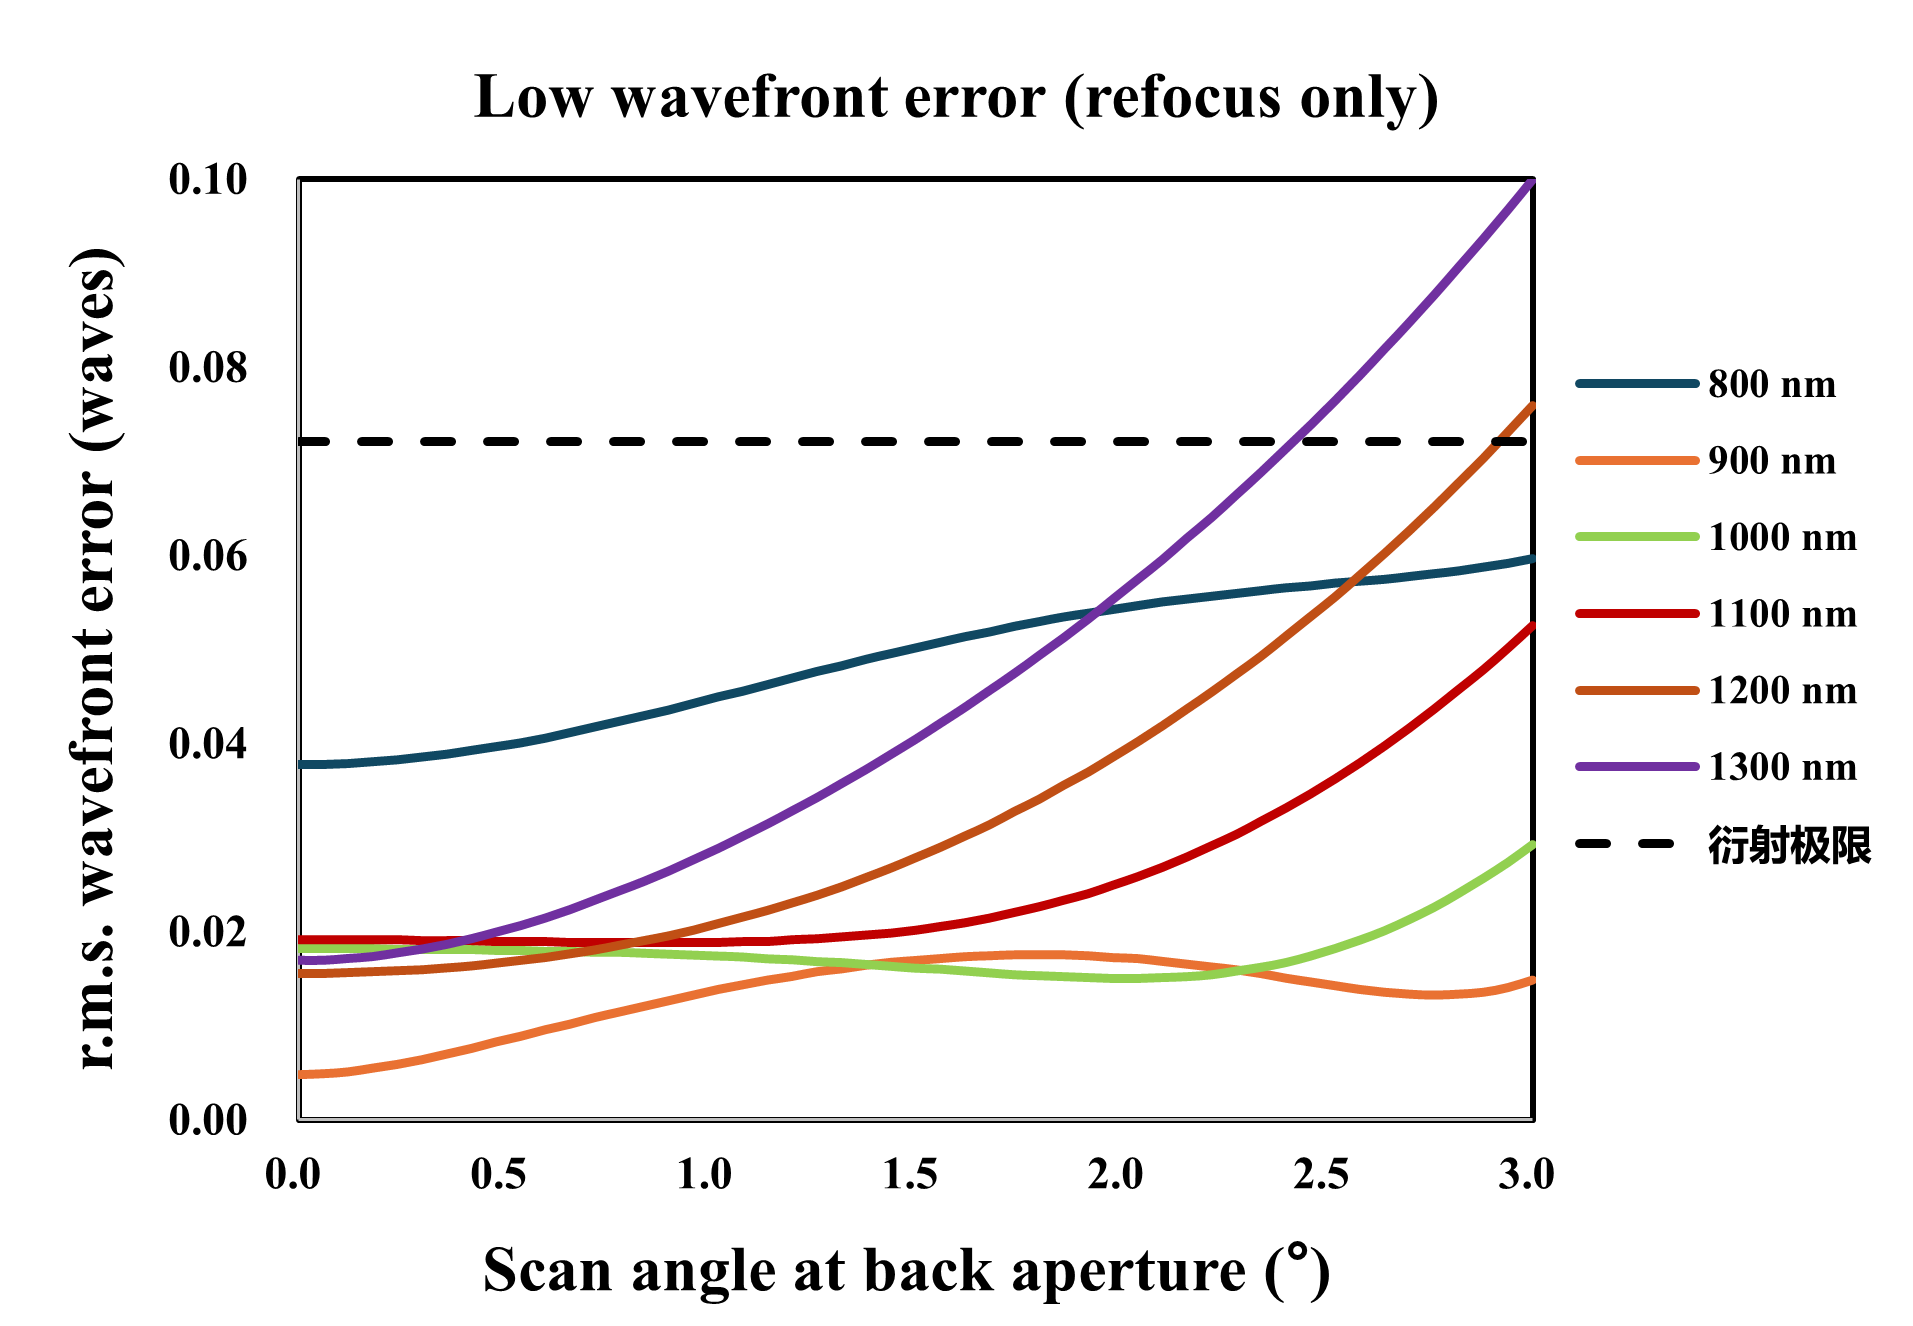
\includegraphics[width=.50\textwidth,height=.31\textheight,keepaspectratio]{Figure/ZemaxSimulation/RMS_01.png}\hfill
        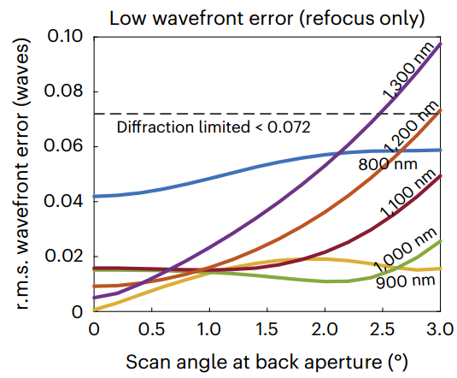
\includegraphics[width=.50\textwidth,height=.31\textheight,keepaspectratio]{Figure/ZemaxSimulation/RMS_02.png}
        \caption{左:文献参数重建的 RMS wavefront error；右:优化后参数的 RMS wavefront error}
        \label{fig:cousa_rms_compare}
    \end{figure}

    \vspace{-2pt}
    \begin{columns}[T]
        \begin{column}{.52\textwidth}
            \begin{itemize}
                \item 文献图中给出的判据是 RMS wavefront error 低于约 0.072 waves 时可视作接近衍射极限。
                \item 重建结果可以作为基准，判断 Cousa 原始公开设计在主工作视场中的误差抬升趋势。
            \end{itemize}
        \end{column}
        \begin{column}{.48\textwidth}
            \begin{itemize}
                \item 我的优化结果把主要工作波段压到更低的 RMS 水平，并让随视场增长的趋势更平缓。
                \item 这说明优化并不只是改善轴上点，而是提升了扫描过程中的全场一致性。
            \end{itemize}
        \end{column}
    \end{columns}
\end{frame}

\englishtitle{RMS and OTF Across Field}
\begin{frame}{RMS 与 OTF 随视场变化:优化后的全场表现}
    \label{3.3}
    \begin{columns}[T]
        \begin{column}{.36\textwidth}
            \begin{figure}
                \centering
                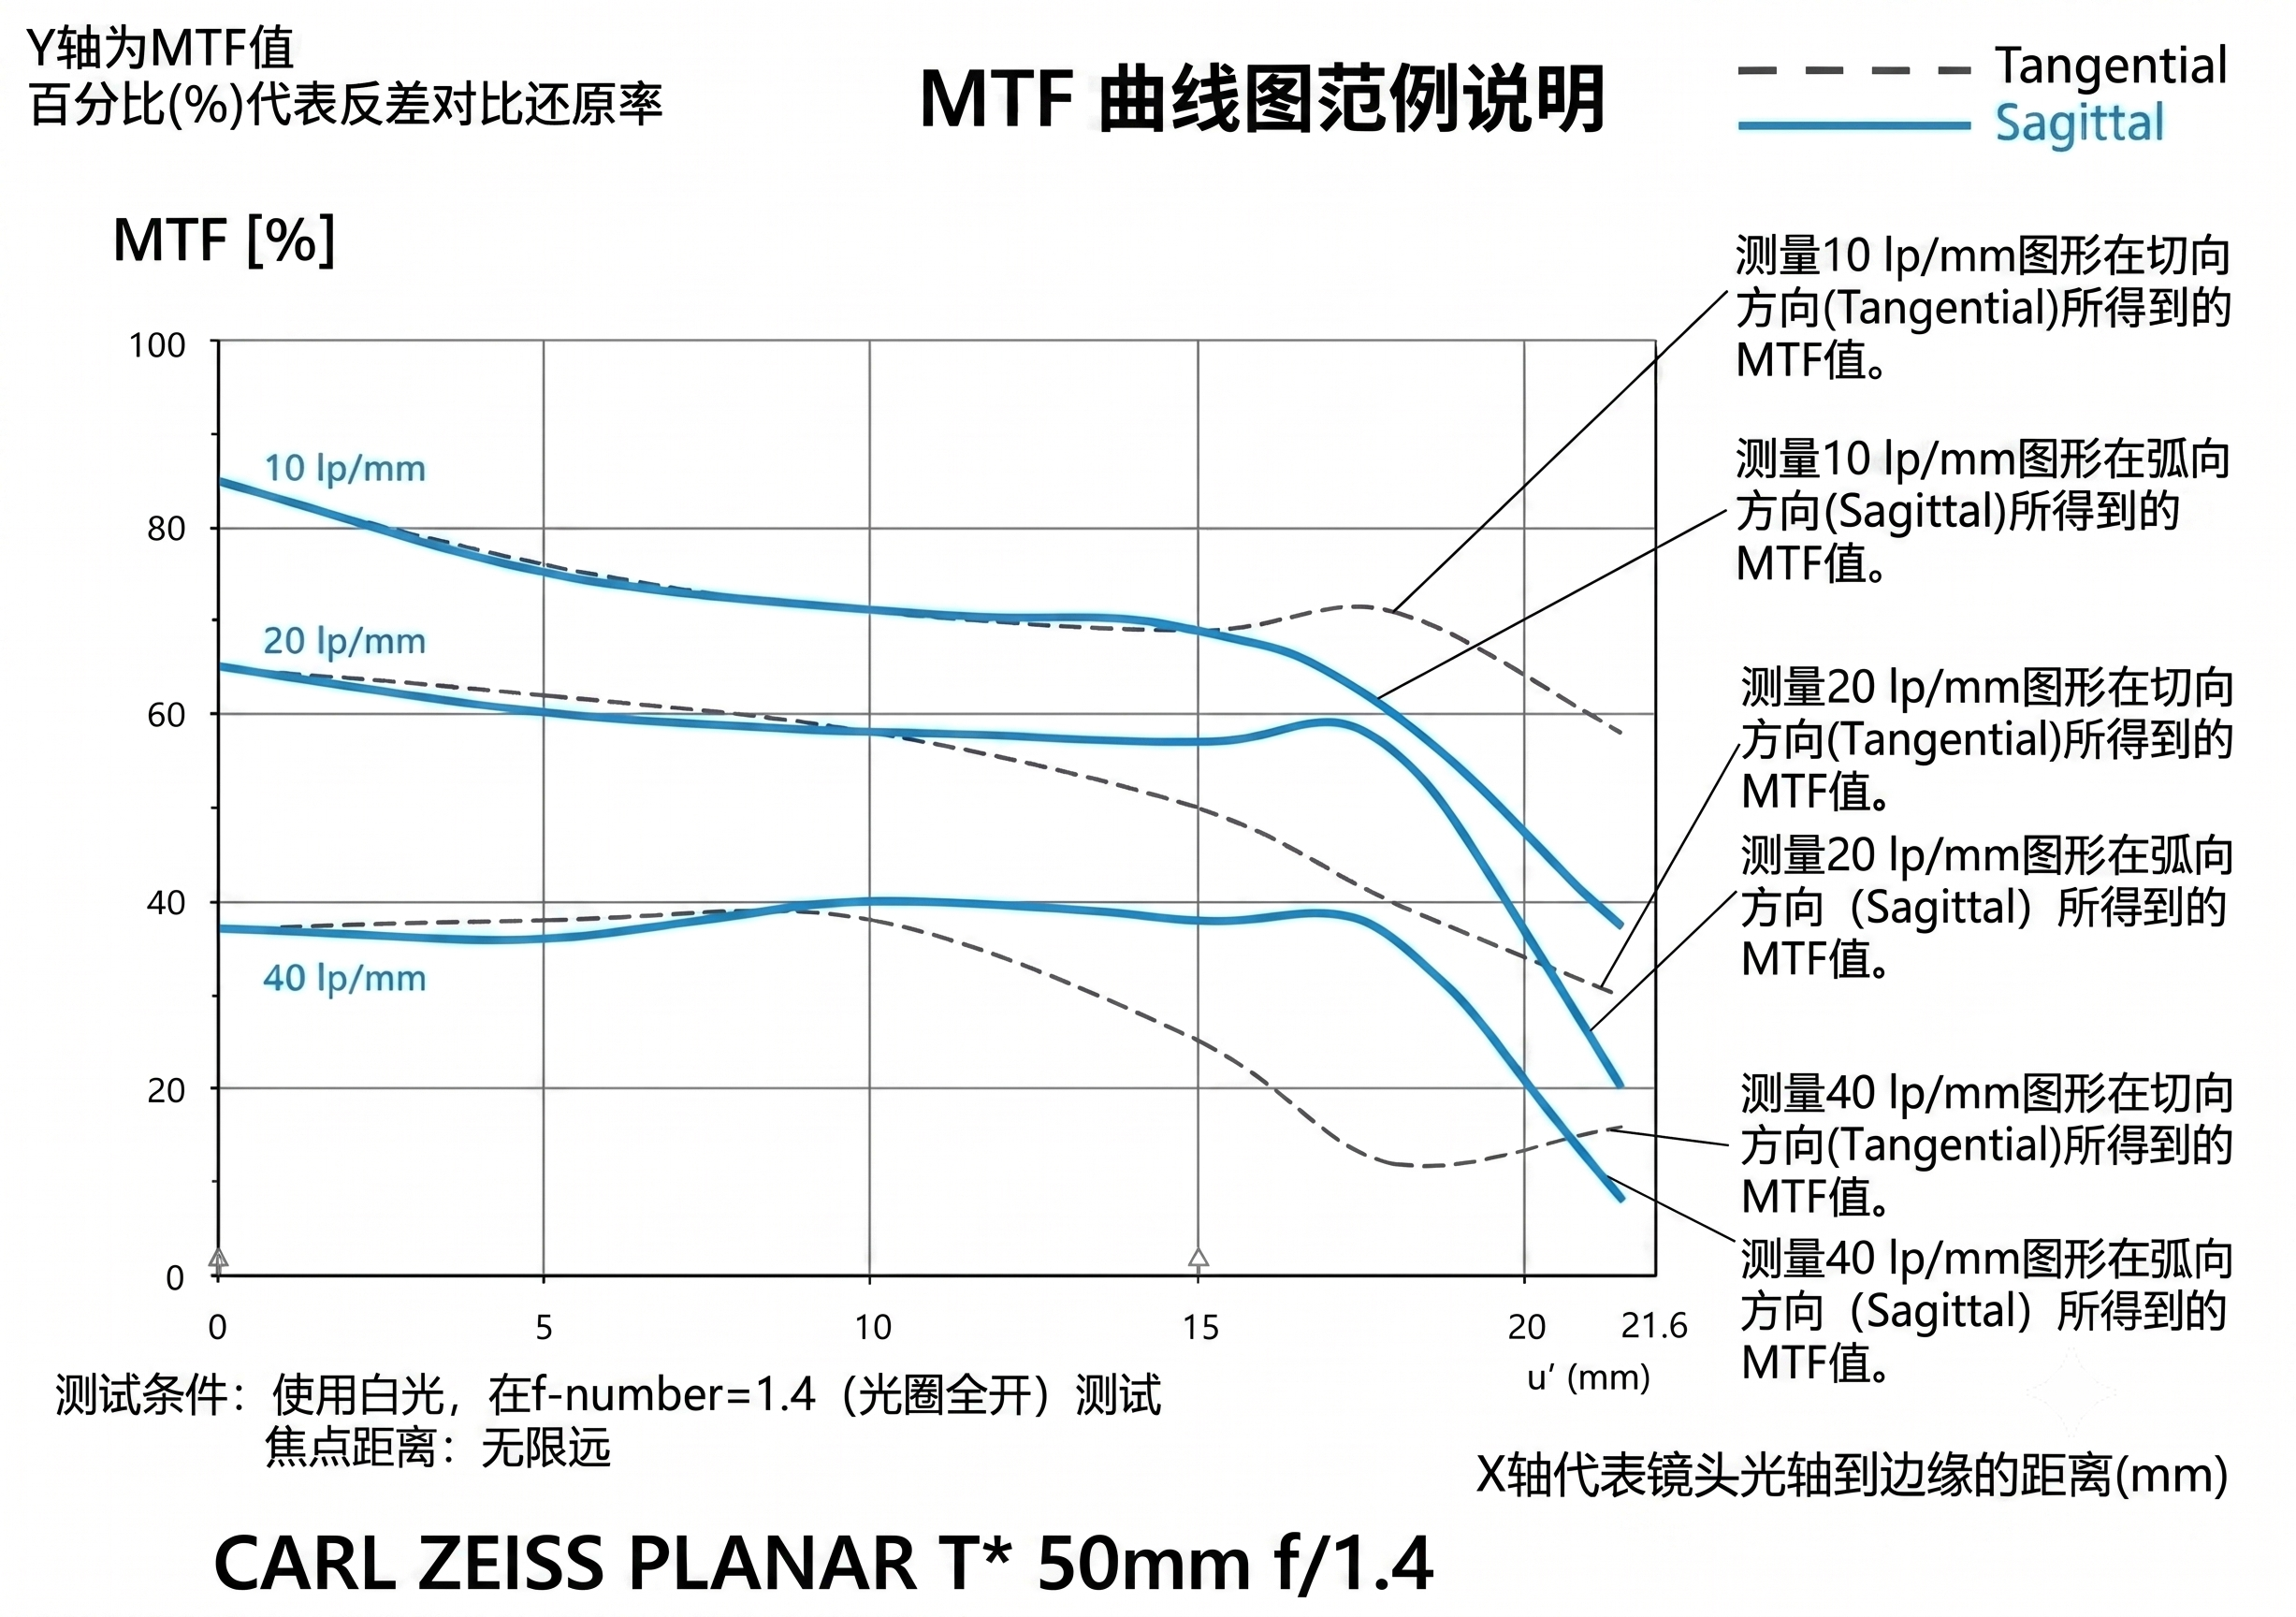
\includegraphics[width=\textwidth,height=.58\textheight,keepaspectratio]{Figure/ZemaxSimulation/MTF.png}
                \caption{MTF 曲线读法示意:切向/弧矢方向对比度传递}
                \label{fig:cousa_mtf_explain}
            \end{figure}
        \end{column}
        \hfill
        \begin{column}{.64\textwidth}
            \begin{figure}
                \centering
                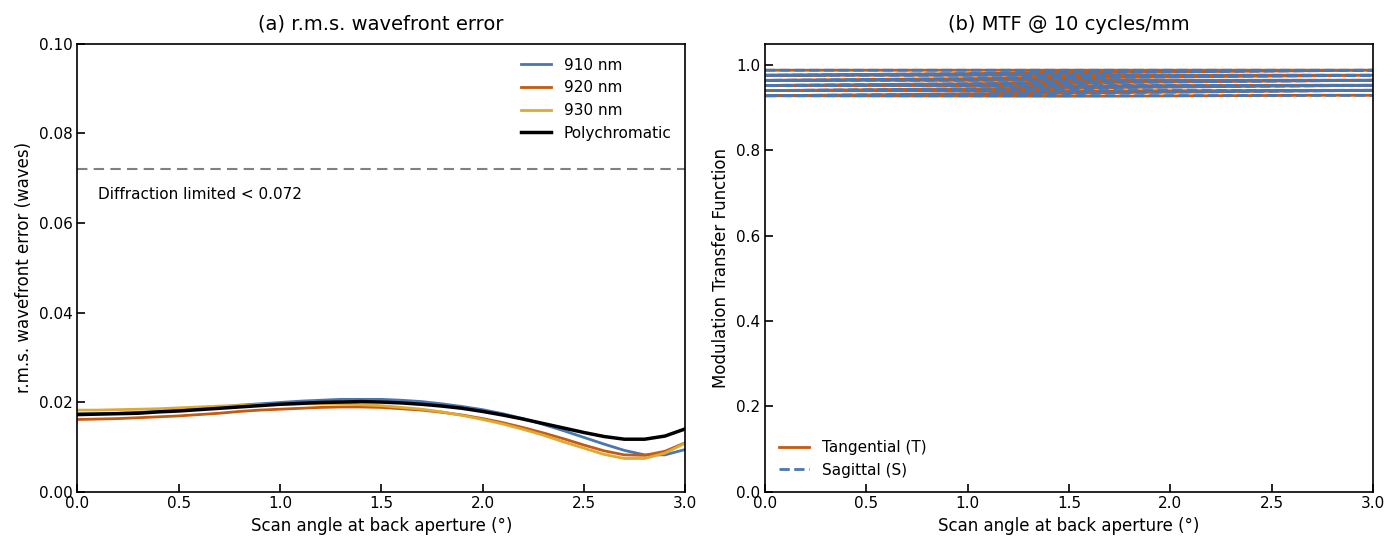
\includegraphics[width=\textwidth,height=.58\textheight,keepaspectratio]{Figure/ZemaxSimulation/RMS_03.png}
                \caption{优化后 RMS 与 10 cycles/mm OTF 随扫描视场变化}
                \label{fig:cousa_rms_otf_opt}
            \end{figure}
        \end{column}
    \end{columns}

    \vspace{-4pt}
    \begin{itemize}
        \item 左图用于说明 OTF/MTF 读图方式；右图则把优化后的波前误差和 10 cycles/mm 对比度保持能力放在同一页里。
        \item 从结果看，优化后 910/920/930 nm 三条曲线在主视场内都维持较低 RMS，切向与弧矢 OTF 也接近 1。
        \item 这意味着优化后的 Cousa 仿真不仅接近衍射极限，而且在扫描到边场时仍保持很高的低频结构还原能力。
    \end{itemize}
\end{frame}

\englishtitle{Distortion Comparison}
\begin{frame}{网格畸变:标准 3$^\circ$ 与扩展 5$^\circ$ 视场}
    \label{3.4}
    \begin{columns}[T]
        \begin{column}{.50\textwidth}
            \begin{figure}
                \centering
                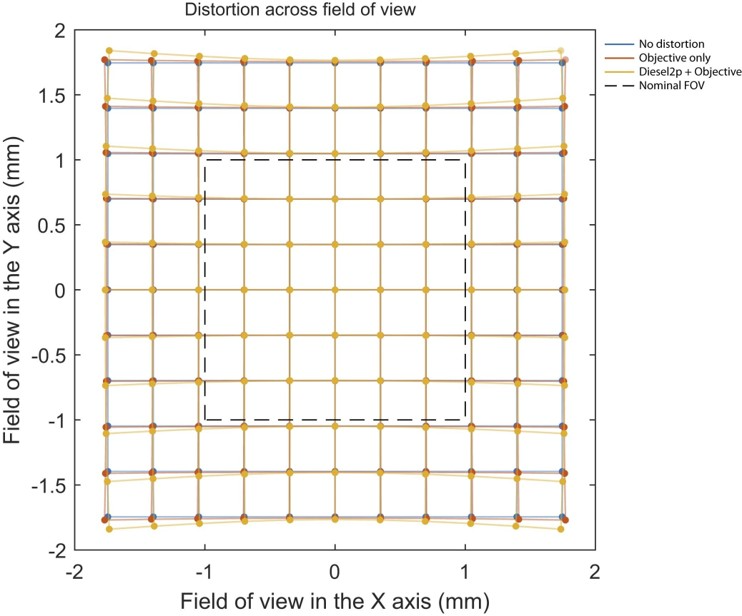
\includegraphics[width=\textwidth,height=.44\textheight,keepaspectratio]{Figure/ZemaxSimulation/网格畸变_01.png}
                \caption{Cousa物镜扫描视场内畸变，虚线框内为标准 $\pm 3^\circ$ 视场，整体为$\pm 5^\circ$ 视场}
                \label{fig:cousa_distortion_lit}
            \end{figure}
        \end{column}
        \hfill
        \begin{column}{.50\textwidth}
            \begin{figure}
                \centering
                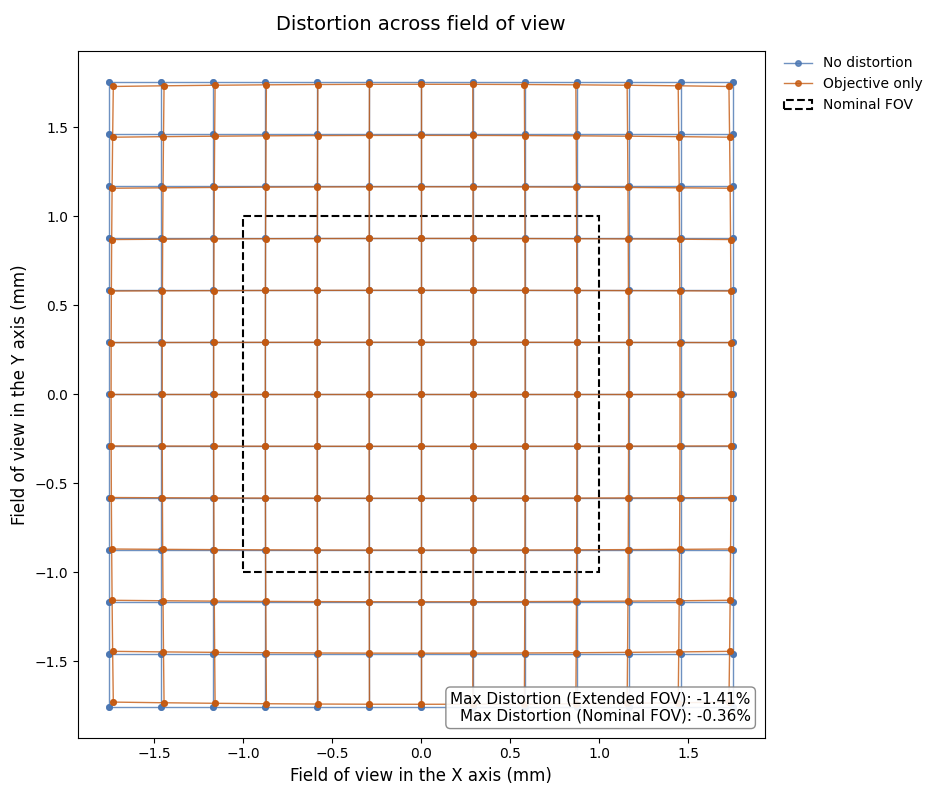
\includegraphics[width=\textwidth,height=.44\textheight,keepaspectratio]{Figure/ZemaxSimulation/网格畸变_02.png}
                \caption{优化后$\pm 5^\circ$ 扩展视场，在$\pm 3^\circ$ 视场下仍保持较低畸变}
                \label{fig:cousa_distortion_opt}
            \end{figure}
        \end{column}
    \end{columns}

    \vspace{-4pt}
    \begin{itemize}
        \item 虚线框表示标准 $\pm 3^\circ$ 扫描工作区，框外则对应更大的扩展视场评估。
        \item 标准视场最大畸变约为 0.36\%，扩展 $\pm 5^\circ$ 视场最大畸变约为 1.41\%。
    \end{itemize}
\end{frame}

\englishtitle{Strehl Ratio Comparison}
\begin{frame}{斯特列尔比:是否稳定维持在衍射极限附近}
    \label{3.5}
    \begin{columns}[T]
        \begin{column}{.34\textwidth}
            \begin{figure}
                \centering
                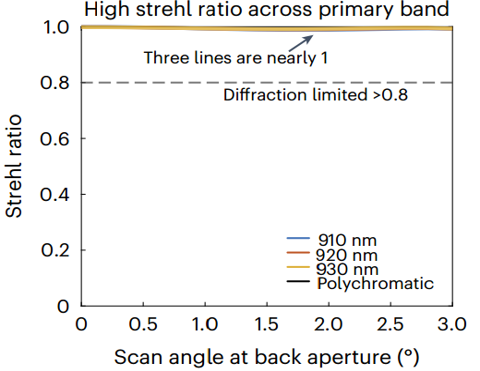
\includegraphics[width=\textwidth,height=.46\textheight,keepaspectratio]{Figure/ZemaxSimulation/斯特列尔比_01.png}
                \caption{文献参数重建结果}
                \label{fig:cousa_strehl_lit}
            \end{figure}
        \end{column}
        \hfill
        \begin{column}{.66\textwidth}
            \begin{figure}
                \centering
                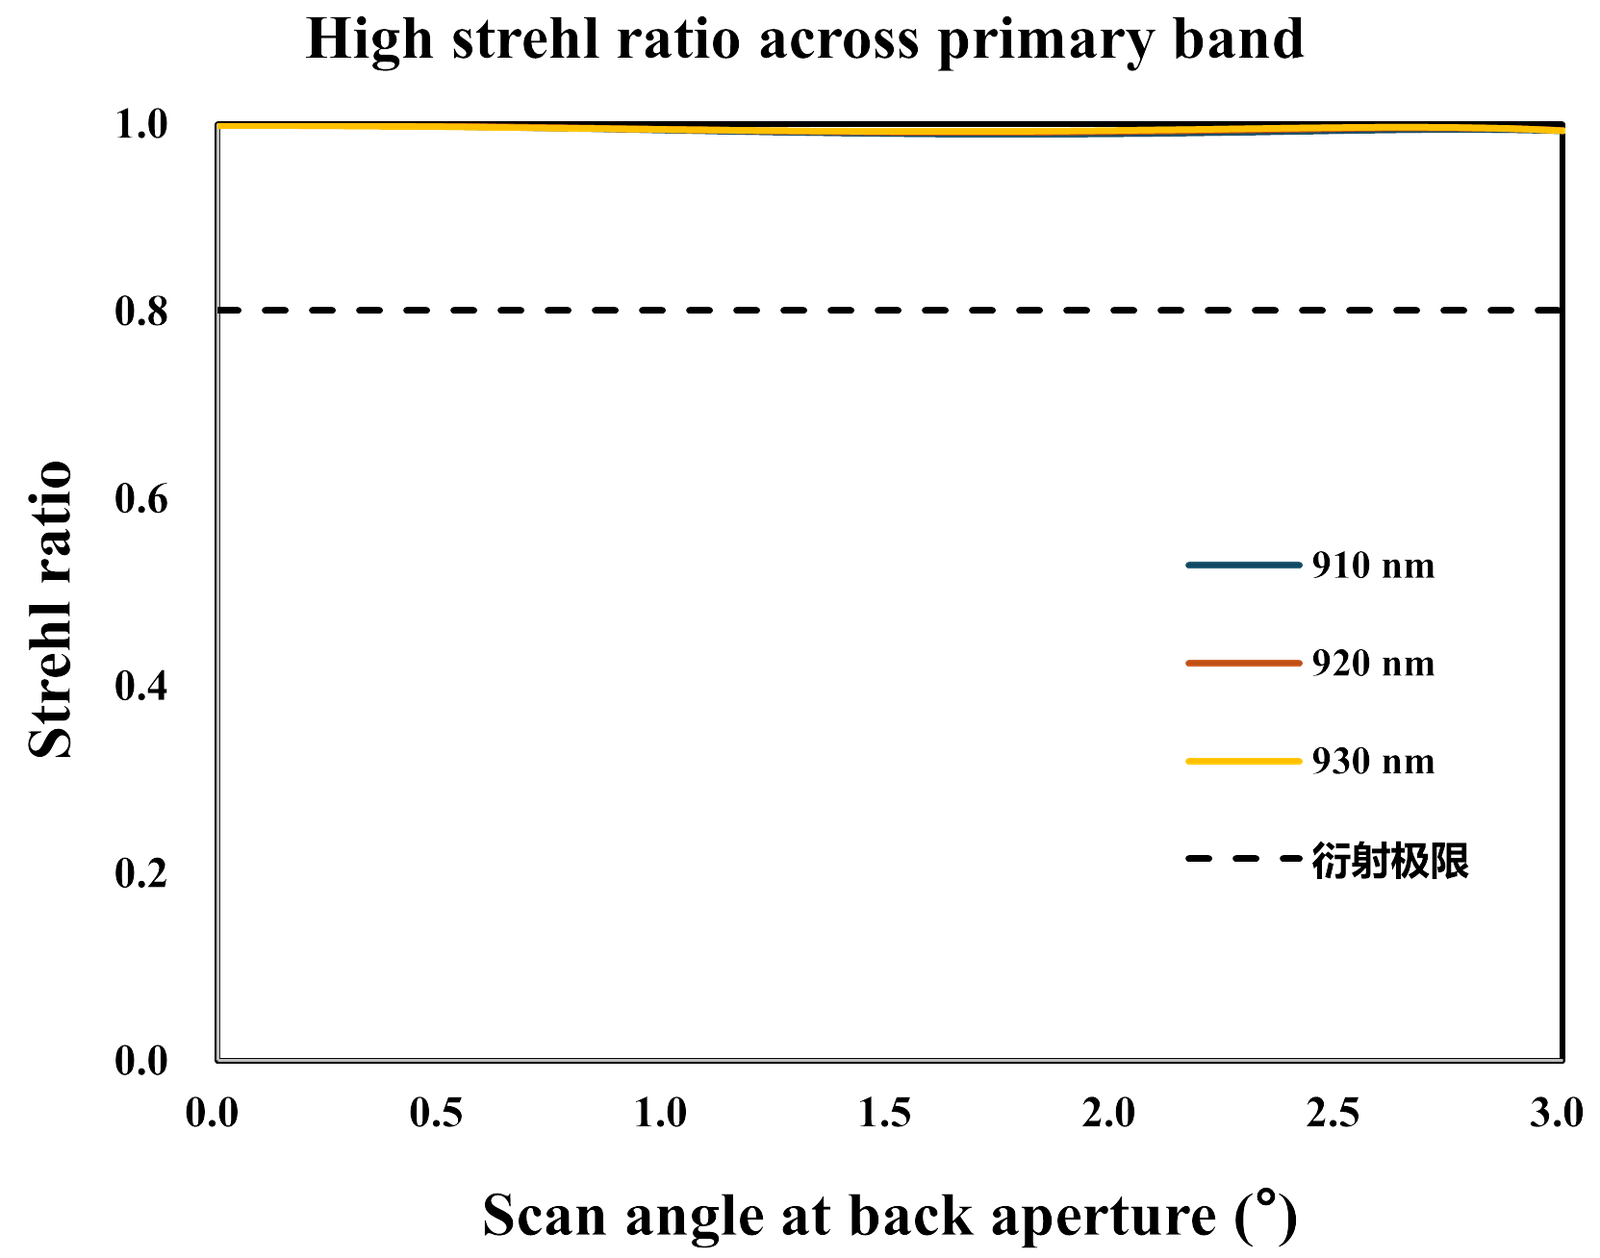
\includegraphics[width=\textwidth,height=.52\textheight,keepaspectratio]{Figure/ZemaxSimulation/斯特列尔比_02.png}
                \caption{优化后结果:主工作波段的 Strehl 几乎贴近 1}
                \label{fig:cousa_strehl_opt}
            \end{figure}
        \end{column}
    \end{columns}

    \vspace{-5pt}
    \begin{itemize}
        \item Strehl ratio 高于 0.8 通常可视作达到衍射极限附近；而优化后的三条工作波长曲线几乎都贴近 1。
        \item 这和前面的低 RMS、接近 1 的 OTF 是一致的，说明优化后的 Cousa 设计在主视场内具备很强的波前保真度。
        \item 对长工作距多光子物镜来说，这一点尤其重要，因为它意味着放宽机械空间后并没有明显牺牲主视场的像质上限。
    \end{itemize}
\end{frame}


% -----------------------------------------------------------------------------

\nonumberframe
\begin{frame}{Thank you}
\label{thanks}
\begin{center}
\begin{minipage}{1\textwidth}
    \setbeamercolor{mybox}{fg=white, bg=black!50!blue}
 \begin{beamercolorbox}[wd=0.70\textwidth, rounded=true, shadow=true]{mybox}
\LARGE \centering Thank you for listening!
\end{beamercolorbox}
 \end{minipage}
\end{center}
\end{frame}

% -----------------------------------------------------------------------------
\end{document}  %文档结束
